% #############################################################################
% This is the MAIN DOCUMENT of the Thesis MSc TEMPLATE.
% The content for the Thesis MSc is to be written in separate documents
% located in the folder ./Chapters
%         Aknowledgments.tex
%         Abstract.tex
%         KeyWords.tex
%         Resumo.tex
%         PalavrasChave.tex
%         Acronyms.tex
%         Front_Cover.tex
%         Chapter_1.tex ....Chapter_2 .....
%         ApendixA.tex ... ApendixB.tex...
% -----------------------------------------------------------------------------
% The class "istulthesis" is based on the standard LaTeX 'report' class.
% It can be used for Instituto Superior Tecnico thesis, as it follows the 
% regulations published by the Scientific Council of IST.
% The class defines the document style. 
% IST requires the thesis to be written in Arial or similar. 
% Two arguments in '\documentclass' allow you to define the thesis font: 
% 'Helvetica' and 'AvantGarde', which transforms 
% the default LaTeX font into Helvetica or AvantGarde, respectively.
% #############################################################################
% The document is automatically set for english or portuguese by just selecting
% the MAIN LANGUAGE in file 'Thesis-MSc-Preamble_commands.tex' 
% #############################################################################
% Thesis-MSc
% Version 3.1, February 2021
% BY: Prof. Rui Santos Cruz, rui.s.cruz@tecnico.ulisboa.pt
% #############################################################################
% !TEX root = ./main.tex
% -----------------------------------------------------------------------------
%
%\documentclass[defaultstyle,10pt,Helvetica,oneside]{istulthesis}
\documentclass[defaultstyle,10pt,Helvetica,twoside,openright]{istulthesis}
%
% -----------------------------------------------------------------------------
% The Preamble document contains all the necessary Packages for typesetting
% Modify it to suit your needs
% -----------------------------------------------------------------------------
% #############################################################################
% Preamble for Thesis-MSc in English or Portuguese
% Required Packages and commands
% --> Please Choose the MAIN LANGUAGE for the Thesis in package BABEL (below)
% !TEX root = ./main.tex
% #############################################################################
% Thesis-MSc
% Version 3.1, February 2021
% BY: Prof. Rui Santos Cruz, rui.s.cruz@tecnico.ulisboa.pt
% #############################################################################
%
% -----------------------------------------------------------------------------
% PACKAGES ucs, utf8x, babel, iflang:
% -----------------------------------------------------------------------------
% The 'ucs' package provides support for using UTF-8 in LaTeX documents. 
% However in most situations it is not required.
\usepackage{ucs}
% The 'utf8x' package contains support for using UTF-8 as input encoding. 
\usepackage[utf8x]{inputenc}
% The 'babel' package may correct some hyphenation issues of LaTeX. 
% Select your MAIN LANGUAGE for the Thesis with the 'main=' option.
\usepackage[main=english,portuguese]{babel}
% The 'iflang' package is used to help determine the language being used. 
\usepackage{iflang}

% -----------------------------------------------------------------------------
% PACKAGE scrbase:
% -----------------------------------------------------------------------------
% The 'scrbase' package is used to help redefining document structure.
\usepackage{scrbase}
% -----------------------------------------------------------------------------
% PACKAGE mathtools, amsmath, amsthm, amssymb, amsfonts, nicefrac:
% -----------------------------------------------------------------------------
% These packages are typically required. 
% Among many other things they add the possibility to put symbols in bold
% by using \boldsymbol (not \mathbf); defines additional fonts and symbols;
% adds the \eqref command for citing equations.
\usepackage{mathtools, amsmath, amsthm, amssymb, amsfonts}
\usepackage{nicefrac}
%
% -----------------------------------------------------------------------------
% PACKAGE tikz:
% -----------------------------------------------------------------------------
% Tikz  for creating graphics programmatically.
\usepackage{tikz}
\usetikzlibrary{shapes.geometric, arrows, positioning}
% -----------------------------------------------------------------------------
% PACKAGES array, booktabs, multirow, colortbl, spreadtab:
% -----------------------------------------------------------------------------
% These packages are most usefull for advanced tables. 
% 'multirow' allows to join rows throuhg the command \multirow which works
% similarly with the command \multicolumn.
% The 'colortbl' package allows to color the table (foreground and background)
% The package 'booktabs' provide some additional commands to enhance
% the quality of tables
% The 'longtable' package is only required when tables extend beyond the length
% of one page, which typically does not happen and should be avoided
\usepackage{array}
\usepackage{booktabs}
\usepackage{multirow}
\usepackage{colortbl}
\usepackage{spreadtab}
\usepackage{longtable}
\usepackage{pdflscape}
\usepackage{float}
% -----------------------------------------------------------------------------
% PACKAGES graphicx, subfigure:
% -----------------------------------------------------------------------------
% The package 'graphicx' supports formats PNG and JPG.
% Package 'subfigure' allows to place figures within figures with own caption. 
% For each of the subfigures use the command \subfigure.
\usepackage{graphicx}
\usepackage[hang,small,bf,tight]{subfigure}
\usepackage{amsmath}
\usepackage{caption}
%\usepackage{subcaption}
\usepackage{multirow}
\usepackage{physics}
\usepackage[a4paper, total={6in, 8in}]{geometry}
 \usepackage{tablefootnote}



\DeclareMathOperator*{\argmin}{argmin}   % Jan Hlavacek
\DeclareMathOperator*{\argmax}{argmax}   % Jan Hlavacek

% -----------------------------------------------------------------------------
% PACKAGE caption:
% -----------------------------------------------------------------------------
% The 'caption' package offers customization of captions in floating 
% environments such figure and table
% \usepackage[hang,small,bf]{caption}
\usepackage[format=hang,labelfont=bf,font=small]{caption} 
% the following customization adds vertical space between caption and the table
\captionsetup[table]{skip=10pt}
%
% -----------------------------------------------------------------------------
% PACKAGE algorithmic, algorithm, algorithm2e:
% -----------------------------------------------------------------------------
% These packages are required if you need to describe an algorithm.
% The preference is for using 'algorithm2e'
%\usepackage{algorithmic}
%\usepackage[chapter]{algorithm}
\usepackage[ruled,vlined,algochapter,norelsize,\languagename]{algorithm2e}
%
% -----------------------------------------------------------------------------
% PACKAGE listings
% -----------------------------------------------------------------------------
% These packages are required if you need to list code snippets.
\usepackage{listings}
% Nicely syntax highlighted m-code in LaTeX documents with stylefile mcode.sty
% http://www.mathworks.com/matlabcentral/fileexchange/8015-m-code-latex-package
\usepackage[numbered]{mcode}
%
% -----------------------------------------------------------------------------
% Re-define listings captions and titles based on language.
\newcaptionname{portuguese}{\lstlistingname}{Listagem} % Listings CAPTIONS
\newcaptionname{portuguese}{\lstlistlistingname}{Listagens} % LIST of LISTINGS
%
% -----------------------------------------------------------------------------
% PACKAGE csquotes
% -----------------------------------------------------------------------------
% Quotation helper package
\usepackage{csquotes}
%
% -----------------------------------------------------------------------------
% PACKAGE todonotes
% -----------------------------------------------------------------------------
% Create TODO Notes in text
% The notes can be made invisible by just using the 'disable' option:
\usepackage[textwidth=2cm, textsize=small]{todonotes}
%\usepackage[textwidth=2cm, textsize=small, disable]{todonotes}
\setlength{\marginparwidth}{2cm}
%
% -----------------------------------------------------------------------------
% PACKAGE changes
% -----------------------------------------------------------------------------
% Track changes in document (changes in pdf preview).
%% Use "final" option to make all tracking markups invisible.
%\usepackage[authormarkup=superscript,authormarkuptext=id,markup=underlined,ulem={ULforem,normalbf},final]{changes}
\usepackage[authormarkup=superscript,authormarkuptext=id,markup=underlined,ulem={ULforem,normalbf}]{changes}
% commands:
% \added[id=xx]{text}
% \deleted[id=xx]{text}
% \replaced[id=xx]{deleted text}{added text}
% -----------------------------------------------------------------------------
% PACKAGES xcolor, color
% -----------------------------------------------------------------------------
% These packages are required for list code snippets.
\usepackage{xcolor}
\usepackage{color}
% The following special color definitions are used in the IST Thesis
\definecolor{forestgreen}{RGB}{34,139,34}
\definecolor{orangered}{RGB}{239,134,64}
\definecolor{lightred}{rgb}{1,0.4,0.5}
\definecolor{orange}{rgb}{1,0.45,0.13}	
\definecolor{darkblue}{rgb}{0.0,0.0,0.6}
\definecolor{lightblue}{rgb}{0.1,0.57,0.7}
\definecolor{gray}{rgb}{0.4,0.4,0.4}
\definecolor{lightgray}{rgb}{0.95, 0.95, 0.95}
\definecolor{darkgray}{rgb}{0.4, 0.4, 0.4}
\definecolor{editorGray}{rgb}{0.95, 0.95, 0.95}
\definecolor{editorOcher}{rgb}{1, 0.5, 0} % #FF7F00 -> rgb(239, 169, 0)
\definecolor{chaptergrey}{rgb}{0.6,0.6,0.6}
\definecolor{editorGreen}{rgb}{0, 0.5, 0} % #007C00 -> rgb(0, 124, 0)
\definecolor{olive}{rgb}{0.17,0.59,0.20}
\definecolor{brown}{rgb}{0.69,0.31,0.31}
\definecolor{purple}{rgb}{0.38,0.18,0.81}
%
% -----------------------------------------------------------------------------
% PACKAGE setspace:
% ----------------------------------------------------------------------------
% Provides support for setting the spacing between lines in a document. 
% Package options include single spacing, one half spacing, and double spacing. 
% Alternatively the spacing can be changed as required with:
% \singlespacing, \onehalfspacing, and \doublespacing commands
\usepackage{setspace}
%
% -----------------------------------------------------------------------------
% PACKAGE paralist
% -----------------------------------------------------------------------------
% This package provides the 'inparaenum' environment for inline lists
\usepackage{paralist}
% usage:
% \begin{inparaenum}[(a)]
% \item bla
% \item bla, bla
% \end{inparaenum}
% -----------------------------------------------------------------------------
% PACKAGE cite:
% -----------------------------------------------------------------------------
% The 'cite' package will result in citation numbers being automatically
% sorted and properly "ranged". i.e.,
% [1], [2], [5]--[7], [9]
\usepackage{cite}
%
% -----------------------------------------------------------------------------
% PACKAGE acronym:
% -----------------------------------------------------------------------------
% The package 'acronym' garantees that all acronyms definitions are 
% given at the first usage. 
% IMPORTANT: do not use acronyms in titles/captions; otherwise the definition 
% will appear on the table of contents.
\usepackage[printonlyused]{acronym}
%
% -----------------------------------------------------------------------------
% PACKAGE hyperref
% -----------------------------------------------------------------------------
% Set links for references and citations in document
\usepackage{hyperref}
% pre-configuration of hyperref
\hypersetup{ colorlinks=true,
             citecolor=cyan,
             linkcolor=darkgray,
             urlcolor=teal,
             breaklinks=true,
             bookmarksnumbered=true,
             bookmarksopen=true,
}
%
% -----------------------------------------------------------------------------
% PACKAGE url:
% -----------------------------------------------------------------------------
% Provides better support for handling and breaking URLs.
\usepackage{url} 
%
% -----------------------------------------------------------------------------
% PACKAGE Cleveref:
% -----------------------------------------------------------------------------
% Clever Referencing of document parts
% use \Cref[], or \cref[] for referencing items (Figures, Tables, Algorythms, 
% Equations, Chapters, Sections, etc. No need to write the Name of the item. 
% Note: portuguese is supported through "brazilian" option
\usepackage[\IfLanguageName{english}{english}{brazilian}]{cleveref}
%
% -----------------------------------------------------------------------------
% PACKAGE enumitem:
% -----------------------------------------------------------------------------
%For enhanced enumeration of lists
%\usepackage{enumitem}
\usepackage[shortlabels]{enumitem}
\setlist[description]{leftmargin=\parindent,labelindent=\parindent,itemsep=1pt,parsep=0pt,topsep=0pt}
%
% #############################################################################
% GLOBAL FORMATTING OF THE THESIS DOCUMENT before using FANCY stuff
% Load Titlepage definition
\usepackage{./Thesis-MSc-cover-titlepage}

% Set paragraph counter to alphanumeric mode
% DO NOT CHANGE these lines, otherwise the document will not respect the Guide
\renewcommand{\theparagraph}{\Alph{paragraph}~--}
\hoffset 0in
\voffset 0in
\oddsidemargin 0 cm
\evensidemargin 0 cm
\marginparsep 0in
\topmargin -0.25cm
\textwidth 16 cm
\textheight 22.4 cm
\makeatletter
% package indentfirst says \let\@afterindentfalse\@afterindenttrue
% and we revert this modification, reinstating the original definitio
% of \@afterindentfalse
\def\@afterindentfalse{\let\if@afterindent\iffalse}
\makeatother
% -----------------------------------------------------------------------------
% PACKAGE fancyhdr:
% -----------------------------------------------------------------------------
% The fancyhdr macro package allows to customize page headers and footers.
\usepackage{fancyhdr}
\pagestyle{fancy}
\renewcommand{\chaptermark}[1]{\markboth{\thechapter.\ #1}{}}
\renewcommand{\sectionmark}[1]{\markright{\thesection\ #1}}
\fancyhf{}
%#########################################################
% Choose the positioning of the Page Number
% Only on the Center side [C]
\fancyfoot[C]{\bfseries\thepage}
% Only on the Right side [R]
%\fancyfoot[R]{\bfseries\thepage}
% In case of Double sided printing 
%\fancyfoot[LE,RO]{\bfseries\thepage}
%#########################################################
\renewcommand{\headrulewidth}{0.0pt}
\renewcommand{\footrulewidth}{0.0pt}
\addtolength{\headheight}{2pt} % make space for the rule

\fancypagestyle{plain}{%
   \renewcommand{\headrulewidth}{0pt} % and the line
   \renewcommand{\footrulewidth}{0pt}
}
\fancypagestyle{blank}{%
   \renewcommand{\headrulewidth}{0pt} % and the line
   \renewcommand{\footrulewidth}{0pt}
}
\fancypagestyle{abstract}{%
   \renewcommand{\headrulewidth}{0pt}
   \renewcommand{\footrulewidth}{0.0pt}
}
\fancypagestyle{document}{%
	\renewcommand{\headrulewidth}{0.5pt}
	\renewcommand{\footrulewidth}{0.5pt}
	\addtolength{\headheight}{2pt} % make space for the rule
}
\setcounter{secnumdepth} {5}
\setcounter{tocdepth} {5}
\renewcommand{\thesubsubsection}{\thesubsection.\Alph{subsubsection}}
\renewcommand{\subfigtopskip}{0.3 cm}
\renewcommand{\subfigbottomskip}{0.2 cm}
\renewcommand{\subfigcapskip}{0.3 cm}
\renewcommand{\subfigcapmargin}{0.2 cm}
%
% -----------------------------------------------------------------------------
% PACKAGE minitoc:
% -----------------------------------------------------------------------------
% Package 'minitoc' creates a mini-table of contents (a “minitoc”) at 
% the beginning of each chapter of a document.
% This packages are required for the \fancychapter configuration
\usepackage{minitoc}
\setcounter{minitocdepth}{1}
\setlength{\mtcindent}{24pt}
\renewcommand{\mtcfont}{\small\rm}
\renewcommand{\mtcSfont}{\small\bf}
\renewcommand*{\kernafterminitoc}{\kern0.\baselineskip\kern0.ex}
\mtcselectlanguage{\languagename} 
% Now prepare the MINITOC
\def\boxedverbatim{%
  \def\verbatim@processline{%
    {\setbox0=\hbox{\the\verbatim@line}%
    \hsize=\wd0 \the\verbatim@line\par}}%
  \@minipagetrue%%%DPC%%%
  \@tempswatrue%%%DPC%%%
  \setbox0=\vbox\bgroup\vspace*{0.2cm}\footnotesize\verbatim
}
\def\endboxedverbatim{%
  \endverbatim
  \unskip\setbox0=\lastbox %%%DPC%%%
  \hspace*{0.2cm}
  \vspace*{-0.2cm}
  \egroup
  \fbox{\box0}% <<<=== change here for centering,...
}
% Now prepare the CHAPTER Number
\newcommand*{\chapnumfont}{%
%   \usefont{T1}{\@defaultcnfont}{b}{n}\fontsize{100}{130}\selectfont%
  \usefont{T1}{pbk}{b}{n}
  \fontsize{150}{130}
  \selectfont
  \color{chaptergrey}
}
\makeatletter
\def\@makechapterhead#1{%
  \vspace*{50\p@}%
  {\parindent \z@ \raggedright \normalfont
    {\chapnumfont\ifnum \c@secnumdepth >\m@ne
%         \huge\bfseries \@chapapp\space \thechapter
        \raggedleft\bfseries \thechapter
        \par\nobreak
        \vskip 20\p@
    \fi}
    \interlinepenalty\@M
    {\raggedleft\Huge \bfseries #1\par\nobreak}
    \vskip 40\p@
  }}
\makeatother
% Now put it all together as a command \fancychapter
\newcommand{\fancychapter}[1]{\chapter{#1}\vfill\minitoc\pagebreak}
%
% #############################################################################
% ADDITIONAL COMMANDS AND CONFIGURATIONS
% #############################################################################
% This commmand allows to place horizontal lines with a custom width... 
% replaces the standard hline command
\newcommand{\hlinew}[1]{%
  \noalign{\ifnum0=`}\fi\hrule \@height #1 \futurelet
   \reserved@a\@xhline}
%   
% -----------------------------------------------------------------------------
% This command defines some marks... USEFUL FOR TABLES.
\def\Mark#1{\raisebox{0pt}[0pt][0pt]{\textsuperscript{\footnotesize\ensuremath{\ifcase#1\or *\or \dagger\or \ddagger\or%
    \mathsection\or \mathparagraph\or \|\or **\or \dagger\dagger%
    \or \ddagger\ddagger \else\textsuperscript{\expandafter\romannumeral#1}\fi}}}}
%


% -----------------------------------------------------------------------------
% The following configurations are used for LISTINGS of certain languages
\lstdefinestyle{XML} {
	language=XML,
	extendedchars=true, 
	breaklines=true,
	breakatwhitespace=true,
	emph={},
	emphstyle=\color{red},
	basicstyle=\small,
	xleftmargin=17pt,
	columns=fullflexible,
	commentstyle=\color{gray}\upshape,
	morestring=[b][\color{brown}]",
	morecomment=[s]{<?}{?>},
	morecomment=[s][\color{forestgreen}]{<!--}{-->},
	keywordstyle=\color{orangered},
	stringstyle=\ttfamily\color{black},
	% stringstyle=\ttfamily\color{black}\normalfont,
	tagstyle=\color{blue},
	% tagstyle=\color{darkblue}\bf,
	morekeywords={asn,action,addrType,abilityNAT,audioSampleRate,audiChannels,,bandwidth,bitmapSize,bitRate,connection,codecs,concurrentLinks,dependency,duration,frameRate,from,height,ip,id,lang,mimeType,onlineTime,peerMode,port,priority,peerProtocol,property,release,to,tier,type,transactionID,url,uploadBWlevel,version,width},
	otherkeywords={attribute,xmlns,schemaLocation,PresentationType,availabilityStartTime,availabilityEndTime,minimumUpdatePeriod,minBufferTime,UpdateTime},
}
% ----------------------------------------------------------------------------
\lstdefinelanguage{Assembler}{
	morecomment=[l];,
	keywords={ADD,ADDC,SUB,SUBB,CMP,MUL,DIV,MOD,NEG,AND,OR,NOT,XOR,TEST,BIT,SET,EI,EI0,EI1,EI2,EI3,SETC,EDMA,CLR,DI,DI0,DI1,DI2,DI3,CLRC,SHR,SHL,SHRA,SHLA,ROR,ROL,RORC,ROLC,MOV,MOVB,MOVBS,MOVP,MOVL,MOVH,SWAP,PUSH,POP,JZ,JNZ,JN,JNN,JP,JNP,JC,JNC,JV,JNV,JEQ,JNE,JLT,JLE,JGT,JGE,JA,JAE,JB,JBE,JMP,CALL,CALLF,RET,RETF,SWE,RFE,NOP},
	morekeywords={EQU,TABLE,WORD,STRING,PLACE},
} 
% ----------------------------------------------------------------------------
\lstdefinestyle{coloredASM}{
	language=Assembler,
	extendedchars=false,
	breaklines=true,
	tabsize=2,
	numberstyle=\tiny,
	numbers=left,
	breakatwhitespace=true,
	emph={},
	emphstyle=\color{red},
	fontadjust=true,
	basicstyle=\small\ttfamily,
	% basicstyle=\footnotesize\ttfamily,
	columns=fixed,
	xleftmargin=17pt,
	framexleftmargin=17pt,
	framexrightmargin=5pt,
	framexbottommargin=4pt,
	commentstyle=\color{forestgreen}\upshape,
	morestring=[b][\color{brown}]",
	keywordstyle=\color{darkblue},
	stringstyle=\ttfamily\color{black},
	literate={á}{{\'a}}1 {ã}{{\~a}}1 {â}{{\^a}}1 {é}{{\'e}}1 {É}{{\'E}}1 {ê}{{\^e}}1 {õ}{{\~o}}1 {ó}{{\'o}}1 {í}{{\'i}}1 {ç}{{\c{c}}}1 {Ç}{{\c{C}}}1,
}    
% ----------------------------------------------------------------------------
\lstdefinelanguage{CSS}{
	sensitive=true,
	morecomment=[l]{//},
	morecomment=[s]{/*}{*/},
	morestring=[b]',
	morestring=[b]",
	alsoletter={:},
	alsodigit={-},
	keywords={color,background-image:,margin,padding,font,weight,display,position,top,left,right,bottom,list,style,border,size,white,space,min,width, transition:, transform:, transition-property, transition-duration, transition-timing-function}
}
% ----------------------------------------------------------------------------
% JavaScript
\lstdefinelanguage{JavaScript}{
	morecomment=[s]{/*}{*/},
	morecomment=[l]//,
	morestring=[b]",
	morestring=[b]',
	morekeywords={typeof, new, true, false, catch, function, return, null, catch, switch, var, if, in, while, do, else, case, break}
}
% ----------------------------------------------------------------------------
\lstdefinelanguage{HTML5}{
	language=html,
	sensitive=true,	
	alsoletter={<>=-},	
	morecomment=[s]{<!-}{-->},
	tag=[s],
	otherkeywords={
	% General
	>,
	% Standard tags
	<!DOCTYPE,
	</html, <html, <head, <title, </title, <style, </style, <link, </head, <meta, />,
	% body
	</body, <body,
	% Divs
	</div, <div, </div>, 
	% Paragraphs
	</p, <p, </p>,
	% scripts
	</script, <script,
	% More tags...
	<canvas, /canvas>, <svg, <rect, <animateTransform, </rect>, </svg>, <video, <source, <iframe, </iframe>, </video>, <image, </image>, <header, </header, <article, </article},
	ndkeywords={
	% General
	=,
	% HTML attributes
	charset=, src=, id=, width=, height=, style=, type=, rel=, href=,
	% SVG attributes
	fill=, attributeName=, begin=, dur=, from=, to=, poster=, controls=, x=, y=, repeatCount=, xlink:href=,
	% properties
	margin:, padding:, background-image:, border:, top:, left:, position:, width:, height:, margin-top:, margin-bottom:, font-size:, line-height:,
	% CSS3 properties
	transform:, -moz-transform:, -webkit-transform:,
	animation:, -webkit-animation:,
	transition:,  transition-duration:, transition-property:, transition-timing-function:,
	}
}
% ----------------------------------------------------------------------------
\lstdefinestyle{htmlcssjs} {%
	% General design
	backgroundcolor=\color{editorGray},
		fontadjust=true,
	basicstyle=\small\ttfamily,   
	frame=b,
	% line-numbers
	xleftmargin={0.75cm},
	numbers=left,
	stepnumber=1,
	firstnumber=1,
	numberfirstline=true,	
	% Code design
	identifierstyle=\color{black},
	keywordstyle=\color{blue}\bfseries,
	ndkeywordstyle=\color{editorGreen}\bfseries,
	stringstyle=\color{editorOcher}\ttfamily,
	commentstyle=\color{brown}\ttfamily,
	% Code
	language=HTML5,
	alsolanguage=JavaScript,
	alsodigit={.:;},	
	tabsize=2,
	showtabs=false,
	showspaces=false,
	showstringspaces=false,
	extendedchars=true,
	breaklines=true,
	% German umlauts
	literate=%
	{Ö}{{\"O}}1
	{Ä}{{\"A}}1
	{Ü}{{\"U}}1
	{ß}{{\ss}}1
	{ü}{{\"u}}1
	{ä}{{\"a}}1
	{ö}{{\"o}}1
}
% ----------------------------------------------------------------------------
\lstdefinestyle{py} {%
	language=python,
	literate=%
	*{0}{{{\color{lightred}0}}}1
	{1}{{{\color{lightred}1}}}1
	{2}{{{\color{lightred}2}}}1
	{3}{{{\color{lightred}3}}}1
	{4}{{{\color{lightred}4}}}1
	{5}{{{\color{lightred}5}}}1
	{6}{{{\color{lightred}6}}}1
	{7}{{{\color{lightred}7}}}1
	{8}{{{\color{lightred}8}}}1
	{9}{{{\color{lightred}9}}}1,
	basicstyle=\small\ttfamily,
	numbers=left,
	% numberstyle=\tiny,
	% stepnumber=2,
	numbersep=5pt,
	tabsize=4,
	extendedchars=true,
	breaklines=true,
	keywordstyle=\color{blue}\bfseries,
	frame=b,
	commentstyle=\color{brown}\itshape,
	stringstyle=\color{editorOcher}\ttfamily,
	showspaces=false,
	showtabs=false,
	xleftmargin=17pt,
	framexleftmargin=17pt,
	framexrightmargin=5pt,
	framexbottommargin=4pt,
	backgroundcolor=\color{lightgray},
	showstringspaces=false,
}
%
% #############################################################################
% #############################################################################
\begin{document}
%
% Add PDF bookmark 
\pdfbookmark[0]{Titlepage}{Title}
% #############################################################################
% DEFINE THE Front Cover Page of Thesis-MSc
% !TEX root = ./main.tex
% #############################################################################
% Thesis-MSc
% Version 3.1, February 2021
% BY: Prof. Rui Santos Cruz, rui.s.cruz@tecnico.ulisboa.pt
% #############################################################################
%
% REQUIRED LOGO:
% The university logo image: arguments correspond to {left}{top} position. 
% IST rules determine the position to be be 2cm from top, left page edge
\univlogo{20mm}{20mm}{./imgs/IST_A_RGB_POS}
% OPTIONAL IMAGE:
% The thesis image: arguments are the start position in the page.
% You can change the image for your thesis, replacing the image name.
% If no image is desired, just comment the command
%\thesislogo{130mm}{15mm}{./imgs/INESC-ID}
%
\univname{UNIVERSIDADE DE LISBOA \\
INSTITUTO SUPERIOR TÉCNICO}
% -----------------------------------------------------------------------------
% REQUIRED: Thesis TITLE
\title{Towards improved automatic speech recognition for children}
% OPTIONAL: Thesis SUBTITLE
%\subtitle{Thesis}
%
% -----------------------------------------------------------------------------
% REQUIRED: Author
% Author full Name
\author{Thomas Rolland}
%
% -----------------------------------------------------------------------------
% REQUIRED: The SUPERVISOR(s) - maximum of two
\supervisor{Doctor Alberto Abad Gareta}
% If no co-Supervisor comment the next line
%\othersupervisor{Prof. Name of the Co-Supervisor}
%
% -----------------------------------------------------------------------------
% The official name of the course/degree. Please chose portuguese or english
% un-comment the line corresponding to your degree.
% You can add a degree name using thie following construct:
%
%\degree{Information Systems and Computer Engineering}
\degree{Thesis approved in public session to obtain the PhD Degree in Computer Science and Engineering }
%\degree{Telecommunications and Informatics Engineering}
%\degree{Engenharia de Telecomunicações e Informática}
%
\draft{Jury final classification: Pass with Distinction and Honour}
% -----------------------------------------------------------------------------
% REQUIRED: Date of examination
% Insert the Date of the Thesis discussion (format is MONTH and YEAR)
\date{2024}
%
% -----------------------------------------------------------------------------
% The following command define the author colors for Tracking Changes in doc in case you use Tracking
% the Two letters identify each author
\definechangesauthor[color=forestgreen]{MN}
\definechangesauthor[color=blue]{JO}
\definechangesauthor[color=red]{PT}

% -----------------------------------------------------------------------------
% Select 'false' when delivering the draft version of the thesis.
% The committee members should not be printed for the draft version. 
% Select 'true' after the Examination Committee has accepted the thesis as final
%\finalthesis{true}
\finalthesis{false}
%
% -----------------------------------------------------------------------------
% The members of the Examination Committee
% Normally there is only the "vogalone"
% Comment the other if not necessary
%\chairperson{Prof. Maria Luísa Torres Ribeiro Marques da Silva Coheur}
%\vogalone{Prof. Name of First Committee Member}
%\vogalone{Dr. Mathew Magimai Doss}
%\vogalthree{Eng. Name of Third Committee Member}
%
% -----------------------------------------------------------------------------
% The second page should be white with the Copyright message.
% Print Titlepage (Cover)
\maketitle
\thispagestyle{empty} % the following page without header or footer
\cleardoublepage{}
%
% -----------------------------------------------------------------------------
% PAGE NUMBERING FOR INDEXING MATTER in ROMAN
\setcounter{page}{1} \pagenumbering{roman}
\baselineskip 18pt % line spacing: -12pt for single spacing
                   %               -18pt for 1 1/2 spacing
                   %               -24pt for double spacing
% -----------------------------------------------------------------------------

% THE ABSTRACT
\pdfbookmark[0]{Abstract}{Abstract}
\begin{abstract}
	% #############################################################################
% Abstract Text
% !TEX root = ../main.tex
% #############################################################################
% reset acronyms
\acresetall
% use \noindent in firts paragraph
%\noindent Speech is a fundamental communication skill used for social interaction, express feelings and needs, among others. Unfortunately, there is an increasing number of people who suffer from debilitating speech pathologies, including children. A childhood speech disorder that is not properly diagnosed and treated can have long-term negative effects in social, communication and educational situations. Hence the importance of speech therapy.

%In recent years, machine learning has proven to have many applications in the health field, both for diagnosis and monitoring. Particularly, there is a growing interest in the development of automatic tools to assist speech-language pathologists. Furthermore, some automatic tools allow patients to do exercises outside the session with the therapist, for example at home. In the case of children, the exercises can be provided in a gamification context, which contributes to motivate them to practice more often. Most of these tools require reliable automatic speech recognition systems, as these are commonly used to provide pronunciation quality scores. However, despite recent significant improvements in the performance of automatic speech recognition systems for healthy adults, these systems' performance dramatically drops when considering speech from children and speakers with speech pathologies. This is mainly due to the high acoustic variability and the reduced amount of training data available.

%In this proposal, we propose to investigate how machine learning algorithms in speech recognition tools for children can enable more complex exercises and better feedback. We first present a summary of existing automatic speech recognition techniques for children. In view of the need for a robust oracle model for children, this proposal will mainly focus on improving the automatic speech recognition system for children. Therefore, we identified several methods for improvement. i) Knowledge transfer on Hybrid and end-to-end models by using transfer and multi-task learning and ii) Adapter transfer in end-to-end speech recognition for a parameter efficient transfer.
%: i) Transfer learning methods, using adult and children speech knowledge with weights transfer and multi-task learning. ii) Adapter transfer for light and efficient adaptation.
%Data augmentation based on speech synthesis of children speech.

%\noindent In recent years, Automatic Speech Recognition (ASR) technology has advanced significantly, opening avenues for novel applications targeting young speakers. Potential use cases include innovative man-machine interactions through voice, automatic reading tutors, and speech pathologist assistants among others. However, the unique challenges presented in children's speech, characterised by high variability in both acoustics and linguistics components, impede the recognition performance of existing adult ASR systems.

%This thesis focuses on improving ASR capabilities specifically tailored for children, aiming to develop a more robust and accurate system calledapable of handling the variabilities in speech across different age groups. To this end, various knowledge transfer approaches were explored.

%The investigation initiated with knowledge transfer on Hybrid speech recognition models, employing transfer and multi-task learning strategies, and their combination. Subsequently, an end-to-end granular fine-tuning method was introduced to nhance and understand the adaptability of ASR systems to the nuances of children's speech during transfer learning. In parallel, Adapter transfer was examined alongside other parameter-efficient transfer techniques in order to discover a parameter efficient transfer method. Additionally, a novel approach involving data augmentation through synthetic data was explored to further enhance generalisation to children's speech patterns.

%This research makes a significant contribution to the field of children's speech technology, providing a deeper understanding of knowledge transfer processes and introducing innovative approaches. The outcomes pave the way for improved human-computer interactions in educational, entertainment, and assistive technology applications specifically tailored for children. These results pave the way for future advances in ASR technology specially designed for the unique characteristics of young speakers.


\noindent This thesis explores strategies to overcome the inherent challenges associated with recognising children's speech, particularly focusing on the variability in acoustics and the limited availability of data. It begins with a comprehensive overview of existing automatic speech recognition (ASR) techniques tailored for children.

Subsequently, the thesis delves into the development of a hybrid ASR system using knowledge transfer approaches, specifically targeting European Portuguese and English. Transfer learning emerges as a particularly effective method in this context. Additionally, this thesis introduces the novel method of Multilingual transfer learning, combining multi-task learning with transfer learning, which proves to be superior in low-resource scenarios.

Transitioning towards the end-to-end paradigm, this thesis investigate the role of the Encoder in fine-tuning for children's ASR, underscoring the significance of addressing acoustic variability. A novel partial fine-tuning approach for Transformer-based architectures is proposed, demonstrating superior performance compared to traditional entire model fine-tuning.

Further investigation focuses the use of Adapter modules for parameter-efficient transfer learning, showcasing their effectiveness over full model fine-tuning for children's ASR. Additionally, unsupervised clustering of utterances is employed to enhance Adapter performance, revealing their potential for group-specific adaptation.

Building upon the efficiency of Adapters, the thesis introduces the Double Way Adapter Tuning method, leveraging Text-to-speech data for data augmentation. This technique significantly reduces the gap between synthetic and real speech during fine-tuning, resulting in notable enhancements in ASR performance.

Lastly, the thesis evaluates various parameter-efficient methods, ultimately proposing the concept of Shared-Adapters, where one Adapter is shared across all layers. Despite minor score degradation, Shared-Adapters offer superior parameter efficiency transfer compared to traditional methods, making them a compelling choice for children's ASR models.

In conclusion, this thesis offers comprehensive insights and innovative methodologies to tackle the challenges associated with children's ASR, thereby contributing significantly to the advancement of the field.
\newpage
\end{abstract}
\begin{keywords}
	% #############################################################################
% English Keywords
% !TEX root = ../main.tex
% #############################################################################
% reset acronyms
\acresetall
% use \noindent in firts paragraph
\noindent Automatic Speech Recognition, Children speech, Knowledge Transfer, Text-to-speech, Parameter efficiency 
\end{keywords}
\clearpage
\thispagestyle{empty}
%% If Printing on DOUBLE SIDED pages, the second page should be white.
%% Otherwise, comment the following command:
\cleardoublepage{}
%
% -----------------------------------------------------------------------------
\thispagestyle{empty}
%% If Printing on DOUBLE SIDED pages, the second page should be white.
%% Otherwise, comment the following command:
\cleardoublepage{}
%
% -----------------------------------------------------------------------------
% This is required for the Fancy Chapters with minitoc
\dominitoc{}
\dominilof{}
\dominilot{}
% -----------------------------------------------------------------------------
% Lists of Contents
\renewcommand{\baselinestretch}{1}
\pdfbookmark[0]{Contents}{toc}
\tableofcontents
% If Printing on DOUBLE SIDED pages, the second page should be white.
% Otherwise, comment the following command:
\cleardoublepage{}
% reposition baseline
\renewcommand{\baselinestretch}{1.5}
% -----------------------------------------------------------------------------
% List of Figures
\pdfbookmark[1]{List of Figures}{lof}
\listoffigures
\cleardoublepage{}
% -----------------------------------------------------------------------------
\begingroup 
    % \let\clearpage\relax
    % \let\cleardoublepage\relax
    % \let\cleardoublepage\relax
% List of Tables
\pdfbookmark[1]{List of Tables}{lot}
\listoftables
% If Printing on DOUBLE SIDED pages, the second page should be white.
% Otherwise, comment the following command:
%\let\cleardoublepage\relax
\cleardoublepage{}
% -----------------------------------------------------------------------------
% List of Algorithms
% If not used, comments the lines!
% Requires packages algorithmic, algorithm
%\pdfbookmark[1]{List of Algorithms}{loa}
%\listofalgorithms
% If Printing on DOUBLE SIDED pages, the second page should be white.
\endgroup
% Otherwise, comment the following command:
%\cleardoublepage
% -----------------------------------------------------------------------------
% Listings
% If not used, comments the lines!
% Requires packages listings
%\pdfbookmark[1]{Listings}{lol}
%\lstlistoflistings
%\cleardoublepage
% -----------------------------------------------------------------------------
% % List of acronyms
%\pdfbookmark[1]{Acronyms}{loac}
%\chapter*{\tlangAcronyms}
%% #############################################################################
% This is the ACRONYMS Definition
% !TEX root = ../main.tex
% #############################################################################
% Do not forget to reorder Alphabetically the ACRONYMS !!!
% If there are special cases for Plural form see example hereunder
\begin{acronym}[H.264/SVC]
	\acro{AM}{Acoustic Model}
	\acro{ASR}{Automatic Speech Recognition}
	\acro{BERT}{Bidirectional Encoder Representations from Transformers}
	\acro{CE}{Cross-Entropy}
	\acro{CER}{Character Error Rate}
	\acro{CMU}{Carnegie-Mellon University}
	\acro{CNN}{Convolutional Neural Network}
	\acro{CTC}{Connectionist Temporal Classification}
	\acro{DCT}{Discrete Cosine Transform}
	\acro{D}{Deletions}
	\acro{DNN}{Deep Neural Network}
	\acro{ETLT}{Extended Trentino Language Testing}
	\acro{fbanks}{filterbanks}
	\acro{FFN}{Feed-Forward Network}
	\acro{FFT}{Fast Fourier Transform}
	\acro{G2P}{Grapheme-to-Phoneme}
	\acro{GAN}{Generative Adversarial Network}
	\acro{GLU}{Gated Linear Unit}
	\acro{GMM}{Gaussian Mixture Model}
	\acro{GPT}{Generative Pre-trained Transformer}
	\acro{Hz}{Hertz}
	\acro{HMM}{Hidden Markov Model}
	\acro{HMM-DNN}{Hidden Markov Model-Deep Neural Network}
	\acro{HMM-GMM}{Hidden Markov Model-Gaussian Mixture Model}
	\acro{I}{Insertions}
	\acro{LF-MMI}{Lattice-Free Maximum Mutual Information}
	\acro{LM}{Language Model}
	\acro{LSTM}{Long Short-Term Memory Network}
	\acro{MAP}{ Maximum A-Posteriori}
	\acro{MFCC}{Mel-frequency cepstral coefficient}
	\acro{MHA}{Multi-Head Attention}
	\acro{MHSA}{Multi-Head Self-Attention}
	\acro{MLLR}{Maximum Likelihood Linear Regression}
	\acro{MLP}{Multi-Layer Perceptron}
	\acro{Melspec}{Mel Spectrograms}
	\acro{MLTL}{MultiLingual Transfer Learning}
	\acro{MLTL-olo}{MultiLingual Transfer Learning one-language-out}
	\acro{MTL}{Multi-task learning}
	\acro{MyST}{My Science Tutor}
	\acro{NLL}{Negative Log-Likelihood}
	\acro{NLP}{Natural Language Processing}
	\acro{PASE}{Problem-Agnostic Speech Encoder}
	\acro{PER}{Phone Error Rate}
	\acro{PLP}{Perceptual Linear Prediction}
	\acro{ReLU}{Rectified Linear Unit}
	\acro{RNN}{Recurrent Neural Network}
	\acro{Seq2Seq}{Sequence-to-Sequence}
	\acro{SDC}{System Development Corporation}
	\acro{S}{Substitutions}
	\acro{SAT}{Speaker Adaptive Training}
	\acro{SGD}{Stochastic Gradient Descent}
	\acro{SLPs}{Speech and Language Pathologists}
	\acro{SLT}{ Speech and Language Technologies}
	\acro{SSC}{Spectral Subband Centroid}
	\acro{SSL}{Self-Supervised Learning}
	\acro{STT}{Speech-to-text}
	\acro{SUR}{Speech Understanding Research}
	\acro{SVD}{Singular Value Decomposition}
	\acro{TDNN}{Time-Delay Neural Network}
	\acro{TDNN-F}{Factorised Time-Delay Neural Network}
	\acro{TL}{Transfer Learning}
	\acro{TTS}{Text-to-Speech}
	\acro{VITS}{Variational Inference with adversarial
	learning for end-to-end Text-to-Speech}
	\acro{VTLN}{Vocal Tract Length Normalisation}
	\acro{WER}{Word Error Rate}
	\acro{WFST}{weighted Finite-State Transducer}
\end{acronym}
% If Printing on DOUBLE SIDED pages, the second page should be white.
%\clearpage
% Otherwise, comment the following command:
\cleardoublepage{}
% -----------------------------------------------------------------------------
% PAGE NUMBERING FOR DOCUMENT MATTER in ARABIC
% Pages number is starting with arabic style. Until here were on roman mode
\setcounter{page}{1} \pagenumbering{arabic}
\baselineskip 18pt
% -----------------------------------------------------------------------------
% This a suggestion for the Content of the Document
% Add more Chapters by duplicating a Chapter Block, pointing to the file
%Chapter 1
\acresetall{}
\fancychapter{Introduction}
\cleardoublepage
\label{chapter:1}

%\section{Context}
% What is language and speech
The faculty of expressing or describing thoughts, feelings and needs by using language is a fundamental capability in our daily lives. As per by the Oxford dictionary,  \textit{language is defined as the system of communication in speech and writing that is used by people of a particular country or area}. Consequently, language can be conceptualised as an intricate and rule-governed system that empowers individuals to convey abstract concepts, share experiences, and take part in nuanced forms of communication. Effective communication through language begins with the conceptualisation of the message to be transmitted (\textit{conceptualisation}), followed by the selection of appropriate lexical items and subsequent grammatical encoding, culminating in their meaningful organisation (\textit{formulation}). Subsequently, the linguistic representation is transformed into sound through the transmission of this representation from the brain to the muscles of the complex speech system including lips, larynx, glottis, lungs, jaw and tongue (\textit{articulation}) \cite{levelt1993speaking}. Unlike language, which encompasses both spoken and written forms, speech specifically refers to the spoken manifestation of language.


% Children speech and language acquisition
The capability to speak and comprehend language is not inherently present but rather develops gradually over time with experience. Babies instinctively engage in pre-linguistic communication, using gestures, facial expressions, and vocalisations to articulate their basic needs. As language acquisition progresses, children transition to the babbling stage, experimenting with sound patterns. Eventually, speech emerges, marking a crucial milestone in communication development, and typically, children reach specific language milestones at particular ages. For example, around 12 to 18 months, a child usually utters their first words and starts imitating sounds. By the age of 4 to 5, children tend to formulate sentences and grasp more intricate concepts. Regarding speech sounds, younger children, approximately 1 year old, can produce basic speech sounds like \textit{/p/}, \textit{/b/}, \textit{/m/} while older children, around 5 years old, can articulate more complex sounds such as \textit{/r/} and \textit{/th/}. This developmental stage is referred to as language acquisition, and it plays a crucial role in a child's overall development. Indeed, our daily dependence on social and communication skills endures throughout our entire lives. Consequently, it is imperative for children to develop the capacity to interact effectively with others to achieve seamless integration into society across all aspects of their lives.

% But pathology exists, need for therapy/assessment
Regrettably, a subset of children experience speech disorders stemming from congenital conditions such as cleft palate, cerebral palsy, and prelingual deafness. Alternatively, certain individuals may acquire speech-related issues during childhood, encompassing cognitive developmental delays, breathing-feeding-swallowing disorders and traumatic brain injuries. Notably, in 2012, empirical data highlighted that 7.7\% of children aged 3 to 17 in the United States of America exhibited communication disorders, with 5.0\% of this cohort specifically presenting speech-related problems \cite{black2015communication} .

Furthermore, findings suggest that individuals with childhood speech disorders may confront an increased prevalence of mental health challenges, diminished social well-being, and reduced academic accomplishments in comparison to their healthy peers \cite{langbecker2020long}. This highlights the complex nature of speech disorders in children, the consequences of which extend into adolescence and adulthood. Hence, early identification and intervention play a pivotal role in mitigating the enduring effects on these children's social interactions, society integration, communication skills, educational progress, and overall well-being.

% Speech therapy
Pediatric \acp{SLP} play a crucial role in providing therapy to help children overcome the effects of speech disorders and offer early diagnosis. The therapy typically includes exercises and assessments, which can be based on perceptual speech evaluations or standardised tests. To effectively engage children, these activities are often presented as games, taking into consideration the inherently limited attention span of children. Notably, \acp{SLP} frequently maintain long-term follow-ups with their patients, allowing them to monitor the evolution of speech quality over time and personalise exercises to the specific needs of each child. The adoption of this individualised therapeutic approach is essential for helping children achieve improved speech and communication skills.

% Problems with speech therapy (hospital, stress, ...)
However, a prominent challenge arises concerning the accessibility and availability of speech therapy services. Numerous children, particularly those residing in underserved or remote areas, encounter obstacles in accessing speech therapy resources. Additionally, the hospital environment introduces an additional layer of stress for children. While clinically necessary, therapeutic settings may inadvertently contribute to heightened anxiety and discomfort, as children may perceive it as intimidating. Furthermore, the logistical challenges associated with frequent hospital visits impose a substantial financial and time burden on families.

Another obstacle pertains to the continuity and consistency of therapy. Children may experience interruptions in their therapeutic journey due to factors such as financial constraints, scheduling conflicts, or alterations in healthcare coverage. These disruptions have the potential to impede progress and undermine the effectiveness of the therapy. Lastly, it is imperative to acknowledge that, despite professional training, inter-expert variability in perceptual assessments may persist, resulting in disparate diagnostic conclusions. To address these challenges, adopting a hybrid approach that combines in-person therapy with technology holds potential benefits \cite{hilty2015new,barnett2011utilizing}. Teletherapy, for instance, has emerged as a promising avenue to bridge geographical gaps and deliver therapy services remotely \cite{hughes2019increasing}.

\begin{figure}
    \centering
    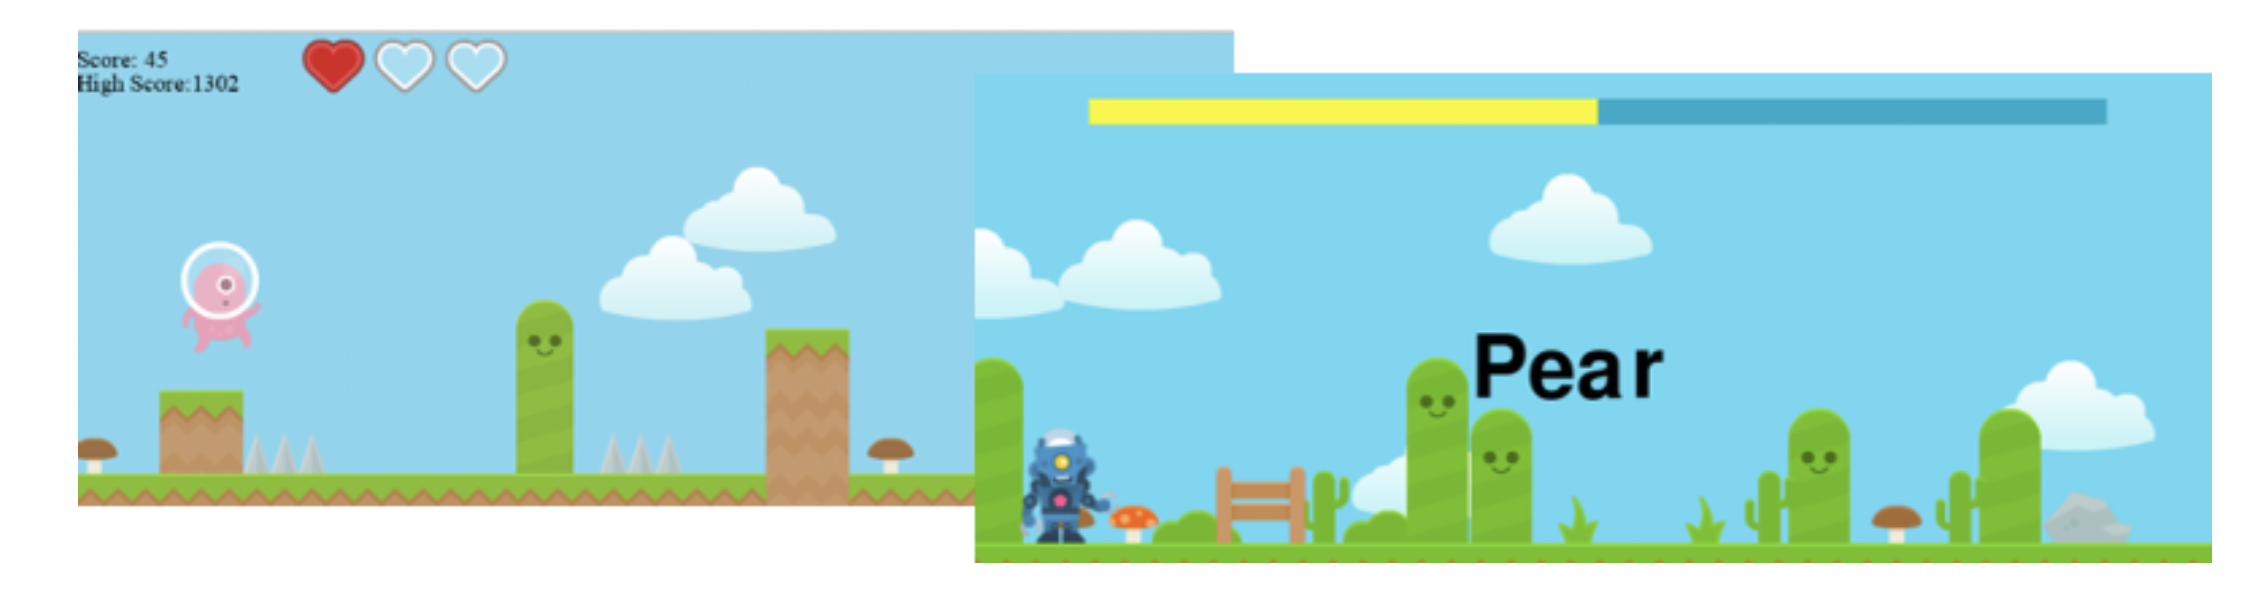
\includegraphics[width=1\textwidth]{imgs/exampleSLT.png}
    \caption{Illustrated herein are some examples of children's Speech and Language Technology applications that were developed during the course of this thesis. On the left, it is a running platformer game, where the user's voice controls the character. Pitch dictates running and jumping actions, while energy modulates the velocity of these actions. On the right, a reading task game is depicted, wherein a robot instructs the user to read designated words.}
    \label{fig:exSLT}

\end{figure}

% SLT could be the beginning of the answer and is already used in real life
In this context, \ac{SLT} have emerged as highly pertinent within the domain of speech therapy \cite{mendoza2022added}. These technologies encompass a spectrum of computational tools designed to analyse, understand and provide objective and precise automated assessments. Another benefit lies in their potential integration into gamification frameworks, thereby augmenting children's involvement during therapy \cite{brewer2013using}. Moreover, the ability to record speech utter by the patient during a session using \ac{SLT} enables post-session thorough analysis and long-term monitoring by the therapist. Due to the aforementioned reasons, the development of such tools has gained considerable attention, empowering patients to engage in exercises beyond therapy sessions, notably in a home setting. Some \ac{SLT} examples developed within the scope of the first stages of this thesis are illustrated in Figure \ref{fig:exSLT}.

\section{Problem statement}
% Technologies are more and more present
Recent years have seen increased integration of \ac{SLT} into various aspects of our daily lives, impacting a wide range of environments, including homes, transportation, education, and even the military. Noteworthy examples encompass voice assistants, hands-free computing, healthcare systems, automatic helplines, and speech-to-speech translation services. The performance progress in these applications was made possible through the use of machine learning techniques, especially deep learning approaches, the increasing computational capacities of our devices, and the ever-growing volume of data available to train and improve these systems.

% Children are a good target audience for SLT
Children represent a promising target audience for \ac{SLT} due to the inherent complexities of conventional computer interfaces, which pose challenges for them and limit their capacity to fully benefit from digital platforms. Indeed, children commonly face difficulties in manipulating mouse and keyboard inputs. Additionally, the abstract nature of traditional man-machine interfaces can impede the understanding necessary for effective interaction. In this context, speech-based systems emerge as a promising alternative, offering a more natural and accessible means for children to interact with technology. Through the use of speech recognition technologies, these speech systems mitigate the barriers associated with conventional interfaces, providing a fluid and intuitive interaction paradigm that aligns more closely with the developmental stages and cognitive abilities of young users. Another potential application of \ac{SLT} for children could be in the development of automatic reading tutors. Given that the process of learning to read is individual and varies for each child, a personalised automatic reading tutor could assist in tailoring the learning experience to the specific needs of each student. This has the potential to reduce the workload on teachers and provide additional support in the crucial skill of reading acquisition. Finally, the growing presence of voice assistants in home settings underscores the importance of reliable \ac{ASR} for children. In this context, a reliable ASR system becomes crucial to ensure a positive and effective user experience of seamless interaction with voice-enabled devices in various home environments.

% Automatic tools for speech therapy
As previously mentioned, \ac{SLT} applications are gradually making their way into the field of atypical speech, particularly for children. While these automatic tools are currently in their early stages and have limitations, there is indeed a rising interest in implementing atypical speech and language therapy systems with a focus on assisting \acp{SLP}. In this context, systems capable of automatically recognising speech content, assessing pronunciation quality and automatically detecting speech pathologies could be highly valuable in supporting pediatric \acp{SLP} and patients.

All of these objectives require the implementation of a robust \ac{ASR} system specifically tailored for healthy children, serving as a foundational model. Nevertheless, while speech recognition technologies for adult speakers have made substantial advancements, leading to increased accuracy, the performance of \ac{ASR} systems for children remains underperforming in comparison. This discrepancy results in unreliable systems for children and, by extension, their use in \ac{SLT} applications. This diminished performances can be attributed to a combination of factors, including intra- and inter-speaker variability, limited linguistic and phonetic knowledge, and the scarcity of available data.

% In this work we propose....
In this thesis, we will undertake a comprehensive investigation into the intricacies of children's speech, closely examining the inherent differences between children and adults in the domain of \ac{ASR}. Through this examination, the objective is to analyse the constraints associated with the application of adult-based systems to children's speech and, subsequently, to outline the methodologies present in the literature for enhancing \ac{ASR} systems. The overarching goal of this thesis is to establish a robust foundational system that effectively addresses the recognition of children's speech.

% Explain that there is no Pathological speech dataset
Initially, the context of this thesis aimed at addressing pathological speech for children. However, due to constraints in data availability, specifically the absence of a meaningful pathological children's speech dataset, experiments related to pathological speech in children were not included in this thesis. 
The shift in focus towards improving \ac{ASR} for healthy children was motivated by the importance of establishing a solid \ac{ASR} foundational system focusing on children. This shift broadens the potential applications of our research, ranging from personal assistants, automatic reading tutors and voice interactions with computer interfaces. Despite the pivot towards healthy children's speech, during the course of this thesis investigations into adult pathological speech have been conducted and are reported as part of this document in Annexe \ref{chapter:appendixA}.


% Research question
Our work toward improving automatic speech recognition for children specifically aims to answer the following research questions:
\begin{enumerate} 
\item Which knowledge transfer approach is best for efficiently modelling and improving traditional automatic recognition of children's speech? Can these approaches be used to efficiently exploit low-resource children's speech data from multiple languages?
\item  Can we furhter improve full end-to-end model fine-tuning of children \ac{ASR} by adapting part of the model? Particularly, what are the most important components to fine-tune?
%\item Is it possible to develop a parameter-efficient automatic speech recognition model for children? Can we further improve the parameter efficiency with other architectures? 

\item Does parameter efficient transfer improve children \ac{ASR} compared to full model fine-tuning? Which is the best approach for children parameter efficient \ac{ASR}? Can we propose a novel method that achieve state-of-the-art with fewer parameters? 

\item What is the impact of using children's synthetic speech to extend the amount of real children's data during training? How can we reduce the mismatch between real and synthetic data? Can we control the quality and speakers’ variability of the synthetic utterances?
\end{enumerate}

\section{Contributions}
% State of the art exploration
This thesis commenced with a comprehensive exploration of the current state-of-the-art in children's Automatic Speech Recognition (\ac{ASR}). We present an examination of the fundamental determinants that contribute to the decline in \ac{ASR} performance for children's speech. Additionally, we meticulously assess current research on children's speech. The primary aim was to identify potential avenues for improvement throughout the course of this thesis. 

%HMM-DNN contribution
Subsequent to the literature review, we start our research by the implementation of \ac{HMM-DNN} models for children \ac{ASR}. We explored different strategies to reduce the gap observed between children and adults in the context of both English and European Portuguese speech. We identified the effectiveness of knowledge transfer methods, specifically, transfer learning and multi-task learning. Transfer learning adapts speech recognition adult models by fine-tuning their weights for children's speech. On the other hand, multi-task learning exposed models to both adult and children's speech datasets simultaneously during training. In an innovative approach, we proposed to combine transfer learning and multi-task learning into a unified approach, the multi-task transfer learning framework. We applied this approach to multiple low-resource children's datasets from diverse language sources, which resulted in a publication at LREC 2022 and will be presented in Chapter \ref{chap:Chapter3}:
\begin{itemize}
    \item \textbf{Rolland, Thomas}, Alberto Abad, Catia Cucchiarini, and Helmer Strik. "Multilingual Transfer Learning for Children Automatic Speech Recognition." \textit{ Language Resources and Evaluation Conference} (2022).
\end{itemize}

% End-to-End contribution
Thereafter, our research turned into the end-to-end paradigm, motivated by the encouraging improvements observed in the end-to-end children's \ac{ASR} performance. We introduced a novel detailed transfer learning approach, called ``Partial fine-tuning", where our objective was to gain a thorough understanding of the specific components within the end-to-end architecture that significantly contributed to the remarkable improvements in recognition scores. The publication of the ``Partial fine-tunning" approach is still in preparation for submission and will be  presented in Chapter \ref{chap:4}:

\begin{itemize}
    \item \textbf{Rolland Thomas} and Alberto Abad. "Fine-tuning for children’s automatic speech recognition, are we doing it right? Introduction to Partial fine-tuning" \textit{In preparation for submission} (2024).
\end{itemize}


The identification of the most relevant components allowed the development of specific algorithms aimed at further improving the model's recognition performances. Particularly, we explored the integration of an additional set of parameters, the Adapters, directly into the original \ac{ASR} model. This integration facilitated a parameter-efficient approach to adapt the model, accepted at ICASSP 2024 and presented in Chapter \ref{chap:4}:

\begin{itemize}
    \item \textbf{Rolland Thomas} and Alberto Abad. "Exploring adapters with conformers for children’s automatic speech recognition." \textit{ International Conference on Acoustics, Speech and Signal Processing} (2024).
\end{itemize}

% TTS contribution
In response to the scarcity of large children's speech datasets, we delved into the exploration of leveraging synthetic speech to augment the existing dataset. However, our investigation revealed that a mismatch between real and synthetic data hindered the results. To address this challenge, we introduced additional processing steps to efficiently incorporate synthetic data. We proposed a double-way approach, wherein the synthetic data underwent an additional set of parameters. More detailed about this approach will be presented in Chapter \ref{chap:6}. This innovative methodology contributed to an enhanced \ac{ASR} system tailored for children and was published at ICASSP 2024:

\begin{itemize}
    \item \textbf{Rolland Thomas} and Alberto Abad. "Improved children’s automatic speech recognition combining adapters and synthetic data augmentation." \textit{International Conference on Acoustics, Speech and Signal Processing} (2024).
\end{itemize}

Finally, with the different successes achieved by parameter efficient strategies presented thorough this thesis, we evaluated Adapters to alternative approaches present in the literature. Furthermore, we introduced a novel parameter efficient transfer learning leveraging the redundancy present in Transformer-based architecture to significantly reduce the amount of parameters needed during training while preserving the accuracy, the ``Shared-Adapter". This work is detailed in Chapter \ref{chap:7} of this thesis and is currently in preparation for submission:
\begin{itemize}
    \item \textbf{Rolland Thomas} and Alberto Abad. "Shared-Adapter, leveraging Transformer-based redundancy for better parameter efficiency for children automatic speech recognition" \textit{In preparation for submission} (2024).
\end{itemize}

% Pathology dectection contributation
In tandem with the primary focus of enhancing children's \ac{ASR}, this thesis extends its scope to the detection of pathologies directly from speech. This secondary investigation retains relevance within the broader context of the thesis, particularly as we initially aimed to address the specific needs of children with pathological speech. We explored the use of embedding extracted from pre-trained models for the detection of different pathologies such as Alzheimer's disease, Parkinson's disease, obstructive sleep apnea and COVID-19, all presented in Annexe \ref{chapter:appendixA}:

\begin{itemize}
    \item Anna Pompili, \textbf{Thomas Rolland}, and Alberto Abad. "The INESC-ID multi-modal system for the ADReSS 2020 challenge." \textit{Interspeech} (2020).
    \item Catarina Botelho, Francisco Teixeira, \textbf{Thomas Rolland}, Alberto Abad, and Isabel Trancoso. "Pathological speech detection using x-vector embeddings." \textit{arXiv preprint} arXiv:2003.00864 (2020).
    \item Rubén Solera-Ureña, Catarina Botelho, Francisco Teixeira, \textbf{Thomas Rolland}, Alberto Abad, and Isabel Trancoso. "Transfer Learning-Based Cough Representations for Automatic Detection of COVID-19." \textit{Interspeech} (2021).
\end{itemize}


\section{Structure for the thesis}
The structure of this thesis comprises eight chapters. In Chapter \ref{chap:Chapter2}, we first introduce the challenges associated with automatic children's speech recognition. This chapter also provides an overview of the automatic speech recognition systems, along with an examination of the latest approaches specifically tailored to address the unique challenges posed by children's \ac{ASR}. Furthermore, a compilation of children's speech corpora is presented.

Following, in Chapter \ref{chap:Chapter3}, we present our work on the hybrid speech recognition paradigm, focusing on the evaluation of different knowledge transfer approaches and their combinations. In Chapter \ref{chap:4}, we shift towards the end-to-end paradigm, evaluating the role of the different components of the \ac{ASR} model during transfer learning and proposing our partial fine-tuning procedure. Subsequently, in Chapter \ref{chap:5}, we validate the use of Adapters as a parameter-efficient knowledge transfer approach for children's \ac{ASR}. In Chapter \ref{chap:6}, we build upon this knowledge to propose a novel approach to use imperfect synthetic data as data augmentation during transfer learning.
Next, in Chapter \ref{chap:7}, we investigate possible alternative approaches for parameter-efficient transfer learning, introducing a novel method using a shared Adapter across the different layers of the model. Finally, in Chapter \ref{chap:8}, we conclude the thesis with a summary of the different works and results studied in this thesis, as well as some perspectives of future work. 
% If Printing on DOUBLE SIDED pages, the second page should be white.
% Otherwise, comment the following command:
\cleardoublepage{}
%
%Chapter 2
%\fancychapter{Background - Children automatic speech recognition}
\label{chap:Chapter2}
\cleardoublepage
% General ASR
\ac{ASR}, or \ac{STT} refers to the process of mapping a raw spoken audio utterance into its corresponding text. 
The potential use of \ac{STT} applications across diverse fields has motivated the need for robust and reliable \ac{ASR} systems. These applications extend across various sectors, encompassing academia, medicine, industry, and the military. Notably, \ac{ASR} has made significant progress in recent years, thanks to the attention and investment from both industry and public authorities. This support has resulted in the deployment of applications such as voice assistants, hands-free interfaces, medical assistance, live translation, and more, all of which are widely used and accepted today.
%ASR work well on typical speech
Nowadays, the majority of \ac{ASR} applications are mainly developed and optimised for adult speech. Demonstrating high performance in conditions close to those encountered during the training phase. This focus on adult speech is explained by the immediate potential of \ac{ASR} applications for this target audience. In addition, training \ac{STT} models on adult speech has both advantages of data availability and relatively stable aspects of adult speech characteristics making the training easier. Indeed, adult speech is often more standardised, with established linguistic conventions and stable features.
However, the challenge arises when such systems are applied to recognise speech in mismatched scenarios, like atypical speech such as accented, pathological or children's speech. For example, in the context of children's speech, \ac{ASR} algorithms often exhibit a decline in performances, frequently two to five times worse \cite{childrenSpeechWorse}. In this context of children, this difference in performance can be mostly attributed to the intra- and inter-speaker variability. In fact, speech serves as a channel not only for linguistic content but also for paralinguistic cues that reveal aspects of the speaker's identity, including age, gender, state of health, emotional state and regional origin. Although this additional layer of information is highly valuable for human-to-human communication, it introduces a new level of complexity, making the development of a reliable \ac{ASR} system more challenging \cite{li2023asr}.
Furthermore, several external factors further negatively impact the performance, including noise, speaker variability, mispronunciation, and the quality of the recording \cite{li2014overview,king2017robust}.


% Children applications 
The potential applications of \ac{STT} in education and entertainment have led to a growing interest in \ac{ASR} for children. Indeed, children represent a demographic group that could well benefit from such applications for a number of reasons. Firstly, the complexity of traditional computer interfaces, such as keyboards and mice, can pose problems for young children, making speech interfaces a more accessible and user-friendly option. Secondly, speech and language applications, including reading tutors and speech and language acquisition assistants, promise to address educational inequalities among children and facilitate their integration into society by giving them personalised and tailored attention.

In this chapter, we first present the various challenges associated with children's speech recognition. These challenges encompass the unique characteristics of children's speech, including high acoustic and linguistic variability, as well as the limited amount of labelled data available for training. Then, we provide a brief introduction to \ac{ASR}, tracing its historical development from early pattern recognition approaches to the advent of statistical models and the contemporary move towards end-to-end models. This historical background provides an understanding of the underlying principles behind \ac{ASR} technologies. Subsequently, we review the state-of-the-art methods specifically designed to address the challenges posed by children's \ac{ASR}.  The aim of this in-depth exploration is to provide a clear overview of the different techniques that are being used to improve children's speech recognition. Finally, the chapter concludes with a discussion that synthesises the different perspectives presented earlier and the ones selected for this thesis.

\section{Children speech  recognition challenges}%----------------------------------- ~3 pages
\label{section:Children_seepch_challenges}
% Intro on how children speech is different from adult
In this section, we explore the distinct challenges posed by children's speech to \ac{ASR} systems. In particular, we will explore the main differences with adult speech.  Indeed, the divergences between child and adult speech are mainly due to the continuous growth and intellectual development of children. This growth has direct repercussions on automatic speech recognition scores. In order to present the different challenges associated with \ac{ASR} for children, we have identified at least three of the main factors that degrade recognition performance.
First, we examine the acoustic variability of children's speech. The acoustic characteristics of children's speech differ considerably from those of adults due to factors such as vocal tract size, pitch modulation and articulatory differences. These variations represent a significant challenge for speech recognition systems, which are often trained on adult speech datasets and have never encountered such variations. Taking this acoustic variability into account becomes imperative for the development of accurate and robust \ac{ASR} models adapted to the unique characteristics of children's speech.
Next, we will present the linguistic and phonetic knowledge inherent in children. Indeed, children's language evolves dynamically over time, with vocabulary expansion, phonetic development and language mastery. This linguistic evolution also raises challenges for \ac{ASR} systems, as they need to be robust to age-specific linguistic variation and imprecise pronunciation. In a similar way as the acoustic variability, effective modelling of these linguistic variabilities is important for children's speech recognition.
Finally, we present the challenge posed by the limited availability of corpora of children's speech. Unlike adult speech, data corpora containing labelled examples of children's speech are relatively rare and small in size. This scarcity constrains the training of robust \ac{ASR} models, as it limits their exposure to the various linguistic and acoustic variations of children's speech.

% Introduce the three following sections
\subsection{Speech variability}%**************************************************************
% Define Speech, especially adult 
Speech production is a complex process involving the synchronised actions and collaboration of several elements of the speech production apparatus. These include the vocal cords, tongue, lips and mouth. The coordination of these elements leads to fluctuations in air pressure, producing a wave called speech. Speech is therefore essentially a measure of air pressure over time. The waveforms of human speech encompass a range of frequency components from 20 \ac{Hz} to 20 kHz. These are detected and processed by the auditory system and the human brain. Because speech is based on frequency components, an accurate understanding of these frequency components, such as fundamental frequency and formant frequencies, is essential for the development of reliable speech processing tools.

% F0
The fundamental frequency, often called F0, plays a crucial role in the analysis of speech signals. It characterises the (quasi-) periodic average oscillations produced by the vibrations of the vocal folds. Measured in \ac{Hz}, F0 is often considered to be the acoustic correlate of pitch. F0 shows an inverse relationship with the vibrating mass of the vocal cords, leading to distinct F0 values for different demographic groups. As a general rule, adult males have lower F0 values, ranging from around 100 to 150 \ac{Hz}. Women, on the other hand, tend to have higher F0 values, generally between 200 and 300 \ac{Hz}. Children, whose vocal cords are smaller, often have even higher F0 values, generally ranging from 300 to 450 \ac{Hz}. These variations in F0 contribute to the perceptual differences in pitch between individuals of different ages and genders. 
% F0 changes from children to adult
According to \cite{Acoustic_change_children}, significant differences in F0 between male and female speakers generally appear from the age of 12. For male speakers, decreases in F0 were observed on average between the ages of 11 and 15, at the time of puberty, and did not change significantly after the age of 15. Furthermore, it was observed that the relatively large variation between male subjects at the ages of 13 and 14 also implies that the starting point of puberty varies among speakers in these age groups. For female speakers, the pitch drops between the ages of 7 and 12, and there is no significant change in pitch after this age. In addition, the change in F0 in female subjects is more gradual as compared to male speakers.

It is essential to emphasise that F0 is not a static parameter; on the contrary, it exhibits continuous variation within a sentence. This dynamic nature allows F0 to be used expressively in speech, conveying nuances such as accent, emotion and intonation patterns. Variations in F0 help to distinguish between different types of speech acts, such as statements, questions and exclamations.

%Formants
A formant frequency refers to a concentration of acoustic energy centred around a specific frequency in a speech waveform. As defined by the Acoustical Society of America, it is \textit{``a range of frequencies in which there is an absolute or relative maximum in the sound spectrum. The frequency at the maximum is the formant frequency"}. Formants play a crucial role in characterising vowel sounds and distinguishing between them. In speech analysis, the first three formants, known as F1, F2 and F3, are commonly used for their importance in capturing the acoustic characteristics of vowels and their contribution to the timbre of speech sounds.


% Children frequency shift
The pioneering study by Peterson and Barney in 1952 \cite{first_vowel_study} marked a turning point in the exploration of the formant components of vowels, particularly in the context of children's speech. Researchers undertook a comparative analysis, examining the vowel frequencies of children and comparing them with those of adult men and women. This research was the first to show significant variations in vowel frequencies based on the speaker's age and gender. Building upon this foundational work, subsequent studies \cite{reviewASRchildren,Acoustic_change_children,why_children_speech_no_working} have provided further insights into the acoustic characteristics of children's speech. These investigations have consistently demonstrated a correlation between acoustics and children's age, attributing these variations primarily to the growth of the children's vocal apparatus. The scaling behaviour of formant frequencies with respect to age is shown in Figure \ref{fig:f1f2_children}. Here, the evolving vowel space, defined by four reference vowels (\textit{/IY/,/AE/,/AA/} and \textit{/UW/}) linearly decreases with age and aligns with the adult level around the age of 15. Additionally, as highlighted in \cite{reviewASRchildren}, the vowel space becomes more compact as age increases, indicative of a downward trend in the dynamic range of formant values. These variations and age-related differences emphasise the critical challenge of inter-speaker variability, especially for young children.


\begin{figure}[ht]
\centering
\subfigure[Changes in F1-F2 vowel space as a function of age]{\label{fig:f1f2_children}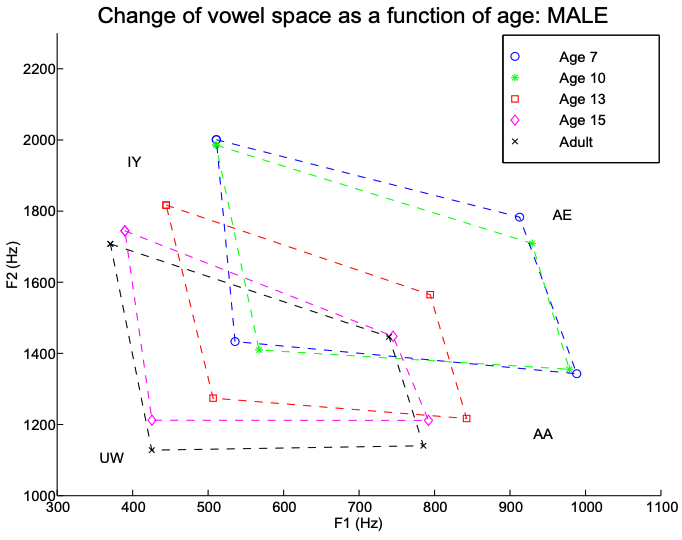
\includegraphics[width=0.48\textwidth]{imgs/f1f2children.png}}
\subfigure[Mean cepstral distance between the two repetitions of the same vowels]{\label{fig:intra_children}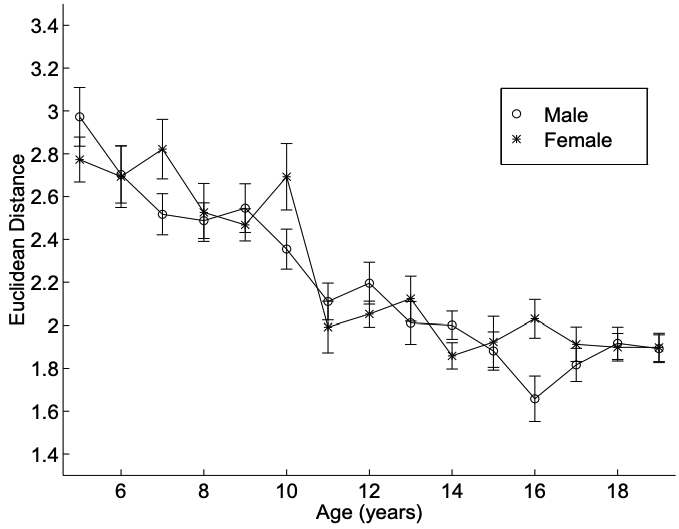
\includegraphics[width=0.48\textwidth]{imgs/intraspeakervariability.png}}
\caption{Formant and cepstral variability. Figures taken from \cite{reviewASRchildren}}
\end{figure}

\begin{figure}[ht]
\centering
\subfigure[Averaged-vowel duration across all vowels and subjects in each age group]{\label{fig:duration_vowel_children}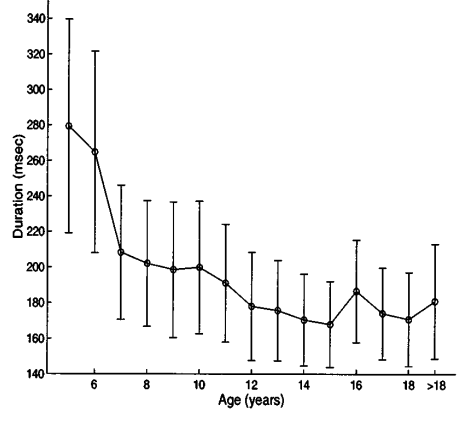
\includegraphics[width=0.48\textwidth]{imgs/children_vowel_duration.png}}
\subfigure[Within- and between-subject variations. The between-subject variation is reduced by a factor of 2.0]{\label{fig:intra_duration_children}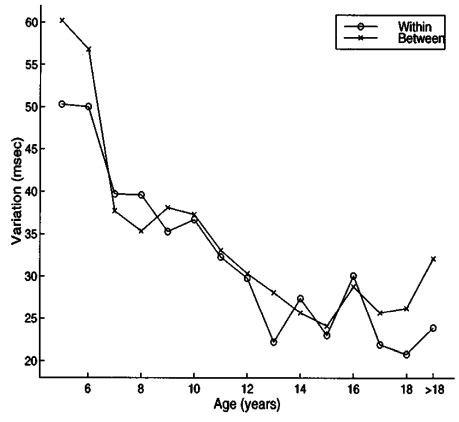
\includegraphics[width=0.48\textwidth]{imgs/Intra_inter_duration.png}}
\caption{Segmental duration variability. Figures taken from \cite{Acoustic_change_children}}
\end{figure}


In addition to inter-speaker variability, \cite{Acoustic_change_children} also highlight the fact that children's speech also exhibits intra-speaker variability, signifying that the speech produced by the same individual can exhibit variations. This variability arises from two primary sources. Firstly, as previously discussed, the acoustic characteristics of children can significantly differ at different ages due to the ongoing growth of their vocal apparatus.  Secondly, even at the same age, the same child may produce variable speech, even when articulating the same vowel. As depicted in Figure \ref{fig:intra_children}, the average cepstral distance between two repetitions of the same vowels by the same child tends to decrease with age, particularly after the age of 10. This reduction in intra-speaker variability is attributed to the progressive mastery of speech articulation components as children grow and mature their motor skills abilities. The decrease in cepstral distance suggests a more coherent and standardised articulation of vowels over time.

% Duration segments for children are longer
Segmental duration is another important aspect of human speech. A segment, as defined by Crystal \cite{segment_definition}, is: \textit{``Any discrete unit that can be identified, either physically or auditorily, in the stream of speech"}. These segmental durations could be of vowel or sentence duration. Vowel duration, in particular, is of significant importance in vowel discrimination. Research, as presented in \cite{Acoustic_change_children}, investigates how these characteristics change in children's speech. As demonstrated in Figure \ref{fig:duration_vowel_children}, the average vowel duration in children exhibits variations with age. On average, younger children tend to have longer vowel durations, resulting in a slower speaking rate. However, as children become more comfortable with the processes of speech production with age, vowel duration gradually decreases. Similarly to children frequency variations, segmental duration exhibits intra-speaker variability, as illustrated in Figure \ref{fig:intra_duration_children}.


% Conclusion on frequency challenges 
In conclusion, dealing with both intra- and inter-speaker variability in children's speech, particularly in those under the age of 15, poses a substantial challenge for developing high-performance speech processing models. Especially, this challenge is exacerbated in the context of children's \ac{ASR} where the age of the child is often unknown. In addition, the dynamic processes of the vocal tract growth, changes in linguistic knowledge and the maturation of control of speech apparatus occur simultaneously and overlap, making it considerably more challenging to accurately disentangle and model their effects. The intricate nature of children's speech, marked by intra and inter-speaker variations, underscores the necessity for sophisticated and adaptive models that can accommodate the unique characteristics of these speakers.



\subsection{Language and phonetic knowledge} %************************************************
\label{subsection:mispron}
% Intro on language and phonetic
Language is a complex and multifaceted system of communication that involves the use of symbols, such as words to convey meaning. It is a unique human ability and serves as a fundamental aspect of human cognition and social interactions. Linguists have identified five basic components of language \cite{moats2000speech}, including phonology (sounds), morphology (structure and construction of words), semantics (meaning), syntax (grammar and sentence structure), and pragmatics (how language is used in context). It allows individuals to express thoughts, share information, and engage in social interactions. It is important to note that, languages vary across cultures and regions, exhibiting a rich diversity of sounds, structures, and expressions. Additionally, language can be spoken, written, or signed, and evolves over time. For children, the mastery of language is a crucial milestone in their cognitive development. Furthermore, language plays a central role in shaping culture, identity, and the transmission of knowledge to them. The children's ability to use language develops with age, achieving adult capabilities around the age of 13, as indicated by \cite{Acoustic_change_children}. This progression enables the children to transition from producing simple sounds and words to generating more complex sounds and fully articulated sentences.

% Explain what are the main disfluency
During the process of language acquisition, children, constrained by their limited linguistic knowledge, often make pronunciation errors and encounter disfluencies \cite{language_children}. According to \cite{clark1977psychology}, these errors may include a variety of phenomena, such as:
\begin{itemize}
    \item \textbf{Substitution}:  Involves the inadvertent replacement of the correct pronunciation of an entire word with an alternative word.
    \item \textbf{Omission}:  Refers to the act of leaving out or neglecting a part of speech, a word, or a phrase that would typically be included in a grammatically correct or complete sentence.
    \item \textbf{Mispronunciation}:  Involves the act of pronouncing a part of a word incorrectly, deviating from the standard or expected pronunciation of this word.
    \item \textbf{Pause and Hesitation}: Entails temporary breaks or delays in speech during which a speaker might refrain from producing sound or articulate speech in a hesitant manner.
    \item \textbf{Filler and mumbling}:  Filler encompasses linguistic elements used during pauses or hesitations when a speaker needs time to think, including unintelligible sounds, words, or phrases without significant meaning. Mumbling is characterised by unclear or indistinct speech, often marked by low volume, unclear articulation, and imprecise pronunciation.
    \item \textbf{False-start}:  Refers to an instance where a speaker begins a sentence or a word and then stops abruptly before completing it. This interruption is often followed by a restart or a correction to articulate the intended message more accurately.
    \item \textbf{Sound-out}: Involves a pronunciation strategy in which a speaker articulates a word by pronouncing each sound or phoneme separately, rather than blending them together seamlessly.
\end{itemize}

% Give more example of disfluency over age
Potamianos and Narayanan's study \cite{language_children2} revealed significant insights into the variability and characteristics of children's linguistics. They found that inter-speaker variability is approximately twice as much as intra-speaker variability. Additionally, their research found that the rate of mispronunciations is twice as high for children aged 8 to 10 compared to those aged 11 to 14. Conversely, the trend is reversed for filler and pauses, where the older group exhibits a higher rate. Furthermore, younger children, of 8 to 10 years, tend to produce more false-starts and breathing.

% Explain that it is hard to model, that adaptation from adult because Children has different grammatical constructs 
In adult speech, pronunciation errors and disfluencies are also present, but their occurrences are typically lower than what is observed in the speech of children, as supported by studies such as \cite{Children_language_model,children_language_model2}. In addition, these studies used language models specifically trained on children's speech, demonstrating their advantages over the use of adult language models. These findings underscored the differences between children's and adults's linguistics, encompassing variations in grammatical structures as well as the presence of mispronunciations and disfluencies. Such insights are crucial for the development of effective language models tailored to the unique characteristics of children.


\subsection{Data scarcity}%****************************************************************
\label{section:data_scarcity}
% Data is key in this deep learning time
In recent years, the emergence of deep learning has brought significant advancements in the \ac{ASR} field. The combination of increased computational power and the availability of large datasets has played a pivotal role in these improvements. The success of deep learning is largely attributed to \ac{DNN}s, which can approximate complex non-linear functions. With the help of this capability, \ac{DNN} excels in capturing complex patterns and accurate representations of speech data. However, the efficacy of a \ac{DNN} in capturing speech patterns depends a lot on the availability of training data. Indeed, using large-size datasets is pivotal for enhancing the capabilities and generalisation of \ac{DNN}-based \ac{ASR} systems. Notably, top-performing \ac{ASR} systems like Whisper have been trained on exceptionally large datasets, surpassing 680,000 hours of data collected from the web \cite{radford2023robust}. There is a noticeable trend in the speech research community towards the collection of larger datasets, exemplified by initiatives such as the LibriSpeech dataset, which comprises around 1,000 hours of speech \cite{librispeech}, and the GigaSpeech dataset, featuring 10,000 hours of speech \cite{chen2021gigaspeech}.

% Explain pb with children dataset
Unfortunately, despite rare recent efforts to collect larger children datasets \cite{MyST,singakids,ahmed2021auskidtalk}, the majority of publicly available children corpora include fewer than fifty hours of speech. This is significantly less than a typical adult speech corpora, which usually contains hundreds or even thousands of hours of data. Furthermore, the majority of the accessible children's data are English corpus \cite{MyST,cmu,cslu,pf-star-british,ahmed2021auskidtalk}. However, English is a resource-rich pluricentric language which should be seen more as an exceptional case, rather than an average representative. A compilation of existing datasets containing children's speech will be presented in \ref{section:children_corpora}.

% Ethical problems
The scarcity of children's speech datasets availability can be partially attributed to a combination of ethical, legal, and technical challenges. Collecting speech data from children raises ethical concerns related to obtaining consent, ensuring privacy, and protecting minors. The heightened awareness of online safety and security concerns further complicates the creation and sharing of datasets that include children's speech, as there is a need to safeguard against potential misuse and ensure the anonymity of participants.
% Need of a diversity
Beyond ethical and legal considerations, technical challenges also play a role. Children's speech patterns, language development, and pronunciation can vary significantly across different age groups, as explained in previous sections, making it more challenging to create datasets that accurately represent the diversity of children's speech. Moreover, the resource-intensiveness of collecting high-quality speech data from children, which involves careful planning, recruitment efforts, and coordination with schools or parents, can further contribute to the limited availability of such datasets.
% age problem, school recording -> noise, attention span of the children
Finally, collecting speech data from children is a challenging and time-consuming task. Various factors can significantly impact the quality of the gathered speech. These include children's short attention spans, recording environments that might be noisy (such as classrooms), and the quality of the speech, which is highly dependent on the task at hand (reading tasks are generally more complex for children).

% explain that with data, a lot of problems can be solved
The importance of having a large database of children's speech to cover different variabilities has been emphasised in a study conducted by Liao in 2015 \cite{asr-google}. In this work, the researchers trained an \ac{ASR} model using a large in-house corpus of children's speech. Notably, this corpus was comparable in size to typical adult speech corpora. The result was the attainment of state-of-the-art performance by the \ac{ASR} model, even demonstrating competitiveness with adult speech recognition systems. This study underscores the crucial role of large-size and diverse children's speech datasets in developing robust and high-performance \ac{ASR} models tailored to the unique characteristics of children's speech.


\newpage
\section{Introduction to automatic speech recognition}%----------------------------------------------------------- ~11 pages
In this section, a brief historical overview of \ac{ASR} is presented, laying the foundation for a subsequent exploration of predominant trends and modules within \ac{ASR} systems. This comprehension is necessary for the following sections of this thesis. While not exhaustive, this overview provides essential insights, with certain topics falling beyond the scope of this thesis are intentionally omitted. For a more exhaustive understanding of \ac{ASR}, readers are encouraged to consult references such as \cite{benzeghiba2007automatic, karpagavalli2016review, arora2012automatic}. This section is structured as follows: Firstly, we present the historical evolution of \ac{ASR}, followed by a description of traditional HMM-based \ac{ASR} systems, succeeded by an explanation of the end-to-end paradigm. Concluding this section, a discussion on automatic speech recognition metrics is presented.

\subsection{A brief history of Automatic Speech Recognition}

\subsubsection{Early Days}

The origins of speech recognition technology can be traced back to the 1950s and 1960s, with initial projects focusing on isolated word recognition with a speaker-dependent system. One of the earliest projects in this direction was the creation of a digit recogniser at Bell Telephone Laboratories in 1952. This recogniser demonstrated the automatic recognition of telephone-quality digits spoken at normal speech rates by a single adult male speaker, achieving an impressive accuracy of up to 99\%. The system relied on formant frequency approximations to recognise entire words. It is important to underscore that within this recogniser, there was an absence of explicit modeling of syllables, consonants, vowels, or any other sub-word units. In this recogniser, a word was treated as a single unit, which was then compared with ten standard digit patterns to find the best match. The recognition process first involved extracting two frequency ranges, below and above 900 \ac{Hz}. Motivated by the observation that these two frequency ranges approximately align with the frequencies of the first two formants in speech. Then, these formant approximations were plotted on a 2D plot with a trace interruption period of 10ms. Finally, when presented with new audio, the system generated a new plot, compared it to the reference plots of the ten digits, and returned the closest match by computing the highest relative correlation coefficient. Figure \ref{Bell} illustrates an example of the 2D representation of the ten digits.


\begin{figure}[h]
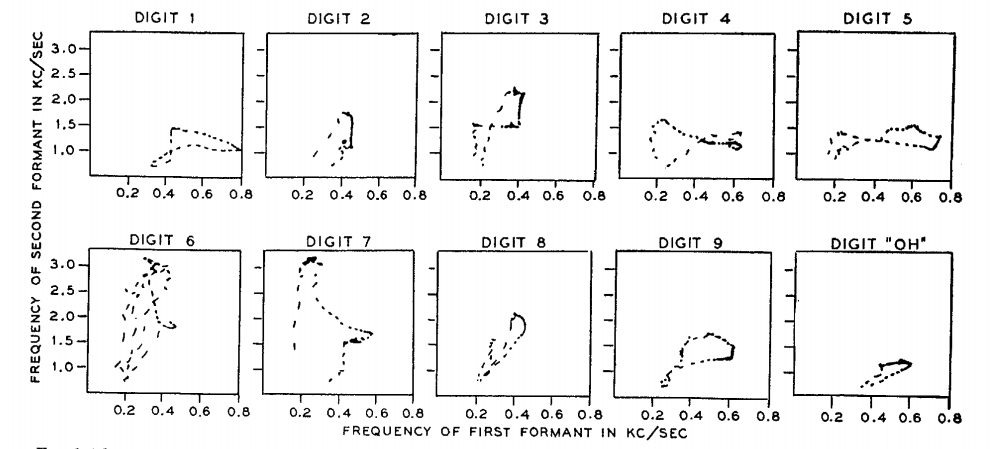
\includegraphics[width=\textwidth]{imgs/bell.png}
\caption{Example of a standard digit pattern from Davis et al. 1952}
\label{Bell}
\end{figure}


In 1962, IBM developed Shoebox, a device capable of recognising 16 spoken words, including the ten digits and command words such as ``plus," ``minus," and ``total." This system employed a similar pattern-matching algorithm to the one used in the Bell Telephone Laboratories's recogniser.


Nevertheless, extending such a system to a larger vocabulary would be impractical. Indeed, the template-matching approach necessitated saving each word representation on disk and comparing the unknown spoken word with all these representations. Therefore, when attempting to scale this approach to automatic large vocabulary recognition, issues of time and disk usage complexity emerged as a significant challenge. Furthermore, in order for the circuit to deliver an accuracy of the same range for a new speaker, a preliminary analysis of the speech of that individual and subsequent circuit adjustments were necessary. These limitations underscored the need for more scalable and adaptive approaches and led the field of automatic speech recognition to continue to evolve.



\subsubsection{The Speech Understanding Research program} 

In the early 1970s, subsequent to the initial success of pattern-matching algorithms in single-word recognition, the Advanced Research Program Agency of the U.S. Department of Defense, ARPA, initiated funding for a five-year program called \ac{SUR}. The overarching goal of \ac{SUR} was to ``obtain a breakthrough in speech understanding capability that could then be used toward the development of practical man-machine communication system". Within the context of this program, four distinct research groups were funded: two from \ac{CMU}, one from Bolt Beranek and Newman Inc. (BBN Hwim), and the last one from \ac{SDC}. Each group was assigned a specific task, such as dealing with facts about ships, travel budget management, and document retrieval. The ultimate objective for each group was to create a system capable of recognising simple sentences within the context of their assigned task, using a vocabulary of 1,000 words and achieving a \ac{WER} of 10\% in a reasonable amount of time.


The realisation that the pattern-matching word identification strategy could not be directly applied to the challenge of sentence understanding prompted a redesign of the single-word identification system. On the first hand, one key recognition was that the acoustic characteristics of words can vary considerably based on the context of the sentence. The impracticality of storing each word and all its possible different variations on disk became apparent. Moreover, determining the boundaries of each word was almost an impossible task, and even if these boundaries were identified, the pattern-matching computation, involving comparisons with each of the 1,000 stored words and all their possible variations, would be time-consuming and exceed the reasonable time requirement. Secondly, another crucial consideration in the redesign of the system was that the length of the spoken sentence is variable and unknown, in contrast to the relatively fixed length in single-word identification tasks.

To address these challenges, a shift was made to a smaller unit than the word for modelling speech -namely, phonemes. Phonemes are the smallest distinctive and meaningful units that compose speech. Each language is associated with a finite set of phonemes, typically fewer than 50, which can be combined to form words. This shift enabled a more efficient and flexible representation of speech, accommodating the variability in the pronunciation of words.

Among all the systems proposed in the project, the Harpy system implemented by Lowerre in 1976 by the \ac{CMU} team exhibited the best performances \cite{klatt1977review}. Harpy is a speaker-specific system that uses a pattern-matching algorithm at the phoneme level instead of the word level. The system employs a set of 98 phonemes and diphones a pair of consecutive phonemes-, encompassing pronunciations of all words, along with a graph compiling all accepted sentences using 15,000 states. When a new spoken utterance is provided to the system, it undergoes an initial processing phase, involving low-pass filtering at 5 k\ac{Hz}, digitisation at 10,000 samples per second, and computation of 14 linear prediction coefficients with a 10ms shift. To speed up the decoding process, analogous adjacent acoustic segments are grouped together. Subsequently, these audio segments are compared against the 98 phoneme templates, and the system deduces the optimal path over the decoding graph. Figure \ref{harpy} provides an example of a decoding graph in the Harpy system.


\begin{figure}[h]
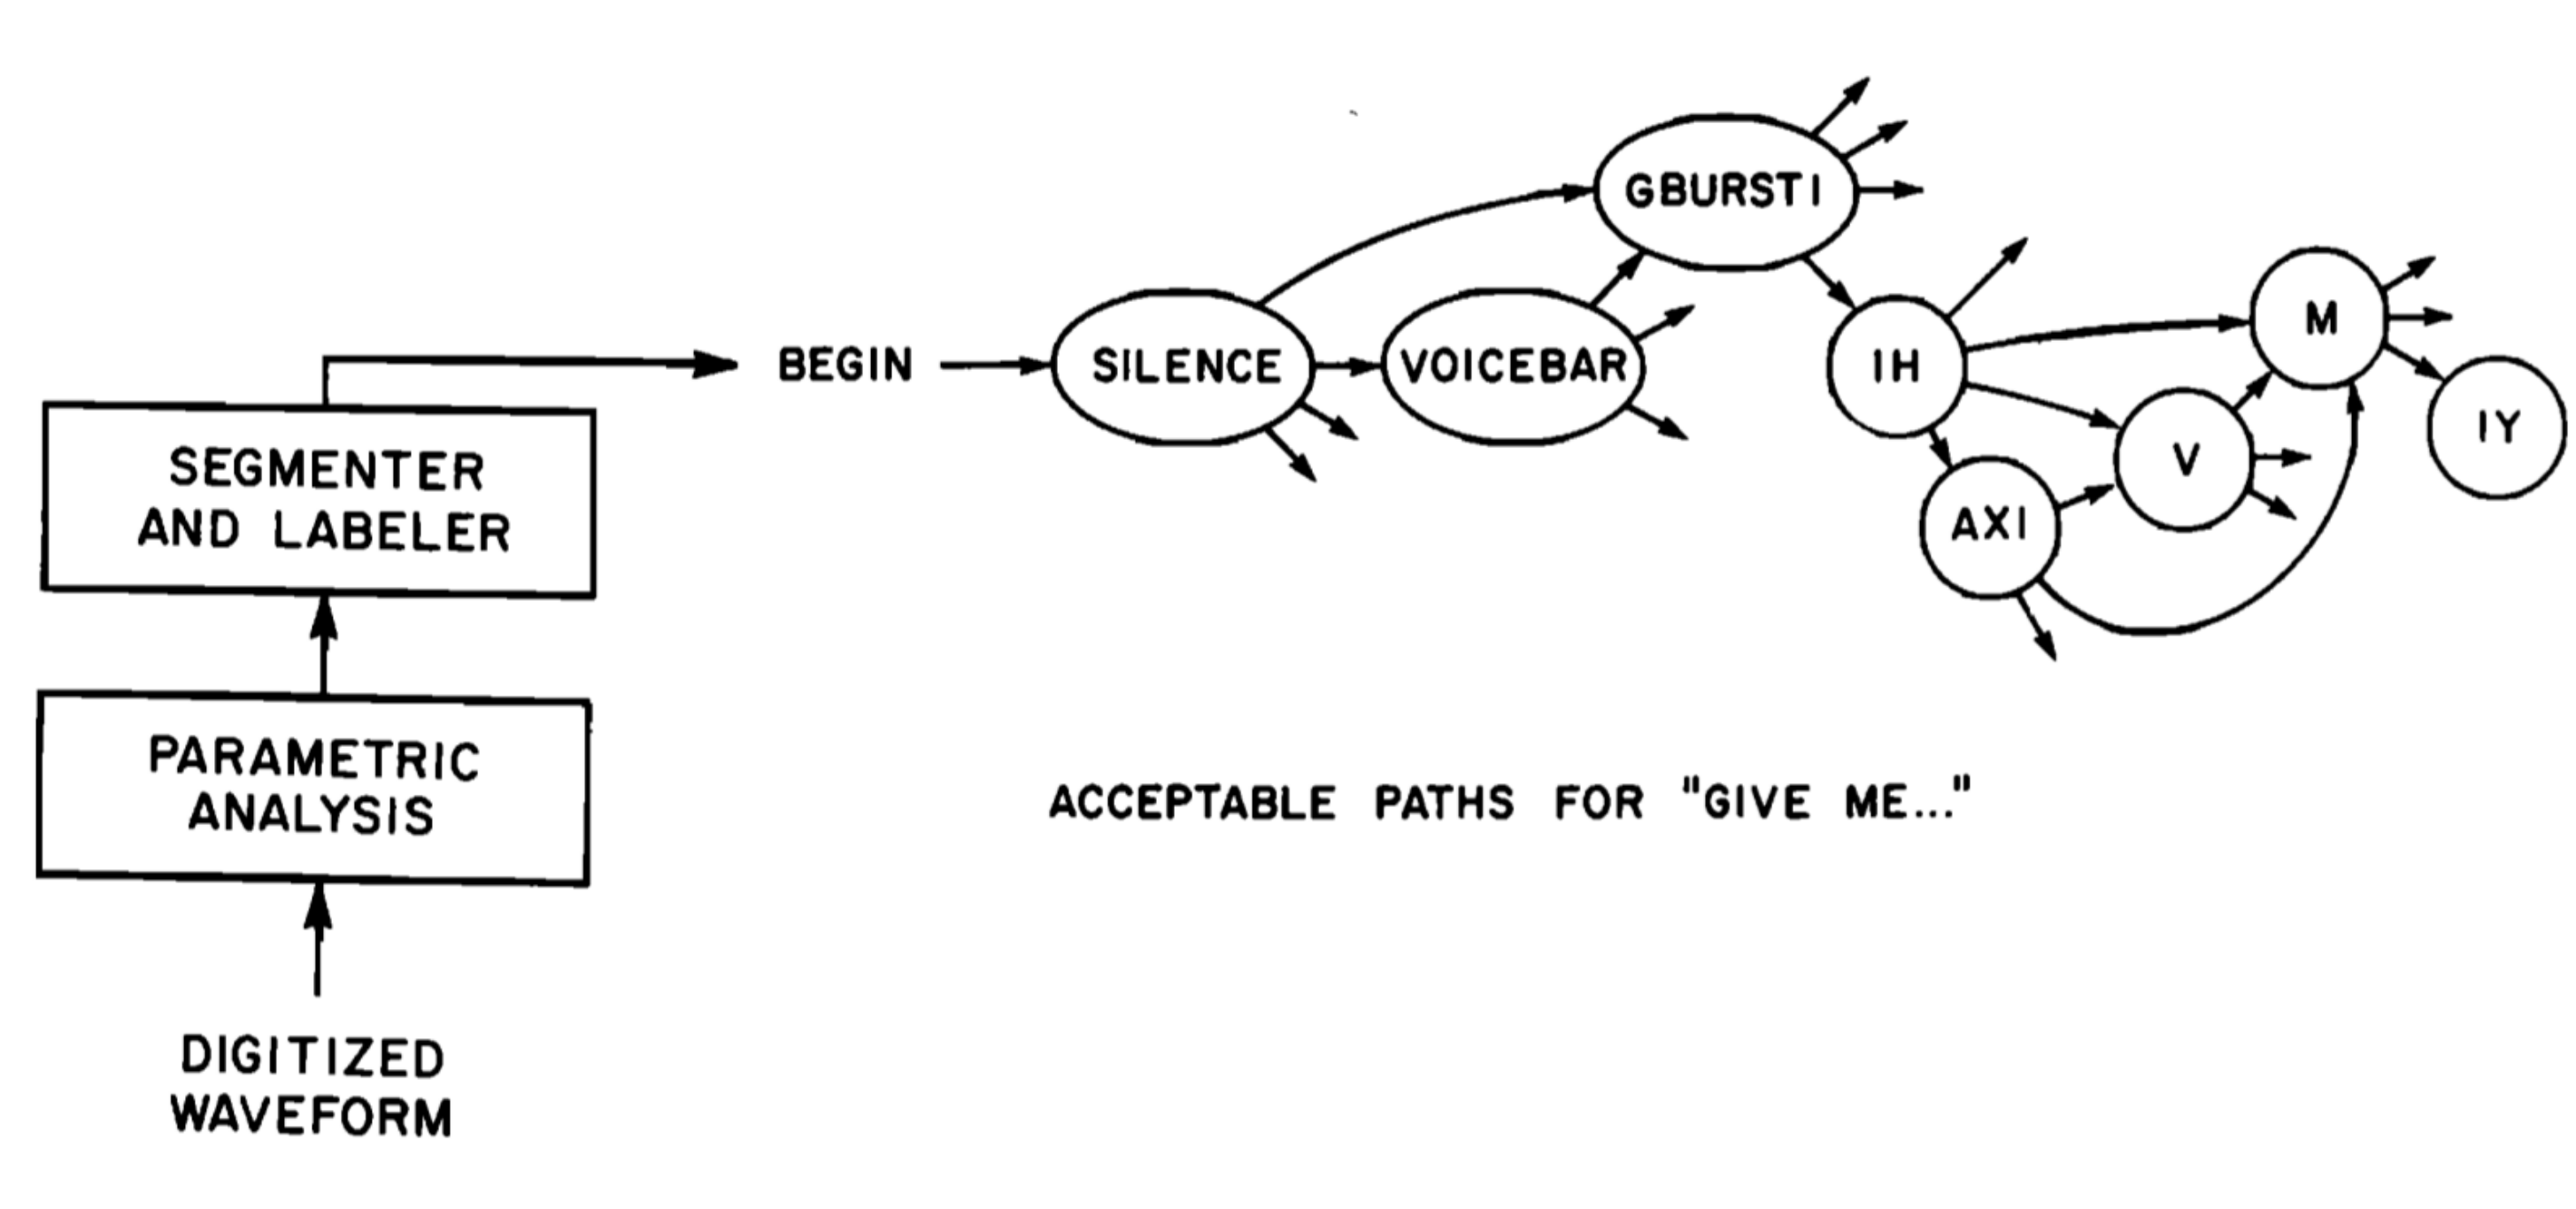
\includegraphics[width=\textwidth]{imgs/harpy.png}
\caption{Example of a decoding graph in the Harpy system for the sentence ``GIVE ME" from \cite{klatt1977review}}
\label{harpy}
\end{figure}

Notwithstanding the achievements and success of the Harpy system, it has limitations that hinder its broader applicability. As a speaker-specific system, it requires tuning for each new speaker over the 98 phoneme templates. Additionally, the system is constrained to recognise a vocabulary of no more than 1,000 words and relies on simple handcrafted grammar, making it less reliable for handling spontaneous speech. Moreover, the decoding time of the system falls short of real-time requirements. These constraints highlight the need for more generalisable and efficient speech recognition systems, especially for handling diverse speakers and spontaneous speech scenarios. Therefore, as research progressed, the limitations of pattern-matching-based approaches became apparent. This realisation prompted the exploration of probabilistic modelling techniques, marking a shift towards more sophisticated and adaptable approaches in \ac{ASR}. 


\subsection{Traditional automatic speech recognition systems} % ~4 pages %************************
% HMM-DNN
\begin{figure}

\includegraphics[width=\textwidth]{imgs/HMM-GMM_architecture.png}
\caption{Architecture of a HMM-based speech recognition system}
\label{HMM-GMM-model}
\end{figure}

%What are HMM
In the 1970s, the introduction of \acp{HMM} led to a paradigm shift in \ac{ASR} research, moving away from traditional pattern-matching methods towards statistical modelling \cite{first_asr}. Indeed, \acp{HMM} are particularly effective at capturing the sequential and temporal nature of speech. They assume that speech can be represented as a sequence of hidden states, each state corresponding to a distinct phonetic unit. \ac{HMM} models the transitions between these states and, at each state, generates observable acoustic features. The hidden aspect refers to the fact that the underlying states are not directly observed but inferred from the observable features. \acp{HMM} are particularly well suited to modelling speech dynamics, as they can represent the variability of speech sounds over time. In the context of \ac{ASR}, \acp{HMM} have been widely used to model phonemes, words or sub-word units.

%What are GMM
Building on this foundation, the 1980s saw the emergence of \acp{GMM}, which further enhanced the statistical modelling capabilities of \ac{ASR} \cite{htk_book}. \acp{GMM} allowed for a more flexible representation of the probability distributions underlying speech features.
\acp{GMM} are used to model the statistical distribution of acoustic features associated with each hidden state in an \ac{HMM}. Commonly, a system that uses both \ac{HMM} and \ac{GMM} is referred to as a \ac{HMM-GMM} framework. By using \ac{GMM}, they assume that the distribution of features can be approximated by a mixture of several Gaussian distributions. \ac{GMM} are versatile in capturing the variability of speech sounds, allowing a more flexible representation of the acoustic units. In \ac{ASR}, \acp{GMM} are commonly used to model the emission probabilities associated with each state in an \ac{HMM}. This means that given a particular state, the \ac{GMM} provides the likelihood of observing a specific set of acoustic features. By combining the temporal modelling capabilities of \acp{HMM} with the statistical representation power of \acp{GMM}, this framework effectively captures the complex relationship between acoustic features and phonetic units.

% What are statistical grammars
Finally, in the 1990s, statistical grammar also played a crucial role, providing a structured framework for incorporating linguistic information into \ac{ASR} systems \cite{darpa1992}. Statistical grammars represent a category of grammars that integrate statistical information to characterise the probability of diverse linguistic structures. In contrast to traditional rule-based grammars, which articulate a language's syntax through explicit rules, statistical grammars adopt a data-driven methodology. They assign probabilities to various linguistic constructions based on observed frequencies within a designated corpus.

%What are DNN
The components illustrated in Figure \ref{HMM-GMM-model} represent the traditional \ac{ASR} pipeline. To this day, these components continue to form the core of modern \ac{HMM}-based \ac{ASR} systems. However, the recent evolution in the \ac{ASR} field has been marked by a significant shift from the \ac{GMM} to the adoption of \ac{DNN}. Driven by \ac{DNN} ability to effectively model complex patterns and hierarchies in speech data, \acp{DNN} have demonstrated superior performance, contributing to enhanced accuracy and efficiency in speech recognition systems \cite{hmm-dnn}. Called hybrid models, or \ac{HMM-DNN}, by effectively combining both the strengths of \acp{HMM} and \acp{DNN}. A \ac{DNN} is a subtype of artificial neural networks consisting of multiple layers of interconnected neurons. These neurons, organised in layers, receive an input signal, and each connection between neurons is characterised by a weight that signifies its strength. In addition, each neuron is associated with a bias weight, providing an additional learnable parameter. During training, the network adjusts these weights and biases to minimise the difference between predicted and actual outputs, a process known as backpropagation. Moreover, a non-linear activation function is placed within neurons, as it enables the network to model intricate, non-linear patterns of the data. The weights, biases and non-linearity allow \acp{DNN} to capture complex relationships and representations from the data, learning hierarchical features and abstracting information across multiple layers of the network.

%Math formulation
In this statistical framework, the continuous speech audio waveform is transformed into a sequence of fixed-size acoustic vectors, denoted as $\boldsymbol{X}=x_1,...,x_T$. The goal of the \ac{ASR} system is to determine the sequence of words, $\boldsymbol{w}=w_1,...,w_L$, that is most likely to have produced the observed acoustic vector sequence $\boldsymbol{X}$. This is formulated as finding the word sequence $\hat{w}$ that maximises the conditional probability $P(\boldsymbol{w}|X)$. More formally:

\begin{equation} \label{equation:asr_0}
    \boldsymbol{\hat{w}} = \argmax_{\boldsymbol{w}} \{P(\boldsymbol{w}|X)\}
\end{equation}
However, directly modelling the conditional probability $P(\boldsymbol{w}|X)$ can be challenging. Bayes' Rule offers a way to express this probability in terms of more manageable components, specifically by decomposing it into the product of the likelihood of the observed acoustic vector sequence given the word sequence $P(X|\boldsymbol{w})$ and the prior probability of the word sequence $P(\boldsymbol{w})$. Therefore, equation \ref{equation:asr_0} became:
\begin{equation}  \label{equation:asr}
    \hat{\boldsymbol{w}} = \argmax_{\boldsymbol{w}} \{\frac{P(X|\boldsymbol{w})P(\boldsymbol{w})}{P(X)}\} =\argmax_{\boldsymbol{w}} \{P(X|\boldsymbol{w})P(\boldsymbol{w})\}
\end{equation}
Here, the likelihood $P(\boldsymbol{X}|\boldsymbol{w})$ is determined by the acoustic model component, capturing the probability of observing the acoustic vector sequence $\boldsymbol{X}$ given the word sequence $\boldsymbol{w}$. In parallel, the prior probability $P(\boldsymbol{w})$ is determined by the language model component. The term $P(X)$ is not essential for determining the maximum probability and can be omitted in the context of finding the most likely word sequence. Subsequent sections will provide a more in-depth exploration of these distinct components and their processes.


% Feature extraction 
\subsubsection{Feature extraction}%*********************************************************
\label{subsection:features}
The first step in the \ac{STT} pipeline, as depicted in Figure \ref{HMM-GMM-model}, is the feature extraction from the speech signal.
The feature extraction component plays a crucial role in capturing pertinent information about the linguistic content of speech. In addition, the efficacy of speech recognition systems is intricately tied to the quality of the extracted features.
%THOMAS: As shown in Annex B?
To this end, for each time step, the continuous waveform is transformed into a small fixed-size vector. An acceptable assumption is that speech is considered stationary within the time span covered by a single vector. Consequently, feature vectors are typically computed at intervals of 10 milliseconds, often with a 25-millisecond overlapping window.

\begin{figure}
    \begin{center}
    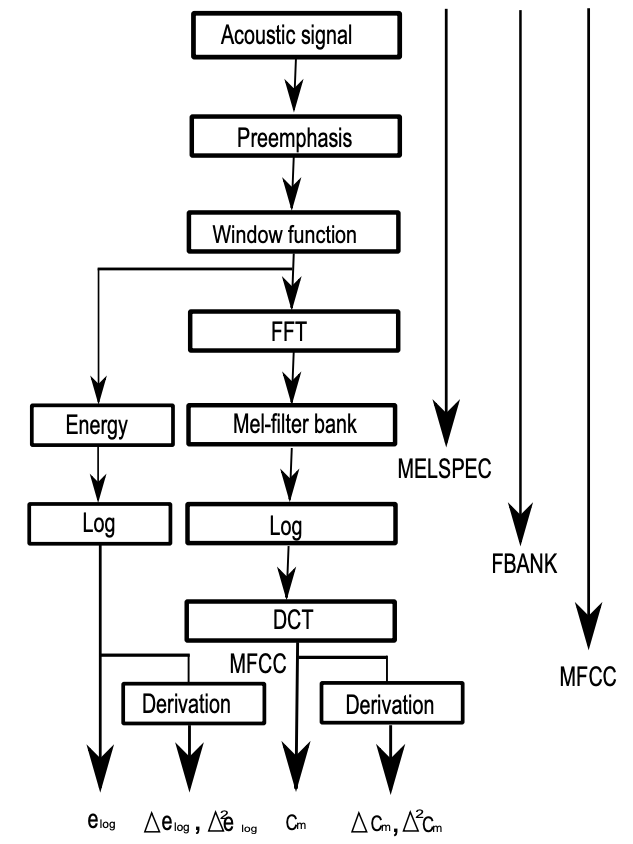
\includegraphics[scale=0.3]{imgs/features.png}
    \caption{Principal block scheme of extraction of main speech features for ASR: Melspec, fbanks and MFCC coefficients from \cite{kiktova2013comparison}}
    \label{feature_block}    
    \end{center}
\end{figure}

% MFCC
Within the domain of \ac{ASR}, a broad range of different acoustic features can be employed. However, in the context of \ac{HMM}-based models, the predominant features encompass  \ac{PLP}, Melspec, \ac{fbanks}, and\ac{MFCC}. Particularly, \acp{MFCC} as introduced by Davis and Mermelstein \cite{mfcc}, stand as the predominant features in \ac{HMM-GMM} and \ac{HMM-DNN} architectures.
The process of extracting \acp{MFCC} typically involves several steps to capture essential information from the speech signal. First, a preemphasis filter is applied to the signal. Subsequently, the signal is segmented into frames, and a Hamming window with a duration of 25 milliseconds is applied to each frame. The frames are then transformed into the frequency domain using the discrete \ac{FFT}, resulting in a magnitude spectrum.
The next stage involves passing the magnitude spectrum through a bank of triangular-shaped filters. Extracting features at this point yields melspec features. The energy output from each filter is log-compressed, concluding the extraction process at this stage would result in \ac{fbanks} features. Finally, \acp{MFCC} are obtained by transforming the filterbank features into the cepstral domain using the \ac{DCT} to decorrelate the energies obtained from the filterbanks. The overall representation of this extraction process is illustrated in Figure \ref{feature_block}.


%Delta features and concatenation
To incorporate information about the dynamics of the speech signal, the feature vector for each time step is augmented with the first and second-order derivatives, commonly denoted as $\Delta$ (Delta) and $\Delta\Delta$ (Delta-Delta), respectively. The first-order derivative coefficients, often referred to as $\Delta$ coefficients, are calculated by taking the difference between consecutive feature vectors. Mathematically, the $\Delta$ coefficients for a feature vector at time $t$ are computed as follows:
\begin{equation}
 \label{equation:delta}
    \Delta_i = \frac{\sum^{N}_{n=1}n(f_{i+n} - f_{i-n})}{2 \sum^N_{n=1}n^2} \\
\end{equation}
Here, $f_i$ represents the feature at the instant $i$.Typically, $n$ is set to 2, indicating that the first-order derivatives are calculated by considering the differences between the feature at the current time $t$ and its neighbouring features at $t \pm 2$. The $\Delta\Delta$ coefficients, also written $\Delta^2$, represent the second-order derivatives and are computed in a similar manner as $\Delta$ in equation \ref{equation:delta} by taking the difference between consecutive $\Delta$ coefficients instead of the spectral feature $f$. The concatenation of the first-order derivative ($\Delta$) and second-order derivative ($\Delta^2$) features with the spectral features is denoted as $x_i$. Mathematically, this concatenation can be expressed as follows:

\begin{align}
    \boldsymbol{x_i} = [f_i \qquad \Delta_i \qquad \Delta^{2}_i]
\end{align}
Here, $f_i$ represents the spectral feature at the instant $i$, $\Delta_i$ represents the first-order derivative feature at the same instant, and $\Delta^2_i$ represents the second-order derivative feature at the same instant. The resulting feature vector $x_i$ encapsulates information about the spectral content of the speech signal as well as its temporal dynamics, providing a more comprehensive representation for subsequent processing by the \ac{ASR} system, especially the acoustic model.


% What is an Acoustic model
\subsubsection{Acoustic model}%****************************************************************
% There role and limitation of simple AM
The role of the \ac{AM} is to determine $P(\boldsymbol{X}|\boldsymbol{w})$. While employing a classifier such as \ac{GMM} models with one \ac{GMM} per phone is a straightforward approach, it tends to disregard the temporal dependencies inherent in speech, such as co-articulation. Indeed, accurately categorising each frame necessitates the consideration of not only the current frame but also its context, encompassing both previous and following frames. Additionally, there are acoustic differences at the beginning, middle, and end of each phone, which further complicate the classification task. To address these concerns, the \ac{HMM} framework has been proposed as a solution \cite{Dragon_system}. \acp{HMM} offer temporal flexibility, incorporating concepts such as self-looping, and provide a well-understood framework with effective learning (Expectation Maximisation) and decoding (Viterbi) algorithms. 


\begin{figure}
    \begin{center}
    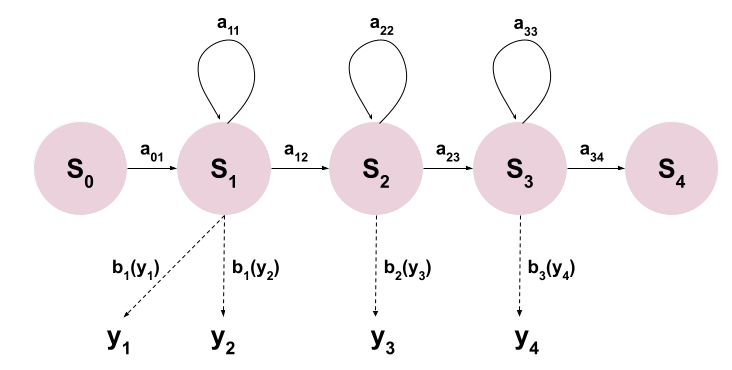
\includegraphics[scale=0.3]{imgs/HMM_monophone.png}
    \caption{Three-state Hidden Markov Model for modelling phones}
    \label{HMM_monophone}    
    \end{center}
\end{figure}
% Use of HMM and HMM-GMM
In the \ac{HMM} terminology, the observed variables, denoted as $y_i$, correspond to the acoustic features (e.g., speech signal), while the hidden variables are represented as states, denoted as $s_i$. The states are generated using a first-order Markov process, where the $i^{th}$ state $s_i$ depends solely on the previous state $s_{i-1}$. The transition from one state to another is determined by the transition probability $a_{ij}$. Upon entering a state $s_i$, an observation in the form of an acoustic vector is emitted, and this emission is modelled by the distribution $b_i(\cdot)$ associated with that state. Typically, this emission distribution is modelled by a \ac{GMM}. It is assumed that all observations are independent given the states that generated them. A fundamental \ac{HMM} configuration for speech recognition, represented in Figure \ref{HMM_monophone}, involves a three-state model representing the beginning, middle, and end of a phoneme, along with an initial and final state. This model, known as a monophone \ac{HMM-GMM}, constitutes a basic unit for phonetic modelling. For example, since English has 44 phonemes \cite{bizzocchi2017many}, a monophone system in English will have 44 separate \ac{HMM-GMM}. However, due to the influence of co-articulation effects and the desire to capture phonetic variations based on context, more complex models, such as triphone systems, are employed \cite{schwartz1985context}. A triphone system aims to model each phoneme in its specific phonetic context, leading to a significantly larger number of required models.  Indeed, for a language with $N$ phonemes, there should be $N^3$ models to train. For example, in English, which has 44 phonemes, the total number of models would be  $44 * 44 * 44$ resulting in 85,184 models. To manage the computational complexity, these models are often clustered using decision trees \cite{bahl1991context}. This hierarchical clustering helps capture phonetic variations efficiently while working with limited available data.

% HMM-DNN
The concept of hybrid models gained prominence in the 1990s with the integration of \ac{MLP} as replacements for \acp{GMM} in the \ac{HMM-GMM} system \cite{bourlard2012connectionist,meinedo2003audimus}. Subsequently, the introduction of \acp{DNN}, which are basically \acp{MLP} with a large number of hidden layers, in 2012 marked a significant advancement in various \ac{ASR} tasks \cite{hmm-dnn}. The efficacy of \acp{DNN} lies in their capability to capture complex and highly non-linear relationships between inputs (e.g., audio features) and outputs (e.g., phoneme labels) due to the substantial number of parameters induced by the deep architecture.

However, the training of \ac{HMM-DNN} and \ac{HMM-GMM} models differs. Neural networks necessitate labelled data for training, which includes both input features and corresponding output labels (e.g., phoneme labels). Standard speech training data often lacks this detailed labelling, providing only audio waveforms and utterance transcriptions. Consequently, the training of \ac{HMM-DNN} models relies on alignments generated by an \ac{HMM-GMM}. Typically, the training process of \ac{HMM-DNN} involves initial flat-start monophone training with \ac{HMM-GMM}, followed by iterative steps into triphone training with more precise alignments and subsequently the \ac{DNN} training. In consequence, the precision of the \ac{HMM-GMM} alignment directly impacts the efficacy of \ac{DNN} model training. As \ac{ASR} continues to advance, the integration of various \ac{DNN} architectures, including \acp{CNN} \cite{lang1990time}, \acp{LSTM} networks \cite{sak2014long}, and \acp{TDNN} \cite{waibel2013phoneme}, further refines the modelling of spatial and temporal relationships, laying the foundation for more sophisticated and context-aware speech recognition systems.

\subsubsection{Pronunciation model} %******************************************************
The pronunciation model in \ac{ASR}, often referred to as a dictionary or lexicon, plays a crucial role in establishing the correspondence between phonetic units, such as phonemes, and the respective words in the language. Indeed, words are essentially comprised of phonetic segments, and the pronunciation model specifies how these segments combine to articulate the pronunciation of each word. It is noteworthy that a single word may have multiple pronunciations. This mapping takes the form of an entry where all possible words are associated with their corresponding sequence of phones. Examples of words along with their corresponding phonetic sequences are illustrated in Table \ref{CMU_DICT}. Traditionally, this mapping is obtained manually, relying on phonetic and linguistic knowledge. 

Furthermore, the integration of statistical \ac{G2P} tools \cite{g2p} augments the lexicon by facilitating the generation of pronunciations for words that may not be explicitly included in the dictionary.

\begin{figure}
    \begin{minipage}[t]{0.5\textwidth}
        \centering
        \begin{tabular}{ccc}
            \hline
            Phoneme & Example & Translation \\
            \hline
            AA & odd & AA D \\
            AE & at & AE T \\
            AH & hut & HH AH T \\
            AO & ought & AO T \\
            AW & cow & K AW \\
            AY & hide & HH AY D \\
            B & be & B IY \\
            CH & cheese & CH IY Z \\
            D & dee & D IY \\
            DH & thee & DH IY \\
            EH & Ed & EH D \\
            ER & hurt & HH ER T \\
            EY & ate & EY T \\
            F & fee & F IY \\
            G & green & G R IY N \\
            HH & he & HH IY \\
            IH & it & IH T \\
            IY & eat & IY T \\
            JH & gee & JH IY \\
            K & key & K IY \\
            \hline
        \end{tabular}
    \end{minipage}%
    \begin{minipage}[t]{0.5\textwidth}
        \centering
        \begin{tabular}{ccc}
            \hline
            Phoneme & Example & Translation \\
            \hline
            L & lee & L IY \\
            M & me & M IY \\
            N & knee & N IY \\
            NG & ping & P IH NG \\
            OW & oat & OW T \\
            OY & toy & T OY \\
            P & pee & P IY \\
            R & read & R IY D \\
            S & sea & S IY \\
            SH & she & SH IY \\
            T & tea & T IY \\
            TH & theta & TH EY T AH \\
            UH & hood & HH UH D \\
            UW & two & T UW \\
            V & vee & V IY \\
            W & we & W IY \\
            Y & yield & Y IY L D \\
            Z & zee & Z IY \\
            ZH & seizure & S IY ZH ER \\
            \hline
        \end{tabular}
    \end{minipage}
    \caption{Phoneme set and examples of CMU dictionary using 39 phonemes from \cite{weide1998carnegie}}
    \label{CMU_DICT}
\end{figure}


\subsubsection{Language model}%****************************************************************
% Role of language model
The \ac{LM}, often referred to as grammar, holds a pivotal role in \ac{ASR}, responsible for determining the probability $P(\boldsymbol{w})$ of equation \ref{equation:asr}. Beyond its use in \ac{ASR}, the applications of language models extend into diverse fields including \ac{NLP} \cite{n-grams-NLP}, computational biology  \cite{n-grams-computational_biology}, and data compression \cite{n-gram-compression}. The two most successful approaches to language modelling widely adopted in \ac{ASR} are, respectively, statistical methods and models based on deep learning. 


% N-grams
Statistical \acp{LM} rely on traditional techniques like \ac{HMM} and N-grams. Particularly, N-grams, are the simplest approach for language modelling, they estimate the likelihood of the next word based on the context of the preceding $n$ words as follows:
\begin{equation}
    P(\boldsymbol{w})= P(w_1 , w_2 ,\dots,w_L)  =\prod_{i=1}^L P(w_i| w_{i-n} , \dots,w_{i-1}  )
\end{equation}
The level of context can vary from the case of $n=1$ -the 1-gram -or unigram- which considers each word independently to higher-order $n$-grams that incorporate more extensive context for enhanced accuracy. The unigram model would be defined as follows:
\begin{equation}
    P(\boldsymbol{w})=P(w_1, w_2,\dots,w_L )  = \prod_{i=1}^L P(w_i)
\end{equation}
Despite the evident advantages of employing a larger $n$ for enhanced contextual information in language modelling, practical considerations and computational limitations often impose constraints on the choice of $n$ in real-world \ac{ASR} applications. The escalating combinational complexity associated with higher $n$ values becomes computationally demanding, presenting challenges for efficient processing, storage, and training. As a result, the majority of \ac{ASR} applications typically use trigrams or 4-grams, striking a balance between contextual accuracy and computational feasibility.

Furthermore, determining the start of sequence probability precisely introduces intricacies, especially with larger $n$-grams. Additionally, the reliance on training data poses a notable limitation for $n$-grams, particularly in estimating the likelihood of unseen words. This deficiency becomes apparent when facing vocabulary expansion or encountering out-of-vocabulary terms, necessitating specific techniques such as smoothing to address these challenges.\cite{n-grams-smoothing}.

% Deep learning based LM
In contrast, deep learning-based \acp{LM} has opened up a new era, employing neural networks with complex architectures to achieve remarkable modelling capabilities. Unlike traditional n-grams, these models demonstrate a high degree of flexibility, and ease training and do not require as many resources as n-grams to be efficient. Recent advances in language modelling, exemplified by state-of-the-art models such as \ac{BERT} \cite{Bert} or \ac{GPT} \cite{brown2020language}, are built on deep learning networks.


A key factor contributing to the success of deep-learning language models is the incorporation of attention mechanisms. Unlike the limited contextual awareness of n-grams, attention mechanisms allocate varying degrees of importance to different words within a sentence. This approach enables the model to focus more on crucial elements, capturing intricate dependencies and semantic information that contribute to a more accurate language representation. The attention mechanism's ability to discern and prioritise important words enhances the overall performance and effectiveness of deep-learning language models.


\subsubsection{Decoder}%**********************************************************************

In the context of \ac{ASR}, the decoder role is to use the language, acoustic, and pronunciation models to determine the most likely word sequence, denoted as $\boldsymbol{\hat{w}}$, given a corresponding sequence of acoustic features, denoted as $\boldsymbol{Y}$ (as referred in equation \ref{equation:asr_0}). This is achieved by employing dynamic programming to search through all potential sequences. Notably, the Viterbi algorithm \cite{viterbi_decoder} is instrumental in efficiently solving this decoding problem. However, in practical applications, a direct implementation of the Viterbi algorithm could become challenging, especially for continuous speech, where considerations such as model topology, language model constraints, and computational constraints must be taken into account. N-gram language models and cross-word triphone contexts further complicate the search space. To address these challenges, various approaches have emerged. 

One approach involves constraining the search space by maintaining multiple hypotheses in parallel \cite{valtchev1994novel} or dynamically expanding it as the search progresses \cite{aubert1995large}. Another alternative is to use beam search where the idea is to prune search paths which are unlikely to succeed. More recently, recent advancements in \ac{WFST} technology offer a comprehensive solution by integrating all necessary information, including acoustic models, pronunciation, and language model probabilities, into a single, highly optimised network \cite{mohri1997finite,caseiro2002using}. This approach provides both flexibility and efficiency, making it a valuable tool for \ac{ASR}. As demonstrated by the Kaldi speech recognition toolkit \cite{kaldi}, it stands out as a widely adopted toolkit that leverages \acp{WFST} for decoding. 

Although decoders are primarily designed to find the best solution to the aforementioned probability computation in equation \ref{equation:asr_0}, they can also generate a set of the N-best hypotheses. This capability enables multiple passes over the data without incurring the computational expense of repeatedly solving the probability computation from scratch. The word lattice \cite{richardson1995lattice} serves as a convenient structure for storing these hypotheses, consisting of nodes representing points in time and spanning arcs representing word hypotheses.
Word lattices offer remarkable flexibility, allowing for rescoring by using them as input recognition networks. Furthermore, they can be expanded to facilitate rescoring by a higher-order language model.


\newpage
\subsection{End-to-end automatic speech recognition} % 1-2 pages%*********************
\label{section:SOTAE2E}
\begin{figure}
    \centering
    
\includegraphics[width=\textwidth]{imgs/End2End_architeccture.png}
    \caption{Architecture of an end-to-end speech recognition system}
    \label{fig:e2e_archi}
\end{figure}
% Intro on E2E
End-to-end speech recognition represents a paradigm shift in the field, presenting a streamlined and holistic approach compared to traditional \acp{HMM}-based systems. In contrast to conventional modular systems that incorporate distinct acoustic, pronunciation, and language models, end-to-end architectures aim to simplify the \ac{ASR} process by directly mapping input audio signals to transcriptions within a single neural network model as illustrated in \ref{fig:e2e_archi}. Indeed, one of the key disadvantages of hybrid models is the factorised training of all modules independently, which can lead to error accumulation and mismatches between the different components. Therefore end-to-end strategy simplifies the overall system design, eliminating the requirement for pre-aligned training data and post-processing of outputs, thereby fostering a more data-driven and automatic learning process.
In this paradigm, word-level transcriptions are transformed into character-level transcriptions. Considering the sequence of fixed-size acoustic vectors $\boldsymbol{X}=x_1,...,x_T$ and the corresponding character sequence $\boldsymbol{Y}=y_1,...,y_N$, where $T$ and $N$ represent the numbers of frames and the length of the character sequence respectively, the objective of end-to-end models is to learn the conditional probability of the character $y_i$ given the input $\boldsymbol{X}$ and the preceding output $y_{<i}$:

\begin{equation}
     P(Y|X) = \prod_{i=1}^{N}P(y_i | X,y_{<i})
 \end{equation}

 In recent years, with the growing interest in the end-to-end \ac{ASR} paradigm, these systems have demonstrated increasing performances. Particularly, in scenarios where a large amount of labelled training data is available. Recently, the use of end-to-end systems has allowed comparable or even superior performance compared to traditional \ac{HMM}-based systems across various \ac{ASR} datasets \cite{hannun2014deep,hmmvse2e}. However, despite its promising results, end-to-end speech recognition faces several challenges. Most importantly, these systems require a large corpus of training data to operate effectively. In the absence of such a corpus, the model may struggle to perform correctly \cite{hmm-end2end}. In addition, handling rare or out-of-vocabulary words remains a significant challenge. Finally, the generalisation across new acoustic conditions of the model can be an issue. Therefore, there is a need for research on end-to-end speech recognition, particularly to simplify the end-to-end design, training, and robustness of these speech recognition systems.
 
 The overall structure of end-to-end systems depicted in figure \ref{fig:e2e_archi} highlights the integration of the acoustic model, pronunciation model, and language model into a single neural network in end-to-end architectures. Nevertheless, the feature extraction stage remains identical to traditional \ac{ASR} systems. In end-to-end systems, the most commonly employed fixed-size acoustic features are filterbanks. Motivated by the higher flexibility that they provide and their capability of capturing relevant information from the speech signal compared to \acp{MFCC}.

 Transitioning to the end-to-end paradigm has necessitated the development of new training approaches. Indeed, training an end-to-end model differs significantly from training traditional \ac{HMM}-based systems. Notably, two training procedures have emerged in the literature of end-to-end \ac{ASR}: Connectionist Temporal Classification and sequence-to-sequence architectures. Each approach comes with its own distinct features and advantages, and the subsequent sections offer a more in-depth exploration of these two methodologies. It is worth mentioning that while these are distinct methods that can function independently, they can also be employed in conjunction.
 
 \subsubsection{Connectionist Temporal Classification}
 The first step towards end-to-end \ac{ASR} was made with the introduction of the \ac{CTC} objective function, by Grave et al. \cite{First_End2End}. The main innovation of \ac{CTC} is that it eliminates the need for pre-segmented training data, enabling the model to automatically learn the alignments between the $N$ input speech frame $\boldsymbol{X}$ and the output sequence of $T$ phones $\boldsymbol{Y}$ if $N \leq T$, representing a departure from the traditional HMM-based models.

 To this end, the \ac{CTC} objective function consists of two essential sub-processes: path probability calculation and path aggregation. Consider $\mathcal{V}$ as the set of possible paths of phone-label sequences of length $T$, and let $p^t_k$ denote the probability of observing the label $k$ at time $t$. It is noteworthy that \ac{CTC} necessitates the length of the label sequence $Y$ to be equal to $T$. To address any length difference between $N$ and $T$, a blank label ``-'' is introduced, representing the probability of observing no label. 
 
 First, the path probability calculation involves computing the conditional probability of any path $\pi \in \mathcal{V}$ given the observed acoustic features $\boldsymbol{X}$.Mathematically, this is expressed as:
 \begin{equation}
    p(\pi|X) = \prod_{t=1}^{T}p_{\pi_t}^{t} , \forall \pi \in \mathcal{V}
\end{equation}
 Where $\pi_t$ denotes the label at time $t$ in sequence path $\pi$. Considering all possible paths and their respective probabilities is crucial, but direct computation becomes infeasible due to the exponential number of potential paths.
 
 To address the computational challenges, the path aggregation step comes into play. Its purpose is to sum the probabilities of paths that correspond to the same label sequence $\boldsymbol{Y}$ by marginalising over all possible paths. The path aggregation also merge the same contiguous labels and deletes the blank label. For example, two different paths ``b-ii-r-d'' and ``b-i-r-dd'' become ``bird''. This is mathematically represented as:
\begin{equation}
    p(Y|X) = \sum_{\pi \in \theta_Y}p(\pi|X)
\end{equation}
Where $\theta_Y$ is a subset of $\mathcal{V}$ of all possible path $\pi$ corresponding, after aggregation, to the label sequence $Y$.

\subsubsection{Sequence to sequence}
%LAS attention mechanism and seq2seq
The \ac{Seq2Seq} architecture, initially proposed by Sutskever for machine translation \cite{sutskever2014sequence} stands as an important paradigm of end-to-end \ac{ASR} systems. The original context of its application was for machine translation tasks where word sequences were translated from one language to another. The inherent challenge lies in the differing lengths of input and output sequences. However, this architectural framework, especially with the integration of attention mechanisms \cite{bahdanau2014neural}, has showcased remarkable versatility, extending its efficacy across diverse applications such as image captioning \cite{seq2seq_imagecaption}, conversational modelling \cite{vinyals2015neural}, text summarisation \cite{nallapati2016abstractive}, and \ac{ASR} \cite{dong2018speech}.

The core components of a standard \ac{Seq2Seq} model consist of an Encoder and a Decoder modules. The Encoder processes input sequences of variable length, transforming them into a sequence of vectors often denoted as the ``internal state" or ``hidden representation". This sequence of vectors encapsulates the crucial information extracted from the input features. Subsequently, the Decoder uses this sequence of vector representation to generate an output sequence of tokens iteratively. Mathematically expressed as:
\begin{equation}
    p(y_1,...,y_T) = \prod_{i=1}^{T} p(y_i| y_0,...y_{i-1}, f(H))
\end{equation}
where $f(H)$ represents a function of the Encoder's output $H = (h_1, ..., h_N)$. Notably, in \ac{Seq2Seq} models incorporating attention mechanisms, $f(H)$ includes attention to selectively focus on relevant segments within $H$ for predicting the current target token. The \ac{Seq2Seq} objective function is formulated to train the model by maximising the conditional probability of generating the target sequence given the input sequence using \ac{NLL} loss or \ac{CE} loss.

A significant difference from \ac{CTC}-based models lies in the fact that \ac{Seq2Seq} models do not make independent assumptions about output labels. Instead, they directly model the conditional probability of each target token given the preceding tokens in the output sequence and the encoder's output. This end-to-end approach empowers \ac{Seq2Seq} models to handle sequences of varying lengths, making them particularly advantageous for speech recognition, where precise alignment between input and output is challenging.


\subsection{Automatic Speech Recognition metrics}%**********************************************************************
% What is WER
In the domain of \ac{ASR}, metrics serve as indispensable tools for assessing the accuracy and effectiveness of systems. These metrics provide quantitative evaluations that act as a crucial benchmark, enabling researchers, developers, and engineers to objectively measure the performance of their \ac{ASR} models. The evaluation process of \ac{ASR} systems involves a meticulous comparison between system-generated transcriptions and reference transcriptions. Among these metrics, \ac{WER} is the most commonly used for assessing \ac{STT} systems. The \ac{ASR} system's output word sequence is matched with a reference transcription, and the number of \ac{S}, \ac{D}, and \ac{I} are summed. As a result, \ac{WER} is calculated as follows:
\begin{equation}
    WER = \frac{S  + D +I}{N} \times 100
\end{equation}
Where $N$ is the total number of words in the reference transcription. As a result, a lower \ac{WER} score is indicative of better system performance. The computation of \ac{WER} is based on the Levenshtein distance, operating at the word level rather than the phoneme level. The primary goal is to quantify the dissimilarity between the \ac{ASR} system's output and the reference transcription. Notably, a \ac{WER} score greater than 100\% can be attained when the number of mistakes surpasses $N$, while a score of 0\% is the minimum achievable when there are no errors in the \ac{ASR} hypothesis compared to the reference.

% Give an example of ASR benchmarks
State-of-the-art \ac{ASR} systems developed by leading research institutions and companies have achieved \ac{WER} scores ranging from around 4.3\%  to 8.13\% on well-resourced benchmark datasets such as the Switchboard corpus for conversational speech recognition \cite{tuske2021limit} and the French subset of the read speech Common voice dataset \cite{bermuth2021scribosermo} respectively. However, it is important to note that \ac{WER} scores are task-specific, and some tasks are still achieving high \ac{WER} scores, especially in challenging conditions or for certain languages and accents, such as 38.9\% for the CHiMIE-6, a low resource noise speech dataset \cite{chan2021speechstew}.

Beyond \ac{WER}, there exist other metrics derived from the same fundamental equation but operating at different levels of transcription. Examples include \ac{PER}  based on phonemes and \ac{CER} which operates on character instead of word, a metric used to quantify Mandarin \ac{STT} systems. These metrics provide a nuanced evaluation by concentrating on specific linguistic units, contributing to a comprehensive assessment of \ac{ASR} system performance in diverse contexts.

\newpage
\section{Children automatic speech recognition} % ~6-10 pages%*******************************
% But people try to tackle children's speech challenges ->
Addressing the challenges highlighted in Section \ref{section:Children_seepch_challenges} has prompted diverse initiatives across various segments of the \ac{ASR} pipeline. This involves exploring improvements at the feature level, with the development of novel extraction techniques and adaptations. Data augmentation strategies have been employed to enrich training datasets, offering the model exposure to a more diverse range of children's speech patterns.  Modifications in annotation detail have been explored, refining the labelling process to better capture the nuances of children's speech.

% Describe the following sections
Beyond feature-level interventions, advancements in acoustic model structures have been pursued. This involves exploring new architectures and refining existing ones to better accommodate the characteristics of children's speech. In addition, innovative training procedures have been introduced to optimise model learning from the available data.

This section reviews the state-of-the-art for each of these aspects in more detail. Following this comprehensive review, we will identify and delineate the specific approaches that emerge as promising or particularly impactful for addressing the challenges associated with children's  \ac{ASR}. These identified approaches will serve as the focal points for the subsequent works of this thesis.
 
% Main focus on AM even though some work have been done in other part of HMM-based components
\subsection{Feature extraction stage}%*******************************
The feature extraction stage is critical for identifying relevant speech signal components for both traditional and end-to-end \ac{ASR}. This phase is characterised by the intentional elimination of speaker-dependent attributes, such as fundamental frequency, while simultaneously preserving the integrity of phoneme-dependent characteristics, notably exemplified by formant frequencies as described in section \ref{subsection:features}. In the context of children's speech recognition, the acoustic characteristics pose unique challenges, including close fundamental frequency and formant values, as well as phonetic class overlap due to formant variability. 
Moreover, research conducted by Ghai et al. \cite{ghai2009exploring,ghai2011addressing} showcased that the use of \acp{MFCC}, a feature commonly used in \ac{ASR}, exhibits an acoustic mismatch compared to adult \acp{MFCC}. This mismatch is exacerbated due to inadequate smoothing of pitch-dependent distortion present in the speech of child speakers. To tackle these challenges, various strategies have been proposed to enhance acoustic features for children's speech, encompassing new feature extraction, feature adaptation, and the concatenation of additional features.


% FEATURE EXTRACTION
%\subsubsection{Feature extraction}
%PLP features
An early step in the direction of better feature extraction for children was the introduction of \ac{PLP} features in 1990 by Hermansky \cite{Hermansky1990PerceptualLP}. \ac{PLP} features demonstrated a more accurate representation of formants of children's speech.  An additional strategy employed was the use of binary-weighting of \acp{MFCC}. This approach involves truncating some of the higher coefficients to remove those with non-sufficient smoothing, as proposed by \cite{ghai2009exploring}. The objective was to refine the representation of \acp{MFCC} by selectively retaining non-distorted coefficients. Furthermore, Gamma-tone filterbanks were employed to wrap the spectrum on a different scale, aiming to decrease variance compared to mel-filterbank features \cite{shahnawazuddin2023gammatone}.

% Extract features from raw speech directly
More recently, there has been a shift in the feature extraction stage from a hand-crafted approach to a data-driven strategy, focusing on learning relevant features directly from the raw speech signal. This approach, initially proposed by \cite{feat_ext_from_raw}, was motivated by the understanding that hand-crafted features are often the results of analysis of adult speech, and they may not be optimally suited for the acoustic variability present in children's speech. In the study conducted by \cite{feat_ext_from_raw}, data-driven feature extraction was performed using \ac{CNN}-based models. The results indicated that the features learned in a data-driven manner outperformed standard hand-crafted features, emphasising the potential benefits of adapting feature extraction to the specific characteristics of children's speech. Another similar approach was proposed by \cite{sincnet_adapt}, where the convolutional layers of the feature extractor were replaced by SincNet layers \cite{Sincnet}. SincNet uses rectangular band-pass filters instead of the standard \ac{CNN} filters, enabling a reduction in the number of parameters required for raw waveform modelling. Additionally, this approach involves restricting the filter functions rather than having to learn every tap of each filter. 


% VTLN - Talk about the limitation of VTLN
An alternative approach to mitigate the acoustic variability in children's speech involves working directly with adult features and adapting children's features to reduce the acoustic variability. One commonly used technique for this purpose is \ac{VTLN}, which has been widely employed to normalise spectral features into a canonical space \cite{VTLN, VTLN2}. Research conducted using \ac{VTLN} indicates a higher recognition rate when the \ac{ASR} system is trained with adult speech and subsequently tested with normalised children's speech \cite{claus2013survey,potamianos1997automatic}. Indeed, \cite{potamianos1997combining} showed a strong relationship between the optimal warping factor and the age of speakers. \ac{VTLN} is typically applied as a front-end processing step at the end of the feature extraction. The \ac{VTLN} process involves stretching or compressing the frequency axis of the spectrum according to a warping function. This process leads to a normalisation of the spectral representation, reducing the impact of speaker variance. Nevertheless, it is important to acknowledge that recognition results achieved with \ac{VTLN} compensation alone may still be sub-optimal. This is attributable to the presence of various factors, extending beyond variations of the length of the vocal tract, that contribute to the distinct characteristics between adult and children's speech.
%f0 normlization and pitch normalized & Speaking rate adaptation
Extending the \ac{VTLN}, researchers have explored the normalisation of other specific aspects of children's speech to better align with adult speech characteristics. Several studies investigated the use of pitch normalisation \cite{f0norm,pitchnorm,pitch_adapt_norm, shahnawazuddin2023gammatone},  while other directly normalised formant values \cite{formant_norm,kumar2023effect}. Furthermore, adapting speaking rate through time-scale modification approaches has been investigated \cite{speaking_rate}. Children's speech is typically slower than adults, and adjusting the speaking rate can help in creating a more consistent representation for \ac{ASR} models.

% Machine learning adaptation
Moreover, in line with the trend of transitioning from knowledge-based to data-driven approaches, some recent studies have explored data-driven feature adaptation methods using deep learning. For instance, studies like \cite{adversarial-adapt1,adversarial-adapt2} employed adversarial multi-task learning to generate age-invariant features. The goal was to minimise the acoustic mismatch between adult and children's speech by leveraging adversarial training techniques. Adversarial training introduces a form of competition between two neural networks, with one network generating features used by the \ac{ASR} and another network attempting to distinguish between the adapted children's features and the real adult's features. This adversarial approach aimed to extract features that are less influenced by age-related variations, contributing to improved model generalisation across different age groups.

%\subsubsection{Additional features}
In addition to feature extraction and feature-level adaptation, certain studies have emphasised the efficacy of appending supplementary information to the acoustic features. For instance, it is a common practice to concatenate speaker embeddings, such as i-vectors \cite{ivector}, to the acoustic features to achieve a more speaker-independent model \cite{shivakumar2020transfer}. Speaker embeddings are compact, fixed-size representations of the features of a speaker's voice derived from their speech signals. Concatenating speaker embeddings with acoustic features enables the model to be more robust to speaker variability, as it incorporates an explicit representation of it. Similarly, both \cite{prosody_feat,kadyan2023prosody} proposed to concatenate various prosodic features, including loudness, voice intensity, and voice probability, with standard acoustic features. This approach has demonstrated success in reducing inter-speaker variances and enhancing discrimination between phoneme classes.


\subsection{Pronunciation and language model}
%\subsection{Detail of the annotation}
% age dependent subset
The conventional information provided in speech corpora typically includes audio signals, corresponding text transcriptions, and anonymised speaker identifiers. However, augmenting this data with additional information holds promise for improving children's speech recognition systems. One pertinent aspect is incorporating the speaker's age, a critical factor, as described in section \ref{section:Children_seepch_challenges}, that could facilitate the development of age-dependent \ac{ASR} systems \cite{linguistic-children, gale2019improving}. 
% Sub-word and personalised lexicon
Moreover, annotating at the sub-word level, rather than the word level, has demonstrated increased performances, particularly in addressing challenges such as mispronunciations or hesitations \cite{subwords}. This approach enhanced robustness by focusing on smaller linguistic units allowing more flexibility. Another strategy involves the implementation of a children-specific pronunciation model, as illustrated in \cite{pronunciation,pronunciation2}. These lexicons are specifically created to handle pronunciation divergences from canonical adult patterns with knowledge-based children patterns.
% LM for children
Finally, the creation of language models explicitly tailored for children's speech can further improve the recognition accuracy \cite{children_language_model2,Children_language_model}. These models capture the linguistic nuances and variations intrinsic to children's language. The integration of these strategies collectively contributes to the development of more effective and adaptive \ac{ASR} systems for children.

\subsection{Design of acoustic models}%*******************************
The acoustic model plays a pivotal role in \ac{ASR} for children's speech, given that the impact of acoustic variability on recognition accuracy degradation is more pronounced compared to linguistic variability. Consequently, the design of the acoustic model is crucial for ensuring robustness to the specific characteristics of children's speech.

Initially, the transition from monophone to triphone \ac{HMM-GMM} models helped improve performance by capturing co-articulation effects \cite{potamianos1997automatic,language_children2}. However, despite a significant portion of children's \ac{ASR} research relying on \ac{HMM-GMM} models, as indicated by a literature review \cite{bhardwaj2022automatic}, acoustic models for children naturally align with the latest advancements in acoustic modelling for adults. Therefore, the design transitions from \ac{HMM-GMM} to \ac{HMM-DNN}, as proposed by \cite{TFchildren}.


The limitations of traditional fully connected neural networks in providing sufficient contextual information prompted their replacement by \ac{TDNN} layers, as proposed in \cite{tdnn}. \acp{TDNN} function similarly to one-dimensional convolutional neural networks. At each time step, both the current time-step frame and its corresponding left and right context are considered, in contrast to traditional \acp{DNN} that focus solely on the current time step. To further improve the model's capacity to capture extensive contextual information, multiple layers of \ac{TDNN} can be used. In addition, motivated by the large overlaps between neighbouring input contexts sub-sampling was introduced, allowing gaps between frames in the context window. 

While \ac{TDNN} was demonstrated as a successful design for children \ac{ASR} acoustic model  \cite{kumar2020leveraging}, they were quickly replaced by \ac{TDNN-F}. Indeed, \ac{TDNN-F} was introduced as an improvement of regular \ac{TDNN} \cite{TDNN-F} by decomposing the weight matrix using \ac{SVD}. A more detailed explanation of \ac{TDNN} and \ac{TDNN-F} will be provided in section \ref{sec:TDNNF}. These enhancements were especially proven effective for children's ASR \cite{tdnnf-children}, outperforming both \ac{GMM} and \ac{TDNN} approaches in multiple children datasets. This efficacy can be attributed to the \ac{SVD} factorisation which divided the weight matrix into two smaller rank matrices, functioning as bottleneck layers. To this day, \ac{TDNN-F} are the state-of-the-art design for efficient \ac{HMM}-based children \ac{ASR} system.

These advancements in neural network architectures, such as \ac{TDNN} and \ac{TDNN-F}, showcase the ongoing efforts to refine acoustic models for children's speech recognition, addressing specific challenges and optimising model capabilities to adapt to the unique characteristics of children's speech.


\subsection{End-to-end models}
% E2E Transformer
The success of the end-to-end paradigm in outperforming traditional \ac{HMM}-based models across various \ac{ASR} adult datasets has prompted exploration in the domain of children's \ac{ASR}. However, when attempting to train end-to-end models from scratch using size-limited children's datasets, these models were found to underperform compared to their \ac{HMM}-based counterparts \cite{gelin2021endtoend}. To address this challenge, a different training approach was adopted, leveraging pre-trained adult models as a starting point for training, this strategy will be explained in more detail in section \ref{section:TL}. The conjunction use of this transfer learning strategy and pre-trained end-to-end models were found to be able to outperform \ac{HMM}-based models. In their experiments, \cite{gelin2021endtoend,sri_end2end,chen2020data,ng2020cuhk} explored various end-to-end architectures as pre-trained models for children's \ac{ASR}. The architectures investigated included Listen, Attend, and Spell \cite{chan2015listen}, \acp{RNN}, ResNet \cite{targ2016resnet}, and Transformer \cite{Transformer}. Among these architectures, \cite{gelin2021endtoend} demonstrated that the Transformer model using a mix of Sequence-to-sequence and \ac{CTC} losses emerged as the most effective in many cases, demonstrating promising results in the context of children's \ac{ASR}.

\subsection{Data augmentation}%****************************************************
The success of deep learning can be attributed to its ability to leverage extensive datasets for effective pattern recognition. The depth and complexity of deep neural networks enable them to automatically learn hierarchical representations from data, uncovering intricate patterns and features that may be challenging for traditional machine learning approaches. This adaptability to large datasets contributes to the robustness and generalisation capabilities of deep learning models
%Deep learning's success can be largely attributed to its ability to effectively use massive amounts of data to recognise patterns and be robust to variabilities
. However, the scarcity of children's speech data significantly contributes to performance deterioration as compared to adults. This challenge is even more pronounced for languages other than English, where fewer resources are generally available. To address this problem of data scarcity, researchers have explored various data augmentation approaches with the aim of artificially increasing the amount of training data. In the literature, there are two main approaches to data augmentation: using solely the data that is currently available or incorporating external data from diverse sources.

% With new data
\subsubsection{Using external data}
The most natural source of speech data to augment children's speech training data is the abundant reservoir of adult speech data. Studies \cite{adultAUGMENT1, adultAUGMENT2} validate the idea that leveraging out-of-domain adult speech data effectively enhances the automatic recognition of children's speech. Notably, improvements were observed when incorporating adult female speech, given the inherent narrower frequency ranges mismatch between females and children compared to adult male speech.
%The most natural source of speech data to augment children speech training data, is the one which is available in extensive quantity, adult speech data. Studies \cite{adultAUGMENT1, adultAUGMENT2} validate the idea  that leveraging out-of-domain adult speech data effectively in enhanced the automatic recognition of children's speech. Notably, improvements were observed when incorporating adult female speech, given the inherent narrower frequency ranges mismatch between females and children compared to adult men speech.
Similarly, the study presented in \cite{nonnative} suggested augmenting speech training data by directly incorporating additional children's data. The observed improvements underscore the significance of leveraging a diverse range of children's speech samples in the augmentation process.


Beyond traditional sources of speech data, researchers have delved into the use of synthetic data as a supplementary resource for training children's \ac{ASR}. The idea behind employing synthetic speech data revolves around generating speech signals that perceptually resemble a child. In this regard, voice conversion has emerged as a notable method. Voice conversion involves leveraging extensive adult datasets and transforming them into children's speech while preserving the content.
Various voice conversion approaches have been applied to the generation of synthetic children's speech, encompassing classical signal processing manipulations such as vowel stretching \cite{nagano2019data}, fundamental frequency shift \cite{yeung2021fundamental}, and spectral envelope wrapping \cite{dua2022spectral}. Additionally, studies like Shuyang's work \cite{shuyangdata} have investigated the combined use of these signal processing manipulations to further improve the \ac{ASR} system. In contrast to signal processing modifications, deep learning methods, particularly \acp{GAN}, were found effective for voice conversion. In \cite{GANS}, a \ac{GAN} was used to transform children's speech into adult-like speech. Therefore, this approach can use regular adult speech as data augmentation rather than converting adult speech into children's speech. This strategy aims to reduce variability by training the generator to produce adult-like speech directly from children's speech. The \ac{GAN} model comprises a generator responsible for creating synthetic data and a discriminator distinguishing between generated and real data samples in an adversarial way. During inference, the discriminator is removed, leaving only the generator to convert children's speech into adult-like speech.


Besides voice conversion, \ac{TTS} systems have been using to generate speech examples directly from text. Recent advancements in \ac{TTS} systems, such as Tacotron2 \cite{shen2018natural} and \ac{VITS} \cite{kim2021conditional}, have enhanced the realism of generated speech utterances. Consequently, some researchers have explored the use of \ac{TTS} outputs as data augmentation for adult \ac{ASR} tasks \cite{laptev2020you}. However, children's speech exhibits more complex traits than adults, including substandard or unclear pronunciation and acoustic variability. As a result, the quality of children's \ac{TTS} is often inconsistent. To address this, \cite{wang2021towards} proposed data selection strategies based on speaker embedding similarity between the reference speaker and the speaker embedding extracted from generated speech utterances. Hence, eliminating synthetic utterances that significantly deviate from their reference examples. This approach significantly improved the recognition score for various children's speech recognition tasks.

% With actual data
\subsubsection{Using available data}

In scenarios where the inclusion of external data is not possible, there is a necessity to enhance model robustness by directly modifying the existing dataset. An established approach to enhance the model robustness involves generating augmented versions of the original data, by adding diverse acoustic perturbations to them. Typically, these perturbations are additive noise, babel noise, white noise, music and reverberation \cite{liu2003noise,whitenoise,gelin2020babble,couvreur2000use,malek2017robust}. This augmentation strategy which introduces noise and reverberation into the existing dataset, aims to simulate real-world conditions where environmental factors can impact the recognition of speech signals.

An alternative strategy for augmenting the original speech dataset involves creating copies where the dimensions of the speech signal are perturbed. These perturbations include modifications along the time axis, as demonstrated by speed perturbation to better match children's speaking rate variability \cite{lo2020ntnu}, and modifications along the frequency axis \cite{singh2022spectral} through vocal tract length perturbation \cite{VTLP}, simulating variations in vocal tract dimensions. More recently, techniques like SpecAugment \cite{specaugment} were found particularly effective, especially in the end-to-end paradigm. SpecAugment involves random masking of frequencies and time bands within the spectrogram in conjunction with time and frequency warping.

% Lucile's work on mispronunciations
Finally, as mentioned in Section \ref{subsection:mispron}, it is crucial to recognise the presence of disfluencies and errors in children's speech, presenting inherent challenges to the learning process of \ac{ASR} models, especially in reading tasks. Therefore, to enhance the model's robustness in handling such errors, a noteworthy proposition by \cite{gelin2021simulating} involves the manual creation of synthetic reading errors. This involves manual interventions, specifically achieved by cutting the signal, resulting in a deletion error, or incorporating speech elements produced by other children to simulate substitution or insertion errors.


\subsection{Training procedure for children speech recognition}%******************************************

In the domain of \ac{HMM}-based \ac{ASR} systems for children, several strategies have been employed to adapt acoustic models for enhanced performance. Notably, adaptation techniques such as \ac{MLLR} and \ac{MAP} have been applied with success. Additionally, the use of \ac{SAT}, specifically based on Feature \ac{MLLR} (fMLLR) or Constrained \ac{MLLR} (CMLLR), has been proven effective at improving the performances of \ac{ASR} systems designed for children \cite{pronunciation, asr-improved2, children_language_model2, reviewASRchildren}.

As mentioned in Section \ref{section:data_scarcity}, the integration of \acp{DNN} into children's \ac{ASR} systems necessitates a substantial amount of labelled data to provide optimised performances. The efficacy of \acp{DNN} rely on their two-pass iterative training procedure, involving a forward and a backward pass. In the forward pass, the input corpus is fed to the network, generating prediction outputs. Subsequently, the loss is computed by comparing these predictions with the ground truth target values. In the backpropagation phase, the objective is to mitigate prediction errors by adjusting the network weights using the gradient descent technique and leveraging the computed loss. The training process continues through multiple iterations of these forward and backward passes until the model converges.

In response to the challenges posed by the distinctive variations in children's speech, novel adaptations of this training pipeline have been proposed. Noteworthy among these is transfer learning, which leverages efficient pre-trained \ac{DNN} models. Additionally, multi-task learning has been explored to capture shared representations across related tasks, while self-supervised learning has emerged as a promising paradigm that enables the model to learn information about speech without relying on labelled data.


\subsubsection{Transfer learning}%************************************************************
\label{section:TL}

When confronted with a new problem, humans exhibit the ability to draw upon information from prior tasks as an inductive bias. This cognitive capacity enables individuals to avoid starting the learning process entirely from scratch by leveraging knowledge acquired from past tasks. This ability, often referred to as \ac{TL}, may be defined as the capacity to identify and use knowledge from previous tasks as a foundation for approaching new tasks.

In contrast, in the context of machine learning, algorithms are generally developed from scratch on a specific task, lacking the inherent capability to transfer knowledge. Therefore, the concept of \ac{TL}, or parameter transfer, has emerged as a pivotal bridge between artificial and biological intelligence. In this paradigm, a model's parameters are initialised with values derived from another well-resourced model trained on a related source task. Subsequently, the model's parameters are adapted, also called fine-tuned, with data from the new domain, adjusting parameters to better align with the target task. This knowledge transfer allows the model to leverage underlying characteristics acquired from the source task, contributing to enhanced performance when applied to the target task.

Furthermore, a notable advantage of \ac{TL} is its ability to require a reduced amount of training data for adaptation. Building upon a pre-trained model, it leverages the knowledge acquired during the initial training on a source task. The target model can exploit the information encapsulated in the pre-trained parameters, mitigating the demand for an extensive target domain dataset. 
The reduced need for adaptation training data makes transfer learning particularly advantageous in scenarios where labelled data is scarce or challenging to obtain, such as in children's speech.

A common assumption in deep learning \ac{TL} is that the lower layers, situated closer to the input, tend to capture more signal-specific characteristics, whereas the higher layers, in proximity to the output, capture more task-specific information \cite{tfbased, yosinski2014transferable}. This hierarchical organisation within neural networks aligns with the notion that lower layers are learning general representations of input data, or low-level features, while higher layers specialise in extracting intricate patterns that are specifically relevant to the task at hand. Therefore, depending on the target task, adaptation may be more beneficial in either the top or lower layers of the model.

\begin{figure}[t]
\centering
\subfigure[Acoustic adaptation]{\label{fig:acoustics_adapt}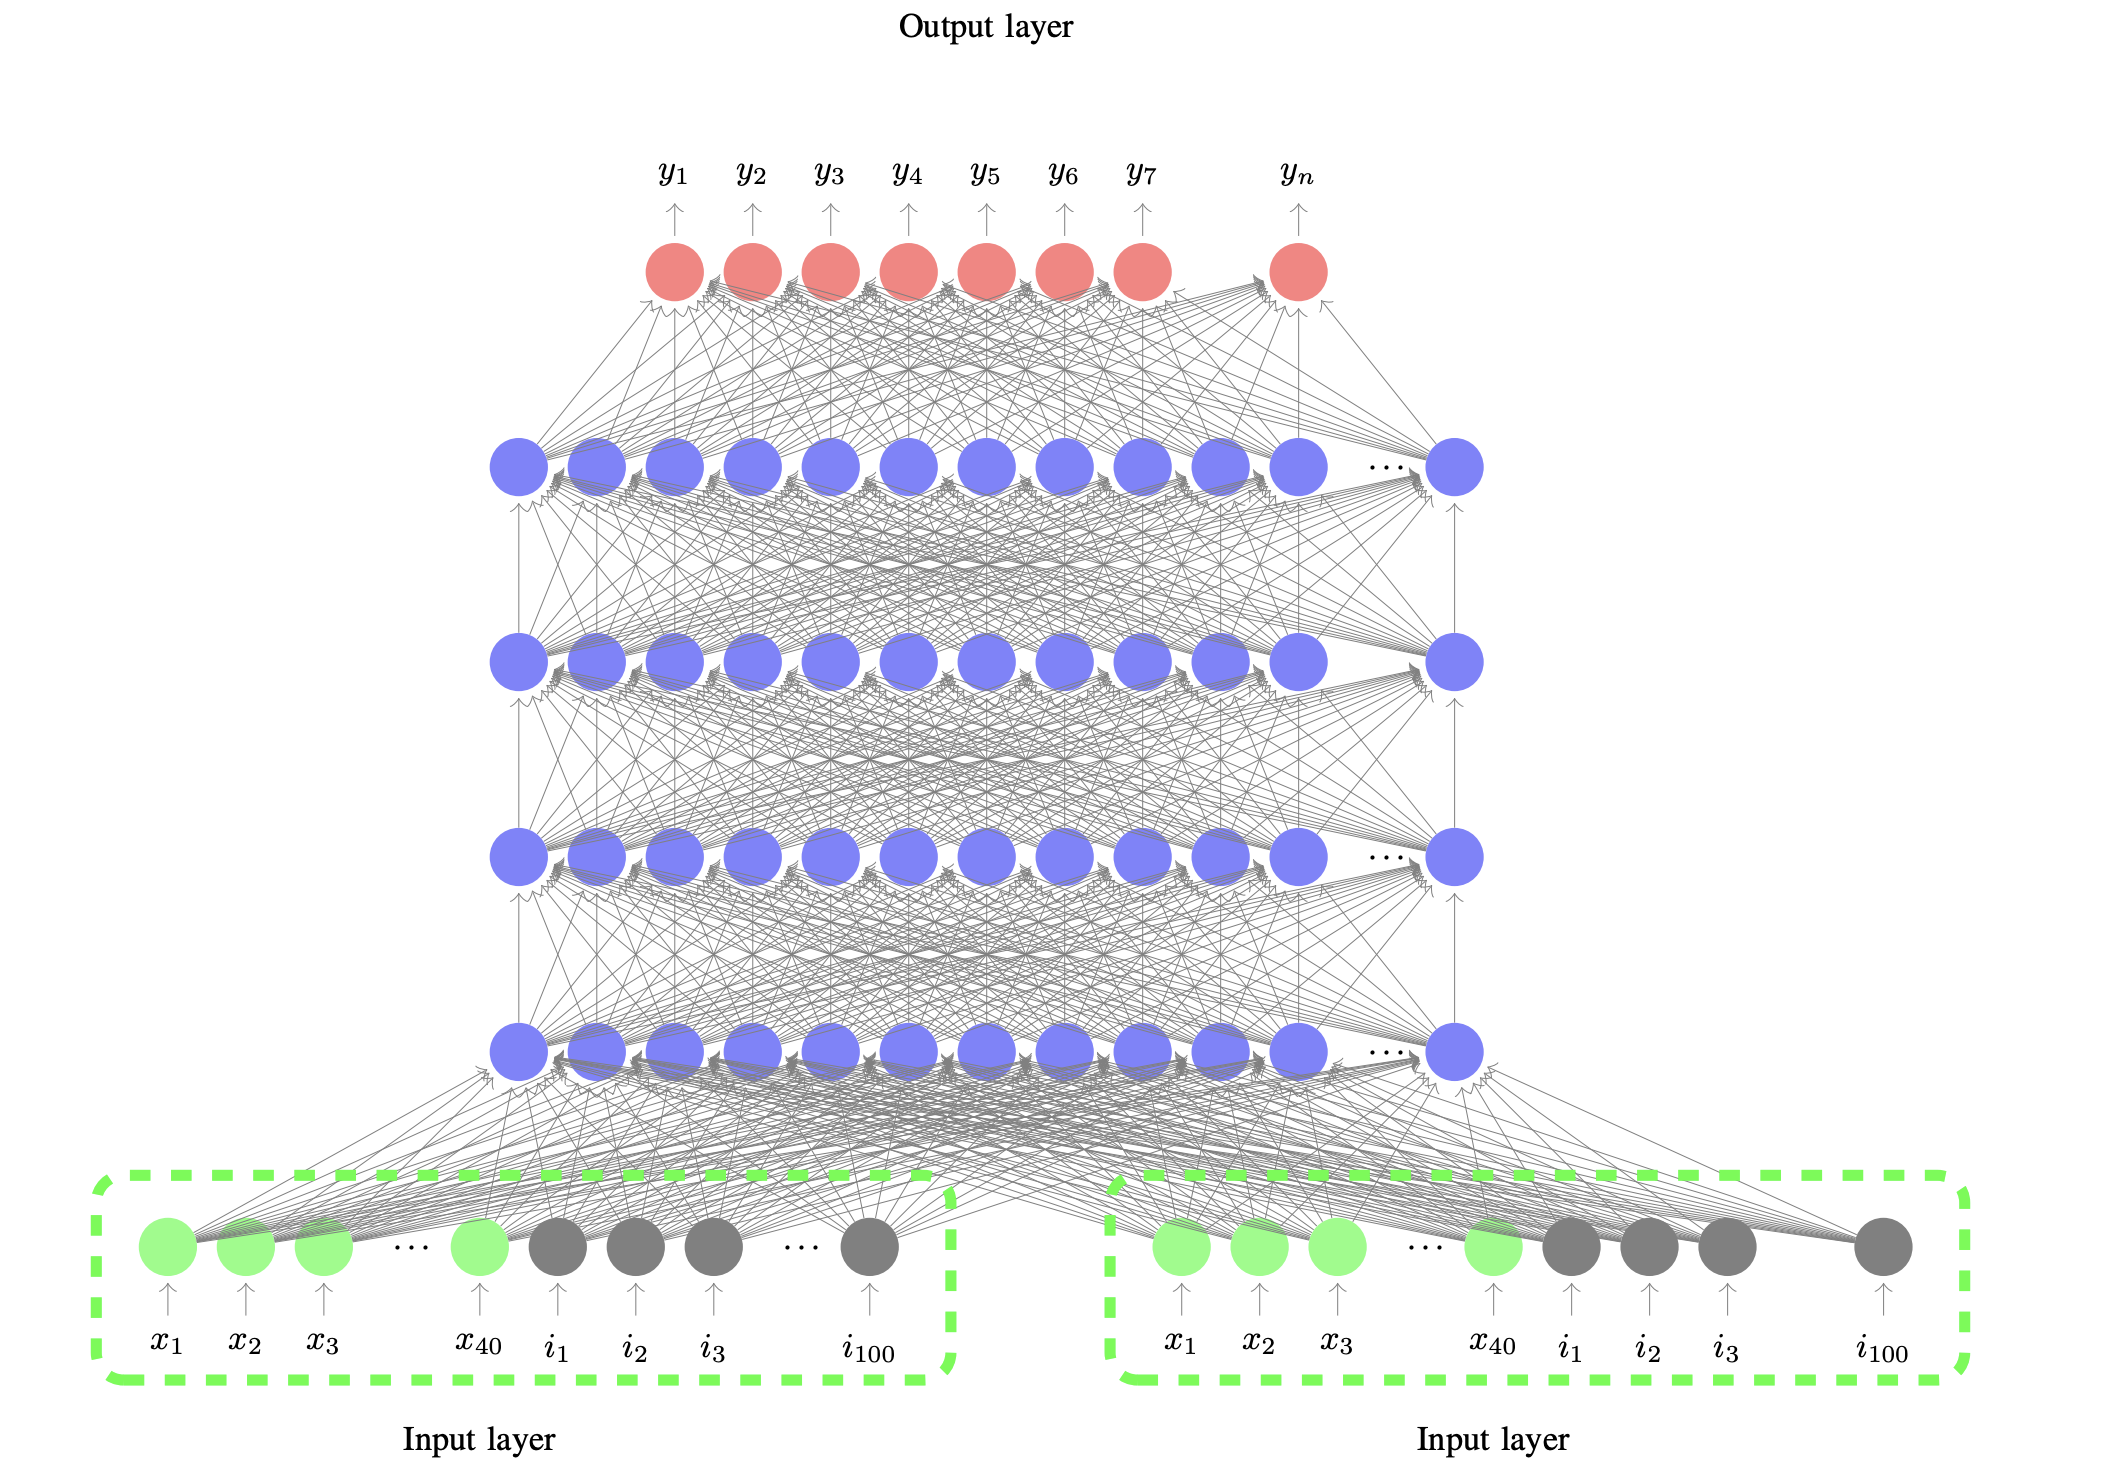
\includegraphics[width=0.48\textwidth]{imgs/tf_children.png}}
\subfigure[Pronunciation adaptation]{\label{fig:pronunciation_adapt}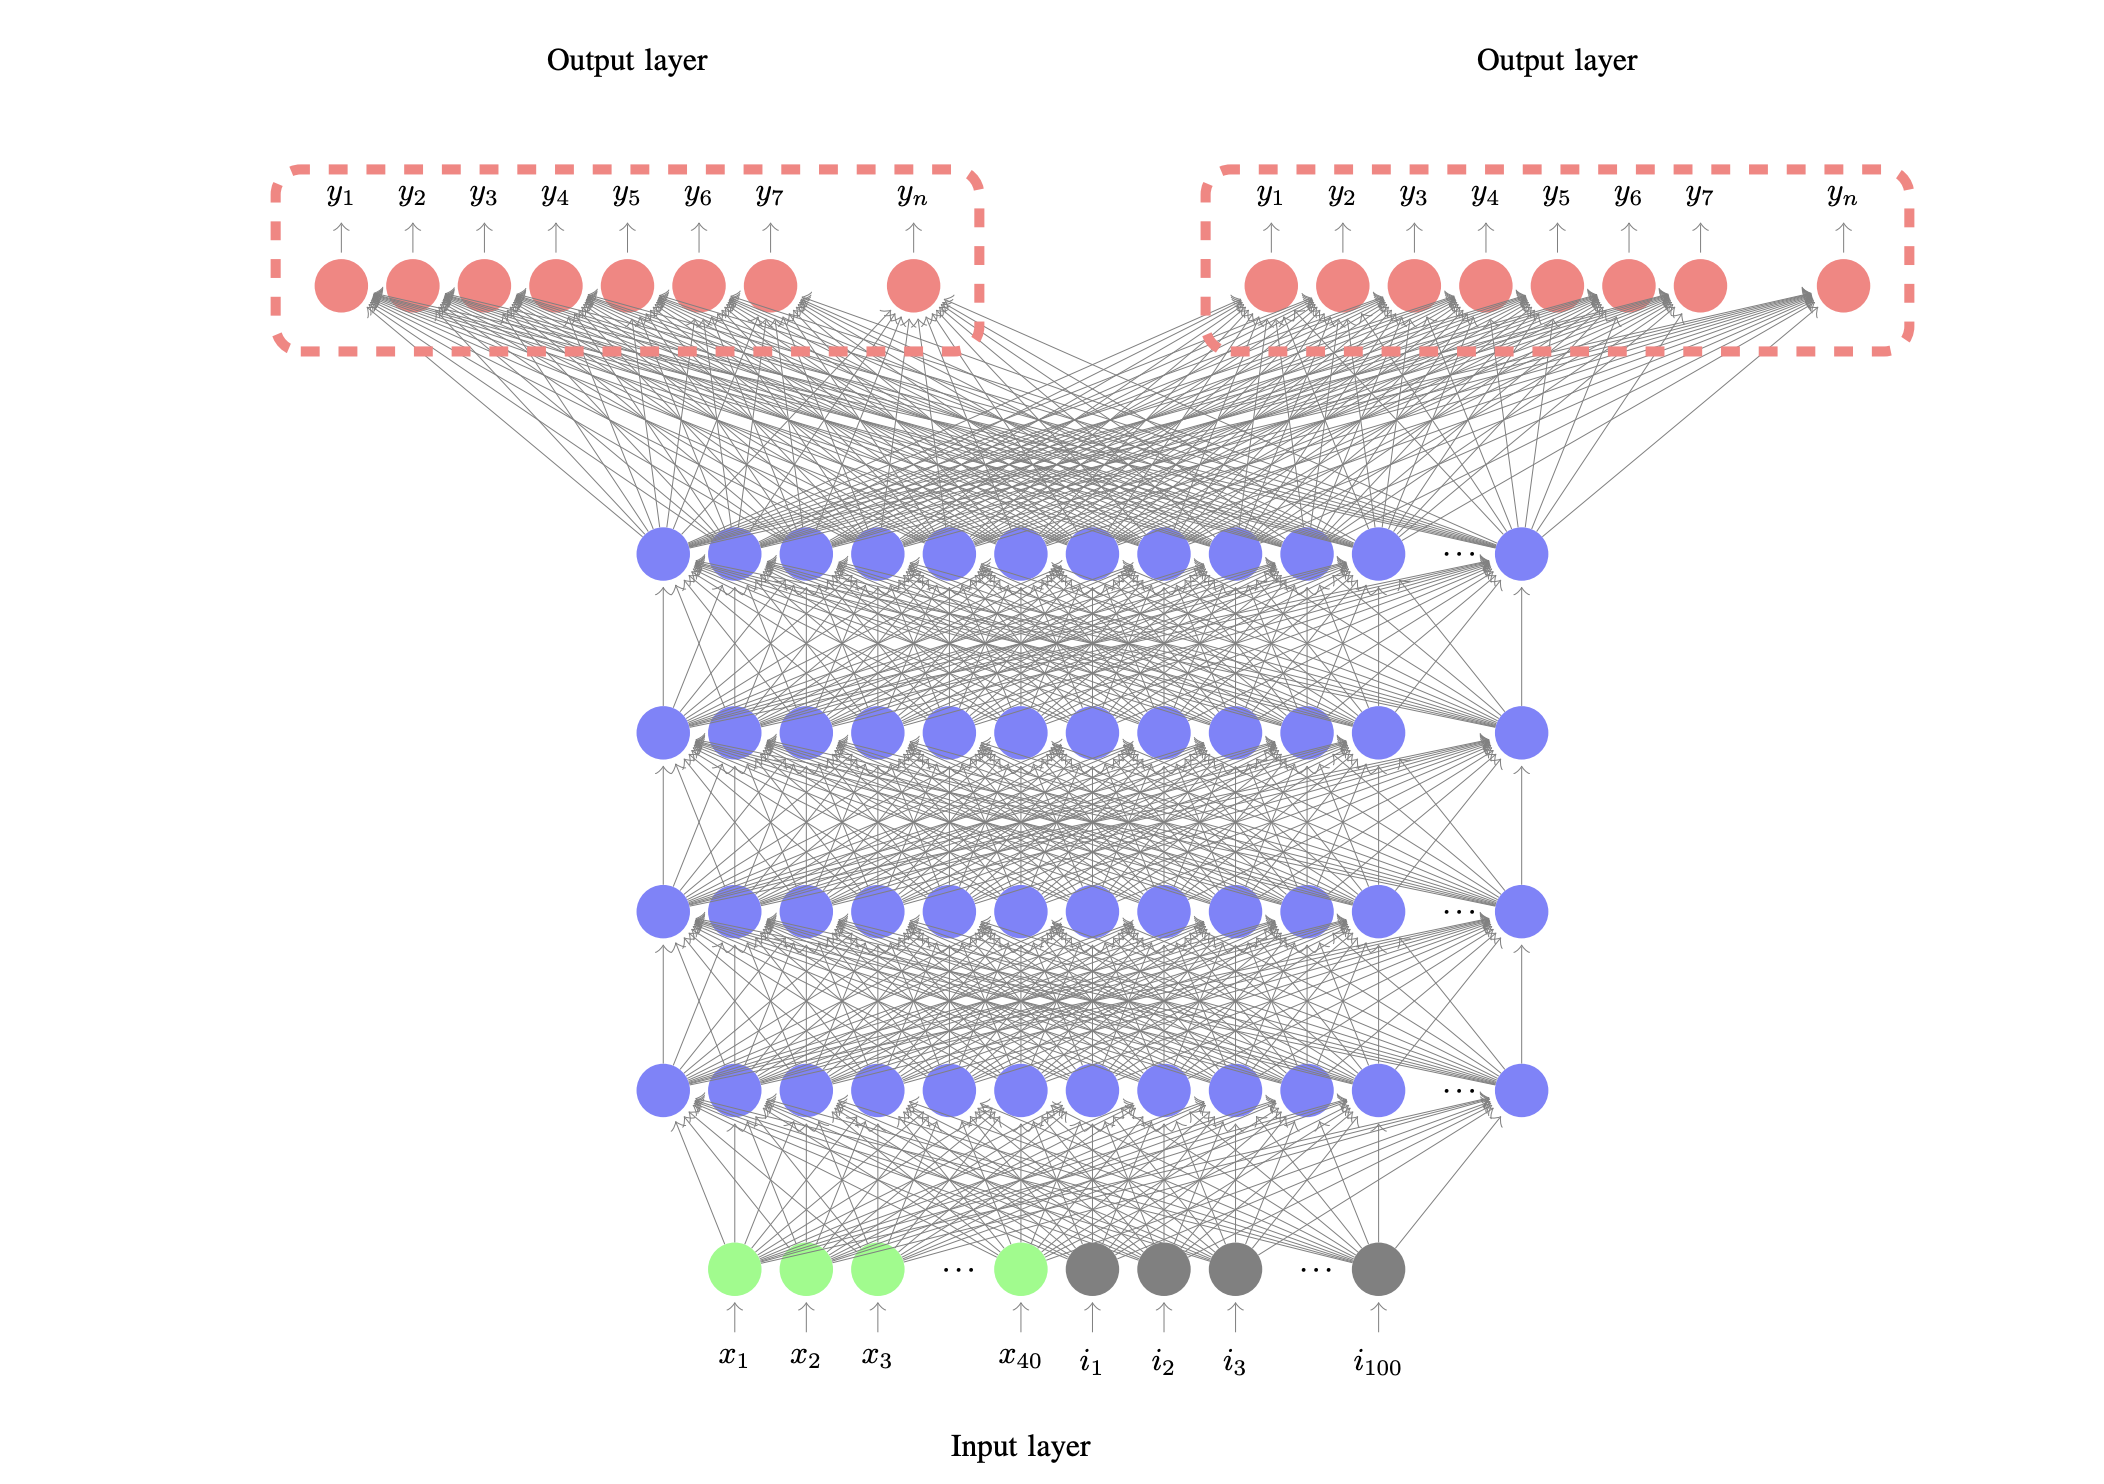
\includegraphics[width=0.48\textwidth]{imgs/pronunciation_adapt.png}}
\caption{Transfer learning approaches. Figures from \cite{TFchildren}}
\end{figure}
In recent years,\ac{TL} has emerged as a highly successful technique across various applications, particularly proving effective in low-resource tasks such as language understanding \cite{Bert}, character recognition \cite{tfcharacter}, and dysarthric speech recognition \cite{tfpathology}, among others. The achievements in these domains have spurred interest in exploring the utility of transfer learning for children's speech recognition, a domain often characterised by limited labelled data.

Given the prevalence of large corpora of adult speech, recent acoustic models trained on adult data have demonstrated high efficiency and encapsulate rich acoustic and phonetic information. Motivated by these successes, \cite{TFchildren} proposed investigating three distinct transfer learning methods to assess the contributions of acoustic adaptation, pronunciation adaptation, and their combination in the context of children's speech recognition.

Acoustic adaptation targets the lower-level layers, leveraging the established notion that these layers capture acoustic properties. The methodology involves freezing the weights of the top-level layer and applying transfer learning to the lower-level layers, as depicted in Figure \ref{fig:acoustics_adapt}. In experiments conducted by \cite{TFchildren} and \cite{TransferLF}, acoustic transfer learning from an adult model to children's speech, by retraining only the first layers, yielded substantial relative \ac{WER} improvements of 38\% and 26\%, respectively, compared to the performance of adult models. Impressively, the acoustic adaptation outperformed a randomly initialised acoustic model trained on the same children's data, achieving a 4.9\% relative \ac{WER} improvement.

Pronunciation adaptation, premised on the idea that higher-level layers capture task-specific information, focuses on adapting these layers while keeping lower-level layers frozen. As illustrated in Figure \ref{fig:pronunciation_adapt}, \cite{TFchildren} conducted experiments applying pronunciation adaptation to the last layers of the model, resulting in a significant 31\% relative \ac{WER} improvement compared to the performance of the adult model. However, when compared to a randomly initialised acoustic model trained with the same children's data, pronunciation adaptation exhibited a 5.6\% relative \ac{WER} degradation.

Finally, the combination of acoustic and pronunciation adaptation, achieved through fine-tuning the entire network, demonstrated outperforms performances compared to individual adaptations. This aligns with recent observations in end-to-end models, where transfer learning from an adult pre-trained model outperformed training from scratch using only children's data \cite{sri_end2end, gelin2021endtoend}. These findings underscore the efficacy of transfer learning strategies for optimising acoustic and pronunciation adaptation in children's \ac{ASR}. 

% Multi-task
\subsubsection{Multi-task learning}%************************************************************
\label{section:MTL}
\begin{figure}[t]
\begin{center}

\includegraphics[width=0.7\textwidth]{imgs/MTL.png}
\caption{Multilingual approach using each language as a task in a multi-task learning context.}
\label{fig:MTL}
\end{center}
\end{figure}

\ac{MTL}, like to transfer learning, draws inspiration from biological intelligence. In contrast to transfer learning, \ac{MTL} does not train solely on source and target tasks in a sequential manner, here \ac{MTL} simultaneously train on multiple tasks at the same time. The fundamental objective of \ac{MTL} is to discover shared representations among related tasks.  In general, a typical \ac{MTL} model consists of two distinct components. The first part is a sub-network shared by all tasks, while the second part consists of task-specific output sub-networks, as illustrated in Figure \ref{fig:MTL}. The shared layers facilitate the learning of a joint representation that is more robust, enhancing the model's reliability across diverse tasks.

More formally, for any task $i$ the corresponding output of the forward pass will be:
\begin{equation} \label{equation:MT}
    f(X_i;\{M_i, M_{c}\}) = f_i(f_{c}(X_i,{M_{c}}); {M_i}) 
\end{equation}
where $X_i$ is the data associated with the task $i$, $M_i$ represents the task-specific parameters of the model, and $M_{c}$ corresponds to the parameters that are shared (or common) across all tasks.

In consequence, the performances of \ac{MTL} are intricately tied to the degree of relatedness among tasks used during training. Indeed, its efficacy diminishes when confronted with outlier tasks that are unrelated to the majority of the other tasks. This sensitivity is due to the inherent challenge of learning common representations for tasks that lack substantial relatedness to one another \cite{zhang2018overview}. This task-relatedness consideration underscores the importance of thoughtful task selection when using \ac{MTL} techniques.

Moreover, \ac{MTL} has been used effectively in a variety of areas, including natural language processing \cite{multi-nlp}, computer vision \cite{mtl_computervision} and bioinformatics \cite{bioinfo}. Naturally, \ac{MTL} has been applied in the field of automatic speech recognition \cite{MTL-LFMMI} with direct application to low-resource \ac{ASR} \cite{abad2020}. Given that \ac{ASR} for children represents a resource-limited task, \ac{MTL} has been proposed as a strategy to mitigate the issue of data scarcity. Notably, studies such as \cite{TransferLF} and \cite{2019multi} successfully applied \ac{MTL} to Mandarin and English-speaking children, with a 16.96\% relative improvement in \ac{WER} for the English children.

%SSL
\subsubsection{Self-supervised Learning}
% First step is semi-supervised
A first step towards \ac{SSL} was the introduction of semi-supervised techniques, such as pseudo-labeling. Semi-supervised approaches were the dominant training strategies for using unlabeled data. In particular, the pseudo-labeling starts with the training of a ``teacher" model on a set of supervised data. Subsequently, pseudo-labels are generated for unlabeled data by leveraging the predictions of the trained teacher model. Following this, a ``student" model is trained using a combined dataset comprising both supervised and pseudo-labeled data. Importantly, the pseudo-labeling process can be iteratively repeated multiple times to enhance the quality of teacher-generated labels \cite{zavaliagkos1998utilizing,ma2006unsupervised}. It is noteworthy that, as of today, some of the most effective \ac{ASR} models, such as the Whisper model, leverage pseudo-labeling as a crucial component of its training strategy \cite{radford2023robust}. However, the performances of semi-supervised, and particularly pseudo-labelling, have been found to be highly dependent on the quality of the teacher model, prompting the need for more robust and sophisticated training strategies.

% Then comes SSL
In this context, \ac{SSL} has emerged as a paradigm designed to acquire general data representations directly from unlabeled examples, subsequently allowing transfer learning on a small amount of labelled data. This approach has proven particularly successful in the domain of natural language processing \cite{sarzynska2021detecting} and computer vision \cite{henaff2020data}.
% PASE features
One notable first attempt to bring \ac{SSL} to the speech domain was made by the introduction of the \ac{PASE} and its extension,\ac{PASE}+. These innovations demonstrated the capability to learn meaningful speech information such as speaker identities, phonemes, and emotions. The \ac{PASE} framework operates by encoding raw speech waveforms into a learned representation, which is then input to multiple regressors and discriminators. The regressors within \ac{PASE} are standard features computed from the input waveform. While the discriminators focus on positive or negative samples and are trained to effectively separate them. Both the regressors and discriminators play a crucial role in incorporating prior knowledge into the encoder, a key factor for deriving meaningful and robust representations. 

% Wav2vec2 and Hubert
Recently, \ac{SSL} systems have obtained remarkable results with the introduction of models employing \ac{BERT}-like training methodologies, such as Wav2vec2 \cite{baevski2020wav2vec} and HuBERT \cite{hsu2021hubert}. Notably, the success of these models can be attributed to the conjunction use of masking, discrete speech units, contextualised representations, and contrastive loss. The integration of masking techniques allows these models to effectively learn contextualised representations by masking certain portions of the input data and predicting them based on the remaining context. The use of discrete speech units enables the model to be more robust to variations, while the contrastive loss functions enhance the discriminative power of these models by encouraging the model to differentiate between positive and negative samples.

% SSL for children
Motivated by the capabilities of \ac{SSL} methods in overcoming challenges in low-resource \ac{ASR} tasks, such as low-resource languages \cite{riviere2020unsupervised}, noisy speech \cite{wang2022wav2vec}, and accented speech \cite{li2021accent}, the integration of \ac{SSL} for children's \ac{ASR} marked its debut in 2021, with a first place in a non-native children's speech recognition challenge \cite{xu2021tal}. Subsequent to this notable success, the application of \ac{SSL} for children's \ac{ASR} has gained increased attention, especially with the use of models like Wav2vec2 \cite{jain2023wav2vec2,jain2023adaptation,fan2022draft}. A concise analysis of various \ac{SSL} approaches as frozen feature extractors for children's \ac{ASR} has been conducted within the context of this thesis, and the findings are presented in Annex \ref{chapter:appendixB}.
   
\section{Children Corpora}
\label{section:children_corpora}
As described in Chapter \ref{section:data_scarcity}, notwithstanding recent efforts to assemble dedicated databases for children's speech, the quantity of available data remains lower compared to adults. Collecting speech data from children is challenging in many ways, from factors such as limited attention spans, frequent mispronunciations, ungrammatical expressions, and the use of non-standard vocabulary. These difficulties involved in capturing high-quality child speech data contribute to the scarcity of publicly accessible child speech corpora. Additionally, the relatively modest sizes of these datasets present obstacles to research efforts and impede progress in developing reliable \ac{ASR} systems for children.


\begin{table}
%\centering
\small
\begin{tabular}{l|c|c|c|c|c|c} 
\hline
\multicolumn{1}{c|}{\textbf{Corpus}} & \multicolumn{1}{c|}{\textbf{Languages}} & \multicolumn{1}{c|}{\textbf{\# Spkrs}} & \multicolumn{1}{c|}{\textbf{\# Utt}} & \multicolumn{1}{c|}{\textbf{Dur.}} & \multicolumn{1}{c|}{\textbf{Age Range}} & \multicolumn{1}{c}{\textbf{Date}} \\ 
\hline
Providence Corpus \cite{providence} & English & 6 &  & 363h & 1-3 & 2006 \\ 
\hline
Lyon Corpus \cite{LyonSC} & French & 4 &  & 185h & 1-3 & 2007 \\ 
\hline
CASS\_CHILD \cite{cass_child} & Mandarin & 23 &  & 631h & 1-4 & 2012 \\ 
\hline
Demuth Sesotho Corpus \cite{demuth1992acquisition} & Sesotho & 4 & 13250 & 98h & 2-4 & 1992 \\ 
\hline
NITK Kids’ Speech Corpus \cite{nitk} & Kannada & 160 &  & 10h & 2-6 & 2019 \\ 
\hline
CHIEDE \cite{chiede} & Spanish & 59 & 15,444 & 8h & 3-6 & 2008 \\ 
\hline
CUChild \cite{cuchild} & Cantonese & 1,986 &  &  & 3-6 & 2020 \\ 
\hline
EmoChildRu \cite{emochildru} & Russian & 100 & 20,000 & 30h & 3-7 & 2015 \\ 
\hline
CNG Portuguese children\cite{hamalainen2013cng} & Portuguese & 510 &  & 21h & 3-10 & 2013 \\ 
\hline
AusKidTalk$^1$ \cite{ahmed2021auskidtalk} & English & 750 &  & 600h & 3-12 & 2021 \\ 
\hline
UCLA JIBO kids \cite{yeung2019robotic} & English & 130 &  &  & 4-7 & 2019 \\ 
\hline
\textbf{PF-STAR-SWEDISH} \cite{pfstar}
& Swedish & 198 & 8,909 & 6h & 4-8 & 2005 \\ 
\hline
SLT 2021 \cite{yu2021slt} & Mandarin & 981 &  & 58h & 4-11 & 2021 \\ 
\hline
PF-STAR Children British \cite{pfstar,russell2006pf,pf-star-british} & English & 158 &  & 14.5h & 4-14 & 2006 \\ 
\hline
AD-child. RU \cite{ad-child_ru} & Russian & 278 &  &  & 4-16 & 2019 \\ 
\hline
TBALL \cite{tball} & English & 256 & 5,000 & 40h & 5-8 & 2005 \\ 
\hline
SPECO \cite{speco} & Hungarian & 72 &  & 12h & 5-11 & 1999 \\ 
\hline
UltraSuite\cite{eshky2019ultrasuite} & English & 86 & 14,456 & 37h & 5-14 & 2019 \\ 
\hline
CID read speech corpus \cite{lee1999acoustics} & English & 436 &  &  & 5-18 & 1996 \\ 
\hline
Persian Kids Speech Corpus \cite{khanzadi2022persian} & Persian & 286 & 162,395 & 33h & 6-9 & 2022 \\ 
\hline
\textbf{Letsread$^2$} \cite{letsread} & Portuguese & 284 & 4,629 & 14h & 6-10 & 2016 \\ 
\hline
\textbf{CMU kids Corpus} \cite{cmu} & English & 76 & 5,180 &  & 6-11 & 1997 \\ 
\hline
CFSC \cite{CFSC} & Filipino & 57 &  & 8h & 6-11 & 2012 \\ 
\hline
IESC-Child \cite{PEREZESPINOSA202055} & Spanish & 174 & 19,793 & 34h & 6-11 & 2020 \\ 
\hline

CU Children's read and prompted \cite{hagen2003children}& English & 663 & 66300 &  & K-G5 & 2001 \\ 
\hline
\textbf{Chorec$^2$} \cite{chorec} & Dutch & 400 & 3,065 & 25h & 6-12 & 2008 \\ 
\hline
ChildIt2 \cite{childit2} & Italian & 96 &  4,875 & 9h & 6-14 & 2016 \\ 
\hline
TIDIGITS \cite{leonard1993tidigits} & English & 101 &  &  & 6-15 & 1993 \\ 
\hline
CSLU Kids' Speech Corpus \cite{cslu} & English & 1,100 & 1,017 &  & K-G10 & 2007 \\ 
\hline
SingaKids-Mandarin \cite{singakids} & Mandarin & 255 & 79,843 & 125h & 7-12 & 2016 \\ 
\hline
ChildIt corpus \cite{gerosa2006acoustic} & Italian & 171 &  &  & 7-13 & 2007 \\ 
\hline
VoiceClass Database \cite{burkhardt2010database} & German & 170 &  &  & 7-14 & 2010 \\ 
\hline
Deutsche Telekom telephone \cite{burkhardt2010database} & German & 106 &  &  & 7-14 & 2010 \\ 
\hline
Jasmin \cite{JASMIN} & Dutch &  &  & 63h & 7-16 & 2008 \\ 
\hline
Tgr-child corpus \cite{gerosa2006acoustic} & Italian & 30 &  &  & 8-12 & 2007 \\ 
\hline
SponIt corpus \cite{gerosa2006acoustic} & Italian & 21 &  &  & 8-12 & 2007 \\ 
\hline
Swedish NICE Corpus \cite{bell2005swedish} & Swedish & 75 & 5,580 &  & 8-15 & 2005 \\
\hline
CHIMP spontaneous speech \cite{language_children2} & English & 160 &  &  & 8-14 & 2002 \\ 
\hline
SpeeCon corpus  \cite{SPEECONS} & 20 Languages &  &  &  & 8-15 & 2002 \\ 
\hline
Rafael.0 telephone corpus \cite{linguistic-children} & Danish & 306 &  &  & 8-18 & 1996 \\ 
\hline
\textbf{Boulder Learning - MyST} \cite{MyST} & English & 1,371 & 228,874 & 384h & G3-G5 & 2019 \\ 
\hline
CU Story Corpus \cite{hagen2003children} & English & 106 & 5,000 & 40h & G3-G5 & 2003 \\ 
\hline
\textbf{ETLT$^2$} \cite{etlt} & L2 German &  & 1,674 & 6h & 9-16 & 2020 \\ 
\hline
Lesetest corpus \cite{grissemann2000zurcher} & German & 62 &  &  & 10-12 & 2000 \\ 
\hline
FAU Aibo Emotion Corpus \cite{steidl2009automatic} & German & 51 & 13,642 & 9h & 10-13 & 2002 \\ 
\hline
PIXIE corpus \cite{bell2003child} & Swedish & 2,885 &  &  &  & 2003 \\ 
\hline
Takemaru-kun corpus \cite{takemaru} & Japanese & 17,392 &  &  & & 2007 \\ 
\hline
CALL-SLT \cite{callslt} & German &  & 5,000 &  &  & 2014 \\ 
\hline
\multicolumn{7}{l}{$^1$ To this day, data collection for this dataset is not complete.} \\
\multicolumn{7}{l}{$^2$ Information displayed here correspond to a subset of the original data used in this proposal.}  \\
\end{tabular}
\caption{Non-exhaustive comparison of children's speech corpora. This table has been sorted by age range. Blanks indicate unavailable information. Entries highlighted in bold correspond to the corpora used in the experiments presented in this thesis. K: Kindergarden. G: Grade}
\label{table:children_corpora}
\end{table}

Table \ref{table:children_corpora} provides a compilation of existing corpora of children's speech. Notably, approximately one-third of the available corpora are in English. Likewise, a comparable proportion is specifically oriented towards children under the age of 4, where the speech dataset comprises child-adult interactions (usually with the parents). It is crucial to acknowledge the inherent trade-offs in these different corpora, involving considerations of speaker diversity, total duration, and the number of utterances.

Subsequently, the remainder of this section will provide a more detailed description of the children's speech corpora employed in this thesis.


\subsection{LETSREAD}
LetsRead database \cite{letsread} is a read-aloud speech database of European Portuguese from children aged 6 to 10,  from 1st to 4th grade. This corpus is composed of a total of 284 children, 147 girls and 137 boys, whose mother tongue is European Portuguese. Children from private and public Portuguese schools were asked to carry out two tasks: reading sentences and a list of pseudo-words. The difficulty of the tasks varies depending on the school year of the child. 
For this proposal, we excluded all utterances from the pseudo-word reading task because we do not include pseudo-words in the language model and lexicon in our experiments. 
\subsection{PFSTAR\_SWEDISH}
The PFStar children's speech corpus \cite{pfstar} was collected as part of the EU FP5 PFSTAR project. It contains more than 60 hours of speech. This corpus is divided into two parts: native-language speech and non-native language part.
The native-language speech part contains recordings of British English, German and Swedish children, from 4 to 14 years old. The non-native language part consists of speech by Italian, German and Swedish children speaking English. In this work, we only used the native language Swedish part, consisting of speech by 198 native Swedish children, between 4 and 8 years old recorded in the Stockholm area, imitating an adult who read the text from a screen.
\subsection{ETLTDE}
\ac{ETLT} corpus \cite{etlt} has been collected in northern Italy for assessing English and German proficiency of Italian children between 9 and 16 years old, by asking them to answer questions. The data collection was carried out in schools. On average the signal quality is good, but some background noise is often present (doors, steps, keyboard typing, background voices, street noises if the windows are open, etc). In addition, many answers are whispered and difficult to understand.
For this thesis, we only used the German-transcribed subset, named ETLTDE, a subset containing around 6 hours of speech divided into training and test partitions.
\subsection{CMU\_KIDS}
The \ac{CMU} kids corpus \cite{cmu} contains English sentences read aloud by children, 24 males and 52 females, from 6 to 11 years old. In total, 5,180 utterances were recorded with one sentence per utterance. This database was created to train the SPHINX II \cite{sphinx2} automatic speech recognition system within the LISTEN project at \ac{CMU}.
\subsection{CHOREC}
\label{subsection:chorec}
The Chorec corpus \cite{chorec} consists of 400 Dutch-speaking elementary school children, between 6 and 12 years old, reading words, pseudo-words and stories. The difficulty of the reading task was adapted to children with 9 different levels. Recordings were made in schools, leading to some environmental noises (school bells, children entering the playground etc.). For this thesis, similarly to the LETSREAD dataset, we discarded pseudo-word utterances.

\subsection{MyST}
\ac{MyST} Children Speech Corpus \cite{MyST} is currently one of the largest publicly available corpora of English children's speech, with around 400 hours. This is about 10 times more than all other English children's speech corpora combined. It consists of conversations between children and a virtual tutor in 8 scientific domains. Speech was collected from 1,372  students in the third, fourth and fifth grades. Partitioning of the corpus is already available, ensuring a reasonable representation of each scientific domain and that each student is present in only one partition. However, only 45\% of the utterances were transcribed at the word level. Furthermore, for the purposes of all our experiments in the thesis, we decided to remove all utterances shorter than one second and longer than 20 seconds and shorter than one second. Typically, utterances shorter than one second were found to predominantly contain silence alone, while those longer than 20 seconds were constrained by our GPU limitations. After this filtering, 81971 utterances from 736 speakers for a total of 151 hours remain.


\section{Summary}
In this chapter, we provided an overview of children's \ac{ASR}, its inherent challenges, and the ongoing responses from the research community. The complexity of \ac{ASR} in children arises primarily from the developmental nuances of the vocal apparatus, resulting in an acoustic mismatch with adult speech, although this mismatch gradually diminishes until around the age of 15. Despite sustained efforts, \ac{ASR} for children remains an active and challenging area of research.

Our examination in this chapter highlights that knowledge transfer approaches, such as transfer learning and multi-task learning, appear to be promising avenues for improving children's \ac{ASR}. Additionally, the exploration of synthetic speech generation, using \ac{TTS} systems, has captured our attention as a potential strategy for improvement. These methodologies will be applied and explored in-depth in the subsequent chapters of this thesis.

Moreover, we have presented a comprehensive comparison of children's speech corpora, which, to the best of our knowledge, stands as the most exhaustive compilation available. This analysis provides valuable insights into the landscape of available datasets for children's speech.

% If Printing on DOUBLE SIDED pages, the second page should be white.
% Otherwise, comment the following command:
\cleardoublepage{}
%
%Chapter 3
%% #############################################################################
% This is Chapter 3
% !TEX root = ../main.tex
% #############################################################################
\fancychapter{Hybrid models for children automatic speech recognition}
\label{chap:Chapter3}
\cleardoublepage
\section{Introduction}
% HMM-DNN played a signifant role in ASR (quick history recap)
In the history of ASR, HMM-based models emerged as a popular choice for acoustic modeling since the 1980s. The application of HMMs offered a structured framework to effectively model the temporal dependencies inherent in speech signals.The initial paradigm involved combining HMMs with GMMs to represent the probability distributions of acoustic features. This traditional HMM-GMM architecture, while effective to a certain extent, faced limitations in capturing the intricacies of complex, non-linear relationships present in speech data. Therefore, a pivotal turning point occurred with the integration of DNN, evolving towards hybrid HMM-DNN models. This paradigm shift lead to substantial improvements in ASR performances. Inded, DNNs brought enhanced modeling capabilities, allowing the system to discern more nuanced acoustic patterns and adapt better to diverse linguistic contexts. The hybrid HMM-DNN approach has become key architecture in modern ASR systems, demonstrating remarkable success in handling large vocabulary tasks and challenging acoustic conditions \cite{!!}. 

% Why HMM-DNN for children
In Chapter \ref{chap:Chapter2}, we saw how a HMM-GMM or HMM-DNN ASR system can directly integrate relevant knowledge into the ASR pipeline. This knowledge is transmited to the pipeline using the language model, acoustic model, and vocabulary. Having hand-crafted knowledge directly in the ASR system allows to reduce the amount of speech data required to generate appropriate results. Such characteristics was found beneficial for children ASR where the amount of data is limited. According to the literature, a common family of methodologies  found to be benefits in improving ASR results are the inductive bias approaches such as transfer learning and multi-task learning \cite{TransferLF}. For years, HMM-based configurations have been a privileged setting for the children's ASR community. As a matter of fact, between 2009 and 2020, 80\% of published research on children's speech recognition was based on hybrid systems, with 45\% using HMM-GMM and 35\% HMM-DNN. However, one notable observation was that during the same period, 63\% of published work was conducted for English \cite{big_review_childASR}. As a result, it is uncertain how children's speech from other languages relates to the various approaches used in English, particularly transfer and multi-task learning.

% What we planned to do here
In this chapter, we will first present the factorised time delay neural network in HMM-DNN ASR system. Then, we will delve into applying knowledge transfer strategies applied across various scenarios, encompassing both non-English and English datasets. Applying it to non-English dataset will allow us to understand if inductive bais approaches are still working in the context of non-English children speech. To this end, we present an examination of transfer and multi-task learning methodologies, leveraging adult speech as an inductive bias, a prevalent approach in the existing literature. 

Finally, as our contribution, we introduce a novel approach termed "multilingual transfer learning". This strategy integrates both transfer and multi-task learning techniques, where we address the challenge posed by the scarcity of data for both adult and children's in low-resource languages by using the combination of transfer and multi-task learning methodologies but restrict our focus solely to low-resourced  children's speech datasets.
%aiming to obtain a better ASR model for children.
%This chapter will investigate these strategies in a variety of scenarios employing non-English data and English data. First, we present transfer and multi-task learning using adult speech as an inductive bias, as is common in the literature. Second, because there is a lack of data for both adult and children's low-resource languages, we investigate the same methodologies using only children's speech. Finally, we present our approach, multilingual transfer learning, which combines transfer and multi-task learning to produce a more robust model for speech recognition in low-resource children setting.

\section{Factorised Time Delay Neural Network for children ASR}
% Explain that we won't reexplain HMM-DNN models but only the DNN we use here 
% Motivation
An alternative avenue for enhancing ASR performance in scenarios characterised by limited child speech data involves the exploration of more data-efficient neural network architectures. One notable example is the Factorised Time-Delay Neural Network (TDNN-F).The TDNN-F architecture represents a variation of traditional TDNNs designed to be more computationally efficient and capable of learning robust representations from limited data. 
% What is TDNN-F

% How its used
%By employing TDNN-F in ASR for child speech, researchers aim to strike a balance between model complexity and data availability. The architecture's ability to generalize well with fewer parameters makes it well-suited for scenarios where obtaining large amounts of labeled child speech data is impractical. This approach aligns with the broader trend in developing neural network architectures that are both computationally efficient and effective, especially when faced with limited training samples.

%In summary, leveraging more data-efficient network architectures like TDNN-F represents a promising approach to address the challenges of limited child speech data in ASR. This strategy aims to enhance the model's ability to learn meaningful representations from a modest dataset, ultimately contributing to more accurate and robust speech recognition systems for children.

\section{Multi-task and Transfer learning using adult and children data}
\label{section:HMMDNNADULT2CHILD}
\subsection{Methodology}

% Motivation
Motivated by the success of knowledge transfer approaches for ASR children using adult data in the research \cite{TFchildren,TransferLF,2019multi}, we intend to validate these findings using a low-resource language. Indeed, using adult data for pre-training makes sense since adult speech is more stable and less prone to variation. Using adult speech to train a speech recognition algorithm makes it simpler to extract and recognize intrinsic and meaningful speech patterns.
% Quick recap on TL and MLT

For this proposal, we assess children's speech recognition performances in four distinct configurations:
\begin{enumerate}
    \item \textbf{Adult model}: Using a model trained from scratch with only adult data.
    \item \textbf{Children model}: Using a model trained from scratch with only children data.
    \item \textbf{Multi-task model}: Using a model trained jointly on adult and children data in parallel using multi-task learning.
    \item \textbf{Transfer learning}: Using a model that has been fine-tuned on children data from the adult model of configuration 1.
    %\item \textbf{Transfer learning with well-resource corpus}:  Using a model that has been finetuned on children data from the adult model trained on large amount of adult English data.
\end{enumerate}

\subsection{Corpus}
\label{sec:corpus}
As stated in the introduction, we aim to evaluate the performance of children's speech in a low-resource language. To this end, we decided to use European Portuguese corpora. European Portuguese can be considered a low-resource language since most adult speech corpora do not exceed 100 hours \cite{tribus}.
In this experiment, we used LetsRead, a child corpus, described in section \ref{section:children_corpora} and BD-PUBLICO as adult corpus. %However, given the relatively small size of BD-PUBLICO, we chose to expand our experiments with a large English corpus, Librispeech-960. 
The statistics of all these two corpora are provided in the following table \ref{tab:statistics_exp1}. The rest of this section provides further information about the BD-PUBLICO corpus.%these two adult corpora.

% Stat corpus 
\begin{table}[h]
\begin{center}
\begin{tabular}{lcc}
\hline
Corpus name      & Train & Test  \\ \hline
\multicolumn{1}{l}{BD-PUBLICO}             & 8085 utt  & 412 utt  \\ 
\multicolumn{1}{c}{\textit{Adult}}              & 21h48 & 01h10 \\\hline
\multicolumn{1}{l}{LETSREAD}     & 3590 utt & 1039 utt \\ 
\multicolumn{1}{c}{\textit{Children}}     & 12h00 & 02h30 \\  \hline
%\multicolumn{1}{l}{Librispeech}                     & 281241 utt &   \\ 
%\multicolumn{1}{l}{}      &                &  960h &  \\ \hline
\end{tabular}
\caption{Number of utterances and duration of the different corpora for multi-task and transfer learning experiments using adult and children data}
\label{tab:statistics_exp1}
\end{center}
\end{table}

\subsubsection*{BD-PUBLICO}
The BD-PUBLICO database (Base de Dados em Português eUropeu, vocaBulário Largo, Independente do orador e fala COntínua) \cite{bdpublico} consists of reading sentences extracted from Portuguese newspaper PÚBLICO. The sentences that are read correspond to a total of 6 months of news (equivalent to 10M words and 156k different forms). It is composed of 120 speakers, and graduate and undergraduate students from Instituto Superior Técnico (Lisbon). This corpus is considered an adult dataset since all students are between 19 and 28 years old. All recordings were performed in good noise condition, in a soundproof room at INESC-ID (Lisbon), at a sampling frequency of 16kHz and using a high-quality microphone. In addition, a pronunciation lexicon with citation phonemic transcriptions for each word was produced. Finally, manually corrections were applied to the automatically generated transcriptions. 

We divided the BD-PUBLICO corpus into three unique sets with balanced gender partitioning: 1) A training set of 80 sentences by 100 speakers. 2) A development set of 40 sentences performed by a total of 10 speakers. Finally, a test set of 40 sentences by 10 speakers.

%\subsubsection*{Librispeech}
%Librispeech corpus is one of the biggest publicly available speech dataset \cite{librispeech}. It is a collection of 982 hours recorded at 16kHz from 2484 adult speakers derived from audiobooks. Librispeech corpus is designed to ensure a gender balance and no speaker overlap between train, development and test sets.


\subsection{Experimental setup}
\label{section:exp_setup}

All experiments were carried out using the Kaldi open-source toolkit \cite{kaldi}. First, for each corpus, an independent HMM-GMM acoustic model was trained to produce the necessary alignment for the HMM-DNN model. Then, HMM-DNN acoustic models were trained using  40-dim filter-banks (fbanks) in addition to a 40-dim Spectral Subband Centroid (SSC) features \cite{ssc}. These features are known to have similar properties to formant frequencies. Thus, we expect them to help vowel recognition and lead to better recognition of children's speech. 
The resulting 80-dim input features are then augmented by a 100-dim i-vector. Concatenating speaker embeddings to the input features helps to improve model speaker robustness \cite{ivector}. For our experiments, we use an i-vector extractor trained on a set of pooled children data from different languages.

Data augmentation was applied to all training corpora by perturbing the speaking rate of each training utterance by 0.9 and 1.1 factors; as well as volume perturbation. This helps the network to be more robust to rate and volume variability on the test sets. To further improve the robustness of the model, Specaugment \cite{specaugment}  was applied on top of the fbanks and SSC features by randomly masking time and frequency bands.

For all experiments, we kept the same HMM-DNN acoustic model architecture using lattice-free maximum mutual information (LF-MMI) objective with a learning rate of 2.0E-4. The acoustic model architecture is divided into two parts: i) six convolutional neural network layers and seven TDNN-F layers of dimension 1024  and followed by ii) two TDNN layers of dimension 450 and a fully-connected layer.

For the transfer learning experiments, only the first part of the network will be fine-tuned, while the second part will be dropped and replaced by randomly initialized ones. Similarly, for the multi-task learning experiment, the first part will be shared between the adult and the child, while the second part will be independent.



\subsection{Results}
\begin{table}[h]
\centering
\begin{tabular}{c|ccc}
\hline
 Method & Adult WER $\downarrow$   & Children WER  $\downarrow$   \\ \hline
\multicolumn{1}{c|}{Adult model} & 3.82\%   &  102.83\%\\ 
\multicolumn{1}{c|}{Children model} & 45.56\%  & 26.88\% \\ 
\multicolumn{1}{c|}{Multi-task model}  &   4.59\% &  27.65\% \\ 
\multicolumn{1}{c|}{Transfer learning} &  -  & 25.36\% \\ \hline
%\multicolumn{1}{c|}{Transfer learning from Librispeech} & -  & 25.18\% \\ \hline


\end{tabular}

\caption{WER results using adult data for knowledge transfer methods}
\label{tab:res_exp1}
\end{table}

% Adult model
The WER scores for all settings are presented in table \ref{tab:res_exp1}. In the first row, we notice that employing a model trained on adult data yields a WER of 102.83\% on the children's test set. This model achieves 3.82\% for BD-PUBLICO. This degradation in the children's compared to adults' scores demonstrates the presence of considerable variability in children's speech, which has a detrimental impact on the ASR scores. It supports the idea that an acoustic model designed exclusively for children is necessary because child speech is currently unusable with adult systems.

% Children model
Training the acoustic model directly on the children's data, on the other hand, considerably improved the word error rate on the children's data to 26.88\%. Since the model observes acoustic variability during training, it becomes more robust to it. While the model improved for children, it deteriorated adult speech recognition performance to 45.56 \% WER. This confirms the acoustic mismatch between adult and children speech once more. We compare transfer and multi-task learning approaches using these two experiments as a baseline.

% Multi-task
When the model was trained jointly utilising adult and children data in the scenario of multi-task learning, the recognition score of the adults and children decreased marginally when compared to the adult and child model baselines. Unlike in the adult and child models, where the mismatch significantly reduced the children's score in the adult model and the adult's score in the child model, both recognition scores in this multi-task learning scenario are comparable to their respective "trained from scratch" baselines. These results were achieved by including corpus-specific layers into the acoustic model architecture. 
Indeed, the model's shared component will learn the key characteristics of Portuguese speech, while the corpus-specific part will focus on how to apply them to adults and children, respectively.

% TL BD-Publico
In the fourth line, Training over children data with a pre-trained Portuguese adult model as initialization enhanced the result to 25.36\% WER. When compared to weights random initialization, it is shown that the weights of the adult model are a beneficial starting configuration and allow the transfer learning model to learn relevant patterns for children. It avoids the need for the model to learn these patterns from scratch, using data from a highly variable source. As a result, transfer learning may be considered a viable strategy for improving the ASR performance for children's speech. This finding is consistent with the literature on hybrid models\cite{TransferLF,TFchildren}. 

% TL Librispeech
%Finally, employing transfer learning from well-resourced but out-of-domain speech data, here Librispeech, improves recognition scores for Portuguese children, with a 25.18\% WER. When compared to weights random initialization, it shown that the weights of the English model are a beneficial starting configuration and allow the transfer learning model to attain learn relevant patterns for children.In the literature, similar behavior has been reported \cite{kunze2017transfer}.

\subsection{Summary and discussion}
% Conlusion
In this study, we conducted a knowledge transfer technique analysis to improve the results of ASR systems for children. We corroborate the acoustic mismatch between adult and child speech and the importance of the model encountering child data and its variability. Our investigations revealed that the transfer learning approach is a promising way to improve low-resource children's speech recognition scores. Furthermore, multi-task learning was found to be helpful in the setting of mixed adult-child ASR acoustic modelling.
% Open question for next section
However, in this study, we focus on the transfer from adults to children. It is not clear how such a system can work using only children's data.



\section{Multi-task and transfer learning using multilingual children data}
\subsection{Motivation}
% Explain motivation
In this section, we study whether the performance of children's ASR for low-resourced languages may be improved by combining children's resources from different languages. In many cases, there is limited or no data for both adults and children. Therefore, we propose using several small-sized corpora of children from various languages to overcome the substantial acoustic variability and data scarcity issues. The current study extends standard multilingual training and transfer learning for hybrid HMM-DNN ASR by combining them in a meaningful way to use knowledge from heterogeneous data. First, a multilingual model trained with a multi-task learning objective tries to optimise network parameters to the specific characteristics of children's speech in multiple languages/tasks simultaneously. Subsequently, this multilingual model is used to improve ASR for a target language --potentially different from those used in the multilingual training stage-- by using transfer learning. We address the following research question: Does this two-step training strategy outperform conventional single language/task training for 's speech, as well as multilingual and transfer learning alone?

\subsection{Proposed approach}
\label{section:method}
We propose to combine transfer learning (TL) and multi-task learning (MTL) together for improved acoustic modelling of hybrid HMM-DNN ASR.
The proposed approach consists of a two-stage procedure using both MTL and TL that extends the existing techniques since these are usually applied separately.
First, a multilingual model trained with a multi-task learning objective attempts to optimize the network parameters to the particular characteristics of children's speech in multiple languages in parallel. In this work, the model is considered multilingual because all the tasks trained during multitask learning are a corpus of children from different languages.
Secondly, we adapt this model for a specific children's corpus with TL. The motivation for using TL as a second stage is to take advantage of the robust pre-trained model trained during the MTL phase. Indeed, this pre-trained model has potentially learned cross-linguistic information about children's speech but has also seen more children's data than a model trained in a single language. 
For this purpose, the acoustic model is divided into two parts: the layers close to the input are shared across all languages and the top layers are language-specific. That is, there are as many output layers as there are languages, i.e. children corpora. Notice that one can incorporate a new language/task in this second stage by adding a new language-specific output,  even if this new language/task has not been seen during  MTL training (figure \ref{fig:MLTL1}).
%ICASSP-Thomas Remove equation related reference
%(see equation \ref{equation:MT}).
Our hypothesis is that the more data has been seen by the acoustic model, the better the shared layers can capture the underlying characteristics of children's speech during the first stage of the procedure. These characteristics can be used effectively, later,  by the language-specific layers and during the second step of the procedure (figure \ref{fig:MLTL1}). 

Although the approaches adopted in this work have been used previously in other studies, for instance \cite{TransferLF} and \cite{2019multi} where they successfully applied MTL using children speaking  Mandarin and English, obtaining a relative improvement of 16.96\% WER in the English children case, it is clear that successful performance of a methodological approach in the case of English cannot be expected to generalize to other contexts and languages.  
As we all know, English is a large-size, resource-rich pluricentric language which should be seen more as an exceptional case, rather than an average representative. Against this background, it is important to emphasize that there is a need for research that investigates whether methods that have already been tested for English also work in new contexts such as those of mid-sized languages with fewer resources than English, like Dutch, Portuguese, Swedish and German. 
\begin{figure}[t]
\begin{center}
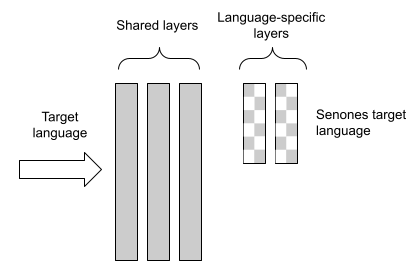
\includegraphics[scale=0.5]{imgs/Ours_final.png}
\caption{Multilingual transfer learning approach. Language-specific layers can be randomly initialized for a language not present during the MTL phase or use the corresponding pre-trained layers in case the target language was present during the MTL phase. Grey blocks are pre-trained during MTL phase.}
\label{fig:MLTL1}
\end{center}
\end{figure}


\subsection{Setup}
\label{section:corpus}
All experiments were conducted using five children corpora, each from a different language. Namely PFSTAR\_SWE, ETLTDE, CMU, LETSREAD and CHOREC. All those datasets have been described in section \ref{section:children_corpora}.%This section briefly presents each corpus and how it was used in the present study. In addition, more 
Table \ref{tab:statistics} presents statistics about the duration, number of utterances and language %can be found in Table \ref{tab:statistics}. 
Notice that in this work we have only used small datasets to better reflect the average size of the available children's speech corpora.

\begin{table}[ht]
\begin{center}
\begin{tabular}{llcc}
\hline
Corpus name & Language     & Train & Test  \\ \hline
\multicolumn{1}{l}{PFSTAR\_SWE} & Swedish             & 6030 utt  & 2879 utt  \\ 
\multicolumn{1}{l}{} &              & 04h00 & 01h48 \\\hline
\multicolumn{1}{l}{ETLTDE}      & L2 German   & 1445 utt &  339 utt \\ 
\multicolumn{1}{l}{}      &    &  04h41 & 01h06 \\ \hline
\multicolumn{1}{l}{CMU}         & English             & 3637 utt & 1543 utt \\ 
\multicolumn{1}{l}{}         &              & 06h26 & 02h45  \\ \hline
\multicolumn{1}{l}{LETSREAD}    & Portuguese & 3590 utt & 1039 utt \\ 
\multicolumn{1}{l}{}    &  & 12h00 & 02h30 \\  \hline
\multicolumn{1}{l}{CHOREC}      & Dutch               & 2490 utt & 575 utt  \\ 
\multicolumn{1}{l}{}      &                &  20h12 & 04h42 \\ \hline
\end{tabular}
\caption{Statistics on the different corpora of children's speech.}
\label{tab:statistics}
\end{center}
\end{table}

We employ the same experimental design as the prior experiment with adult data from section \ref{section:exp_setup} setup, where the acoustic model is divided in two. The first part is shared across all languages, whereas the second is language specific.
Furthermore, each corpus, i.e. each language, uses an independent language model and lexicon that is constant throughout all experiments in order to assess solely the acoustic model contribution.

\subsection{Multilingual-transfer learning experiment}

\begin{table*}[ht] 
\begin{center}
\begin{small}
\begin{tabular}{c|ccccc}

\hline
 & PFSTAR\_SWE & ETLTDE & CMU &  LETSREAD & CHOREC   \\  \hline
 \multicolumn{1}{c|}{Language} & \textit{Swedish} & \textit{German}  &  \textit{English}  & \textit{Portuguese} & \textit{Dutch}   \\ \hline
\multicolumn{1}{c|}{Single language} & 54.36\% & 44.69\%  &  21.26\%  & 26.88\% & 25.15\%    \\ \hline
\multicolumn{1}{c|}{MTL} & 54.95\% & 42.46\% & 23.01\% & 27.45\% & 25.10\%   \\ \hline
\multicolumn{1}{c|}{TL from PFSTAR\_SWE} & - & 42.23\% & 20.62\% & 26.47\% & 24.65\%   \\ 
\multicolumn{1}{c|}{TL from  ETLTDE}  & 53.60\% & -  &  20.90\% & 26.61\%  & 25.42\%        \\ 
\multicolumn{1}{c|}{TL from CMU}  & 52.83\%   & 41.54\%    & - & 26.49\% & 24.58\%   \\ 
\multicolumn{1}{c|}{TL from LETSREAD} & 52.50\% & 41.77\%  & 20.41\% & - & 24.60\%   \\ 
\multicolumn{1}{c|}{TL from CHOREC} & 52.20\% & 40.28\%    & 19.77\%    & 26.05\%   & -     \\ \hline
\multicolumn{1}{c|}{TL Average} & 52.78\% & 41.46\% & 20.43\% & 26.41\% & 24.81\%    \\ \hline
\multicolumn{1}{c|}{TL Best} & 52.20\% & 40.28\% & 19.77\% & 26.05\% & 24.58\%    \\ \hline \hline
\multicolumn{1}{c|}{MLTL} & \textbf{51.67\%} & \textbf{38.04\%} & \textbf{19.33\%} & \textbf{25.75\%} & \textbf{23.78\%}    \\ \hline \hline
\multicolumn{1}{c|}{MLTL-olo}  & \textbf{51.58\%} & 40.05\% & \textbf{19.67\%} & 26.20\% & \textbf{24.57\%} \\ \hline


\end{tabular}
\end{small}
\end{center}
\caption{WER results of multilingual-transfer learning and cross-lingual experiments. MTL: Multi-Task Learning, TL: Transfer Learning, MLTL: Multilingual Transfer Learning, MLTL-olo: Multilingual Transfer Learning one-language-out}
\label{tab:result-TL4epoch}
\end{table*}

Table \ref{tab:result-TL4epoch} presents the WER results of the multilingual transfer learning (MLTL) approach compared to three different methods: baseline, trained on each corpus individually for 4 epochs; Multi-task Training (MTL) alone, trained jointly using all corpora for 4 epochs
; Transfer Learning (TL) alone, adapted for the target language using in turn one of the other 4 baseline models as a source, leading to 4 results per target language. In addition, for clarity, we summarise the transfer learning scores with the average of the 4 scores and the best of the 4 for each target.

Firstly, it is important to emphasise that the baseline scores correctly reflect the different tasks the children were asked to perform and the corresponding amount of data available for each corpus. The best WER score, 21.26\% for CMU, can be explained by the reading-aloud-sentences task nature of this corpus. Thus, the language model can more easily compensate for the acoustic model errors. In addition, Chorec and LetsRead, as the largest corpora in our experiment, also yield relatively good results for children's speech recognition. On the other hand, ETLTDE and PFSTAR\_SWE show the worse WER results with 44.69\%  and 54.36\% WER, respectively. This can be explained by the amount of data available and by the language model which does not compensate as much as the CMU model. Especially for ETLTDE, since it is the only corpus that does not contain scripted text, but spontaneous responses. In addition, the age range of PFSTAR\_SWE children also plays a critical role in performance, since younger children generally yield worse performance scores \cite{TFchildren}.

Turning to multi-task learning, among all the approaches presented, only MTL fails to improve the baseline performance for almost all languages, which is in contradiction with\cite{TransferLF}.  However, it can be explained by the differences in terms of the size of the child's speech corpora used. The smaller the size of the corpora used, the more difficult it is to model the acoustic variation in the children's speech.


Concerning TL, all performance scores outperform their corresponding baseline, confirming that TL is an adequate method for children's ASR since it allows the system to be confronted with more children, thus with more variation. Precisely, table \ref{tab:result-TL4epoch} shows that the best pre-trained model for knowledge transfer is Chorec.
This makes sense since Chorec is the largest corpus, representing about 40\% of the total data used in our experiments.


Finally, MLTL shows an average relative improvement in WER of 7.73\%  compared to the baseline, slightly higher than the average (TL Avg) and the best (TL Best) transfer learning performance, with an average relative improvement of 4.50\% and 2.66\%, respectively. 

The strength of MLTL is that it can benefit both from MTL and TL, minimizing some of their associated weaknesses.
Attending to our results, MTL does not improve single language training. We believe that the unbalanced amount of data, the significant differences among data sets and the use of segmental optimization (lattice-free MMI) can partially explain these results. Nevertheless, we hypothesize that the multi-task objective leans the network towards 
better optimization of the lower layers, rather than optimizing the upper language-specific layers, can still be beneficial for TL.
Regarding TL, one can observe considerable performance variations depending on the pre-trained model used as the source model, probably due to a poorer initialisation of lower layers that is less efficient for TL. The MLTL experiments show that we can overcome these drawbacks by combining both MTL and TL, thus, validating the effectiveness of this approach for robust speech recognition of children.



\subsection{Cross-lingual validation}
\label{section:olo}

In the previous section, we saw that the MLTL approach yields better results than separate multi-task and transfer-learning frameworks.

To further validate the hypothesis that the shared lower layers are able to learn meaningful information about children's speech characteristics, regardless of the language, we perform a cross-language experiment following a leave one-language-out cross-validation setting. In this experiment, we keep one language out of the multi-task training and use it only during the TL phase to adapt the acoustic model parameters. 

We repeated this procedure for each corpus in our experiment. As in the previous experiment, we used 4 epochs for each learning phase. The last row of Table \ref{tab:result-TL4epoch} presents the results of the cross-language experiment.

For all corpora, the MLTL one-language-out (MLTL-olo) approach outperforms the baseline WER score with an average relative improvement of 5.56\%. Improvements are more important for the small corpora ETLTDE and CMU, with a  relative improvement of 14.88\% and 9.07\%, respectively. PFSTAR\_SWE does not benefit as much, with only 5.05\% relative improvement. This is mainly due to the age differences with the children in the other corpora used in the MTL phase. Indeed, the children in PFSTAR\_SWE are much younger (see section  \ref{section:corpus} for more details). Therefore, we conclude that the shared layers have learned the underlying multilingual features of children.

It is also interesting to compare MLTL-olo with the results of transfer learning alone. In both cases, the pre-trained models used have never seen the target language data. We observe that the results between the MLTL-olo and TL Best are extremely close, with small improvement with the MLTL-olo, only the best transfer learning model on LetsRead is slightly better than MLTL. This means that during multilingual training the system learned, at least, the best representation of the available children's characteristics. This is consistent with our hypothesis of the important role of the multilingual training phase in our two-step procedure.

\subsection{Summary and discussion}
%\label{section:conclusions}
In this work, we addressed the following research question: Does the two-step training strategy we propose in the current chapter outperform conventional single language/task training for children's speech, as well as multilingual and transfer learning alone. Our results provide a positive answer to this question, by showing that the limitations of MTL and TL can be overcome by the multilingual transfer learning approach, even in a low-resource scenario, leading to an average relative improvement of 7.73\%. Multilingual pre-training is also beneficial for transfer learning with an unseen language, with an average relative improvement of 5.56\%. Multilingual transfer learning thus seems to be an appropriate method to address children's speech recognition in a challenging context.

%In future work, it would be interesting to investigate the effect of a larger children corpus or an adult speech corpus in the multilingual learning phase, as this would allow the model to be more acoustically robust. In addition, it would be interesting to explore the effect of non-European languages, as previous works has shown an improvement by combining Madarin and English. Furthermore, a more detailed comparison between age groups on the systems' performance would be an interesting next step. Finally, assessing the importance of the nature of the task within the multi-task phase and transfer learning phase would also be a possible avenue for future research.

\section{Conclusion}
In this chapter, we look at the current state of the art for a Hybrid HMM-DNN speech recognition system for children. We illustrated that transfer learning is the most promising strategy for addressing children's ASR variability because it makes efficient use of the knowledge contained in the pre-trained source model. A pre-trained model that can be trained on both adults or children. The multi-task learning does not produce the greatest results alone, but we showed that the shared part of the model is capable of learning relevant information for all tasks jointly. Furthermore, we proposed in this chapter to combine these two approaches in our multilingual transfer learning system. Using the capacity of learning relevant information of the multi-task learning approach and the capabilities of efficient use of pre-existing knowledge from transfer learning. 







% If Printing on DOUBLE SIDED pages, the second page should be white.
% Otherwise, comment the following command:
\cleardoublepage{}
%
%Chapter 4
%% #############################################################################
% This is Chapter 4
% !TEX root = ../main.tex
% #############################################################################
% Change the Name of the Chapter i the following line
\fancychapter{End-to-End children automatic speech recognition}
\label{chap:e2e}
\cleardoublepage
\section{Introduction}
\label{chap:implement}
% End2End better and better
The growing popularity of deep learning has witnessed numerous successful applications in ASR. NIt was only recently, that end-to-end models have shown their capability to outperform hybrid HMM-DNN systems for a variety of speech recognition tasks, including children's ASR. The primary advantage of end-to-end speech recognition systems lies in merging the entire training process within a single neural network, thereby eliminating potential behavioral incompatibilities that may arise between independently trained modules.

However, the application of the end-to-end paradigm for children's ASR is a relatively recent development and has not been extensively explored, mainly due to the challenge of data scarcity in the context of children's speech \cite{gelin2021endtoend,sri_end2end,chen2020data,ng2020cuhk}. Additionally, end-to-end models often necessitate a larger number of parameters to achieve the desired robustness and flexibility. Consequently, training them on small datasets becomes increasingly challenging \cite{luscher2019rwth}. Despite these challenges, the exploration of end-to-end models holds promise for advancing the state-of-the-art in children's ASR.

%With the growing popularity of deep learning, numerous successful attempts to apply it to ASR have been made. It was only recently, that end-to-end models have shown their capability to outperform hybrid HMM-DNN systems for a variety of speech recognition tasks, including children's ASR. The major advantage of end-to-end speech recognition systems is the merging of the whole training process into a single neural network that eliminates the possibility of behavioural incompatibilities between modules that have been trained independently. However, because of the problem of children's data scarcity, the application of the end-to-end paradigm for children's ASR is relatively new and has not been extensively investigated \cite{gelin2021endtoend,sri_end2end,chen2020data,ng2020cuhk}. In addition, end-to-end models often require more parameters to provide such robustness and flexibility. As a result, training on small datasets becomes increasingly difficult \cite{luscher2019rwth}.

As mentioned in section \ref{section:SOTAE2E}, the recent increased interest in end-to-end speech recognition, has led development the  several architecture, encompassing recurrent neural networks \cite{soltau2016neural}, neural transducers \cite{battenberg2017exploring}, and the Transformer architecture \cite{vaswani2017attention}. Among these, the Transformer architecture stands out as it consistently delivers state-of-the-art results in large-vocabulary speech recognition, demonstrating its efficacy across both adult and children's speech domains \cite{gelin2021endtoend}.
%With the recent increased interest in end-to-end speech recognition, several architectures have been developed, including recurrent neural networks \cite{soltau2016neural} and neural transducers \cite{battenberg2017exploring}. However, one architecture stands out and consistently provides state-of-the-art results in large-vocabulary speech recognition for both adults and children, the Transformer.

This chapter will dives into more details of the Transformer design as well as the adapter transfer for children ASR, a  parameter-efficient transfer for Transformer models that we have recently proposed.
\section{Transformer model}
\label{sec:trans_archi}

\begin{figure}[ht]
    \centering
    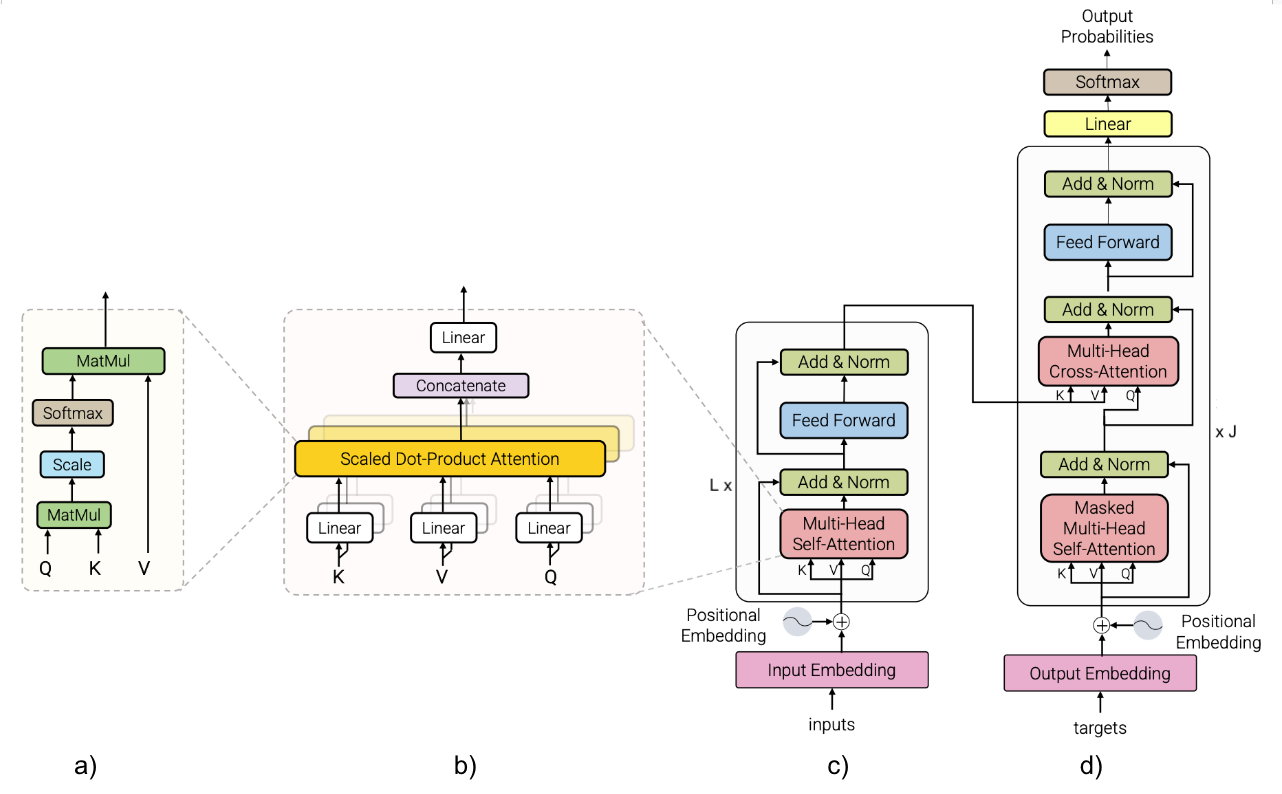
\includegraphics[width=1\textwidth]{imgs/transformer_archi.png}
    \caption{Architecture of the standard Transformer \cite{vaswani2017attention}. a) scaled dot-product attention, b) multi-head self-attention, c) Transformer-encoder, d) Transformer-decoder.}
    \label{fig:transformer_archi}
\end{figure}
% Explain transformer
Introduced in 2017 by Vaswani et al. \cite{vaswani2017attention}, the Transformer architecture is a sequence-to-sequence encoder-decoder model that relies solely on self-attention mechanisms, completely discarding the use of recurrence and convolutions. This design choice addresses challenges such as vanishing gradient issues commonly associated with recurrent neural networks. Another notable difference with recurrent neural networks is that the Transformer computes the dependencies between each pair of positions simultaneously, rather than one by one, by directly encoding the position in the sequence. This enables more parallelisation and therefore a faster training process.

Since its introduction, the Transformer architecture had a tremendous impact across various domains, including Natural Language Processing (NLP) \cite{Bert,brown2020language}, computer vision \cite{dosovitskiy2020image}, and speech processing \cite{dong2018speech}. The Transformer's capacity to capture intricate dependencies and patterns in sequences has established it as a popular architecture in the deep learning field, contributing to advancements and breakthroughs across various applications, such as ChatGPT \cite{bahrini2023chatgpt} or Dall-E \cite{ramesh2021zero}.
%First proposed in 2017 \cite{vaswani2017attention}, the Transformer architecture is a sequence-to-sequence encoder-decoder architecture that relies entirely on self-attention, eliminating recurrence, convolutions entirely and vanishing gradient issues. Another notable difference with recurrent neural networks is that the Transformer computes the dependencies between each pair of positions simultaneously, rather than one by one, by encoding the symbol position in the sequence. This, enables more parallelisation, resulting in faster training. Since its release, the Transformer architecture had tremendous impact in various areas, including NLP \cite{Bert}, computer vision \cite{dosovitskiy2020image}, and speech \cite{dong2018speech}.

The Transformer encoder-decoder architecture, as depicted in Figure \ref{fig:transformer_archi}, consists of an encoder (c) and a decoder (d). Prior to entering the encoder or decoder, both inputs and targets undergo processing through an embedding layer. This involves the use of learned embeddings to convert input tokens and output tokens into vectors of dimension $d_{\text{model}}$. 
% Positional embedding
Since the transformer model contains no recurrence and no convolution mechanisms, information about the relative or absolute position of the tokens must be injected in the sequence to allow the model to make use of the order of the sequence. To achieve this, information about the relative or absolute position of the tokens is obtained through the summation of the input/output embedding and the positional embedding. While various alternatives for positional encodings were used , Vaswani et al. \cite{vaswani2017attention} proposed the use of sinusoidal and cosine functions with different frequencies, as follows:
%Since the transformer model contains no recurrence and no convolution, in order for the model to make use of the order of the sequence, some information about the relative or absolute position of the tokens are injected in the sequence.
%The information about the relative position of the tokens in the sequence is given by the summation between the input/output embedding and the positional embedding. Although there are many choices of positional encodings, \cite{vaswani2017attention} proposed to use sine and cosine of different frequencies as follows:
\begin{align}
    PosEnc_{(pos,2i)} = \sin(pos/10000^{2i/d_{\text{model}}})\\
    PosEnc_{(pos,2i+1)} = \cos(pos/10000^{2i/d_{\text{model}}})
\end{align}
Where $pos$ is the current token or label position and $i$ is the dimension.
 

%Encoder
The encoder's primary objective is to transform the input sequence $X = x_1, \dots, x_T$ into a series of continuous representations $Z = z_1, \dots, z_T$. The encoder is structured as a stack of $L$ identical layers, each comprising two sub-modules: the multi-head self-attention (MHSA) and the position-wise fully connected feed-forward network (FFN). Each of these modules are followed by a normalisation with a residual connection.

%Decoder
Subsequently, the continuous representations $Z$ are fed into the decoder. The decoder is responsible for constructing an output sequence $Y = y_1, \dots, y_N$ one element at a time. At each time step, the decoder receives both the encoder outputs and the last decoder output in an auto-regressive manner. Similar to the encoder, the decoder is composed of a stack of $J$ identical layers. Nevertheless,in comparison to the encoder, the decoder encompasses a third sub-module, which performs multi-head attention (MHA) over the output of the encoder stack. The self-attention sub-module in the decoder stack is modified to prevent positions from attending to subsequent positions. This masking combined with a modified MHA prevents the attention to use subsequent positions, ensuring that the prediction at time-step $i$ solely depends on the previous $< i$ time-steps.


%The transformer encoder-decoder architecture is presented in figure \ref{fig:transformer_archi}, with c) the encoder and d) the decoder. The encoder's role is to transform an input sequence $X = x_1, \dots,x_T$ into a series of continuous representations $Z = z_1, \dots,z_T$ which are then fed into a decoder. The decoder, constructs an output sequence $Y = y_1, \dots, y_N$, one element at a time. At each time step, the decoder receives the encoder outputs together with the last decoder output, in an auto-regressive manner.
% Input embedding



%The encoder is composed of a stack of N identical Transformer layers. Each layer consists of a multi-head self-attention module and a feed-forward fully connected neural network module. Each of these modules are followed by a normalization with a residual connection.
%In comparison to the encoder, the decoder contains a third sub-layer, which performs MHA over the output of the encoder using the prior sub-layer of the decoder as the query. The decoder's inputs, which are targets during training and the previously decoded label during inference, are offset by one position. This combined with a modified MHA prevents the attention to use subsequent positions, ensuring that the prediction at time-step $i$ solely depends on the previous $< i$ time-steps.
%MHSA 
The MHA module relies on scaled dot-product attention \cite{vaswani2017attention}, as illustrated in Figure \ref{fig:transformer_archi}(a). Scaled dot-product attention focuses on determining how relevant a particular token is with respect to other tokens in the sequence and is defined as follows:

\begin{align}
\text{Attention}(Q, K, V) = \text{softmax}\left(\frac{QK^T}{\sqrt{d_k}}\right)V
\label{equation:attention}
\end{align}


Here, the input consists of queries $Q$, keys $K$ of dimension $d_k$, and values $V$ of dimension $d_v$. The dot product of the query with all keys is divided by $\sqrt{d_k}$, and the result passes through a softmax function to obtain attention weights. The attention weights are then multiply with the values. When $d_k$ is large, the scaling  $\frac{1}{\sqrt{d_k}}$ restrains the dot product from growing large in magnitude. Note that the Multi-Head Self-Attention (MHSA) is a specific case of MHA where $K$, $V$, and $Q$ are all the same input of the module.

Instead of performing a single scaled dot-product attention, the MHA module linearly projects $h$ times $K$, $V$, and $Q$ with different, learned, linear projections to dimensions $d_k$, $d_k$, and $d_v$ respectively. The attention function \ref{equation:attention} is then applied in parallel to each of the $h$ projected versions. The output of each of the $h$ attention functions, of dimension $d_v$, is concatenated and projected one final time, as depicted in Figure \ref{fig:transformer_archi}(b). Each of the $h$ attention functions is called a head, while the overall is called Multi-head attention (MHA) or Multi-Head self-attention (MHSA) if $K$, $V$ and $Q$ are the same. More formally:

\begin{align}
\text{MultiHead}(Q, K, V) = \text{Concat}(\text{head}_1, \dots, \text{head}_h)W^O
\end{align}
where
\begin{align}
\text{head}_i = \text{Attention}(QW_i^Q, KW_i^K, VW_i^V)
\end{align}
and the different projection matrices are $W_i^Q \in \mathbb{R}^{d_{\text{model}} \times d_k}$, $W_i^K \in \mathbb{R}^{d_{\text{model}} \times d_k}$, $W_i^V \in \mathbb{R}^{d_{\text{model}} \times d_v}$, and $W^O \in \mathbb{R}^{hd_{v} \times d_{\text{model}}}$.




%A MHA modules relies on the scaled dot-product attention \cite{vaswani2017attention}, illustrated in figure \ref{fig:transformer_archi}.a). Scale dot-product attention focuses on how relevant a particular token is with respect to other tokens in the sequence. And is defined as follows:
%\begin{align}
%    \text{Attention}(Q,K,V) = \text{softmax}(\frac{QK^T}{\sqrt{d_k}})V
%    \label{equation:attention}
%\end{align}
%Where the input consists of queries Q, keys K of dimension $d_k$ and values V of dimension $d_v$. The dot product of the query with all keys is each divided by $\sqrt{d_k}$, then passes through a softmax function to obtain attention weights on the values. When $d_k$ is large, the scaling  $\frac{1}{\sqrt{d_k}}$ restrains the dot product from growing large in magnitude. Note that the MHSA is a particular case of MHA where K,V and Q are all the input of the module.

%Instead of performing a single scaled dot-product attention, the MHA module linearly projects $h$ times K, V and Q with different, learned, linear projections to dimensions $d_k$,$d_k$ and $d_v$ respectively. On each of $h$ projected versions is performed the attention function \ref{equation:attention} in parallel. The output of each of the $h$ attention function, of dimension $d_v$ is concatenated and projected one last time as pictured in figure \ref{fig:transformer_archi}.b). More formally:
%\begin{align}
%    \text{MultiHead}(Q,K,V) = \text{Concat}(\text{head}_1, \dots, \text{head}_h)W^O \\
%    \text{where } head_i = \text{Attention}(QW_i^Q, KW_i^K, VW_i^V)   \nonumber
%\end{align}
%Where the different projections matrices are $W_i^Q \in \mathbb{R}^{d_{\text{model}}\times d_k}$, $W_i^K \in \mathbb{R}^{d_{\text{model}}\times d_k}$, $W_i^V \in \mathbb{R}^{d_{\text{model}}\times d_v}$ and $W^O \in \mathbb{R}^{hd_{v}\times d_{model}}$.


% FFN
Furthermore, in addition to the attention modules, each layer within the encoder and decoder encompasses a FFN module. This network is applied to each position separately and identically, and it consists of two linear transformations with a Rectified Linear Unit (ReLU) activation in between. While attention capture interdependencies between the element of the sequence regardless of their position, the FFN non-linearly transform each input token independently:

\begin{align}
    FFN(x) = max(0,xW_1 + b_1)W_2 + b_2
    \label{equation:FFN}
\end{align}
With $W_1 \in \mathbb{R}^{d_{model} \times d_{ffn}}$, $b_1 \in \mathbb{R}^{d_{ffn}}$, $W_2 \in \mathbb{R}^{d_{ffn} \times d_{model}}$ and $b_2 \in \mathbb{R}^{d_{model}}$. Typically $d_{ffn}$ is usually set to $4 \times d_{model}$.

\section{Conformer model}
\label{sec:conformer}
\begin{figure}[h]
    \centering
    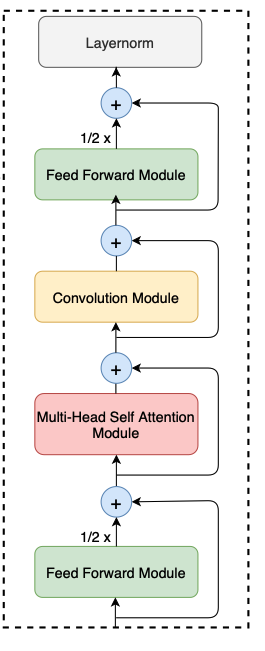
\includegraphics[scale=0.4]{imgs/ConformerLayer.png}
    \caption{Architecture of a Conformer layer}
    \label{fig:conformer_archi}
\end{figure}

\begin{figure}[h]
    \centering
    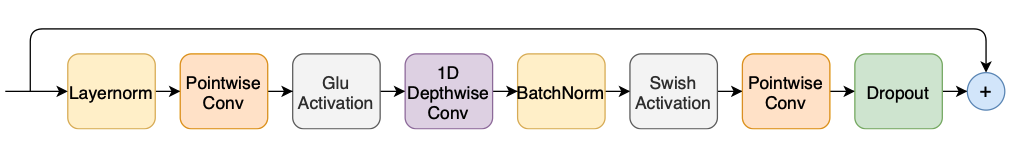
\includegraphics[width=1\textwidth]{imgs/ConvolutionModule.png}
    \caption{Convolution module in the context of a conformer layer}
    \label{fig:convModule}
\end{figure}
Transformers are recognised for their effectiveness in capturing global information within sequential tasks, thanks to the attention mechanism. Conversely, CNNs excel in capturing local features within data. To leverage the complementary strengths of both architectures, various approaches have been explored \cite{bello2019attention,yang2019convolutional}, and the Conformer architecture \cite{gulati2020conformer} stands out as a notable combination of Transformers and CNNs.

This combination involves incorporating CNNs into the conventional Transformer architecture, as depicted in Figure \ref{fig:conformer_archi}. Specifically, a Conformer block comprises four modules arranged sequentially: a FFN module, a MHSA module, a convolution module, and a second FFN module. Notably, the Conformer block features two FFN modules sandwiching the MHSA module and the Convolution module. This design is inspired by Macaron-Net \cite{lu2019understanding}, which advocates replacing the original FFN in the Transformer block with two half-step FFN modules—one before the attention layer and one after. Similar to Macaron-Net, half-step residual weights is employed for the FFN modules. More formally, for an input $x_i$ to a Conformer block $i$, the output $y_i$ of the block is defined as follows:

%While Transformers are known for their effectiveness in capturing global interactions within data, especially in sequential tasks, with the help of the attention mechanism, CNNs excel at capturing local features within data. Consequently, different appraoches tried to use combining Transformer and CNNs, among these the Conformer architecture was introduced to effectively combine the strengths of both Transformers and CNNs. This is achieved by integrating CNNs into the conventional Transformer architecture as shown in figure \ref{fig:conformer_archi}. More specifically, a Conformer block consists of four modules arranged sequentially: a feed-forward module, a self-attention module, a convolution module, and a second feed-forward module. It is important to note that the Conformer block contains two FFN modules sandwiching the MHSA module and the Convolution module, inspired by Macaron-Net, which proposes replacing the original feed-forward layer in the Transformer block into two half-step feed-forward layers, one before the attention layer and one after. As in Macron-Net, we employ half-step residual weights in our feed-forward (FFN) modules.  Mathematically, for input $x_i$ to a Conformer block $i$, the output $y_i$ of the block is:
\begin{align}
    \begin{split}
    \tilde{x_i} = x_i + \frac{1}{2}FFN(x) \\
    x_i^{\prime} =\tilde{x_i} + MHSA(\tilde{x_i}) \\
    x_i^{\prime\prime} = x_i^{\prime} + Conv(x_i^{\prime}) \\
    y_i = LayerNorm(x_i^{\prime\prime} + \frac{1}{2}FFN(x_i^{\prime\prime}))
    \end{split}
\end{align}

More specifically,the convolution modules , inspired by \cite{wu2020lite} and illustrated in Figure \ref{fig:convModule}., starts with a gating mechanism \cite{dauphin2017language} involving a pointwise convolution and a gated linear unit (GLU). Subsequently, a single 1-D depthwise convolution layer is employed. Finally, this 1-D depthwise convolution is followed by a Batchnorm iand then a Swish activation layer.


\section{Understand transfer learning efficacy for transformer based models}
% Explain motivation 
Motivated by the limited availability of children's speech data, TL emerges as a promising strategy to overcome this challenge in children's ASR. TL involves leveraging pre-trained models, typically trained on extensive out-of-domain datasets of adult speech, and adapting them to the specific characteristics of children's speech through a re-training phase using a smaller, in-domain dataset of children's speech. This approach has shown effectiveness in both traditional HMM-DNN approaches \cite{shivakumar2020transfer} and modern end-to-end ASR paradigms\cite{sri_end2end,gelin2021endtoend}. In chapter \ref{chap:Chapter3}, we presented the effectiveness of TL in improving HMM-TDNN-F models for both European-Portuguese and English children's speech.

While the end-to-end paradigm has become state-of-the-art for some children's datasets, particularly when adapted from pre-trained adult models using TL, it involves merging all components of traditional ASR (acoustic, pronunciation, and language models) into a single neural network. This unique neural network design leads to an increased number of parameters for end-to-end models. Therefore, there is a need to understand how these large pre-trained models behave when fine-tuned with limited downstream data. To address this, we propose to explore TL for children's speech using both Transformer models and the Conformer architecture, a variant of the Transformer specifically designed for speech tasks.


% Over param of transformer models
Investigating TL for large-size models is a crucial step in the development of robust children's ASR, given the widely acknowledged issue of overparameterisation in large Transformer-like models. For example, models like BERT \cite{Bert} have been widely recognized as overparameterised in various studies within the Natural Language Processing (NLP) field \cite{kovaleva-etal-2019-revealing,michel2019sixteen}. Overparameterisation occurs when models have more parameters than necessary for a given task. Notably, observations suggest that certain components or layers of the architecture can be removed without compromising performance and, in some cases, may even lead to slight performance gains \cite{kovaleva-etal-2019-revealing,michel2019sixteen,ye2023partial}. This recognition has fueled successful compression studies, including pruning and distillation techniques \cite{mccarley2019structured,sanh2019distilbert}.



% Overfitting of large model and loterry ticket hypothesis
Furthermore, the acknowledgment of overparameterisation in Transformer-based models raises questions about the efficiency and computational cost of these architectures. Larger models tend to be more prone to overfitting, as demonstrated in a study where an ASR model was scaled up to 10 billion parameters \cite{zheng22d_interspeech}. Overfitting can be a concern when applying TL as using a overfitted pre-trained model could potentially leading to decreased performances. Therefore, there is a need for ablation studies, involving the systematic removal of components of the model, to understand which parts contribute significantly to the performances \cite{shen2021partial,wang2021fine}. These studies, predominantly explored in the field of computer vision \cite{ye2023partial}, align with the Lottery Ticket hypothesis formulated by Frankle and Carbin \cite{frankle2018lottery}: \textit{``A randomly-initialized, dense neural network contains a subnetwork that is initialized such that—when trained in isolation—it can match the test accuracy of the original network after training for at most the same number of iterations''}.

Understanding the contribution of the different components of the large-size model not only helps optimise model architectures for specific tasks but also reduces the computational demands of training and inference. This is particularly relevant in scenarios with resource constraints, such as limited computational power, memory, and training data. 


% This work investigate it on children ASR
While these ablation works have been extensively studied in NLP and computer vision, this approach remains under-explored for speech tasks. Specifically, the recent successes of distilation and pruning techniques for speech models \cite{gandhi2023distilwhisper,chang2022distilhubert,peng23c_interspeech}, suggest that overparameterisation may also be present in ASR models. In the context of children's ASR, where data scarcity is a significant challenge, understanding and addressing overparameterisation could paves the way for the development of more tailored and efficient models, with improved performances. Notably, the Transformer and Conformer architectures have exhibited promising results in ASR applications, making them particularly compelling subjects for further investigation.


\subsection{Partial Transfer learning}
% Explain experiments
Our aim is to undertake a comprehensive exploration of TL, specifically on end-to-end ASR for children's speech. Notably, the previous research in this field has been focused on HMM-DNN models, as illustrated by the work of Shivakumar et al. \cite{shivakumar2020transfer}. It is noteworthy that the existing works on the end-to-end paradigm have only centered on the entire model fine-tuning, leaving a notable gap in the understanding of the impact of fine-tuning individual components.

Firstly, we perform a meticulous examination of the TL process, specifically isolating the effects on individual components of the Encoder and Decoder, in comparison to the fine-tuning of the entire model. The prevailing hypothesis asserts that the Encoder is  capturing acoustic information, while the Decoder more linguistic informations. Considering the important presence of acoustic variability in children's speech, our investigation extended to discern which layers of the Encoder are more relevant for achieving effective TL.

Subsequently, our focus shifts to delineating the distinctive contributions of modules within both the Transformer and Conformer architectures during the fine-tuning process of adapting a pre-trained adult model to children's speech. Within the Transformer model, a granular analysis will be conducted to asses the roles of the MHSA module, the FFN, and the normalisation layers independently. Similarly, within the Conformer model, we evaluate the significance of the MHSA, FFN, normalisation, and convolution modules. This exhaustive examination is meticulously designed to identify the components that play a pivotal role in fine-tuning.


\subsection{Experimental setup}
\label{section:methods_chapter4}

\subsection{Corpus}
\begin{table}[ht]
\centering
\begin{tabular}{c|c|c}
\hline
 Training & Validation     & Test   \\ \hline
60897 utterances  & 10044 utterances   & 4079 utterances \\ 
 566 speakers  & 79 speakers   & 91 speakers \\ 
 113 hours  & 18 hours   & 13 hours \\ \hline

\end{tabular}
\caption{My Science Tutor Children Speech Corpus statistics}
\label{tab:statistics_myst}
\end{table}
In this experiment, we decided to used  the Boulder Learning My Science Tutor (MyST) corpus, as detailed in section \ref{section:children_corpora}. This choice aligns with the nature of the task assigned to the children in the MyST corpus, which involves spontaneous speech. The the end-to-end paradigm, by encapsulating both the acoustic model and language model within the same network, requires careful consideration. Indeed, if the model is trained on a limited set of prompts, from a dataset focused on reading tasks for example, it may learn and overfit to those specific prompts, yielding unreliable results.

For the purposes of our experiments, we decided to remove all utterances shorter than one second and longer than 20 seconds and shorter than one second. Typically, utterances shorter than one second were found to predominantly contain silence alone, while those longer than 20 seconds were constrained by our GPU limitations. The details of the filtered corpora used in our work are presented in Table \ref{tab:statistics_myst}. 

%In this work, we decided to use the Boulder Learning My Science Tutor (MyST) corpus, described in section \ref{section:children_corpora} given the task assigned to the children, which is to speak spontaneously. Indeed, the end-to-end model encapsulates the acoustic model and language model in the same network. As a result, if we train a model with a restricted amount of prompts on a data set of reading tasks, the model will learn and overfit the prompts. Thus, yielding unreliable results. Furthermore, for the purposes of our experiments, we decided to remove all utterances shorter than one second and longer than 20 seconds. The details of the filtered corpora used in our work are presented in Table \ref{tab:statistics_myst}. 
\subsection{Implementation details}

% Transformer  and Conformer model description
All experiments were conducted using the SpeechBrain toolkit \cite{speechbrain}. The Transformer model encompasses 12 Transformer layers in the encoder and 6 Transformer layers in the decoder, all with a hidden dimension of 512. Similarly, the Conformer architecture featured 12 Conformer layers in the encoder and 6 Transformer layers in the decoder, with a hidden dimension of 512. Both configurations used 8 heads for all MHSA, a FFN hidden dimension of 2048, and a dropout rate of 0.1. These models were pre-trained on a large English adult speech corpus, specifically the LibriSpeech dataset \cite{librispeech}, and are publicly available\footnote{https://huggingface.co/speechbrain/asr-transformer-transformerlm-librispeech\\ https://huggingface.co/speechbrain/asr-conformer-transformerlm-librispeech}. Furthermore, for all experiments, the same Transformer language model was employed, trained on 10 million words from LibriSpeech transcriptions. Our training involved 30 epochs with a learning rate of 8e-5. Furhtermore, in line with findings of \cite{gelin2021endtoend}, a combination of CTC and Seq2Seq losses was used, with respective weights of 0.3 and 0.7.

% TODO Should the url being citation with "last check on XX/12/23"?

\subsection{Encoder-Decoder Transfer learning}
% Encoder - Decoder
\begin{table}
    \begin{center}
        \begin{tabular}{lcc}\hline
            Transformer    &   WER $\downarrow$    & Trained parameters  \\ \hline
            Full model          & 12.99\% & 71.5M   \\
            Encoder only & \textbf{TODO\%} & 37.8M  \\
            Decoder only & 15.95\% & 25.2M  \\ \hline \hline
            Conformer    &    & \\ \hline
            Full model          & 12.28\% & 109M   \\
            Encoder only & \textbf{11.24\%} & 75.9M  \\
            Decoder only & 16.94\% & 25.2M  \\ \hline 

        \end{tabular}
    \end{center}
    \caption{Encoder-Decoder experiment}
    \label{tab:EncoderDecoder}
\end{table}
Table \ref{tab:EncoderDecoder} summarises the results of the impact of isolating fine-tuning of the encoder and decoder components within Transformer and Conformer ASR models. For the Transformer model, using fine-tuning then entire model exhibits a WER of 12.99\% using 71.5 million parameters. Isolating the encoder component leads to a significant improvement in WER, with TODO\% WER with a reduced parameter count of 37.8 million. Parallely, fine-tuning the decoder underperform compared to both full model and Encoder only fine-tuning by achieving a WER score of 15.95\% training 25.2 million parameters. 

Turning to the Conformer model, the full model achieves a WER of 12.28\% with 109 million parameters updated. Isolating the transfer learning on the encoder component only  yields a remarkable improvement, resulting in a WER of 11.24\% with a parameter count of 75.9 million. Conversely, when the decoder only is fine-tuned the performances degrade with a higher WER of 16.94\% using a parameter count of 25.2 million. Notably, the Conformer architecture consistently outperform the Transformer across all configurations, emphasising its effectiveness for speech related tasks. In addition, these results underscore the important role of the encoder in both Transformer and Conformer ASR models, highlighting its importance in capturing the inherent variabilities in children's acoustics. It confirms that the acoustics variabilities represent the most important source of variabilities as suggested by \cite{TFchildren}.

% Layers wise
\begin{figure}
    \begin{center}
        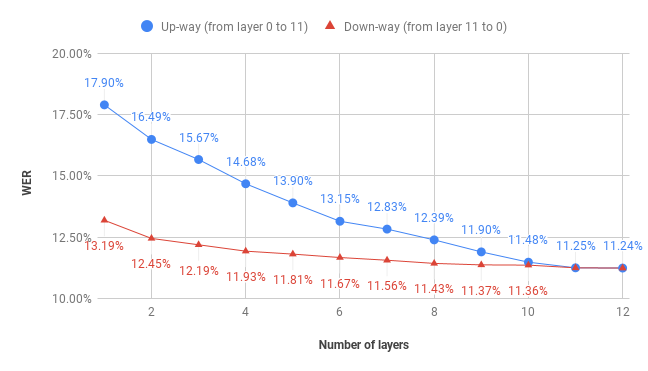
\includegraphics[scale=0.7]{imgs/layerTL.png}
    \end{center}
    \caption{Up-way and down-way transfer learning experiment}
\end{figure}
Recognising the important role of the Encoder in the fine-tuning process for children ASR, our investigation further look to determine the specific layers that are the most relevant during this TL process. To this end, we adopt a meticulous approach of fine-tuning the Encoder incrementally, adding one layer at a time. This step-by-step TL procedure is executed in each directionally, one commencing from the input layer while the other one from the output layer of the encoder,the up-way and down-way respectively. In other words, the up-way, incremental fine-tuning begining with the input layer and progressively incorporating subsequent layers towards the output layer. While, the down-way initiates fine-tuning from the output layer, systematically integrating preceding layers towards the input layer.
\subsection{Modules Transfer learning}
% Block wise
\begin{table}
    \begin{center}
        \begin{tabular}{lcc}\hline
            \textbf{Transformer}    & WER  $\downarrow$   & Trained parameters \\ \hline
            None & 25.04\% & -   \\
            Full model   & 12.99\% & 71.5M   \\ \hline
            Normalisation & 17.00\% & 57.9K  \\
            MHSA & 12.19\% & 25.2M  \\
            FFN    & \textbf{11.84\%}     &  37.8M \\ \hline \hline
            \textbf{Conformer}    &     & \\ \hline
            None & 21.75\% & -   \\
            Full model   & 12.28\% & 109M   \\ \hline
            Normalisation & 15.61\% & 63.7K  \\
            MHSA & 11.90\% & 15.7M  \\
            Convolution Module & 11.67\% & 9.7M \\
            FFN    & \textbf{11.11\%}     &  63M \\
            \quad $\hookrightarrow$ Module 1    & 11.44\%     &  25.2M \\
            \quad $\hookrightarrow$ Module 2    & 11.48\%     &  25.2M \\
            \quad $\hookrightarrow$ Up-linear ($W_1$)    & 11.47\%     &  31.5M \\
            \quad $\hookrightarrow$ Down-linear ($W_2$)    & 11.40\%     &  31.5M \\ \hline
        \end{tabular}
    \end{center}
    \caption{Modules fine-tuning experiment}
    \label{table:ModulesTL}
\end{table}
The results  of the transfer learning experiments, focusing on fine-tuning specific components of the Transformer and Conformer ASR models for children's speech, are presented in Table \ref{table:ModulesTL}. In addition of the WER evaluation metric, we also display the number of trained parameters. 

% Transformer
The baseline performance of the Transformer pre-trained model without any fine-tuning (corresponding to \textit{None} line) yields a WER of 25.04\%. In contrast, the fine-tuning of the full Transformer model exhibits a noteworthy improvement, achieving a WER of 12.99\% with 71.5 million parameters trained.

The fine-tuning of specific components reveals valuable observations. Applying normalisation alone results in a modest improvement WER of 17.00\% compared to keeping the pre-trained model, this using 57.9 thousand parameters. The MHSA module outperforms normalisation and full fine-tuning, achieving a WER of 12.19\% with a parameter count of 25.2 million. However, the most important improvement is observed with the FFN module, which attains a remarkable WER of 11.84\% with 37.8 million parameters. Remarkably, both MHSA and the FFN modules, when fine-tuned individually, already outperform the full model performance. This implies that the decrease in the number of parameters, coupled with the significance of these modules, may play a substantial role in the enhanced performances.

%Conformer
Turning to the Conformer model, the baseline WER without fine-tuning is 21.75\%, with no additional parameters. The full fine-tuning of the Conformer model improved performance, yielding a WER of 12.28\% with 109 million parameters.

Fine-tuning specific Conformer modules offers further granularity. First, the normalisation finetuning, in a similar way as observed in the Transformer configuration, yield a score of 15.61\% WER, with 63.7 thousand parameters. Then,  the MHSA module proves effective by already providing better result than the full full-tuning with a WER of 11.90\%, this by fine-tuning 15.7 million parameters. The convolution modules outperform the MHSA with a WER of 11.67\% with less parameters used, 9.7\%. Howver, as in the Transformer model, the FFN module stands out prominently, demonstrating a WER of 11.11\% with a parameter count of 63 million. Notably, the MHSA, convolution modules and FFN modules, when fine-tuned in isolation, surpass the performance of the full Conformer model.

% FFN wise
As FFN, consistently proved to be the most relevant component to fine-tune for children ASR, no matter the configuration. We decided to delve deeper into the FFN submodule. There is two way to see this subdivision, first using the macaron style of the Conformer FFn layer, including two modules, one before the MHSA and one after the convolution module will be respectively called Module 1 and Module 2. The second approach to subdivde the FFN layers would be to only look at the up-linear and down-linear, respectively $W_1$ and $W_2$ equation \ref{equation:FFN}. Module 1 and Module 2 achieve WERs of 11.44\% and 11.48\%, respectively, each by fine-tuning 25.2 million parameters. The Up-linear and Down-linear  submodules exhibit WERs of 11.47\% and 11.40\%, respectively, with parameter counts of 31.5 million. The subdivision of the FFN modules do not allow to perform better than their coupled usage. This show the importance of the full FFN modules in Transformer based end-to-end models. 

These comprehensive study not only highlight the importance of the various components within Transformer and Conformer ASR models but also underscore the effectiveness of fine-tuning only specific modules compared to the full model fine-tuning, especially the FFN module, in achieving improved performance.

\begin{comment}
\section{Adapters for Transformer based models}

Age-dependent acoustic models have shown promising improvements, as children's age is highly correlated with acoustic variability \cite{children_language_model2, reviewASRchildren}. In particular, some studies found that variability decrease with the age, reaching the adult level at 15 years old \cite{Acoustic_change_children}.
%End2End and transfer learning
In parallel, research on End-to-end (E2E) architectures has shown equivalent or even superior performance in a large number of speech recognition tasks compared to traditional hidden Markov models approaches \cite{hmm-end2end}. E2E architectures propose to combine different modules of the ASR pipeline into a single deep neural network (DNN), resulting in benefits to avoid error accumulation and mismatch between components.
However, for these models to work properly, they need to be trained with a large amount of data, which is not commonly available for children's speech. Thus, to overcome children's data sparsity issue for E2E models training, \cite{sri_end2end,gelin2021endtoend} successfully used transfer learning by fine-tuning an adult pre-trained model on children's speech.
%Motivation for adapter

In this work, we propose to apply adapter modules on top of an adult acoustic model as an alternative to the transfer learning strategy for automatic children's speech recognition. Adapters are a method recently proposed for Transformer-based systems that consist of a small set of additional layers that are attached to a source model \cite{houlsby,pfeiffer}. Adapters are typically less expensive both in terms of training speed and storage cost, which is a desirable property in the case of aiming at the development of children's age-dependent models.  In addition, adapters overcome the problem of catastrophic forgetting. Indeed, after using transfer learning, the source model is completely overwritten by the newly trained weights, leading to a drop of performance on the source task. Whereas in adapter transfer, the backbone model remains frozen, thus preserved if adapter layers are removed. Adapters are therefore very practical in the context of small device computing where it can be expensive to load and store a large number of models for adults and children of different ages. Finally, in this work, we also propose a novel version of adapter layers inspired by variational auto-encoders (VAE)\cite{VAE}, so-called variational adapters or Vadapters. We hypothesize that the ability of VAEs to estimate variability can be applied in adapters to make them more suitable for parameter-efficient automatic children's speech recognition.



 %The structure of this work is organized as follows. Section \ref{section:SOA} reviews end-to-end ASR and adapters. In Section \ref{Vadapters}, we introduce our Vadapter architecture for children adapter transfer. The experimental setup is described in Section \ref{section:methods}. Section \ref{section:exp} presents  experimental results for the different adapter architectures. Finally, in Section \ref{section:conclusions} we conclude this paper and present potential perspectives for future work.


\subsection{Related work}
\label{section:SOA}
\subsubsection{Transformer model for children ASR}
% Motivation children E2E
Recently, E2E-based ASR models have demonstrated their ability to achieve state-of-the-art performance on a wide variety of speech recognition tasks \cite{hmm-end2end}. This fact motivated the assessment and comparison of different E2E architectures for children ASR \cite{sri_end2end,gelin2021endtoend}. These works found that Transformer-based architectures, described in the previous section \ref{sec:trans_archi}, yield the best results when an adult pre-trained model is fine-tuned for children using transfer learning with the help of the joint attention and CTC objectives \cite{First_End2End}. Usually, these two objectives are combined  as follows:
% Transformer 
%Transformers were first introduced in Natural Language Processing (NLP) for machine translation task \cite{vaswani2017attention}. Due to its success, it has been used in many other areas such as computer vision \cite{VIT}, language understanding \cite{Bert} and speech  \cite{dong2018speech}. Transformer is a neural sequence transducer based on an encoder-decoder architecture that relies solely on attention mechanism. Acoustic features are given to the encoder that maps them into a high-level representation. The encoder output is then fed to the decoder that predicts tokens, usually characters. As showed by \cite{gelin2021endtoend}, the best way to train and infer children's speech by using Transformer is by jointly using the attention objective with a Connectionist Temporal Classification (CTC) objective \cite{First_End2End}. Usually, attention and CTC objectives are combined  as follows:
\begin{equation} \label{equa:loss_asr}
    \mathcal{L}_{ASR} = \lambda_{ctc} \mathcal{L}_{ctc} + (1- \lambda_{ctc})\mathcal{L}_{s2s}
\end{equation}
where $\mathcal{L}_{ctc}$ and $\mathcal{L}_{s2s}$ are the CTC and attention losses, respectively. A hyper-parameter $\lambda_{ctc} \in [0,1]$ is used to control contribution of each loss. 
\subsubsection{Adapters}
\begin{figure}[t]
\begin{center}
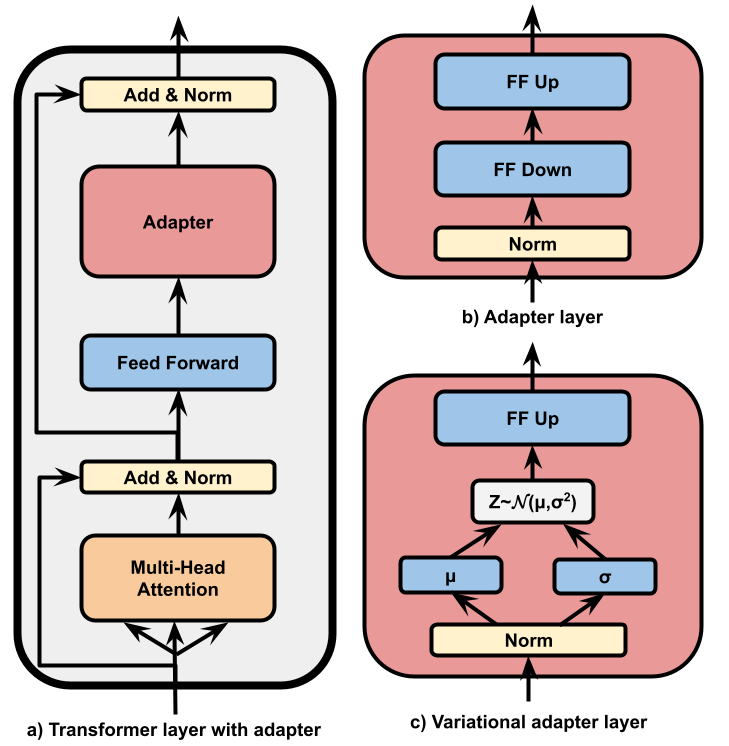
\includegraphics[scale=0.3]{imgs/Adapters.png}
\caption{a) Example of a Transformer layer with an adapter layer (adapted from \cite{pfeiffer}); b) Adapter layer; c) Vadapter layer}
\label{fig:all}
\end{center}
\end{figure}

% Adapters
Adapters were first introduced in the NLP field, motivated by the need for a parameter-efficient adaptation to fine-tune large models, like Transformer, on various text classification tasks \cite{houlsby}. They are a simple alternative to full model fine-tuning, as they involve only a small number of newly inserted parameters at each layer of the transformer.
While different positions have been proposed \cite{houlsby,pfeiffer}, they are generally plugged after the feed-forward layer (see Figure \ref{fig:all}.a). The key idea for training adapters is to freeze the backbone model's parameters and only update the adapter's parameters. Adapter modules are based on a bottleneck architecture (projection-down followed by a projection-up) as shown in Figure \ref{fig:all}.b.  Adapters solve a number of drawbacks associated with full model fine-tuning, such as parameter efficiency, faster learning iterations and a highly modular design

Since it was first proposed, adapters have been successfully used in a wide range of NLP tasks such as language understanding \cite{pfeiffer} and neural machine translation \cite{philip2020monolingual}. Some researchers proposed to use adapters for ASR tasks, such as in multilingual ASR \cite{kannan2019large}. More recently, \cite{tomanek2021residual} studied adapters for atypical speech, in particular pathological and accented speech. More recently, \cite{fan2022draft} proposed to use adapters inside of self-supervised models for children ASR by refining the whole model together with the weights of the adapters. Our work differs because our aim is to update only the adapters' weights in order to keep both the parameter efficiency and modular properties of adapters.

\subsubsection{Variational Auto-Encoders}
Variational auto-encoders (VAE) \cite{VAE} are a probabilistic generative models, that has been successfully applied in different speech tasks such as transformation \cite{vae_transformation} and enhancement \cite{vae_enh}. The main strength of VAE is their ability to learn a smooth representation of the latent space. Indeed, rather than producing a single value to describe each element of the latent space, as a standard auto-encoder, VAE provides a probability distribution: 
\begin{equation}
    p_{\theta}(\vb{x},\vb{z}) =  p_{\theta}(\vb{x}|\vb{z}) p_{\theta}(\vb{z})
\end{equation}
where $\vb{x}$ is the observed data generated by a random process using latent data $\vb{z}$ and $\theta$ denotes the distribution parameters. In this model, the likelihood function $ p_{\theta}(\vb{x}|\vb{z})$ quantifies   how the generation of $\vb{x}$ is conditioned by $\vb{z}$, while the prior $p_{\theta}(\vb{z})$ is used to regularize the latent data $\vb{z}$. Typically, a standard Gaussian distribution is used for the prior distribution
\begin{equation}
    p_{\theta}(\vb{z}) = \mathcal{N}(\vb{z}; 0, I)
\end{equation}
while the likelihood is defined as a multivariate Gaussian distribution:
\begin{equation}
     p_{\theta}(\vb{x}|\vb{z}) = \mathcal{N}(\vb{x}; \mu_{\theta}(\vb{z}), \sigma^2_{\theta}(\vb{z}))
\end{equation}
where $\mu_{\theta}(\vb{z})$ and $\sigma^2_{\theta}(\vb{z})$ are obtained using $\vb{z}$. However, since the posterior distribution $p_{\theta}(\vb{x}| \vb{z})$ is intractable, it is approximated with the auxiliary distribution $q_{\phi}(\vb{z}| \vb{x})$ that plays the role of an encoder:
\begin{equation}
    q_{\phi}(\vb{z}|\vb{x})= \mathcal{N}(\vb{z}; \Tilde{\mu}_{\phi}(\vb{x}), \Tilde{\sigma}^2_{\phi}(\vb{x}))
\end{equation}
 We also want to ensure that the approximate posterior $q_{\phi}(\vb{z}|\vb{x})$ and the true posterior $ p_{\theta}(\vb{z}|\vb{x})$ are similar by minimizing the Kullback-Leibler (KL) divergence between the two distributions. 
\begin{equation} \label{equa:minKL}
     \min KL(q_{\phi}(\vb{z}|\vb{x})|| p_{\theta}(\vb{z}| \vb{x}))
\end{equation}
It is possible to minimize expression (\ref{equa:minKL}) by maximizing the following expression as shown in \cite{vae_transformation}:
\begin{equation}
    \mathbb{E}_{q_{\phi}(\vb{z}| \vb{x})} \log p_{\theta}(\vb{x}|\vb{z}) - KL(q_{\phi}(\vb{z}|\vb{x})|| p_{\theta}(\vb{z}))
\end{equation}
Where the first term is the reconstruction error and the second term a regularisation. %Generally, we choose $p_{\theta}$ to be a standard normal distribution $\mathcal{N}(0,1)$.

Thus, the VAE loss function can be define as followed:
\begin{align}
\mathcal{L}_{VAE} & = \mathcal{L}_{recons}+ \mathcal{L}_{KL} \\
                  & = \mathcal{L}_{recons}+ \sum_j KL((q_{\phi}^{(j)}(\vb{z}|\vb{x})|| p_{\theta}(\vb{z}))
\end{align}
for each dimension $j$ of the latent space. 

\subsection{Variational adapters}
\label{Vadapters}
% Motivation (latent space more continuous)
Adapters and auto-encoders (AE) share a similar encoder-decoder structure. Although the purpose of these two architectures is different, the role of their encoders is similar: map relevant characteristics of the input into a unique latent vector. On the other hand, their architecture differs in the decoders: AEs use the decoder to reconstruct the input, while adapters project the information contained in the latent vector to be processed by the next layer. Consequently, adapters suffer from the same problems as AEs, a poor capability to model variability.
In order to be more robust to the high variability of children's speech, we propose to represent each latent value in probabilistic terms. To this end, we propose Vadapter, a new adapter architecture in which the encoder structure of the adapter is replaced with the structure of a VAE's encoder as shown in Figure \ref{fig:all}.c.    

Consequently, during training, instead of a down-projection that maps the input into the latent representation, we now have two branches, producing the mean $\mu$ and variance $\sigma$. During inference, $\mu$ is used directly as a deterministic latent vector, discarding $\sigma$. We hypothesise that this deterministic inference allows Vadapters to capture variability in the $\sigma$ branch while keeping the $\mu$ more robust. In addition, dropping the $\sigma$ branch during inference keeps the number of parameters equivalent to normal adapters, thus preserving the parameter efficiency.

Similarly to VAEs, the regularisation term which ensures that the distribution of $q_{i}(\vb{z}| \vb{x})$ for each Vadapter at layer $i$ is similar to the standard normal distribution $p(\vb{z})$ is required. However, as there are many Vadapter layers we normalise the sum of all regularization terms by the number of Vadapter layers: 
\begin{equation}
    \mathcal{L}_{KL_{all}}  = \frac{\sum_L^iKL(q_{i}(\vb{z}|\vb{x})|| p(\vb{z}))}{L} \\
\end{equation}
where $L$ is the total number of Vadapters in the model. 
Then, we inject this regularisation loss into the E2E ASR loss defined in equation (\ref{equa:loss_asr}) as follows:
\begin{equation}\label{loss}
    \mathcal{L}_{ASR} = \lambda_{ctc} \mathcal{L}_{ctc} + (1- \lambda_{ctc})\mathcal{L}_{s2s}  + \beta \mathcal{L}_{KL_{all}} 
\end{equation}
where $\beta$ is an hyper-parameter to control the regularization's contribution.


\subsubsection{Experiments description}
In our first experiment, we will attempt to determine which component of the transformer model is most important to ASR children. As a result, this information will be used to determine the best location of the adapters in the transformer layer. Indeed, the adapter should come after the most important component since it will project the output of that component into the expected transformer space. In order to do this, we studied the role of each transformer layer sub-module by fine-tuning one or two of them with the children's speech data.


% Experiments description
Secondly, we analyze the performance of adapters in three scenarios: i) Adapters in all layers of the E2E model, ii) adapters only  present in the encoder layers, and iii) adapters only in the decoder layers. These experiments are motivated by the fact that the encoder is closely related to the acoustics generating a high-level representation of speech, while the decoder generates output tokens related to the linguistic domain. The objective is then to evaluate which components, the encoder  (acoustics) or the decoder (linguistics), benefit more from the adapter transfer.
In order to compare our new architecture with traditional adapters, we reproduce the three scenarios mentioned above by replacing the adapters with our Vadapters. Furthermore,  we evaluate the combination of Vadapter and traditional adapter in two scenarios, Vadaper in the encoder and adapter in the decoder, and vice versa.

\subsection{Results}
\label{section:exp}

\subsubsection{Transfer learning experiments}
\begin{table}[ht]
\centering
\begin{tabular}{lcc} \toprule
Fine-tuned part & WER $\downarrow$  & Trained parameters\\\hline
None & 25.04\% & - \\
Full model & 13.50\% & 71.5M\\ \hline
Norm & 18.08\% & 57.9K\\
MHA & 13.40\% & 25.2M \\
FFN & \textbf{12.57\%} & 37.8M \\ \hline
MHA + FFN & 12.78\%  & 63.0M\\
Norm + FFN & 12.92\% & 37.9M \\
Norm + MHA & 13.52\%  & 25.3M\\ \hline
\end{tabular}
\caption{Results of the fine-tuning on part of the model only}
\label{tab:result_TL_transformer}
\end{table}
Table \ref{tab:result_TL_transformer} shows results of the transfer learning on sub-modules of the Transformer model. Fine-tuning all the transformer's parameters, in the same way as the previous work \cite{sri_end2end,gelin2021endtoend}, gives better results than using the model trained only on adult data with 13.76\% compared to 25.04\% WER respectively. The fine-tuning of all normalisation weights improved the score compared to the adult model with 18.04\% but still under-perform compared to the full fine-tuning. Thus, the normalisation contribution in the children's transfer learning is limited. In contrast, fine-tuning the MHA or FFN yields better, results compared to the full transfer learning with 13.40\% and 12.57\% WER respectively. While always outperforming a full model update, the use of transfer learning on a combination of different model components reduces performance when compared to FFN alone. Transfer learning becomes more difficult by updating the weights of all components of the transformer as well as the non-transformer weights (i.e., Convolution blocks and embedding blocks), which explains why the entire fine-tuning produces worse results. In conclusion, FFN modules are the most relevant to fine-tune using transfer learning. This is because transformer feed-forward layers are key-value memories \cite{geva2020transformer}, where each key correlates with patterns in the training examples, and each value produces a distribution over the outputs. Consequently, adapters should be placed after the FFN sub-modules in order to achieve better results. This is consistent with Pfeiffer's work for NLP tasks \cite{pfeiffer}.

\subsection{Adapters and Vadapters results}
\begin{table}[t]
\begin{tabular}{ccc}
\hline
 Method & WER     & Trained parameters   \\ \hline
\multicolumn{1}{l}{No fine-tune} & 25.04\%   & - \\ 
\multicolumn{1}{l}{Fine-tune} & 13.50\% & 71.5M \\ \hline
\multicolumn{1}{l}{Adapter}  &   14.33\% & 4.8M  \\ 
\multicolumn{1}{l}{Adapter encoder only }    & 14.56\% & 3.2M  \\ 
\multicolumn{1}{l}{Adapter decoder only} & 20.10\%      & 1.6M  \\ \hline
\multicolumn{1}{l}{Vadapter} & 14.19\%     & 7.1M (4.8M)  \\
\multicolumn{1}{l}{Vadapter-enc + Adapter-dec } & 14.05\%     & 6.3M (4.8M)  \\
\multicolumn{1}{l}{Adapter-enc + Vadapter-dec } & 14.35\%     & 5.5M (4.8M)  \\
\multicolumn{1}{l}{Vadapter encoder only} & 14.51\%     & 4.7M (3.2M)  \\ 
\multicolumn{1}{l}{Vadapter decoder only} & 20.23\%     & 2.4M (1.6M)  \\ \hline

\end{tabular}

\caption{Results of the different approaches; In parenthesis are shown the number of parameters needed for inference after dropping the $\sigma$ branch.}
\label{tab:res}
\end{table}
\subsubsection{Adapters for children ASR}
Table \ref{tab:res} presents the word error rate (WER) results of the different approaches.
Firstly, the pre-trained Transformer adult model without any adaptation gives the worst result, with a WER of 25.04\%, while adult performances on Librispeech corpus are usually less than 6\%. 
This result shows the impact of the variability in child speech.
% ALBERTO: This result shows the impact of the variability in child speech. : DONE
Secondly, the adaptation of all 71.5 million parameters for children's speech resulted in a considerable improvement, with 13.50\% WER. This result correctly reflects the state-of-the-art performance obtained in the literature for the MyST corpus \cite{sri_end2end}. 
Regarding adapters, similarly to previous work in NLP \cite{houlsby} and ASR \cite{tomanek2021residual}, we observe that they perform slightly worse than fine-tuning, with a score of 14.33\% WER. However, it is important to note that adapters require less than 10\% of all parameters of the full fine-tuning. We also investigate adapter transfer for encoder and decoder only. Table \ref{tab:res} shows that adapters are more relevant when plugged into the encoder with 14.56\% WER while compared to the decoder with 20.10\% WER. This result confirms that acoustic variability plays a critical role in the degradation of children ASR performance \cite{shivakumar2020transfer}. 

Additionally, we also evaluated how different adapter hidden-dimension, i.e. the number of parameters, influence the speech recognition performance compared to the fine-tuning model.
Figure \ref{fig:ratio} displays the relative WER delta over the ratio of trainable parameters compared to the fine-tuned model. As a reference, the relative WER delta of the adult model with respect to fine-tuning is 85.5\%.
% ALBERTO: Add here: "As a reference, the relative WER delta of the adult model with respect to fine-tuning is 85.5\%.": Done
%We observe that the delta increases as the number of trainable parameters decreases.
We observe that the performance difference between fine-tuning and adapters decreases as the number of trainable parameters increases.
% ALBERTO: This observation is in reverse order of the Figure. I think it would be more clear so say: "We observe that the performance difference between fine-tuning and adapters decreases as the number of trainable parameters increases."
% ALBERTO: Can this figure show 2 constant lines? The fine-tuning performance and the adult model performance? Because this will allow saying something like: "While with only 2\% of the trainable parameters, adapters manage to surpass by a large margin the source model performance, adapters need a minimum amount of parameters to get close to the fine-tuning performance" Then, the 2 following sentences disappear and you would continue in "Nevertheless, ...": DONE
While with only 2\% of trainable parameters, adapters manage to surpass by a large margin the source model performance, adapters need a minimum amount of parameters to get close to the fine-tuning performance. Nevertheless, adapter transfer outperforms full fine-tuning, when the number of parameters used is around 30\% of the number of the entire model. There is therefore a trade-off between performance and parameter efficiency. A similar observation has been made in \cite{fan2022draft}.
%This degradation can be explained by the fact that in order to process children's speech, adapters need a certain amount of parameters. The model cannot be robust to children's speech variability when there are not enough parameters.

\begin{figure}[t]
\begin{center}
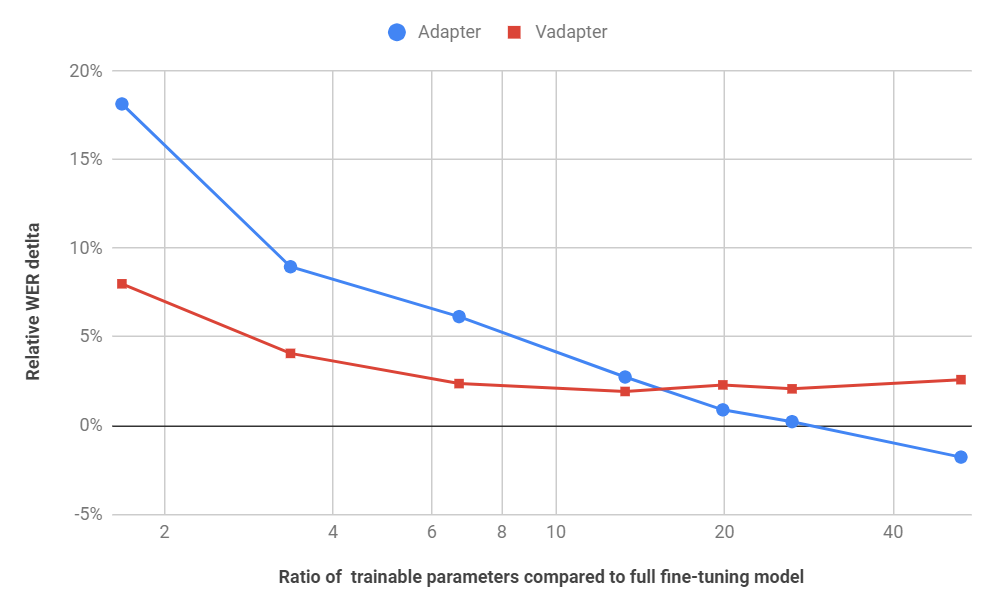
\includegraphics[scale=0.3]{imgs/ratio_delta.png}
\caption{Relative WER delta over the ratio (\%) of trainable parameters compared to full fine-tuned model.}
\label{fig:ratio}
\end{center}
\end{figure}
\vspace{-0.35cm}
\subsubsection{Variational-adapters}
Concerning the Vadapter architecture, with the exception of the cases where the Vadapters are placed in the decoder, all the scores are higher than their conventional counterpart, approaching the full fine-tuning score. The best configuration, Vadapter in the encoder and adapters in the decoder, reaches 14.05\% WER. In the same way, as for the conventional adapters, we can see that the Vadapters are more advantageous when placed in the encoder since the score is 14.51\% WER for Vadapters in the encoder only and 20.23\% WER for the decoder only. We believe that this is because Vadapters are designed to be more robust to acoustic variability, 
% ALBERTO: "We believe that this is because Vadapters...": Done
which is mainly present at the encoder level. Thus, the Vadapters in the decoder does not manage to improve the score of their conventional counterpart. 

Thus, we tested several possible combinations between Vadapter and adapters. We observe that the configurations with Vadapters in the encoder are giving the best results, with 14.19\% WER for Vadapters in both the encoder and the decoder, as well as 14.05\% for Vadapters in the encoder and adapters in the decoder. However, when Vadapters are placed in the decoder in combination with adapters in the encoder the result is not as good as adapters everywhere with 14.35\% WER. We believe again that this is due to the variability being more present in the acoustic than in the linguistic component.
% ALBERTO: "We believe again that this is due to ...: Done

Finally, as shown in Figure \ref{fig:ratio}, Vadapter outperforms conventional adapters when the number of parameters is less than 15\% of the full model. Indeed, the Vadapters are always under 10\% relative WER delta compared to full fine-tuning and reach under 5\% with less than 4\% of the ratio of trainable parameters, where conventional adapters start above 15\% relative WER delta and need more than 10\% of the ratio of trainable parameters to be under 5\% relative WER delta. These results confirm the proposed Vadapter architecture as a more convenient alternative for parameter-efficient transfer learning. However, when the number of parameters increases,  the results drop compared to conventional adapters. We hypothesize that this is due to the more complex and subject to variability sampling  of $\vb{z}$ during Vadapters training.


\subsection{Discusion}
\label{section:conclusions}
% Train age dependent variational-adapter and use AdapterFusion
In this work, we demonstrate the usefulness of adapter transfer in the context of children's speech. With less than 10\% of the total number of fine-tuning parameters, adapters are able to efficiently model children's speech. Noticeably, the adapter performance approaches fine-tuning, as the number of parameters increases. Furthermore, our Vadapter architecture outperforms conventional adapters in terms of acoustic variability robustness in a parameter-efficient setting. Using a combination of Vadapters in the encoder and conventional adapters in the decoder allows for further improvement, getting closer to the fine-tuning performance while keeping a small number of parameters.  This seems to demonstrate their effectiveness in modelling highly variable data, such as children's speech.
%This work is our first step towards the development age-dependent E2E ASR.
%In future work, we would like to train age-dependent adapters %and fuse them using attention.
%as well as investigate the behavior of new adapter architectures on children's speech.
\end{comment}
\section{Summary}
We covered the state-of-the-art for end-to-end children's speech recognition in this chapter. Particularly, the usage of the Transformer architecture in conjunction with transfer learning. In a similar way as chapter \ref{chapter:Hybrid}, to avoid a drop in performances attributable to an acoustic mismatch between children and adults, the end-to-end model should be trained with children's data. In contrast to previous work, we demonstrated that fine-tuning only a portion of the transformer modules, particularly the FFN sub-module, yields better results since it serves as a key-value memory. As a result, we placed our adapter subsequent to it. The adapter's role is to accomplish knowledge transfer, which is related to transfer learning. Rather than updating the complete model's weights, we just tweak an extra module, hence fewer parameters. This adapter transfer achieves almost identical results as the entire model fine-tuning. In addition, adapters are useful in the context of customized models, where training and storing a whole model for each age group or each child can be expensive and time-consuming.

In addition, we proposed the variational adapter, a variant of the traditional adapter based on variational auto-encoders. Compared to the adapter, which takes a bottleneck encoder-decoder structure with a linear layer as encoder and a linear layer as decoder, the variational adapter's encoder consists of two branches, $\mu$ and $\sigma$. The outputs of these two branches are used as the mean and variance vector to sample the input of the decoder. By doing so, we enforce the adapter's input variability to be contained in the $\sigma$ branch. A branch which is suppressed during inference. As a result, we reduce input variability while maintaining the same size as standard adapters.
% If Printing on DOUBLE SIDED pages, the second page should be white.
% Otherwise, comment the following command:
%\cleardoublepage{}
%
%Chapter 5
%% #############################################################################
% This is Chapter 5
% !TEX root = ../main.tex
% #############################################################################
% Change the Name of the Chapter i the following line
\fancychapter{Exploring Parameter-Efficient Strategies in Transfer Learning for Children-Focused ASR Systems}
\label{chap:5}
\cleardoublepage

%\section{Introduction}
The use of increasingly larger models coupled with the abundance of massive datasets is driving rapid advancements in many domains of machine learning, encompassing \ac{NLP} \cite{brown2020language} and computer vision \cite{ramesh2021zero}. In the context of \ac{ASR}, this trend of scaling up models is exemplified by state-of-the-art models such as Whisper \cite{radford2023robust} and HuBERT \cite{hsu2021hubert}, where the number of parameters can exceed 1 billion. Research has underscored the interconnected nature of the training dataset size and the number of model parameters, identifying them as mutual bottlenecks that influence the performance of machine learning models \cite{Kaplan2020ScalingLF}. This observation accentuates the significance of scaling these two dimensions in tandem for the development of more robust and effective \ac{ASR} models. Typically, to scale up the model size a combination of an increased number of layers and an expansion of the model's hidden dimensions are used \cite{zheng22d_interspeech}.

However, the challenge arises when only a limited amount of data is available, making it challenging to train these large models from scratch, as highlighted by recent studies \cite{sri_end2end, gelin2021endtoend}. Hence, as discussed in the preceding chapters, \ac{TL} emerges as a well-established and effective paradigm to tackle to problem of limited dataset. Nevertheless, despite its efficacy, we emphasised certain limitations that may potentially impede the performance of fine-tuning. Specifically, attempting to fine-tune these large models using a downstream dataset limited in size can be challenging, as shown in Chapter \ref{chap:4}. Indeed, in addition to being an expensive process, using a small amount of data on such a large model could potentially result in overfitting. This issue necessitates careful consideration, particularly in light of the recent evolution towards ever-growing pre-trained model sizes. Additionally, even following the last chapter's findings where only specific parts of the model were fine-tuned, the different parts of the model are intricately linked to the overall model size. For example, \ac{FFN} modules usually represent a substantial portion, between 50\% to  70\% of the total number of parameters. This insight underscores the persistence of the challenge associated with model size, even when fine-tuning only specific components. Finally, \ac{TL} on large amounts of parameters is memory-storage-inefficient, especially when there is a need to store replicas of all the models's parameters for many different small tasks.

Consequently, there is a growing need for more \ac{PETL} as lightweight alternatives to \ac{TL}. Among the approaches introduced by the research community, residual Adapter modules stand out as the most popular and promising \cite{houlsby, pfeiffer}. Specifically tailored for Transformer-based systems, Adapters integrate a compact set of additional layers into a pre-trained frozen source model. This design enables Adapters to enhance computational efficiency, resulting in faster training and addressing the challenge of catastrophic forgetting. Diverging from conventional \ac{TL} methods, where the source pre-trained model's weights are entirely replaced, Adapter-transfer maintains the integrity of the backbone model. Therefore, when the Adapter modules are removed, the initial pre-trained model remains unchanged. This preservation of the backbone model is a crucial advantage as it offers increased flexibility. Furthermore, owing to their limited number of trainable parameters, Adapters demonstrate a decreased susceptibility to overfitting, thereby contributing to improved generalisation performance for smaller training datasets.

 In this chapter, motivated by the promising characteristics of Adapters, we will investigate their application in the specific context of children's \ac{ASR}. The study will encompass the examination of diverse Adapter configurations within both Transformer and Conformer architectures. The investigation aims to unveil the potential for creating a model that optimally balances parameter efficiency and recognition accuracy. Additionally, we propose a novel approach, where speaker-group-based Adapters are trained using unsupervised clustering over speaker embeddings.
The primary objective of this chapter is to address the following research question: \textit{Does parameter efficient transfer improve children \ac{ASR} compared to full model fine-tuning?} 

\section{Adapter tuning}

\begin{figure*}[t]
    \begin{center}
    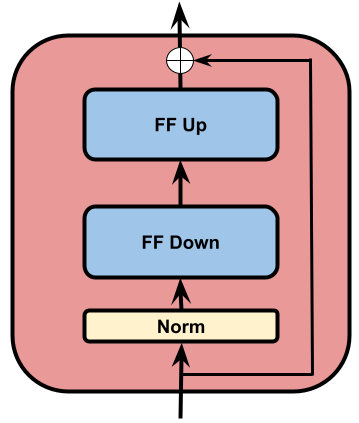
\includegraphics[scale=0.3]{imgs/Adapter_alone.png}
    \caption{Residual Adapter architecture}
    \label{fig:Adapter_architecture}
    \end{center}
    \end{figure*}

    
Adapters were initially introduced in the \ac{NLP} field to efficiently adapt large models, such as Transformers, using a minimal amount of parameters for text classification \cite{houlsby}. As an alternative to full model fine-tuning, Adapter-transfer involves training an extra small number of task-specific parameters while keeping the original model frozen. To this end Adapters are plugged at each Transformer layer level after the \ac{MHA} and \ac{FFN} modules. This setup is often referred to as the \textit{Houlsby} configuration. Subsequently, Pfeiffer \textit{et al.} \cite{pfeiffer} demonstrated that Adapters placed only after the \ac{FFN} modules were sufficient for achieving efficient performances, referred to as the \textit{Pfeiffer} configuration. Typically, Adapters use a bottleneck architecture, consisting of a normalisation layer followed by a projection-down linear layer with a non-linear activation, projecting the input into a $d_{hidden}$ dimension. Subsequently, a projection-up linear layer brings back to dimension $d_{model}$. Finally, a residual connection is applied by summing the input of the Adapter with its output. The overall structure is illustrated in Figure \ref{fig:Adapter_architecture}. Research suggests that the hidden dimension, between the down and up projection, may not always benefit from a bottleneck structure, where $d_{hidden} < d_{model}$, and the optimal design may vary depending on the downstream task \cite{houlsby}. In some tasks, a hidden dimension larger than the model size itself, in other words $d_{hidden} > d_{model}$, has been proven more effective \cite{fan2022draft}.

%Some of the main advantages of Adapters are their parameter efficiency and modularity. This efficiency is particularly interesting when working with large pre-trained models, while modularity is valuable when a large number of tasks need to be trained.
Mathematically, the structure of an Adapter can be expressed as follows:

\begin{equation}
    adapter(x) = x + (W_{up}(f(W_{down}g(x)+b_{down})))+ b_{up})
\end{equation}
Where $W_{down}$ and $W_{up}$ denote the weights of the projection-down and projection-up linear layers with respective dimensions of $\mathbb{R}^{d_{model} \times d_{hidden}}$ and $\mathbb{R}^{d_{hidden} \times d_{model}}$, and $b_{down}$ and $b_{up}$ represent the corresponding biases. The function $f(\cdot)$ is a non-linear activation, while $g(\cdot)$ is a layer normalisation or identity function. Finally, $x$ corresponds to the input given to the Adapter.

In terms of computation, Adapters offer the advantage of faster training, given that they update fewer parameters compared to fully fine-tuning models. Nevertheless, there might be a slight processing delay during inference due to the introduction of extra parameters by the Adapters; however, this difference is generally minimal and can be well-managed \cite{ruckle2020adapterdrop}.

% Adapter ASR
Recently, a rising interest has been observed in Adapter-transfer for \ac{ASR} tasks \cite{cappellazzo2023parameter,chen2023efficient,10095837}, particularly owing to its modular nature, which has proven advantageous in the context of multi-lingual \ac{ASR} \cite{kannan2019large, hou2021exploiting, kulkarni2023adapting}. In these studies, distinct Adapters were trained for each language, contributing to enhanced performance compared to a monolingual model and mitigating certain challenges associated with \ac{TL}, such as overfitting. This modular approach provides a tailored solution, as each Adapter designed for a specific language can effectively capture the diverse acoustic characteristics unique to that language.

Moreover, researchers have explored the use of Adapters in the context of \ac{SSL}. Typically, in \ac{SSL}, larger models are employed to capture a diverse range of information from speech, applicable across a broad spectrum of tasks \cite{thomas2022efficient, fan2022draft}. However, the computational cost and scalability to adapt these models for multiple tasks can be challenging. Notably, once the model is fine-tuned for a specific task, the entire model is fixed for that task, and re-loading and re-training the base model are necessary for transferring to a different task. Therefore, the use of Adapters has proven effective in addressing these challenges by providing a modular and parameter-efficient task-specific adaptation.

%Additionally, the effectiveness of Adapters has been extended by addressing challenges related to low-resource and atypical speech recognition scenarios, as investigated by Tomanek et al. \cite{tomanek2021residual}. This underscores the adaptability and robustness of Adapters, particularly in scenarios where data may be limited or exhibit unconventional characteristics.

Finally, the effectiveness of Adapters has also been demonstrated in addressing challenges related to low-resource and atypical speech recognition scenarios \cite{tomanek2021residual}. This underscores the adaptability and robustness of Adapters, particularly in scenarios where data may be limited or exhibit unconventional characteristics. 
%In such scenarios, similarly to children's speech, there is limited availability of labelled data and atypical speech characteristics. As a result, Adapters provide a valuable solution by efficiently adapting large pre-trained models to these challenging tasks. 

% Adapter children
However, the application of Adapters in the context of children's \ac{ASR} has received limited attention, with only one notable study \cite{fan2022draft}. In this study, the authors introduced a novel approach that involved integrating and training Adapters within \ac{SSL} setting, followed by fine-tuning the entire model, including the Adapter weights,  to enhance the modelling of children's speech. This represents a pioneering effort to leverage Adapters for adapting large-scale models to the unique characteristics of children's speech. Nevertheless, it is crucial to note that in this work, the authors updated the entire model along with the Adapter, compromising the parameter efficiency associated with Adapter-transfer. This highlights the need for a more focused investigation into Adapters as a \ac{PETL} method for children's \ac{ASR}. 

\section{Investigating Adapters for Children's ASR}

\begin{figure*}[t]
    \begin{center}
    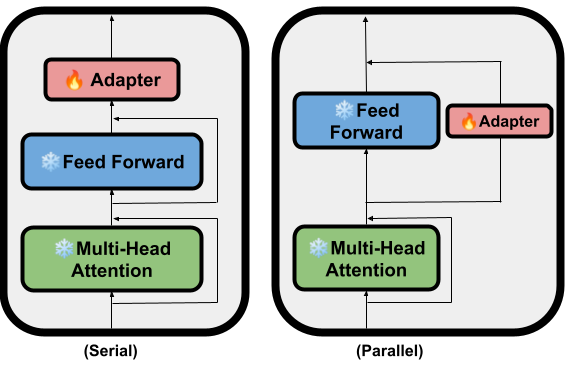
\includegraphics[scale=0.4]{imgs/Adapter_Transformer.png}
    \caption{Transformer block with various residual adapter configurations (Normalisation layers are not shown in this picture for clarity). The fire icon denotes trainable components, whereas the snow icon indicates frozen components.
    }
    \label{fig:transformer_config}
    \end{center}
\end{figure*}
\begin{figure*}[t]
    \begin{center}
    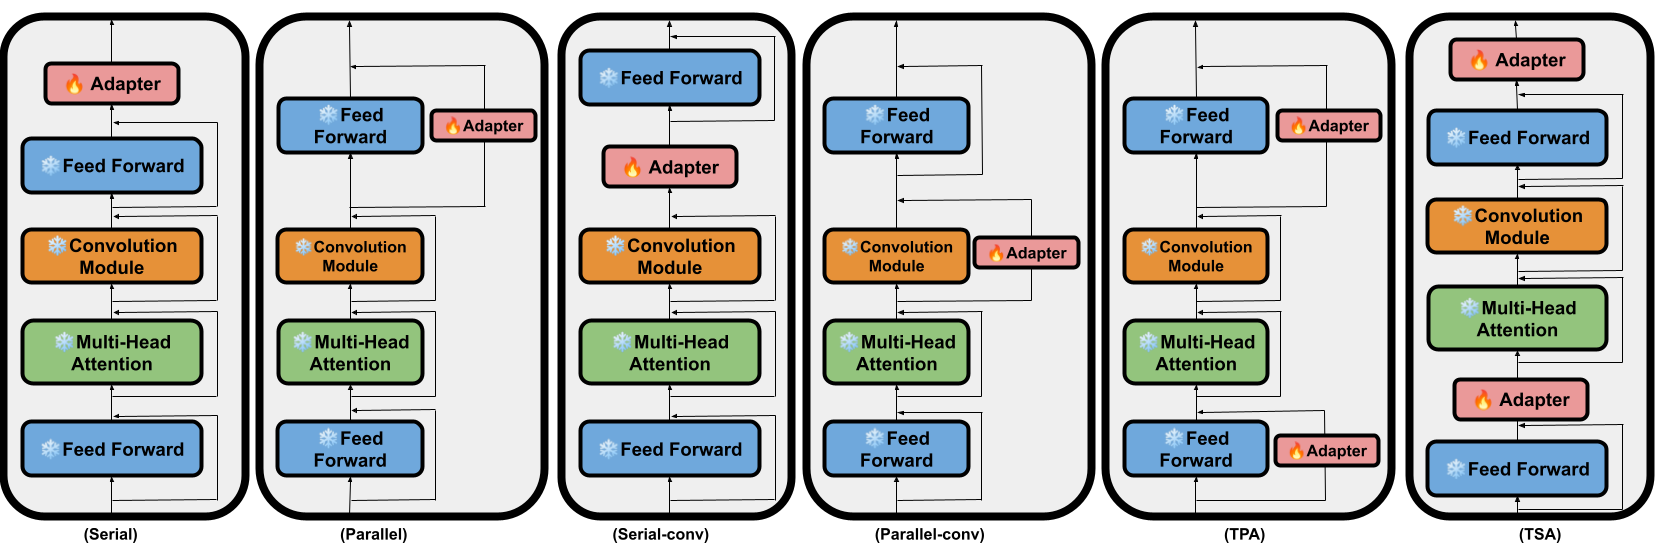
\includegraphics[scale=0.27]{imgs/Adapter_conformer.png}
    \caption{Conformer block with various residual Adapter configurations  (Normalisation layers are not shown in this picture for clarity). The fire icon denotes trainable components, whereas the snow icon indicates frozen components.
    }
    \label{fig:conformer_config}
    \end{center}
\end{figure*}

In this section, we delve into the application of Adapter-transfer as \ac{PETL} for both Transformer and Conformer architectures in the domain of children's \ac{ASR}. Building upon the insights gained from our partial fine-tuning approach in Chapter \ref{chap:4}, we identified \ac{FFN} modules as the most relevant components for fine-tuning in a Transformer-based model. Consequently, we choose to use Adapters for modifying the output of these \ac{FFN} modules. Additionally, given our results that underscored the significance of fine-tuning the Encoder, our primary focus will be on exploring the application of Adapters within the Encoder. For the Transformer architecture, we explore two methods of integrating Adapter modules into the model: \textit{parallel} and \textit{serial} placement with each \ac{FFN} component. These two configurations were used in prior work \cite{he2022towards} and are depicted in Figure \ref{fig:transformer_config}.

In the case of the Conformer architecture, we explore six distinct Adapter configurations, as illustrated in Figure \ref{fig:conformer_config}. The initial two configurations mirror our Transformer investigation, involving both \textit{parallel} and \textit{serial} placements, either after or in parallel with the second \ac{FFN} module \cite{chen2023efficient}. Additionally, we assess a configuration that introduces an Adapter following the convolution module, denoted as the \textit{serial-conv} setup. We evaluate this configuration as it was used in some prior work \cite{10095837}. Notably, although the \ac{FFN} component has been identified as the most crucial for fine-tuning, promising results with our partial fine-tuning have been observed by fine-tuning the convolution modules only. Furthermore, Chen \textit{et al.} \cite{chen2023efficient} introduces two variants of the parallel setup: \textit{parallel-conv} where the Adapter operates in parallel with the convolution module, and the \textit{\ac{TPA}} configuration where two Adapters are placed in parallel with both \ac{FFN} modules in each Conformer layer. 
To comprehensively explore all feasible configurations, we introduce a novel configuration, the \textit{\ac{TSA}}, where two Adapters are sequentially positioned after both \ac{FFN} components in the different Conformer layers. 
This comprehensive exploration of Adapter configurations within both architectures aims to discern the most effective adaptation strategies for children's speech in the context of \ac{ASR}. 


Mathematically, in serial configurations, the Adapter input is provided by the preceding component denoted as $P$, which can be either \ac{FFN} or convolution module, depending on the specific configuration. The output of the Adapter is then determined by the following process:

\begin{equation}
    output =  Adapter(P(x))
\end{equation}

where $x$ represents the input of component $P$.

In parallel configurations, the process varies slightly. In this scenario, the Adapter's input is the same as $P$, and the Adapter's output is combined with the output of component $P$ as follows:

\begin{equation}
    output = x + 0.5 \cdot P(x) + (Adapter(x) - x)
\end{equation}

Furthermore, we consider three distinct configurations where Adapters are integrated into the Decoder. It is important to note that in the Conformer architecture, the Decoder consist of regular Transformer layers. Consequently, we assess both the \textit{Serial} and \textit{Parallel} Adapter setups. Additionally, we examine the combination of the most effective Encoder and Decoder Adapter configurations. To the best of our knowledge, there is no prior research that formally investigates the influence of Adapters within an \ac{ASR} Decoder. 

%Moreover, we consider three distinct configurations where Adapters are placed in the Decoder. It is important to note that in the Conformer architecture, the Decoder is a regular Transformer. Therefore, we evaluate the \textit{Serial} and \textit{Parallel} setups. Subsequently, we investigate the combination of the most effective Encoder Adapter configuration with both Decoder configurations. To the best of our knowledge, there is no prior research that formally investigates the influence of Adapters within an \ac{ASR} Decoder. 

Finally, motivated by the observed strong correlation between children's speech variability and age \cite{TFchildren}, we explore the possibility of training specialised Adapters. However, considering the individual growth speed of each child may not align with a predefined age, using age groups directly may not effectively capture children with similar acoustic characteristics. Additionally, in many children's speech datasets, age information is often not provided. To address this, we propose to partition the dataset into groups of speakers with similar acoustic characteristics based on unsupervised clustering of speaker embeddings.
In practice, we apply a k-means clustering algorithm on the x-vector representation \cite{snyder2018x} of all training utterances. Subsequently, distinct Adapters are trained for each speaker cluster separately. During the testing phase, the closest cluster of the group of speakers is determined for each test utterance, and the corresponding Adapters specific to that group are employed for decoding.
The primary objective of these experiments is to investigate whether Adapters trained on comparable speech characteristics yield improvements over a general Adapter on the entire training set. %Indeed, children's speech is inherently atypical and displays a significant degree of variability, making it imperative to assess the efficacy of existing methods. In prior work, different configurations were employed resulting in a lack of standardised evaluation.

\section{Implementation details}

For all experiments, we used the same pre-trained Transformer and Conformer models described in Section \ref{section:TransformerConformerDetails}. The architecture of each Adapter comprises an initial linear layer projecting to dimension 512 with a \ac{ReLU} activation, followed by another linear layer projecting to dimension 512 with a residual connection from the Adapter input. In the initialisation process for all Adapters, $W_{down}$ was set to all zeros, and $W_{up}$, $b_{down}$, $b_{up}$ were initialised using Xavier initialisation \cite{glorot2010understanding}.

The decision to use a hidden dimension size ($d_{hidden}$) equal to $d_{model}$ instead of employing a bottleneck was influenced by prior research on hidden dimension size. Previous studies consistently demonstrated that larger dimensions tend to result in improved performance scores \cite{chen2023efficient}. All models underwent training of 30 epochs, with a learning rate of $8 \times 10^{-4}$ for training the Adapters and $8 \times 10^{-5}$ for fine-tuning the entire model. In the clustering experiments, we applied the k-means clustering algorithm to the speaker embeddings of each utterance. The speaker embeddings were extracted using a publicly pre-trained ECAPA-TDNN model, trained on adult speech\footnote{https://huggingface.co/speechbrain/spkrec-ecapa-voxceleb}.

For training, we use the My Science Tutor (MyST) Children Speech Corpus, as children dataset. The Myst dataset is the same as it was employed in prior experiments conducted on this dataset within the context of this thesis, as detailed in Table \ref{tab:statistics_myst}. For a more comprehensive understanding of the MyST corpora, additional details are provided in Section \ref{section:children_corpora}.


\section{Results}
\label{sec:results_adapters}

\subsection{Adapter Configurations}
\begin{table}[h]
\begin{center}    
\begin{tabular}{ccc}
\hline
 Method & WER $\downarrow$     & Trained params    \\ \hline \hline
\multicolumn{3}{c}{\textbf{Transformer}} \\ \hline
\multicolumn{1}{l}{\textit{Frozen}} & 25.04   & - \\
\multicolumn{1}{l}{\textit{Full fine-tuning}} & 12.99 & 71.5M \\ \hline
\multicolumn{1}{l}{Serial}  &   12.78 & 6.3M  \\ 
\multicolumn{1}{l}{Parallel}  &     \textbf{12.62} & 6.3M  \\ \hline\hline
\multicolumn{3}{c}{\textbf{Conformer}} \\ \hline
\multicolumn{1}{l}{\textit{Frozen}} & 21.75   & - \\ 
\multicolumn{1}{l}{\textit{Full fine-tuning}} & 12.28 & 109.1M \\ \hline
\multicolumn{1}{l}{Serial}  &   11.76 & 6.3M  \\ %11.84 
\multicolumn{1}{l}{Serial-Conv} & 11.78    & 6.3M  \\
\multicolumn{1}{l}{Parallel}    & 11.72 & 6.3M  \\ % 11.88 
\multicolumn{1}{l}{Parallel-conv} & 11.79      & 6.3M  \\ %\hline
\multicolumn{1}{l}{TPA} & \textbf{11.58}     & 12.6M  \\ %11.85
\multicolumn{1}{l}{TSA} & 11.75     & 12.6M  \\ \hline %11.72
\multicolumn{1}{l}{Serial (Decoder)} & 18.09     & 3.2M  \\ 
\multicolumn{1}{l}{Parallel (Decoder)} &17.76     & 3.2M  \\ \hline
%\multicolumn{1}{l}{TPA + Serial (Decoder)} & 00.00(T)\%     & 15.8M  \\
%\multicolumn{1}{l}{TPA + Serial (Decoder)} & 11.68\%     & 15.8M  \\ 
\multicolumn{1}{l}{TPA + Parallel (Decoder)} & \textbf{11.47}     & 15.8M  \\ \hline

\end{tabular}
\end{center}
\caption{Results of the different Adapters configurations in both Transformer and Conformer. WER expressed in terms of percentage.}
\label{tab:res_config}
\end{table}

In this section, we present a comprehensive evaluation of the different Adapter configurations applied to both Transformer and Conformer models. These results are presented in Table \ref{tab:res_config}. First, we assess the Transformer model when no fine-tuning was applied (\textit{Frozen}), resulting in a \ac{WER} of 25.04\%. Conversely, \textit{Full Fine-Tuning} involved complete fine-tuning of the entire model, working as our baseline system, reducing the \ac{WER} significantly to 12.99\%, with the use of 71.5 million trainable parameters.
Turning to the Adapter setups, we investigate the \textit{Serial} and \textit{Parallel} configurations, both using 6.3 million trainable parameters. The \textit{Parallel} emerged as the best configuration, achieving the lowest \ac{WER} of 12.62\% compared to 12.78\% for the \textit{Serial}. These results underscore the effectiveness of Adapter configurations within the Transformer architecture, as they both perform slightly better than the full-finetuning baseline.

Next, we investigated the Conformer architecture, we once again explored \textit{Frozen} and \textit{Full Fine-Tuning}. The \textit{Frozen} pre-trained model yielded a \ac{WER} of 21.75\%, while the full fine-tuning, in a similar way as the Transformer, led to enhanced performance, with \ac{WER} of 12.28\% using a total of 109.1 million trainable parameters. Within the set of Adapter configurations, \textit{Serial} achieved a \ac{WER} of 11.76\%, while \textit{Parallel} demonstrated slightly better performance with a \ac{WER} of 11.72\%. These results confirm that \textit{Parallel} Adapters were more effective in improving \ac{WER} in both Transformer and Conformer models. When Adapters are placed after the convolution layer, with the \textit{Serial-conv} and \textit{Parallel-conv} configuration, both slightly under-perform compared to Adapters placed after the second \ac{FFN} component with respective scores of 11.78\% and 11.79\%. Finally, we evaluated the \textit{\ac{TPA}}and \textit{\ac{TSA}} configurations. The \textit{\ac{TPA}} configuration emerged as the most promising, with a remarkable \ac{WER} of 11.58\% using 12.6 million trainable parameters, while \textit{\ac{TSA}} achieved a \ac{WER} of 11.75\%, which is slightly under-performing compared to the \textit{\ac{TPA}} configuration.

In addition, we evaluated the use of Adapters in the Decoder. As the Decoder of the Conformer architecture is a regular Transformer, we only evaluate the \textit{Serial} and \textit{Parallel} setup, which respectively reached 18.09\%  and 17.76\% \ac{WER} with 3.2 million parameters. These results showed that Adapters are more relevant when plugged into the Encoder which is in line with findings from Chapter \ref{chap:4}. Finally, combining \textit{\ac{TPA}} in the Encoder layers with \textit{Parallel} Adapters in the Decoder outperforms Adapters in the Encoder only, with 11.47\% \ac{WER}. Consequently, this configuration stands as the most effective configuration for our children's speech dataset. 

%statistical tests
We performed statistical tests (Matched Pairs Sentence-Segment Word Error) across all Adapter setups in comparison to the full fine-tuning configuration using SCTK, the NIST Scoring Toolkit \cite{SCTK_nist}. 
The results reveal that, in all scenarios, the \textit{p}-value is less than or equal to 0.001. This observation denotes statistical significance, indicating evidence against the null hypothesis. 

These results collectively illustrate the versatility and effectiveness of different Adapter configurations within the Transformer and  Conformer model for the children's \ac{ASR} task. \textit{\ac{TPA}} Adapters in the Encoder combined with \textit{Parallel} Adapters in the Decoder showcased outstanding performance, highlighting their potential as a fine-tuning replacement in large model children \ac{ASR} scenarios.

\subsection{Effect of the Adapters hidden dimension}
\label{sec:hidden_size_adapter}
\begin{figure}[h]
    \begin{center}
    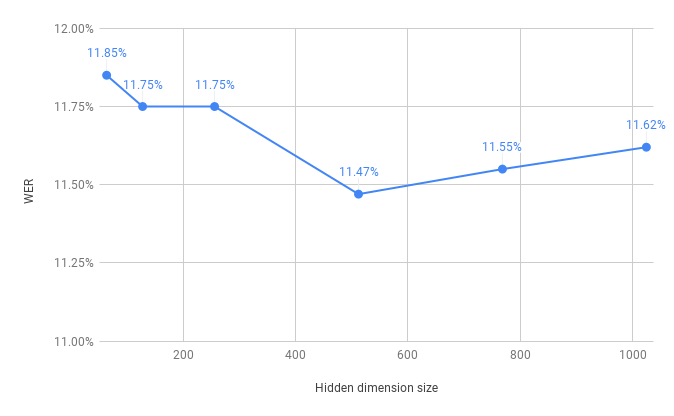
\includegraphics[scale=0.5]{imgs/HiddenDimEXP.png}
    \caption{Experimental Adapter transfer using different hidden dimension sizes within the Conformer architecture.}
    \label{fig:HiddenDim}    
\end{center}
    
\end{figure}

In this section, our objective is to assess the influence of different hidden dimension values for the Adapter ($d_{hidden}$) on the model's performance. In our previous experiments, we maintained a fixed hidden dimension, where $d_{model} = d_{hidden} = 512$. Now, we aim to explore various hidden dimension values within the Conformer architecture, focusing on the \textit{\ac{TPA}} in the Encoder-only configuration. This investigation aims to assess how variations in the hidden dimension may impact the performance of the Adapter transfer, offering valuable insights into the parameter tuning process for Adapter modules.

In Figure \ref{fig:HiddenDim}, the relative \ac{WER} delta compared to the full model fine-tuning performances of the Adapter transfer are presented in relation to the hidden dimension size ($d_{hidden}$), and therefore the relative amount of parameters compared to the entire model. Notably, a trade-off is observed, emphasising the importance of choosing an optimal hidden dimension size. Configurations with dimensions that are either too small or too large result in a degradation of overall performance. The best-performing configuration aligns with the choices made in all previous experiments, with $d_{hidden} = d_{model} = 512$. We hypothesise that the parallel Adapter functions as an extension of the key-value memory of the \ac{FFN}. Opting for an extremely large hidden dimension makes training more complex due to a large number of parameters, while an excessively small size drastically limits the potential information learned from the Adapters. 

\subsection{Unsupervised clustering for grouped-speaker Adapters}
\label{sec:clustering_emb}
\begin{table}[h]
    \begin{center}    
    \begin{tabular}{cc}
    \hline
      \# of clusters & Average WER $\downarrow$    \\ \hline
    \multicolumn{1}{c}{1} & 11.58  \\% OR 11.70%  If we consider 40 epochs instead of 30 here
    \multicolumn{1}{c}{2} & \textbf{11.50}  \\
    \multicolumn{1}{c}{3} & 11.57  \\
    \multicolumn{1}{c}{4} & 11.51  \\ \hline 
    \end{tabular}
    \end{center}
    \caption{Results of the unsupervised clustered Adapters approach. WER expressed in terms of percentage.}
    \label{tab:res_clusters}
    \end{table}


In this section, we present the outcomes of our clustering approach summarised in Table \ref{tab:res_clusters}. The investigation focuses on the influence of varying the number of clusters on the \ac{ASR} scores, ranging from 1 to 4 clusters, using the \textit{\ac{TPA}} configuration in an Encoder-only setup within the Conformer model.

Initially, when the data remained unclustered, corresponding to one cluster, the \ac{ASR} system exhibited a \ac{WER} of 11.58\%. Notably, the two-cluster configuration outperformed the other setups, achieving superior performance with a \ac{WER} of 11.50\%. This result suggests that partitioning the data into two distinct clusters allows the different Adapters to more effectively capture underlying patterns intricately linked to their respective clusters, consequently enhancing the recognition scores.

Furthermore, we explored the impact of increasing the number of clusters to three and four, revealing only marginal differences in performance. Specifically, the three-cluster configuration yielded a \ac{WER} of 11.57\%, and the four-cluster configuration resulted in a \ac{WER} of 11.51\%. These findings underscore the role of data clustering in children's \ac{ASR} systems by grouping shared speaker characteristics into different clusters.


In summary, our investigation emphasises the role of data clustering in the context of children's \ac{ASR} systems. Specifically, for the Myst dataset, optimal performance was attained with a two-cluster configuration, suggesting that this approach facilitates the effective capturing of cluster-specific patterns by the Adapters. The marginal performance differences observed with three and four clusters suggest a potential saturation point, indicating that further partitioning may yield diminishing returns in terms of \ac{ASR} performance improvement for this specific dataset.

It is noteworthy that, in this experiment, the amount of available training data for Adapters varies due to the clustering process. A more comprehensive exploration of the impact of training hours on Adapters will be presented in Section \ref{sec:hours_PETL}. This forthcoming analysis will offer a detailed understanding of how different training amount of data influence the performance of Adapters in diverse conditions, shedding light on their adaptability and effectiveness across various scenarios.

Additionally, considering the relatively narrow age range of the Myst corpus, encompassing children from the third to fifth grade, future work could explore the applicability of this approach on children datasets with a more extensive age range. This extension would contribute valuable insights into the generalisation and robustness of the clustering-based Adapter approach across diverse age groups within the realm of children's \ac{ASR}.

    
\section{Summary and discussion}
% Summary
In this chapter, we investigated the viability of Adapter-transfer in the context of children's \ac{ASR}. Addressing the research question, \textit{Does parameter efficient transfer improve children \ac{ASR} compared to full model fine-tuning?} our investigation yielded an affirmative response. Our study showcased the effectiveness of adapting the model using Adapter modules, resulting in improved \ac{WER} performances compared to full-model fine-tuning. Notably, this was achieved while utilising only approximately 10\% of the parameters required in the traditional transfer learning of the entire model, underscoring the parameter efficiency of Adapter-transfer.
 
Among the various configurations explored in this chapter, the ``parallel" Adapter and its extension, the ``\ac{TPA})" emerged as the most effective choices for the Transformer and Conformer architectures, respectively. The ``parallel" Adapter, in particular, demonstrated its efficacy as it extends the key-value memory that represents the \ac{FFN} modules \cite{geva2020transformer}, showcasing its potential to capture essential information specific to children in a more parameter-efficient manner.

Building on these findings, we proposed the integration of unsupervised clustering on the speaker embeddings extracted from different utterances into the Adapter-transfer procedure. This strategic clustering aimed to facilitate the training of specific Adapters for each cluster, offering a more personalised adaptation without relying on detailed metadata about the speaker, such as their age. Our results illustrated that leveraging these clusters could further enhance overall performances, opening avenues for the application of Adapters for better personalised \ac{ASR} systems.


% Discussion
% Mention that this opens the way for other uses, such as reducing the domain mismatch
The successful implementation of Adapter transfer in the domain of children's speech presents promising opportunities for advancing children's \ac{ASR}. Our findings indicate that Adapters serve as effective tools for bridging the gap between a source and a target domain while retaining the valuable knowledge encapsulated in pre-trained models. This promising outcome lays the foundation for further exploration. In the upcoming chapter, we will extend our research by investigating the application of Adapters in the domain of \ac{TTS} data augmentation. This extension aims to leverage the capabilities of Adapters to reduce the disparity between real and synthetic children's speech.

% Also mention that we will investigate other PETL approaches
Moreover, in addition to the Adapter module introduced in this chapter, it is noteworthy to mention that various \ac{PETL} alternatives exist in the literature, demonstrating their effectiveness in tasks beyond children's \ac{ASR}, such as \ac{NLP} tasks demonstrating in some scenario better accuracy and parameter efficiency. Therefore, in the next chapter, we will extend our exploration of \ac{PETL} modules, evaluating their applicability and performance in the specific context of children's \ac{ASR}. Additionally, we will delve into the development of new \ac{PETL} approaches, aiming to strike a better balance between parameter efficiency and accuracy. 



% If Printing on DOUBLE SIDED pages, the second page should be white.
% Otherwise, comment the following command:
\cleardoublepage{}
%
%Chapter 6
%% #############################################################################
% This is Chapter 6
% !TEX root = ../main.tex
% #############################################################################
% Change the Name of the Chapter i the following line
\fancychapter{Integration of synthetic speech for data augmentation}
\label{chap:6}
\cleardoublepage

\section{Introduction}
% Challenge in children speech
As mentioned in Chapter \ref{chap:Chapter2}, the ongoing advancements in deep learning, coupled with the availability of extensive training datasets, have undeniably improved the ASR performances. However, despite these remarkable advancements, the recognition of children's speech remains a domain where performance lags behind that achieved for adult speech. Children's speech introduces distinct challenges owing to its inherent variability influenced by age, linguistic development, and articulatory differences. Therefore, there is a growing need acquiring a sufficiently diverse and extensive dataset for training children's ASR systems. 

However, practical constraints, including ethical considerations, privacy concerns, the high cost of data collection, the challenges posed by children's limited attention span and inconsistent adherence to prompts during reading tasks, hinder the creation of such datasets. In an effort to address this performance gap, researchers in \cite{asr-google} leveraged an in-house sizable dataset of children's speech, comparable in scale to an adult corpus, to train an ASR model. The outcomes showcased state-of-the-art performances, emphasising the potential of ASR systems to effectively learn from diverse and variable children's speech data when provided with a substantial amount of training data.

As an answer to the challenges of collecting real childen's speech data, an alternative strategy emerged, involving the generation of synthetic datasets using a Text-to-Speech (TTS) model. TTS offers a solution to bypass to the challenges associated with collecting and annotating real children's speech data. While some studies have explored the application of TTS for ASR, either through direct use of synthetic speech for training or as a form of data augmentation \cite{laptev2020you,fazel21_interspeech}, synthesising children's speech introduces a unique set of challenges. The inherent substandard and imprecise pronunciation in children's speech \cite{wang2021towards} poses an hurdle, raising concerns that the direct use of synthetic data may lead to a decrease in performance \cite{wang2021towards, hu2022synt++}.

% Our Approach
In this chapter, we introduce a novel technique known as ``Double-Way Adapter Tuning", or DWAT, to enhance ASR models specifically for children's speech, even in scenarios where imperfect data are employed as augmentation. Our approach involves the integration of additional Adapter modules into the existing ASR model during the fine-tuning process. As demonstrated in the preceding chapter \ref{chap:5}, Adapters have proven to be efficient in transferring knowledge for children's speech, thereby serving as a parameter-efficient means of knowledge transfer. But also as a novel way to reduce the gap between a source and target domain while preserving the source knowledge in the pre-trained model.
Building upon the efficiency of Adapters in the realm of children's speech, we hypothesise that these Adapters can be used to mitigate the domain mismatch between real and synthetic data. We accomplish this through a two-step training procedure in a similar way as the methodology proposed in \cite{fan2022draft}.

In the initial step, the Adapters are exclusively trained using synthetic data, while the pre-trained model remains frozen. This phase enables the Adapters to specialise in handling the nuances introduced by synthetic data. Subsequently, in the second step, we perform fine-tuning, involving both the trained Adapters and the entire model weights. During this fine-tuning process, a combination of synthetic and real data is given to the model. Notably, our approach introduces a crucial distinction between synthetic and real data throughout the fine-tuning process. Synthetic data traverses the Adapter layers, allowing the synthetic characteristics to be handle by the Adapters while  still contribute to the full model tunning, while real data bypasses these Adapters. We hypothesise that this meticulous differentiation could enables the effective use of imperfect synthetic data, ultimately leading to an enhancement in ASR performances.

In this chapter, our objective is to address the research questions: \textit{Is it possible to use children's synthetic speech to extend the amount of children's data? How can we control the quality and speakers’ variability?}

%In this chapter, we introduce a novel technique called "Adapter double-way fine-tuning" to enhance ASR models for children, even when using imperfect data augmentation. Our approach involves adding additional adapter layers to the existing ASR model during fine-tuning, similar to \cite{fan2022draft}. These adapter layers are customised to address the domain mismatch between real and synthetic data. We achieve this through a two-step training procedure. In the first step, the adapter layers are trained exclusively using synthetic data while keeping the pre-trained model frozen. In the second step, we fine-tune both the trained adapters and the entire model using a combination of synthetic and real data. Crucially, our approach differentiates between synthetic and real data during fine-tuning. Synthetic data passes through the adapter layers, while real data bypasses them. This approach enables the effective use of imperfect synthetic data to enhance ASR performance for children.


%\section{Related work}
\section{Enhancing ASR Performance through TTS Data Augmentation}
%TTS data augmentation
The progression of TTS systems, achieving human-like quality, presents a valuable avenue for effective TTS-based data augmentation in ASR. This approach, as exemplified in studies such as \cite{laptev2020you}, involves the generation of synthetic speech from text using TTS models. The synthetic speech is then combined with real speech during the training process, leading to notable performance enhancements. Importantly, this approach is not limited to well-resourced tasks and has demonstrated success even in low-resource scenarios, as illustrated in \cite{casanova2022asr}. However, despite its efficacy, TTS-based data augmentation offers only modest improvements, primarily owing to the persistent challenge of domain mismatch between synthetic and real speech, indeed, even with human-like quality, some generated utterances suffer artefacs or wrong modelisation. The inherent differences between the characteristics of synthetic and real speech limit the extent to which the benefits of TTS augmentation as ASR data augmentation. 
%The advancement of TTS systems, achieving human-like quality, enables effective TTS-based data augmentation in ASR. This approach, as shown in studies like \cite{ laptev2020you}, involves generating synthetic speech from text using TTS models, then combining it with real speech for training, resulting in performance enhancements. Notably, this approach is not limited to well-resourced tasks and has succeeded in low-resource scenarios, as demonstrated in \cite{casanova2022asr}. Nevertheless, TTS data augmentation offers only modest improvement due to the domain mismatch between synthetic and real speech. 
% To this end, \cite{9688218} proposed to use discrete representations based on VQ-wav2vec, allowing to mitigate the mismatch with real data and reducing speaker dependency.


In order to mitigate the mismatch with real data and to reduce speaker dependency,  the use of discrete intermediate representations both shared by the TTS and ASR systems instead of Mel-scale filterbanks, obtained with a VQ-wav2vec, has been proposed in \cite{9688218}. This approach has demonstrated promising results. However, it is essential to note that implementing such a strategy necessitates training both the ASR and TTS systems from scratch. This requirement may pose challenges, particularly in the context of low-resource ASR scenarios

% Children data selection
An alternative approach to address the domain mismatch between synthetic and real speech rely on data selection techniques, as proposed by \cite{wang2021towards}.  This approach focuses on selectively choosing high-quality synthetic speech data to mitigate the challenges associated with imperfect data augmentation. The data selection process ensures that only the most reliable and accurate synthetic speech samples are incorporated during the augmentation process. One advantageous aspect of this work is that it does not necessitate more complex training for the TTS or ASR system. Instead, it operates as an off-the-shelf selection on top of the TTS system. This characteristic underscores the practicality and ease of it integration into existing TTS systems.
In \cite{wang2021towards}, they demonstrated the effectiveness of employing i-vector speaker-embedding cosine similarity between reference and generated utterances as a metric for data selection. This metric was compared to other metrics such as error rate, acoustic posterior, and synthetic discriminator. 
%Another approach to mitigate the domain mismatch between synthetic and real speech is through the use of data selection techniques, as suggested by \cite{wang2021towards}. By selectively choosing high-quality synthetic speech data. This data selection process ensures that only the most reliable and accurate synthetic speech samples are used during data augmentation. The results presented in \cite{wang2021towards} demonstrate the effectiveness of employing i-vector speaker-embedding cosine similarity as a metric for data selection, compared to metrics like error rate, acoustic posterior, and synthetic discriminator.

% Synth++
More recently, \cite{hu2022synt++} introduced the Synth++ framework, which employs a similar data selection approach, called rejection sampling. This rejection sampling method relies on the output of a DNN, which is trained on a 5-dimensional features vector derived from a pre-trained ASR model. The goal of this DNN is to discriminate either the data is real or synthetic. To this end, the 5-dimensional features vector for each utterances encompass cross-entropy loss, CTC loss, WER, lengths of tokens in the predicted text and the length of tokens in the target text. In addition to rejection sampling, Synth++ introduces the use of separate batch normalisation for real and synthetic data. During the training process, when synthetic data is fed into the model, it undergoes distinct normalisation layers. The incorporation of this separated normalisation has been demonstrated to significantly reduce the mismatch between real and synthetic data during training, leading to notable improvements in WER scores.

% In Synth++ \cite{hu2022synt++}, an extension to the data selection technique is proposed, by incorporating separate batch normalization statistics for real and synthetic samples. While data selection handles artefacts and over/under-sampling, double batch normalization aims to further bridge the synthetic-real data gap during training. This approach uses rejection sampling based on a DNN's output. Where the DNN is trained on a 5-dimensional features vector derived from a pre-trained ASR model, including cross-entropy loss, CTC loss \cite{First_End2End}, word error rate (WER), lengths of tokens in prediction text, and length of tokens in target text, offering valuable insights into speech quality and characteristics.
% However, we find out that it may not be working. HERE?

\section{Closing the synthetic and real mismatch gap with Adapters}

\begin{figure*}
    \centering
    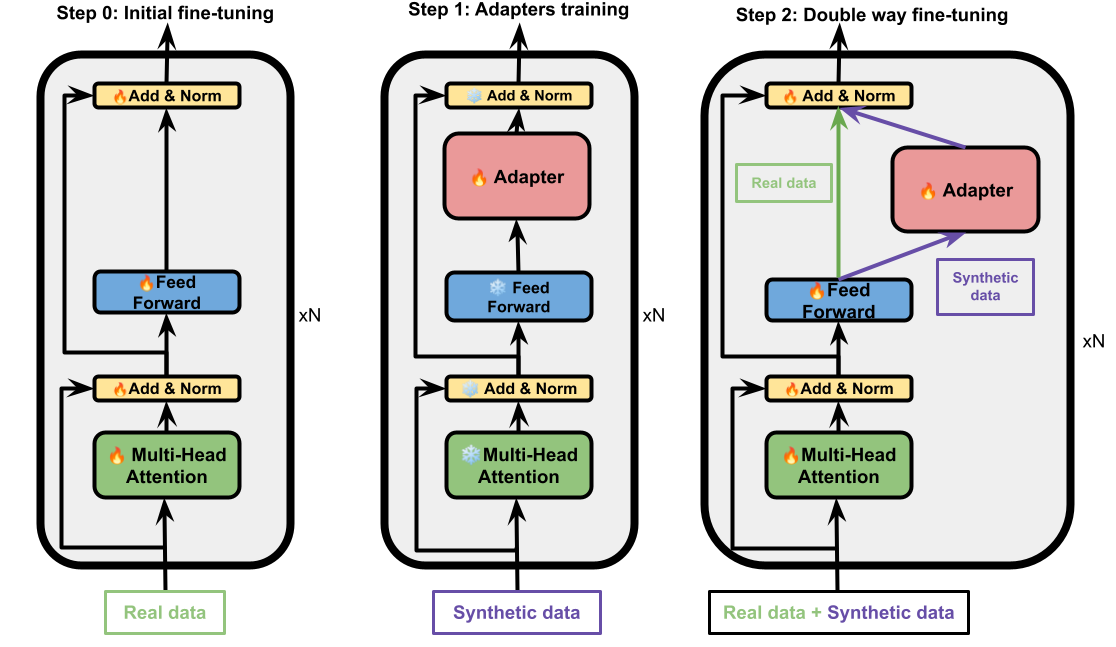
\includegraphics[width=\textwidth]{imgs/TTS_Transformer.png}
    \caption{Overview of ``Double way Adapter fine-tuning"  within th context of an Transformer model}
    \label{fig:overall}
\end{figure*}

The effectiveness of Adapters in the existing literature for both speech and NLP tasks has been well-documented \cite{pfeiffer, philip2020monolingual, mao-etal-2022-unipelt}. Additionally, the positive results detailed in Chapter \ref{chap:5}, where Adapter modules were proven effective for children's ASR, underscore their pivotal role in mitigating the mismatch between a source model and a target task. Proving that Adapters are capable of capturing task-relevant information, while the frozen pre-trained model retains valuable insights about the source task.

In alignment with these findings, \cite{fan2022draft} introduced the Domain Responsible Adaptation and Fine-Tuning framework (Draft) for children's ASR. The authors aimed to reduce the mismatch between adult and children speech data in SSL models by incorporating Adapters and an additional adaptation phase. Leading to improved performances.

Motivated by the successes of the Draft framework and Synth++, our approach integrates Adapter modules as a substitute for the separate normalisation layers present in the Synth++ framework. Furthermore, we incorporate the multiple-step adaptation and the use of Adapters from the Draft framework. Finally, we employed filtered synthetic data, implementing a speaker-embedding cosine similarity metric to retain synthetic utterances that exhibited high-quality generation as pproposed by previous work on data selection for TTS data augmentation. This combination forms a novel strategy to address the domain mismatch in ASR for children's speech, called ``Double-way Adapter tunning" (DWAT). 


Our primary goal is to inject external knowledge of synthetic children's speech into a pre-trained ASR model using Adapters. This approach allows us to preserve the real children's speech knowledge acquired during pre-training while separately modeling the synthetic characteristics within the Adapter modules. Therefore, Adapters serves as a bridge, that can effectively reducing the domain mismatch between real and synthetic speech data during the training of ASR models for children using a combination of real and synthetic data. 

In our DWAT  methodology, as illustrated in Figure \ref{fig:overall}, we introduce two additional steps following the standard ASR model training with children's data (Step 0).
% Step 1
Step 1 involves the standard training of Adapter modules, as explained in the previous chapter. While keeping the pre-trained ASR model parameters fixed, the Adapter weights are trained on the target data, here TTS utterances. These Adapter modules are strategically placed after the transformer layers' Feed-Forward Network (FFN) component. The goal is to learn a projection that aligns synthetic children's speech with real children's speech within each transformer layer. This approach allows the model to retain knowledge about children's speech, while the Adapters aim to capture the synthetic characteristics of the different TTS utterances. This step is crucial, as Adapter modules require this learning process. Without it, the subsequent fine-tuning in Step 2 could be more challenging and less effective.
%Step 1 entails the regular training Adapter modules, as presented in previous chapter. While keeping the pre-trained ASR model parameters fixed the Adpaters weights are being trained. These Adapter modules are placed after the transformer layers' FFN component, aiming to learn a projection that aligns synthetic children's speech with real children's speech within each transformer layers. By doing this, the model will still contains knowledge about children's speech while the Adapters should models the synthetic characteristics of the TTS utterances. This step is crucial as Adapter modules require this learning process. Without it, the subsequent fine-tuning in Step 2 could be more challenging and less effective.
%Step2
In Step 2, we fine-tune both the Adapters trained in Step 1 and the entire pre-trained ASR model using a mix of synthetic and real data. A pivotal aspect of our approach lies in how we handle data flow within the model. Real samples bypass the Adapter modules as they do not need further adjustments, directly passing through the original ASR model components. In contrast, synthetic data goes through the Adapters for necessary modifications to better align with real children's speech characteristics. This differential treatment of data optimises Adapter usage, potentially enhancing the overall performance of the ASR system.
%In Step 2, we fine-tune both the Adapters trained in Step 1 and the pre-trained ASR model using a mix of synthetic and real data. A crucial aspect of our approach is how we handle data flow within the model. Real samples bypass the adapter modules as they do not need further adjustments, directly passing through the original ASR model components. Synthetic data, on the other hand, goes through the Adapter for necessary modifications to align better with real children's speech characteristics. This differential treatment of data optimises adapter usage, potentially improving the ASR system's overall performance.
% Inference
During the inference phase, the Adapter modules become unnecessary and are discarded since the test data only contains real samples and the training is already complete. It is essential to note that Steps 1 and 2 can be iteratively repeated with newly generated synthetic data. However, it's important to highlight that this aspect is not thoroughly investigated in this work and serves as a subject for future research. The potential iterative repetition of these steps could provide insights into the adaptability and generalisation capabilities of the proposed Double-Way Adapter Tuning methodology.
%During inference, the Adapter modules become unnecessary and are discarded because the test data only contains real samples. It is important to mention that Steps 1 and 2 can be iteratively repeated with newly generated synthetic data, although this aspect is not investigated in this paper and is a subject for future research.


%Building on the successes observed with Adapters in the existing literature for speech and NLP tasks \cite{pfeiffer, philip2020monolingual, mao-etal-2022-unipelt}, and the results detailed in Chapter \ref{chap:5}, where Adapter modules were found to be effective for children's ASR, we propose leveraging Adapter modules to bridge the gap between real and synthetic speech data. 

%The motivation of our work is to expend on the achievements of the Draft framework and Synth++. Indeed, our approach use Adapters as a substitute for the double batch normalisation layers present in the Synth++ framework and use the multiple step adaptation with Adapters from Draft.

% Explain adapters
%Adapters were first introduced for natural language processing (NLP) tasks as a simpler alternative to full model fine-tuning \cite{houlsby}. They involve adding a small number of extra parameters to each layer of the transformer model. Unlike full fine-tuning, which modifies the entire model, adapters enable targeted adjustments within specific layers while keeping pre-trained parameters intact. These adapters typically follow a bottleneck architecture with down-projection and up-projection, as seen in Figure \ref{fig:overall}-b. The bottleneck architecture's purpose is to introduce non-linear transformations, enabling Adapters to capture task-specific features and learn task-specific modifications effectively.

%Since their proposal, adapters have demonstrated effectiveness in diverse NLP tasks, including language understanding and neural machine translation \cite{philip2020monolingual}. Additionally, there is a growing interest in applying adapters to automatic speech recognition. For instance, \cite{tomanek2021residual} explored adapters for atypical speech, focusing on pathological and accented speech.
% Draft
%In children's ASR, Adapters are employed within the Draft framework \cite{fan2022draft}. This approach inserts and trains Adapters at each block of a pre-trained self-supervised learning (SSL) model using an SSL loss. Subsequently, the entire model, including the Adapters, undergoes fine-tuning with ASR losses. By combining SSL pre-training, Adapters, and full fine-tuning, this approach uses the advantages of SSL, the adaptability of adapters, and task-specific fine-tuning to enhance the recognition accuracy of ASR systems for children's speech.

%\section{Method}


% Motivation
%Expanding on the achievements of the Draft Framework and Synth++, our approach utilizes Adapters as a substitute for the double batch normalization layer of the Synth++ framework. Our aim is to improve the performance of a pre-trained ASR model through data augmentation using synthetic data. In our methodology, we employed filtered synthetic data, implementing a speaker-embedding cosine similarity metric to retain synthetic utterances that exhibited high-quality generation. Our approach introduces two extra steps following the standard ASR model training (Step 0).%NEW
%Figure \ref{fig:overall}-a provides an overview of our proposed methodology.

% Step 1
%Step 1 entails training Adapter layers while keeping the ASR model parameters fixed. These Adapter layers are placed after the transformer layers' feed-forward component, aiming to learn a projection that aligns synthetic children's speech with real children's speech within the transformer layers. This step is crucial as Adapter layers require this learning process. Without it, the subsequent fine-tuning in Step 2 could be more challenging and less effective.

%Step2
%In Step 2, we fine-tune both the adapters from Step 1 and the pre-trained ASR model using a mix of synthetic and real data. A crucial aspect of our approach is how we handle data flow within the model. Real samples bypass the adapter layers as they don't need further adjustments, directly passing through the original ASR model components. Synthetic data, on the other hand, goes through the adapter layers for necessary modifications to align better with real children's speech characteristics. This differential treatment of data optimises adapter usage, potentially improving the ASR system's overall performance.

% Inference
%During inference, the Adapter layers become unnecessary and are discarded because the test data only contains real samples. It is important to mention that Steps 1 and 2 can be iteratively repeated with newly generated synthetic data, although this aspect is not investigated in this paper and is a subject for future research.
 
% Recap
In summary, our proposed approach use Adapter modules to enhance the performance of a pre-trained ASR model through the incorporation of synthetic data augmentation. This innovative methodology, known as DWAT introduces a two-step process involving the training of Adapter and subsequent fine-tuning with a mix of synthetic and real data in order to bridge the domain gap between real and synthetic children's speech.

%In summary, our approach uses adapter modules to improve the performance of a pre-trained ASR model through the integration of filtered synthetic data augmentation.




\section{Overview of the automatic speech recognition and text-to-speechs systems}
\label{section:SOA}
\subsection{Transformer architecture for ASR}
% Motivation children E2E
%The Transformer architecture, initially developed for tasks like machine translation \cite{Transformer}, was found to be highly effective and widely used in various domains, including computer vision \cite{VIT} and language understanding \cite{Bert}. In speech recognition, it takes acoustic features as input, processes them through an encoder to create high-level representations, and uses these for token prediction in a decoder. Training typically combines a sequence-to-sequence approach with a CTC loss \cite{CTC}.
%Recent studies, such as \cite{sri_end2end}, demonstrate that fine-tuning adult pre-trained Transformer-based models with children's speech data yield better results than traditional HMM-DNN based models, making the Transformer-based and End-to-end models a suitable choice for children's ASR.
In our experiments, we employed the SpeechBrain toolkit \cite{speechbrain} for the ASR component of our system, using a pre-trained Transformer model\footnote{https://huggingface.co/speechbrain/asr-transformer-transformerlm-librispeech}. This model has trained on the LibriSpeech dataset \cite{librispeech} and comprises 12 encoder layers and 6 decoder layers, each with a dimension of 512. It is noteworthy, that is model is different from the ones used in previous Chapters. A mix of sequence-to-sequence and CTC loss where used with respective weight of 0.7 and 0.3. Additionally, we integrated a Transformer language model trained on a 10 million-word transcriptions of Librispeech.

\subsection{Multi-speaker text-to-speech: YourTTS}

\begin{figure}
    \begin{center}
        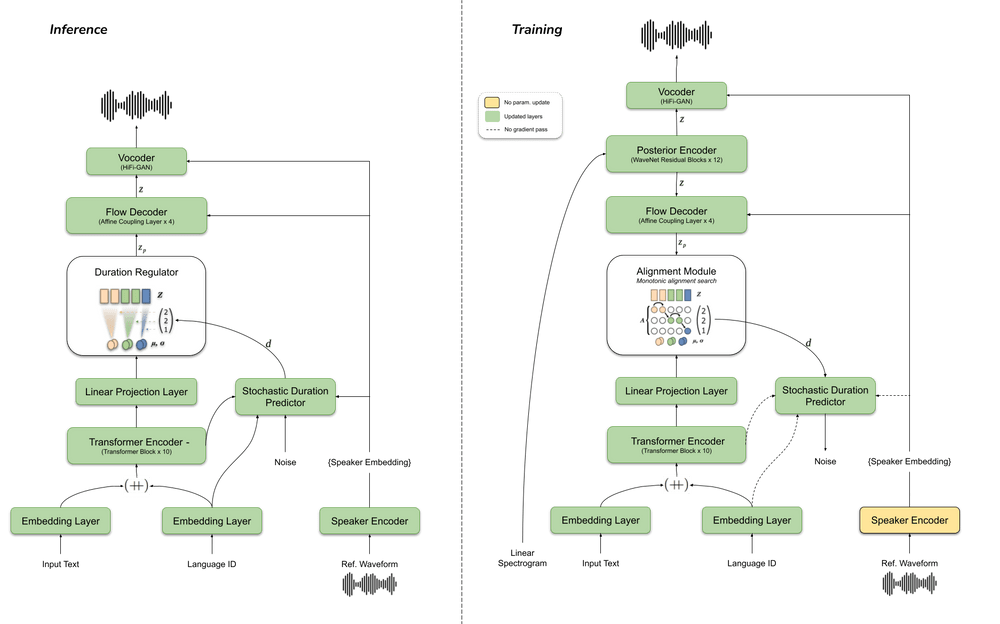
\includegraphics[scale=0.4]{imgs/yourtts.png}
        \caption{Architecture of the YourTTS model taken from \cite{casanova2022yourtts}}
        \label{fig:yourtts}
    \end{center}
\end{figure}

In this work as TTS component, we used the pre-trained YourTTS model\footnote{https://coqui.ai/blog/tts/yourtts-zero-shot-text-synthesis-low-resource-languages} proposed by \cite{casanova2022yourtts} based on the  Coqui toolkit. YourTTS is a zero-shot multi-speaker and multilingual TTS system that is built upon the Variational Inference with adversarial learning for end-to-end Text-to-Speech (VITS). It incorporates several novel modifications to enable zero-shot multi-speaker and multilingual synthesis. An overview of the YourTTS architecture is presented in Figure \ref{fig:yourtts}.
% General description of YourTTS
YourTTS featuring a 10-layer Transformer-based text encoder with 196 hidden channels. This encoder, adaptable for multilingual use, employs a 4-dimensional language embedding concatenated with the embedding of each input character. However, for the purpose of our experiment, the model use exclusively the English language. The decoder comprises four affine coupling layers \cite{45819}, each incorporating four WaveNet blocks \cite{45774} to ensure high-quality speech generation. The model also use the HifiGAN vocoder \cite{kong2020hifi}. Notably, YourTTS adopts an end-to-end approach, connecting the vocoder to the TTS model through a variational autoencoder (VAE) \cite{VAE}.

To enhance its capabilities as multi-speaker and zero-shot TTS system, YourTTS integrates a speaker encoder, specifically the H/ASP speaker encoder \cite{heo2020clova}, generating 512-dimensional speaker embeddings for each utterances. This speaker encoder models is compromising a CNN layers, followed by four Resnet layers \cite{targ2016resnet}, a attentive statistic pooling and a output linear layer. These embeddings serve as reference speakers for the model, enabling zero-shot multi-speaker capabilities. To give the model zero-shot multi-speaker generation capabilities, the authors conditioned all affine coupling layers of the flowbased decoder, the posterior encoder, and the vocoder on external speaker embeddings. Additionally, a speaker consistency loss (SCL) is added to the loss to further enhance the multi-speaker ability of the model. The SCL is formally expressed as follows:

\begin{equation}
    L_{SCL} = \frac{-\alpha}{n} \cdot \sum_{i}^{n} cos\_sim(\phi(g_i), \phi(h_i))
\end{equation}
where let $\phi(\cdot)$ is the function outputting the speaker embeddings, $cos\_sim$ is the cosine similarity function, $\alpha$ is a positive real number controlling the influence of the SCL in the final loss, $n$ is the batch size and $g$ and $h$ represent, respectively, the ground truth and the generated speaker audio.

The YourTTS model was trained using three languages: English with VCTK \cite{veaux2016superseded}, Brazilian Portuguese with TTS-Portuguese Corpus \cite{casanova2022tts}, and French with the French set of the M-AILABS dataset \cite{mailabs}. This training corpus totaled 229 hours of speech data and involved 115 speakers. For a more in-depth understanding of the YourTTS architecture and training process, detailed information can be found in the original paper \cite{casanova2022yourtts}.
% Architecture (specific to the model we used)
%YourTTS use a 10-layer Transformer-based text encoder with 196 hidden channels. It can be used in a multilingual fashion by using a 4-dimensional language embedding concatenated with the embedding of each input character, for the purpose of our experiment, the multi-lingual aspect was discarded to only keep the English language. The decoder has four affine coupling layers, each with four WaveNet blocks for high-quality speech generation. YourTTS uses an external H/ASP speaker encoder to generate 512-dimensional speaker embeddings for individual speakers, serving as reference speakers for the model. Additionally, YourTTS incorporates a HifiGAN vocoder \cite{kong2020hifi}. As YourTTS is an end-to-end model, the vocoder is connected to the TTS model using a variational autoencoder (VAE). For a comprehensive understanding of the YourTTS architecture and training, detailed information can be found in the original paper \cite{casanova2022yourtts}.


\section{Experimental setup}
\label{section:methods}

\subsection{Real speech corpus}
\begin{table}[h!]
\caption{My Science Tutor Children Speech Corpus statistics}

\begin{center}
\begin{tabular}{r|c|c|c}
\hline
 & Training & Validation     & Test   \\ \hline
\# of utterances & 60897   & 10044    & 4079  \\ 
\# of speakers & 566   & 79    & 91  \\ 
\# of hours & 113   & 18    & 13  \\ \hline
\end{tabular}
\label{tab:statistics}
\end{center}
\end{table}
In this study, we used the My Science Tutor (MyST) Children Speech Corpus, referred to as the "Real" set. This corpus contains around 400 hours of speech collected from 1,372 students in grades three to five. It comprises conversations with a virtual tutor spanning eight scientific domains. 
%To ensure equitable domain representation, the corpus has been partitioned, with each student's data in a single partition. 
Notably, only 45\% of the utterances in the corpus are transcribed. For our experiments, we filtered out utterances shorter than one second and longer than 30 seconds due to GPU memory constraints. Additional details on the filtered corpora are provided in Table \ref{tab:statistics}.

\subsection{Synthetic data}
% Finetune YourTTS with MyST train set
To address the potential performance gap caused by the YourTTS model being trained solely on adult data and never exposed to children's data, we initiated the process by fine-tuning the YourTTS model using the MyST training set. In this study, two TTS systems were developed, each with distinct parameter settings, to examine their respective performances and outputs quality under varying conditions. Two TTS systems, TTS$_1$ and TTS$_2$, were developed with distinct parameter settings. The first model, called TTS$_1$, underwent fine-tuning for 250 epochs, focusing without incorporating the speaker encoder SCL loss. In contrast, the second system, labelled TTS$_2$, was fine-tuned for 50 epochs, incorporating the speaker encoder SCL loss. This incorporation should improve the alignment between the generated speech and the reference speaker embedding provided to the model. These variations in training strategies enable a thorough examination of the model's performance and output quality under varying conditions,
%The first model, referred to as TTS$_1$, underwent fine-tuning for 250 epochs without including the speaker encoder loss. In contrast, the second system, labelled TTS$_2$, was fine-tuned for 50 epochs while incorporating the speaker encoder loss. This incorporation improved the alignment between the generated speech and the reference speaker embedding provided to the model.

% Use randomly selected speaker utterances from the training set, d-vector -> TTS
The first TTS model, TTS$_1$, was used to generate 300 hours of synthetic data referred to as \textit{Synth$_1$}. The second TTS model, TTS$_2$, was employed to generate a larger volume of synthetic data, up to 1,000 hours, denoted as \textit{Large Synth$_2 $}. To compare the performance of TTS$_1$ and TTS$_2$, a subset of 300 hours was extracted from the \textit{Large Synth$_2$} dataset, called \textit{Synth$_2$}. The full 1,000-hour set was exclusively used to evaluate the impact of different amounts of synthetic data, both with reduced and increased amount.

The speech synthesis process using the YourTTS model demands both a text transcription and a  speaker-embedding vector to generate a synthetic utterance. Therefore, to generate each utterances in both \textit{Synth$_1$} and \textit{Large Synth$_2$}, we randomly selected two utterances from the Myst training set, one designated for extracting the speaker embedding and the other exclusively used for its text transcription. The Myst training set, comprising a substantial 60,897 utterances, resulted in a vast pool of potential combinations, totaling 3,708,444,609. This extensive range of possibilities was strategically harnessed to introduce a deliberate mismatch between the selected speaker embeddings and their associated transcriptions. This intentional large range of possibilities served as a mechanism to infuse novel variability into the synthetic data, thereby introducing characteristics not present in the original real corpus.

%In both \textit{Synth$_1$} and \textit{Synth$_2$}, where generated by randomly selected d-vectors and text transcriptions from the MyST training set. Notably, the selected d-vectors did not match the associated transcriptions to introduce variability into the synthetic data.
% Use a randomly selected text transcription in order to fit the transcription style of MyST, "UM" for hesitations
The decision to use MyST transcriptions for generating synthetic data was driven by the aim to expose the TTS model to the unique transcription style present in the MyST dataset. This style encompasses elements such as "UM" hesitations. By adopting this strategy, we intended to enhance the model's ability to learn and reproduce the specific transcription characteristics of the MyST data.
%Our choice of using MyST transcriptions to generate synthetic data, was motivated by exposing the TTS model to the unique transcription style of the Myst dataset, including elements like "UM" hesitations. This approach helps the model learn and reproduce the specific transcription characteristics of the MyST data.

To ensure the quality of the synthetic utterances in \textit{Synth$_1$} and \textit{Large Synth$_2$}, we extended the approach proposed by \cite{wang2021towards}, which involves using cosine similarity between the speaker embeddings of the reference and synthetic utterances as a data selection criterion. However, instead of using i-vector speaker embeddings, we opted for an x-vector approach and employed a different speaker embedding extractor than the one used by the YourTTS model (to prevent conflicts with the SCL loss). Specifically, we used a pre-trained x-vector extractor trained on VoxCeleb\footnote{https://huggingface.co/speechbrain/spkrec-ecapa-voxceleb}. During the generation process, we applied a cosine similarity threshold of 0.75 to discard all poorly generated synthetic utterances. While exploring data selection mechanisms, we considered the rejection sampling method suggested by Synth++ \cite{hu2022synt++} but found it unsatisfactory, ultimately opting for speaker-embedding similarity as the selection criterion. To comprehensively evaluate the impact of this data selection, we also created \textit{Unfiltered Synth$_1$} and \textit{Unfiltered Synth$_2$}, two 300-hour corpora of synthetic data generated without using speaker embedding data selection, created with TTS$_1$ and TTS$_2$, respectively.
%To assess the filtering effect, we generated an extra 300-hour set for both \textit{Synth$_1$} and \textit{Synth$_2$} without using speaker embedding data selection. Our data selection method relied on cosine similarity using x-vectors from a pre-trained x-vector extractor\footnote{https://huggingface.co/speechbrain/spkrec-ecapa-voxceleb}. We applied a cosine similarity threshold of 0.75 to discard bad synthetic utterances. We also explored the data selection mechanism suggested by \cite{hu2022synt++} but found it unsatisfactory, opting instead for speaker-embedding similarity as the selection criterion.

\subsection{Experiments}
We conducted a comprehensive evaluation of our DWAT approach through a series of experiments, comparing it with existing methods. We started the process with baseline models, fine-tuning an pre-trained adult model to children's speech using \textit{Real} data for 20 and 25 epochs (referencing step 0 in Figure \ref{fig:overall}). Subsequently, we evaluated the performance of TTS models using only \textit{Synth$_1$} and \textit{Synth$_2$} data. To understand the impact of data filtering, we compared these models trained on filtered data with the unfiltered versions \textit{Unfiltered Synth$_1$} and \textit{Unfiltered Synth$_2$}. Additionally, we considered the combination of these synthetic datasets with \textit{Real} data. These models underwent training for 20 epochs.

We also explored the application of double-way normalisation, inspired by Synth++ \cite{hu2022synt++}. In one scenario, we fine-tuned the adult model for 20 epochs using a mix of filtered synthetic and real data with double-way normalisation (\textit{Norm double-way from adult} in Table \ref{tab:res}). In another scenario, we trained the double-way normalisation model for 5 epochs with the baseline model as initialisation, referred to as \textit{Norm double-way from children}.

Finally, we implemented our \textit{DWAT} approach, training the models for 5 epochs with the baseline model as initialisation. Various hyper-parameter configurations will be explored in section \ref{section:exp_DWAT}.

%We evaluated our Adapter double-way fine-tuning approach in a series of experiments, comparing it to existing methods. We started with baseline models fine-tuning an adult model to children's speech using real data for 20 and 25 epochs (step 0 in Figure \ref{fig:overall}-a).
%Next, we assessed the TTS models' performances using only \textit{Synth$_1$} and \textit{Synth$_2$} data. We also explored data filtering's impact by comparing models trained on filtered and unfiltered versions of \textit{Synth$_1$} and \textit{Synth$_2$}, along with their combination with \textit{Real} data. These models were trained for 20 epochs.
%We also explored double-way normalization inspired by Synt++. In one scenario, we fine-tuned the adult model for 20 epochs using a mix of filtered synthetic and real data with double-way normalization (\textit{Norm double-way from adult} in Table \ref{tab:res}). In another scenario, we trained the double-way normalization model for 5 epochs with the baseline model as initialization, referred to as \textit{Norm double-way from children}.
%Finally, we implemented our \textit{Adapter double-way} approach, training the models for 5 epochs with the baseline model as initialisation. Different hyper-parameter configurations will be explored in section \ref{section:exp}.
\section{Results and discussion}
\label{section:exp_DWAT}

\subsection{Comparison with existing approaches}

\begin{table}[t]
\centering
\begin{tabular}{ccc}
\hline
 Method & TTS$_1$ & TTS$_2$  \\ \hline
\multicolumn{1}{l}{\textit{Real (20 epochs)}} & \multicolumn{2}{c}{12.99\%}\\ 
\multicolumn{1}{l}{\textit{Real (25 epochs)}} & \multicolumn{2}{c}{13.15\%}\\ \hline
\multicolumn{1}{l}{\textit{Real} + Unfiltered \textit{Synth}}  &   13.41\%  & 13.24\% \\ 
\multicolumn{1}{l}{\textit{Real} + \textit{Synth} \cite{wang2021towards}} & 13.09\% & 12.98\% \\
\multicolumn{1}{l}{\textit{Synth} alone}    & 40.58\%  & 40.21\%  \\
\multicolumn{1}{l}{Two step adaptation}    & 13.49\%  & 13.46\%  \\
\hline
\multicolumn{1}{l}{Norm double-way (from adult)} & 12.89\% & 13.04\% \\ 
\multicolumn{1}{l}{Norm double-way (from children)} & 13.56\% & 13.87\% \\ \hline
\multicolumn{1}{l}{DWAT (Ours)} &\textbf{ 12.42\%} & \textbf{12.31\%} \\ \hline
\end{tabular}

\caption{Results of the different approaches (in WER).}
\label{tab:res_DWAT}
\end{table}

% Baseline
Table \ref{tab:res_DWAT} present the results of the various approaches. The baseline models, obtained by fine-tuning an adult model on children's speech using \textit{Real} data, achieved a WER score of 12.99\%. However, extending the training to 25 epochs resulted in an overfitting and a subsequent reduction in performance score with 13.15\% WER.
Moving to the impact of incorporating unfiltered synthetic data, denoted as \textit{Unfiltered Synth$_1$} and \textit{Unfiltered Synth$_2$}, as opposed to their filtered counterparts \textit{Synth$_1$} and \textit{Synth$_2$}, in conjunction with \textit{Real}. We observed that the inclusion of filtering presented a notable 2\% enhancement in WER when compared to the unfiltered counterparts. However, relying solely on filtered TTS speech (\textit{Synth} alone) without any \textit{Real} data, resulting in a substantial 40\% WER on the \textit{Real} test set for both TTS$_1$ and TTS$_2$. This discrepancy underscored the considerable domain mismatch between real and synthetic data, signaling the imperative need for further approaches to mitigate this gap.
Furthermore, we delved into a two-step adaptation process where we initially fine-tuned the adult model using only \textit{Synth} data, followed by a subsequent fine-tuning with \textit{Real} data. However, the results indicated a slight decrease in performance in both cases, with WER scores of 13.49\% and 13.46\%, respectively. This decline could be attributed to the gap between the characteristics of TTS data which may be bigger than the original adult data.

%Moving to the impact of unfiltered synthetic data \textit{Unfiltered Synth$_1$} and \textit{Unfiltered Synth$_2$} compared to their filtered \textit{Synth$_1$} and \textit{Synth$_2$} when concatenated with \textit{Real} data., we observed that the introduction of filtering led to a 2\% improvement in WER compared to the unfiltered counterparts. Yet, a notable observation is when solely relying on filtered TTS speech (\textit{Synth} alone), yielding a considerable 40\% WER on the \textit{Real} test set. This discrepancy underscored the substantial domain mismatch between real and synthetic data and the need of further approach to reduce it.

%The results of the various approaches are summarised in Table \ref{tab:res_DWAT}. Our baseline models achieved a WER score of 12.99\%. Training for 25 epochs led to over-fitting and a decrease in performance.
%Filtered and TTS alone
%Filtered \textit{Synth$_1$} and \textit{Synth$_2$} data improved WER by 2\% compared to unfiltered data, but using only filtered TTS speech (\textit{Synth} alone) resulted in a significant 40\% WER on the \textit{Real} test set, highlighting the domain mismatch between real and synthetic.
% Double-norm 
During our experiments, the use of double batch normalisation proved ineffective in enhancing the baseline model's performance. Instead, it led to a 5\% relative decrease in WER performance when evaluated with the baseline model as initialisation (from children). When training from the adult model, the results were consistent  with the baseline models, with no observed improvement. These results underscore the limitations of double batch normalisation in addressing the domain mismatch between real and synthetic speech data within a Transformer model. This highlights the importance of exploring alternative strategies to effectively bridge the gap.
%Our experiments found that double batch normalization did not improve the baseline model's performance and even led to a 5\% relative decrease in WER  performance when evaluated with the baseline model as initialisation. This highlights the need for alternative methods to address the domain mismatch between real and synthetic speech data.
% Adapter Double-way
Our proposed DWAT approach, initiated with the baseline model (step 0 in Figure \ref{fig:overall}), emerged as the most effective among all methods examined. It demonstrated a notable 4\% and 5\% relative improvement in WER over the baseline when evaluated on \textit{Synth$_1$} and \textit{Synth$_2$} respectively. This outcome highlights the efficacy of our approach compared to longer training on the \textit{Real} set, showcasing its potential in mitigating the challenges posed by domain mismatch in the context of Automatic Speech Recognition systems.
%Our double-way adapter fine-tuning approach, initialised with the baseline model (step 0 in Figure \ref{fig:overall}), outperformed all other methods. It achieved a 4\% and 5\% relative WER improvement over the baseline on \textit{Synth$_1$} and \textit{Synth$_2$} respectively, demonstrating the effectiveness of our approach compared to longer training on the \textit{Real} set.

% TTS robustness
%In conclusion, the experiments reveal that both double-way adapters, trained using data augmentation from \textit{Synth$_1$} and \textit{Synth$_2$}, outperformed the baseline and previous works. These results demonstrate the robustness of our approach, showcasing its effectiveness across different TTS configurations.

\subsection{Influence of synthetic number of hours}
\begin{table}[t]
\centering
\begin{tabular}{cc}
\hline
 Amount of TTS data & WER $\downarrow$   \\ \hline
\multicolumn{1}{c}{0h} & 12.99\% \\ \hline
\multicolumn{1}{c}{10h}  &   12.73\%   \\ 
\multicolumn{1}{c}{50h}    & 12.54\%   \\ 
\multicolumn{1}{c}{100h} & 12.49\%  \\ 
\multicolumn{1}{c}{300h} & \textbf{12.31\%}  \\ 
\multicolumn{1}{c}{600h} & 12.57\%  \\ 
\multicolumn{1}{c}{1000h} & 13.14\%  \\ \hline

\end{tabular}

\caption{Results of the different number of hours influence in our DWAT approach with \textit{Large Synth$_2$} data}
\label{tab:hours}
\end{table}

%Time experiments
Given the potential of our approach to generate a theoretically "infinite" amount of TTS data, our primary objective is to conduct a comprehensive exploration of the impact of varying data quantities on the efficacy of the DWAT approach. To achieve this, we assess the influence of different quantities of synthetic data from \textit{Large Synth$_2$}, as detailed in Table \ref{tab:hours}.
The findings from our investigation reveal that utilising a small quantity of synthesised speech, ranging from 10 to 50 hours, results in limited improvements in ASR performance. Conversely, an excessive volume of TTS data, spanning from 600 to 1,000 hours, has the potential to introduce undesirable noise into the system. Consequently, achieving an optimal equilibrium, typically within the range of 100 to 300 hours, becomes crucial. This balance aims to enhance robustness in ASR performance while concurrently preventing the introduction of excessive noise, thereby maximising the effectiveness of the DWAT approach.
%Table \ref{tab:hours} summarizes the impact of varying amounts of synthetic data from \textit{Synth$_2$} on our adapter double-way approach. Using a small amount of synthesized speech (10 to 50 hours) yields limited ASR performance improvement. While excessive TTS data (600 to 1,000 hours) can introduce noise. Thus, it's crucial to use an appropriate amount (100 to 300 hours) to balance between robustness and avoiding noise introduction.
\subsection{Impact of DWAT different hyper-parameters}
\label{sec:hyperparameter}
\begin{table}[t]
\centering
\begin{tabular}{cccc}
\hline
 Location &  Bottleneck size &  5 epochs &  20 epochs     \\ \hline
\multicolumn{1}{c}{Encoder} & 64 & 12.58\% & 12.24\% \\ 
\multicolumn{1}{c}{Encoder} & 128 &  12.31\% & 12.45\%  \\ 
\multicolumn{1}{c}{Encoder} & 256  & \textbf{12.25\%} & 12.32\%  \\ 
\multicolumn{1}{c}{Encoder} & 1024 & 12.42\% & \textbf{12.22\%} \\ 
\multicolumn{1}{c}{Encoder} & 2048 & 12.57\% & 12.47\% \\ \hline
\multicolumn{1}{c}{Encoder-Decoder} & 128 & 12.45\% & 12.48\% \\ \hline
\multicolumn{1}{c}{Skip step 0} & 256 & 12.30\% & - \\ 
\multicolumn{1}{c}{Skip step 0 and 1} & 256 & 13.28\% & - \\ \hline

\end{tabular}

\caption{Results of the different configurations of Adapter double-way approach on 300h of \textit{Synth$_2$}}
\label{tab:config}
\end{table}
To thoroughly evaluate the robustness of our approach, we conducted experiments with the DWAT in various configurations. This comprehensive analysis involved exploring different Adapters's bottleneck sizes, ranging from 64 to 2048, varying the number of training epochs (5 and 20), investigating the integration of Adapters in the decoder of the transformer model, and performing an ablation study by skipping step 0 and both step 0 and 1 in the DWAT process.
%To assess the robustness of our approach, we assessed the Double-way adapter in diverse configurations. This involved experimenting with different bottleneck sizes (ranging from 64 to 2048), varying the number of training epochs (5 and 20), exploring the use of Adapters in the decoder of the transformer model, and conducting an ablation study by skipping step 0 and step 0 and 1.

% Best config
The summarised results in Table \ref{tab:config} provide insights into the optimal configuration, revealing that the most effective setup uses Adapters with a size of 1024 in the encoder only, coupled with 20 training epochs. This configuration resulted in a remarkable 6\% relative WER reduction compared to the baseline. Notably, all configurations demonstrated superior performance to the baseline, underscoring the overall effectiveness of our DWAT approach.
%Table \ref{tab:config} summarizes the results, highlighting that the optimal configuration uses adapters with a size of 1024 in the encoder only, coupled with 20 training epochs, resulting in a  6\% relative WER reduction when compared to the baseline. Importantly, all configurations demonstrated superior performance to the baseline, underscoring the effectiveness of our approach.

% Other results
Our observations indicate that extended training periods were particularly advantageous for larger Adapter bottleneck sizes, demonstrating no signs of overfitting. Moreover, the integration of Adapters into the decoder did not lead to a significant improvement in results. This outcome can be attributed to the higher acoustic variability and the fact that the same transcriptions from the Myst dataset were used for synthetic speech utterances. Lastly, skipping step 0 (pre-training) did not result in a significant degradation in performance. However, when both step 0 and step 1 (pre-training and Adapter pre-training) were skipped, performance degradation occurred, underscoring the critical role of Adapter pre-training phase (step 1) in achieving good performances.
%Our findings suggest that extended training periods were beneficial for larger Adapter bottleneck sizes, without indications of overfitting. Moreover, adding Adapters to the decoder did not significantly improve results. Finally, skipping step 0 (pre-training) did not significantly degrade results, but skipping both step 0 and step 1 (pre-training and Adapter pre-training) led to performance degradation, indicating the importance of Adapter pre-training for improved performance.

\subsection{Extension DWAT to the Conformer architecture}
\begin{figure}
    \centering
    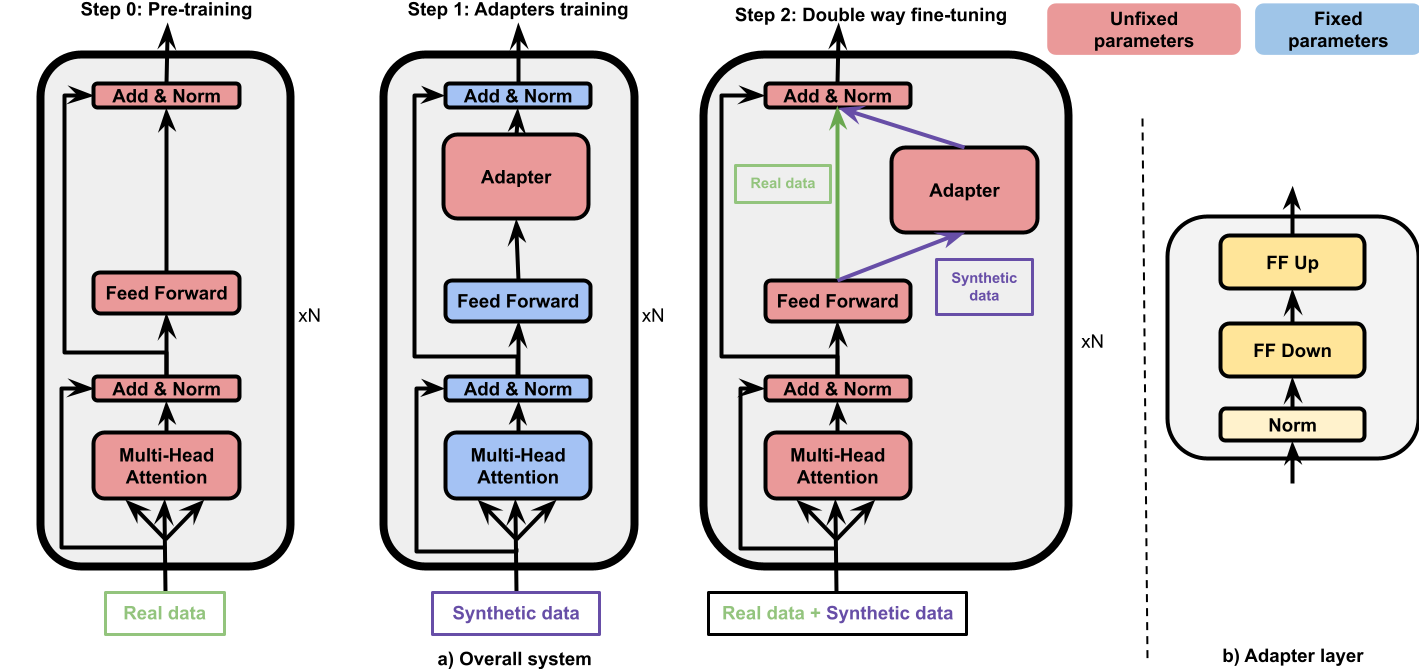
\includegraphics[width=\textwidth]{imgs/Overall_system.png}
    \caption{Overview of ``Double way Adapter fine-tuning"  within th context of an Conformer architecture}
    \label{fig:tts_conformer}
\end{figure}
Building upon the favorable results observed in previous chapters, which indicated that the Conformer model outperformed the regular Transformer for ASR tasks, the effectiveness of Adapters in Conformer and  considering that Synth++ \cite{hu2022synt++} was originally designed for the Conformer architecture, we decided to evaluate our DWAT within the Conformer architecture. Given that the TPA configuration of Adapters proved to be the most effective, we chose to implement it in our DWAT for the Conformer architecture. The DWAT with TPA is illustrated in Figure \ref{fig:tts_conformer}.

In this experiment, we employed the same pre-trained adult Conformer model used in previous chapters. This model comprises 12 layers of Conformer layers for the encoder, followed by 6 Transformer layers for the decoder, all with a hidden dimension of 512. The language model used is consistent with the experiments conducted with the Transformer model in the previous sections. Motivated by the insights gained from the exploration of hyperparameters in section \ref{sec:hyperparameter}, we opted for Adapters of size 512 in the Encoder only, using the TPA configuration. In term of training, Step 0 and step 1 were trained for 30 epochs while step 2 only used 10 epochs. 

\begin{table}[h]
    \centering
    \begin{tabular}{lr}
        \toprule
        Method & WER Score $\downarrow$ \\
        \midrule
        Adult model & 21.75\% \\
        \textit{Real} only & 12.28\% \\ \hline
        \textit{Unfiltered Synth$_2$} & 37.85\% \\
        \textit{Unfiltered Synth$_2$} + \textit{Real} & 12.30\% \\ 
        \textit{Synth$_2$} alone & 31.72\% \\
        \textit{Synth$_2$}+ \textit{Real} & 12.02\% \\ 
        Two step adaptation & 12.51\% \\ \hline
        Synth++ (norm double way) & 11.80\% \\
        DWAT & \textbf{11.64\%} \\
        \bottomrule
    \end{tabular}
    \caption{Scores for the different methods within the Conformer architecture}
    \label{tab:DWAT_conformer}
\end{table}

The results obtained from the extension of DWAT experiments using the Conformer architecture are presented in Table \ref{tab:DWAT_conformer}. The frozen adult model, referred as the Adult model, achieved a WER score of 21.75\%. When considering only real data (Real only), the WER score improved significantly to 12.28\%. Which is already outperforming the best results of the Transformer.

When using unfiltered synthetic data alone (\textit{Unfiltered Synth$_2$}) method, it resuted in a higher WER score of 37.85\%, showcasing, once again, the mismatch between synthetic and real data. However, when combined with real data (\textit{Unfiltered Synth$_2$} + \textit{Real}), the result are close to the real baseline with a WER score of 12.30\%. Similarly, using the filterd \textit{Synth$_2$} alone resulted in a WER score of 31.72\%, but when combined with real data (\textit{Synth$_2$} + \textit{Real}), the WER score decreased significantly to 12.02\%. This differ from the results observed in the Transformer architecture, as data filtering improved the WER score compared to the baseline.
Similarly to the Transformer, the two-step adaptation method yielded a WER score of 12.51\%. 

Further insights into the performance of the more sophisticated methods are provided in the context of the Conformer architecture. Specifically, the Synth++ method, which incorporates separated batch normalisation within each Convolution module for TTS data, achieved a WER score of 11.80\%. This contrasts with the results observed in the Transformer experiment, highlighting the efficiency of this approach specifically within Conformer models. In the other hand, the DWAT method consistently outperformed all other methods, showcasing a remarkable WER score of 11.64\%. These findings emphasise the effectiveness of both the Synth++ and DWAT methods in enhancing the Conformer architecture's performance on the given task.

It is important to highlight that while both Synth++ and DWAT demonstrate efficacy within the Conformer setup, the DWAT approach consistently outperforms other methods in both Transformer and Conformer configurations. This consistent superiority underscores the relevance and robustness of the DWAT approach in improving the overall performance of the models across different architectures.

In summary, the experimental results demonstrate the effectiveness of leveraging synthetic data, real data, and advanced adaptation methods within the Conformer architecture. The DWAT method, in particular, stands out as the most successful approach in minimising the WER.


\section{Summary and discussion}
\label{section:conclusions_tts}

In this chapter, we aimed to answer to the following research questions: \textit{Is it possible to use children's synthetic speech to extend the amount of children's data? How can we control the quality and speakers’ variability?}

% Summary 
We provide positive responses to both research questions through the introduction our a novel methodology: the Double way Adapter Transfer procedure, which combine Adapters and synthetic data augmentation for children's speech recognition. Our two-phase training strategy consist of the initial training of Adapter modules using synthetic data, followed by the fine-tuning of Adapters and the entire model weights using a hybrid dataset comprising both synthetic and real data. This distinctive dual-pathway approach resulted in notable improvement over baseline and previous techniques across various configurations. Importantly, our approach demonstrated robustness across different ASR architectures, TTS model fine-tuning parameters, Adapter sizes, number of epochs, and varying amounts of synthetic data. Furthermore, our study showcases the controllability of TTS output quality without necessitating direct modifications of the TTS model. This filtering process, performed before applying the DWAT, is achieved through the use of pre-trained x-vectors speaker embeddings and cosine similarity metrics between reference and generated utterances. This approach, improved from previous work which only used i-vectors \cite{wang2021towards}, allows the use of synthetic data which align more closely with desired characteristics of real children's speech, contributing to a more controlled augmentation process.

% Discussion
The promising performances observed with the DWAT pave the way for future research avenues. One potential avenue involves adopting an iterative methodology, dynamically incorporating newly generated TTS data while adjusting the proportion of real data. This iterative fine-tuning approach could potentially provide further insights into the interaction between synthetic and real data, offering opportunities to refine and optimise the training process for improved children's ASR models.
Another avenue for exploration could extend the DWAT framework to domains beyond the synthetic and real speech data. Investigating the adaptability and effectiveness of DWAT in diverse domains. In the context of children's ASR, the adult and children's speech domain could be an interesting first step towards this direction.
Furthermore, considering the rapidly evolving landscape of PETL approaches, the exploration of new modules as replacements for Adapters represents an new research direction. To this end, in the upcoming chapter, we delve into a comprehensive evaluation of various PETL alternatives, aiming to identify novel strategies for enhancing children's ASR systems.
% If Printing on DOUBLE SIDED pages, the second page should be white.
% Otherwise, comment the following command:
%\cleardoublepage{}
%
% -----------------------------------------------------------------------------
% BIBLIOGRAPHY
% Add the Bibliography to the PDF table of contents (not the document table of contents)
\pdfbookmark[0]{Bibliography}{bib}
\addcontentsline{toc}{chapter}{Bibliography}
% The bibliography style sheet
% Chose your preferences on the format of the entries and the Labels:
% IEEEtran: Used in general (recommended for IST Thesis)
%           Entries are labelled and sorted by appearance in the document
%           Labels are Numeric inside square brackets
\bibliographystyle{IEEEtran}
%
% Apalike:  Entries formatted alphabetically, last name first, with identation
%           Labels with Autor's Name and Year inside square brackets
%\bibliographystyle{apalike}
%
% Alpha:    Entries formatted with Autor's Name and Year, hanging identation
%           Labels with Autor's abbr. Names and Year inside square brackets
%\bibliographystyle{alpha}
%
% Acm:     Entries formatted with Autor's Name (small Caps), hanging identation
%          Labels are Numeric inside square brackets
%\bibliographystyle{acm}
% The following command resets the 'emphasis' style for bibliography entries
\normalem{}
% Name of your BiBTeX file
\bibliography{./Thesis-MSc-Bibliography} % Put here your own filename
%
% The following command modifies the 'emphasis' style for bibliography entries
\ULforem{}
% If Printing on DOUBLE SIDED pages, the second page should be white.
% Otherwise, comment the following command:
\cleardoublepage{}
%
% -----------------------------------------------------------------------------
% HERE GO THE APPENDIXES IF REQUIRED
% If not required just comment the blocks
%\appendix
%% First Appendix
%\pdfbookmark[1]{Appendix A}{appendix}
%% #############################################################################
% This is Appendix A
% !TEX root = ../main.tex
% #############################################################################
\chapter{Pathological speech detection through pre-trained models}
\label{chapter:appendixA}

%\section{Introduction}
In the domain of speech therapy, and specifically paediatric speech therapy, advancements in \acp{SLT} hold significant promise by providing automated tools for assessing pronunciation quality and identifying pathological conditions. While the primary focus of this thesis was to improve \ac{ASR} for children, we also contributed to the identification of pathological conditions from speech for adult speakers. This annexe provides an overview of these contributions.


\section{Pathological speech detection using x-vector embeddings}
\subsection{Introduction}
Speech has been proposed as a valuable biomarker for detecting various diseases, including neurological conditions, mood disorders, and respiratory diseases \cite{hauptman2019identifying,botelho2019speech}. However, challenges such as temporal and financial constraints, lack of medical community awareness, ethical concerns, and patient privacy laws impede the acquisition of medical data, posing significant obstacles to the development of health-related speech-based classifiers, especially for deep learning models.

Most existing classifiers rely on \ac{KB} features, often limited in capturing subtle symptoms and variations in disease severity. To address this limitation, some studies focus on speaker representation models, such as Gaussian Supervectors and i-vectors. For instance, Hauptman \textit{et al.} \cite{hauptman2019identifying} proposed i-vectors for \ac{PD} classification, while Laaridh \textit{et al.} \cite{laaridh17_interspeech} applied the i-vector paradigm to predict dysarthric speech evaluation metrics. The motivation behind using these speaker representations lies in their ability to model speaker variability, which should also include disease symptoms \cite{hauptman2019identifying}.

X-vectors are discriminative \ac{DNN}-based speaker embeddings, surpassing i-vectors in tasks like speaker and language recognition \cite{snyder2018x}. Despite initial doubts about the usability of such discriminative representations for disease detection as they have been trained on general datasets without diseased patients, recent studies have demonstrated their effectiveness. Indeed, x-vectors have been successfully applied to paralinguistic tasks such as emotion recognition \cite{pappagari2020x}, obstructive sleep apnea detection \cite{perero2019modeling}, and as a complement feature for Alzheimer’s disease detection \cite{zargarbashi2019multi}. In our work \cite{botelho2020pathological}, we investigated the hypothesis that speaker characteristics embedded in x-vectors, obtained from a single network trained for speaker identification using general data, contain sufficient information for the detection of multiple diseases. Furthermore, we aimed to assess whether this information persists even in the presence of language mismatch training, a phenomenon previously observed in speaker recognition \cite{snyder2017deep}. Specifically, we employ the x-vector model as a feature extractor to train \ac{SVM} for detecting two speech-affecting diseases: \ac{PD} and  \ac{OSA}.

\subsection{Speaker embeddings: i-vector and x-vector}
Speaker embeddings serve as fixed-length representations of variable-length speech signals, capturing essential information about the speaker. Traditional methods, such as Gaussian Supervectors \cite{kenny2007joint} derived from \ac{MAP}-adapted \ac{GMM-UBM} \cite{reynolds2000speaker} and i-vectors \cite{dehak2010front}, have been fundamental in speaker recognition.

I-vectors, until recently considered as state-of-the-art, extend the \ac{GMM} Supervector approach by modelling total variability as a low-rank space through factor analysis. Hauptman \textit{et al.} observed that i-vectors, while capturing total variability and speaker variability, also encompass information about speech disorders \cite{hauptman2019identifying}. For classification, they used reference i-vectors for healthy and \ac{PD} populations.

In contrast, x-vectors, proposed as an alternative to i-vectors, aim to discriminate between speakers by modelling specific characteristics. Unlike i-vectors, x-vectors exhibit robustness to data variability and domain mismatches, requiring shorter temporal segments for optimal performance. Typically, the x-vector system comprises three main blocks: \ac{TDNN} layers operating at the frame level, a statistical pooling layer for temporal aggregation (employing an attentive mechanism for importance weighting), and fully connected (Dense) layers for x-vector extraction.

\subsection{Experimental setup}
In our experiments, we used four corpora to determine the presence or absence of \ac{PD} and \ac{OSA}. Using specifically one of the European Portuguese corpus to train the i-vector and x-vector extractors. For each disease-related dataset, we compared three sets of features: \ac{KB} features, i-vectors, and x-vectors. All disease classifications were conducted using a \ac{SVM} classifier using leave-one-speaker-out cross-validation as an alternative to partitioning the corpora into train, development and test sets. Further details on the corpora, data representations, and classification method are provided below in Section \ref{sec:corpora_xvector_path}.

Additionally, our classification processes operate at the segment level, assigning speakers a final classification through a weighted majority voting mechanism. With this approach, predictions obtained for each segment uttered by the speaker are weighted based on the corresponding number of speech frames they contain.

\subsubsection{Corpora}
\label{sec:corpora_xvector_path}
In this section, we provide a description of the four datasets employed in our study. All utterances were segmented into 4-second-long segments using overlapping windows with a 2-second shift. Further details about each of these datasets can be found in Table \ref{tab:xvect_data}.

\begin{itemize}
  \item \textbf{Speaker Recognition:} Portuguese (PT-EASR) Corpus is a subset of the EASR (Elderly Automatic Speech Recognition) corpus \cite{hamalainen2014easr}. It comprises recordings of European Portuguese read sentences and was used for training both i-vector and x-vector models for a speaker recognition task. The dataset encompasses speakers aged from 24 to 91, with 91\% falling within the 60-80 age range. This specific age distribution was chosen with the intention of generating reliable speaker embeddings for this age group, particularly relevant to the diseases addressed in our study. The corpus was partitioned into training, development, and test sets in a ratio of 0.70:0.15:0.15, respectively.

  \item \textbf{\ac{PD} Detection:} The Portuguese \ac{PD} (PPD) Corpus, a subset of the FraLusoPark corpus \cite{pinto2016dysarthria} was employed. This corpus includes speech recordings of both French and European Portuguese healthy volunteers and \ac{PD} patients. For our experiments, we selected utterances of European Portuguese speakers reading prosodic sentences only.

  \item \textbf{Spanish \ac{PD} Detection}: We use the Spanish \ac{PD} (SPD) Corpus corresponds to a subset of the New Spanish Parkinson’s Disease Corpus, collected at the Universidad de Antioquia, Colombia \cite{orozco2014new}. For this experiment, we only used the read sentences subset. This corpus serves the purpose of investigating whether x-vector representations trained in one language (European Portuguese) can generalise effectively to another language, namely Spanish.
  
  \item \textbf{ \ac{OSA} Detection:} The corpus used in this experiment, is an extended version of the Portuguese Sleep Disorders (PSD) corpus \cite{botelho2019speech}. This corpus includes three tasks in European Portuguese: reading a phonetically rich text, reading sentences recorded during a cognitive load assessment task and spontaneous descriptions of an image. 
\end{itemize}


\begin{table}[h]
  \centering
  \begin{tabular}{cccccc}
  \hline
  Language & Task & Group & Speakers & Segments & Duration (h) \\
    \hline
  \multirow{5}{*}{PT} & Spk. Rcg. & - & 919 & 290,690 & 171.81  \\ \cline{2-6}
  & \multirow{2}{*}{PD} & Patient & 75 & 1,838 & 1.24 \\
  & & Control & 65 & 1,527 & 1.07 \\ \cline{2-6}
  & \multirow{2}{*}{OSA} & Patient & 30 & 1,793 & 1.10 \\
  &  & Control & 30 & 1,702 & 1.05 \\
  \hline
  \multirow{2}{*}{SP} & \multirow{2}{*}{PD} & Patient & 50 & 661 & 0.49 \\
  & & Control & 50 & 655 & 0.50 \\

  \hline
  \end{tabular}
  \caption{Detailed description of the different datasets used for pathology detection with speakers, segments and number hours information}
  \label{tab:xvect_data}
  \end{table}
  

\subsubsection{Knowledge based features}
For \ac{PD} classification, the \ac{KB} feature set was proposed by Pompili \textit{et al.} \cite{pompili2017automatic} and comprises 36 features from the eGeMAPS \cite{eyben2015geneva}, along with the mean and standard deviation of 12 \acp{MFCC} and log-energy. Additionally, the set includes the first and second derivatives of these coefficients, resulting in a 114-dimensional feature vector.

In the case of \ac{OSA} classification, the \ac{KB} feature set, as proposed in Botelho \textit{et al.} \cite{botelho2019speech}, includes the mean of 12 \acp{MFCC}, along with their first and second order derivatives, and 48 linear prediction cepstral coefficients. The set also covers the mean and standard deviation of the frequency and bandwidth of formant 1, 2, and 3, as well as the mean and standard deviation  of Harmonics-to-noise ratio, jitter, F0 at percentiles 20, 50, and 100, and mean and standard deviation  values for all frames and only voiced frames of Spectral Flux. All \ac{KB} features were extracted using openSMILE \cite{eyben2013recent}.

\subsubsection{Speaker embeddings}
\begin{table}[h]
  \centering
  \begin{tabular}{ccccc}
  \hline
  Layer & Contex & Total Contex & In $\times$ Out \\
  \hline
  TDNN1 & $[t-2, t+2]$ & 5 & $5F \times 256$ & \\
  TDNN2 & $\{t-2, t, t+2\}$ & 9 & $768 \times 256$ & \\
  TDNN3 & $\{t-3, t, t+3\}$ & 15 & $768 \times 256$ & \\
  TDNN4 & $\{t\}$ & 15 & $256 \times 256$ & \\
  TDNN5 & $\{t\}$ & 15 & $256 \times 512$ & \\
  stats pooling & $[0, T)$ & $T$ & $512T \times 1024$ & \\
  Dense 6 & $\{0\}$ & $T$ & $1024 \times 512$ & \\
  Dense 7 & $\{0\}$ & $T$ & $512 \times 512$ & \\
  softmax & $\{0\}$ & $T$ & $512 \times S$ & \\
  \hline
  \end{tabular}
  \caption{X-vector network architecture, used to train the x-vector embedding extractor with the PT-EASR dataset}
  \label{tab:xvect_description}
  \end{table}
  In the i-vector system, 19 \acp{MFCC} plus log-energy are given as input with non-speech frames removed using energy-based \ac{VAD}. Utterances are modelled with a 512-component full-covariance \ac{GMM}, resulting in 180-dimensional i-vectors. The entire process is implemented using Kaldi \cite{kaldi} over the PT-EASR corpus.

  For x-vectors, the network architecture is detailed in Table \ref{tab:xvect_description}, and x-vectors are extracted at the $6^{th}$ layer (Dense 6). Using 24-dimensional \ac{fbanks} as input features. The non-speech frames were removed using energy-based \ac{VAD}. This network was trained, using Pytorch \cite{paszke2019pytorch}on the PT-EASR corpus for speaker identification, using 100 epochs, cross-entropy loss, a learning rate of 0.001, a learning rate decay of 0.05 with a 30-epoch period, a batch size of 512, and a dropout value of 0.001.

\subsection{Results}
\begin{table}[h]
  \begin{tabular}{cc|ccc|ccc|ccc} \hline
                            &     & \multicolumn{3}{c|}{PD - Portuguese} & \multicolumn{3}{c|}{OSA}                      & \multicolumn{3}{c}{PD - Spanish} \\ \hline
  Features                  &     & Prec.        & Recall           & F1 Score        & Prec.     & Recall        & F1 Score      & Prec.       & Recall         & F1 Score       \\ \hline
  \multirow{2}{*}{KB}       & Seg & 64.5             & 64.6             & 64.5            & 64.8          & 64.9          & 64.8          & \textbf{79.0}   & \textbf{79.0}  & \textbf{79.0}  \\
                            & Spk & 72.2             & 72.3             & 72.1            & \textbf{82.0} & \textbf{81.7} & 81.6          & \textbf{87.1}   & \textbf{87.0}  & \textbf{87.0}  \\ \hline
  \multirow{2}{*}{i-vector} & Seg & 66.6             & 66.6             & 66.6            & 65.6          & 65.6          & 65.6          & 75.7            & 75.7           & 75.7           \\
                            & Spk & \textbf{75.6}    & \textbf{75.7}    & \textbf{75.6}   & 72.3          & 75.0          & 75.0          & 85.1            & 85.0           & 85.0           \\ \hline
  \multirow{2}{*}{x-vector} & Seg & \textbf{66.7}    & \textbf{66.8}    & \textbf{66.7}   & \textbf{73.3} & \textbf{73.3} & \textbf{73.3} & 77.2            & 77.2           & 77.1           \\
                            & Spk & 74.4             & 74.5             & 74.3            & 81.7          & \textbf{81.7} & \textbf{81.7} & 86.0            & 86.0           & 86.0 \\ \hline    
  \end{tabular}
  \caption{Precision, recall and F1 score results of the different pathologies detection with KB and speaker embeddings}
  \label{tab:xvect_results}
  \end{table}
The results of the different tasks are summarised in Table \ref{tab:xvect_results}. For \ac{PD} with Portuguese data, the findings indicate that speaker representations learned from out-of-domain data surpass the performance of \ac{KB} features. This supports our hypothesis that speaker embeddings not only capture information about the speaker but also model symptoms of the disease that \ac{KB} features may fail to include.

It is notable that x-vectors and i-vectors yield very similar results, with a slight advantage for x-vectors at the segment level and slightly better results for i-vectors at the speaker level. This observation suggests that while x-vectors offer stronger representations for short segments, i-vectors may perform better for longer segments. The application of a majority vote weighted by the duration of speech segments may favour the i-vector approach at the speaker level.

In the context of the \ac{OSA} task, x-vectors demonstrate superior performance compared to all other approaches at the segment level. Notably, they significantly showed around 8\% improvement over \ac{KB} features, providing further support for our hypothesis. However, it is essential to highlight that both x-vectors and i-vectors perform similarly at the speaker level. Interestingly, i-vectors, in this scenario, perform less effectively than \ac{KB} features. One possible explanation could be attributed to the fact that the PSD corpus incorporates tasks, such as spontaneous speech, which diverge from the read sentences included in the corpus used to train the i-vector and x-vector extractors. These tasks might be considered out-of-domain, which would explain why x-vectors outperform the i-vector approach.

The objective of the \ac{PD} Spanish experiment was to evaluate the efficacy of x-vectors trained in one language when applied to disease classification in a different language. Our findings reveal that \ac{KB} features outperform both speaker representations, possibly due to the language mismatch between the Spanish \ac{PD} corpus and the European Portuguese training corpus. However, it is noteworthy that, akin to the previous task, x-vectors demonstrate the ability to surpass i-vectors in an out-of-domain corpus.

To conclude, our experiments conducted on the European Portuguese datasets substantiate the hypothesis that speaker embeddings encompass pertinent information for disease detection. Notably, we identified evidence indicating that these embeddings capture information not represented by \ac{KB} features, validating the efficacy of our approach. Additionally, the observations suggest that x-vectors outperform i-vectors in tasks where the domain does not align with the training data, such as verbal task mismatch and cross-lingual experiments. This underscores the potential of x-vector embeddings as formidable alternatives to \ac{KB} feature sets for the detection of \ac{PD} and \ac{OSA}.


\section{The INESC-ID Multi-Modal System for the ADReSS 2020 Challenge}
\subsection{Introduction}
Later, we proposed to extend the aforementioned work by classifying \ac{AD} \cite{pompili2020inesc}. Indeed, existing studies have explored various approaches, including the use of syntactic or semantic features, plain acoustic methods, and combinations of speech and lexical parameters. However, the diversity in datasets and methodologies makes it challenging to compare these studies. To address this, the Alzheimer's Dementia Recognition through Spontaneous Speech (ADReSS) challenge was introduced, providing a common, statistically balanced, and acoustically enhanced dataset for researchers to test their approaches. In this work, we introduced a multi-modal system where both acoustic and textual feature embeddings were used for automatically distinguishing \ac{AD} patients
from healthy individuals. 

In the literature, studies focused on hand-crafted temporal and acoustic parameters from speech or linguistics or a fusion of both. For example, a study analysed temporal speech features \cite{konig2015automatic}. Another work employed over 350 features to capture lexical, syntactic, grammatical, and semantic phenomena from transcriptions of a picture description task \cite{fraser2016linguistic}. Finally, Gosztolya \textit{et al.} consider a set of feature including in conjunction demographic, acoustic, and linguistic features \cite{gosztolya2019identifying}.

More recently, a shift towards advanced architectures has been observed to overcome the limitations of traditional methods. For instance, Warnita \textit{et al.} \cite{warnita18_interspeech} used a gated \ac{CNN} on acoustic data, while Karlekar \textit{et al.} \cite{karlekar-etal-2018-detecting} explored linguistic impairments with \ac{CNN}, \acp{RNN}, and a combination. Finally, some work introduced a multi-modal feature embedding approach, based on n-gram, i-vector and x-vectors \cite{zargarbashi2019multi}.

Our work differs from previous studies in two aspects. First, by using contextual embedding vectors for text data, feeding into two systems: one employing Global Maximum pooling and bidirectional \ac{LSTM}-\acp{RNN} architectures, and the other based on statistical computation of sentence embeddings. Secondly, for audio, we use \ac{DNN} speaker embeddings extracted from pre-trained models. To the best of our knowledge, this is the first work which jointly uses automatically learned representations for both audio and textual data. Additionally, our approach is simpler and does not require training deep architectures.

\subsection{Corpus}
\begin{table}[h]
  \begin{center}
   \begin{tabular}{c|ccc}
    \hline
                    & \multicolumn{2}{c}{Train} & Test       \\ \cline{2-4}
                    & \textit{Control}     & \textit{AD}          & -          \\ \hline
  Audio Full        & 55min46s    & 1h14min     & 1h06min    \\
  Audio chunks      & 30min11s    & 26min31s    & 26min32s   \\
  \# Words (unique) & 6097 (567)  & 5494 (552)  & 5536 (602) \\ \hline
  \end{tabular}
  \caption{Statistical information on the ADReSS corpus}
  \label{tab:adress_data}
  \end{center}
  \end{table}
The ADReSS dataset comprises speech recordings and annotated transcriptions from 156 subjects, including 78 \ac{AD} patients and 78 healthy control speakers. The data is split into training (108 subjects) and test (48 subjects) sets. Participants provided descriptions of the Cookie Theft picture from the Boston Diagnostic Aphasia Examination \cite{goodglass2001bdae}. Speech recordings were segmentated using \ac{VAD} and normalised \cite{luz2020alzheimer}. The dataset contained both fully enhanced audio and normalised audio chunks. Our approach used both audio and transcriptions available. The transcriptions were annotated with disfluencies, filled pauses, repetitions and other complex events. The transcriptions contained 17,127 words, including 1,009 unique words. Additional details on the duration and size of the ADReSS dataset are provided in Table \ref{tab:adress_data}.
\subsection{Proposed system}
\begin{figure}[h]
  \begin{center}
  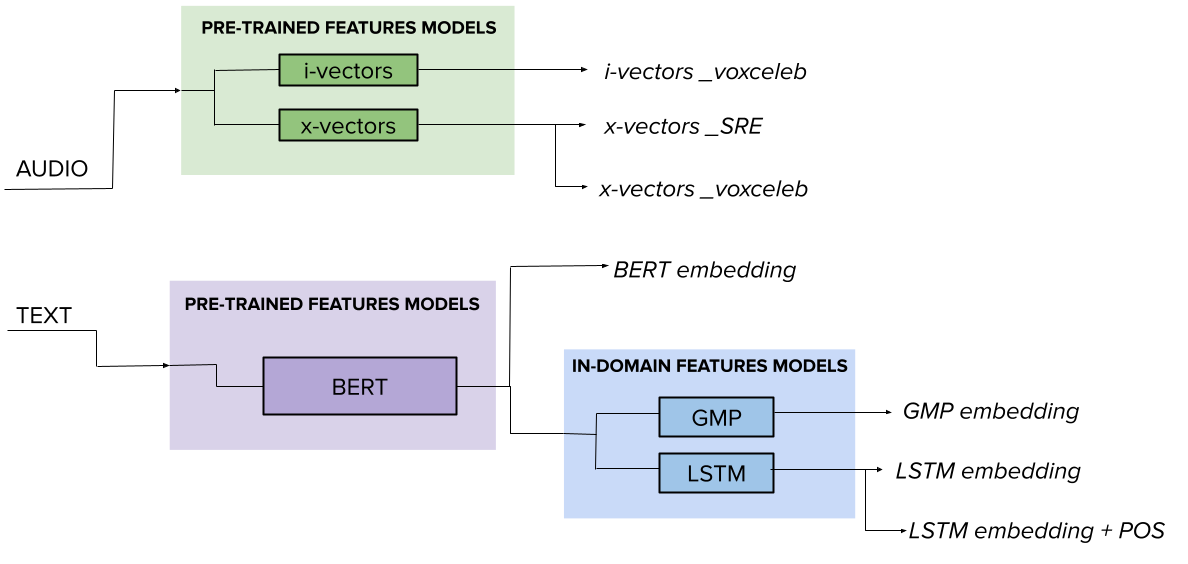
\includegraphics[scale=0.35]{imgs/ADReSS.png}  
  \caption{Overview of the multimodal system based on embedding approaches}
  \label{fig:adress_overview}
  \end{center}
\end{figure}
Our multi-modal framework, illustrated in Figure \ref{fig:adress_overview}, is based on the independent generation of acoustic and textual feature embeddings. Subsequently, we conduct an early fusion of the output of the two systems to create a single feature vector encapsulating a condensed representation of both speech and language characteristics of the utterance. The final classification is carried out using an \ac{SVM} classifier with a linear kernel. Further details of the two systems used in our experiments will be provided in the following sections.
\subsubsection{Acoustics modality}
The acoustic system incorporates i-vectors and x-vectors. Taking into consideration the small size of the ADReSS dataset, we preferred to use already existing pre-trained models to produce the acoustic feature embeddings, rather than training them using in-domain challenge data. For the x-vectors framework, both the SRE and Voxceleb models were employed. The SRE model was primarily trained on telephone and microphone speech using data from the Switchboard corpus, Mixer 6, and NIST SREs \cite{snyder2018x}. The Voxceleb model was trained on augmented VoxCeleb 1 and VoxCeleb 2 datasets, encompassing speech from speakers with diverse ethnicities, accents, professions, and ages \cite{snyder2018x,nagrani17_interspeech}. The VoxCeleb dataset was also used to build the i-vectors pre-trained model used in our experiments.

For all these pre-trained models, the inputs included 23 and 30-dimensional \acp{MFCC} extracted with the Kaldi toolkit \cite{kaldi} and non-speech frames were filtered out using \ac{VAD}. For x-vectors, 512-dimensional embeddings were extracted, while i-vectors, based on \ac{GMM-UBM}, were of dimension of size 400.

\subsubsection{Linguistic modality}
For the linguistic modality, we used two distinct methods to extract textual feature embeddings. Firstly, we explored training deep architectures on a relatively small corpus with dimensions of the same range as the one used in this challenge. Then, we compare this approach with a less data-intensive method based on extracting sentence embeddings using a pre-trained model. Both strategies use contextual word embeddings as input but produce different types of learned representations as output. In order to integrate information from linguistics in conjunction with the acoustic systems, the trained architectures were employed to extract linguistic features before the final classification layer. In this way, we obtain a single 768-dimensional feature vector for an entire description. The sentence embedding approach, on the other hand, provides a single 768-dimensional vector for each sentence of a description.

For both approaches, the initial pipeline step involved normalising the text data of the ADReSS dataset. Clean transcriptions were encoded into 768-dimensional context embedding vectors using a pre-trained English BERT model with 12 layers and 768 hidden units \cite{Bert}. Then, the first system is derived from the ComParE2020 Elderly Challenge baseline \cite{schuller2020interspeech}, involved training three neural models on top of contextual word embeddings: (i) a Global Maximum pooling, (ii) a bidirectional \ac{LSTM} (biLSTM) with an attention module, and (iii) the second model augmented with part-of-speech (POS) embeddings. The loss was evaluated during training on the development set.

The second system does not require an additional training phase, as representations are extracted from a pre-trained model to directly characterise linguistic deficits in \ac{AD}. Contextual word embeddings obtained for each word were used to compute fixed-size embedding vectors for each sentence by averaging the second to twelfth hidden layers of each word.

\subsection{Results}
\begin{table}[h]
  \begin{center}
  \begin{tabular}{lcccc}
  \hline
  & \multicolumn{1}{l}{\textbf{Accuracy}} & \multicolumn{1}{l}{\textbf{Precision}} & \multicolumn{1}{l}{\textbf{Recall}} & \multicolumn{1}{l}{\textbf{F1 Score}} \\
  \hline
  x-vectors\_Vox           & 0.6818                               & 0.6834                                & 0.6919                             & 0.6812                               \\
  x-vectors\_SRE              & \textbf{0.7273}                               & \textbf{0.7273}                                & \textbf{0.7273}                             & \textbf{0.7273}                               \\
  i-vectors\_Vox          & 0.6818                               & 0.7292                                & 0.6818                             & 0.6645                               \\
  i-vectors\_Vox\_x-vectors\_Vox & 0.7273                               & 0.7273                                & 0.7273                             & 0.7273                               \\
  i-vectors\_Vox\_x-vectors\_SRE      & 0.7273                               & 0.7351                                & 0.7273                             & 0.7250                                \\
  \hline
  \end{tabular}
  \caption{Results of different acoustic approaches on the development set}
  \label{tab:adress_acoustics}    
\end{center}
\end{table}

The results obtained using the different acoustic feature embeddings are summarised in Table \ref{tab:adress_acoustics}. Different independent models were explored, and an early fusion of the best acoustic results was performed. The x-vectors Voxceleb model generally achieved lower classification accuracy. However, when combining i-vectors and x-vectors both trained with VoxCeleb, the accuracy was comparable to x-vectors only trained on the SRE corpus, which represents the best acoustic result on the development set. These outcomes are slightly lower than those reported in similar works in the literature \cite{warnita18_interspeech,zargarbashi2019multi}. However, our approach is distinct from these previous studies as we use a smaller dataset and do not rely on \ac{DNN} training. To validate these results on the test set, we select the acoustic feature embeddings extracted from the pre-trained x-vectors SRE model for evaluation.
\begin{table}[h]
  \begin{tabular}{lcccc}
  \hline
& \multicolumn{1}{l}{\textbf{Accuracy}} & \multicolumn{1}{l}{\textbf{Precision}} & \multicolumn{1}{l}{\textbf{Recall}} & \multicolumn{1}{l}{\textbf{F1 Score}} \\ \hline
  Global Max Pool. & 0.7727                               & 0.7947                                & 0.7728                             & 0.7684                               \\
  LSTM-RNNs        & 0.8182                               & 0.8182                                & 0.8182                             & 0.8182                               \\
  LSTM-RNNs Pos    & 0.8636                               & 0.8667                                & 0.8637                             & 0.8634                               \\
  GMax/LSTM-RNNs/LSTM-RNNs-Pos                   & \textbf{0.9091}                               & \textbf{0.9091}                                & \textbf{0.9091}                             & \textbf{0.9091}  \\  
  %\textit{\textbf{Sentence emb.}  }                  & 0.6930                               & 0.6864                                & 0.6903                             & 0.6873  \\
  \textit{\textbf{Sentence emb. - maj. vote}}                    & 0.7727                               &0.7947                & 0.7728                           & 0.7684
  \\ \hline
  \end{tabular}
  \caption{Results of different linguistic approaches on the development set}
  \label{tab:res_dev_ling}
  \end{table}

  The results obtained with our various linguistic systems are shown in Table \ref{tab:res_dev_ling}, presenting the performance for features trained with three neural models, their fusion, and the sentence embedding approach. For the sentence embedding approach, the accuracy uses a majority voting strategy over the entire description. Our best classification result attained an accuracy of 90.91\% on the development set using the fusion of the linguistic feature sets generated by the three neural models. Comparing this result with the one obtained by sentence embeddings, we acknowledge that neural models outperform simpler strategies even with constrained training data. This was surprising and in contradiction with similar experiments performed with the acoustic system. We hypothesise that the large amount of contextual information provided by the BERT model is helpful in overcoming the limited size of the ADReSS dataset. Nevertheless, we suspect that the high accuracy attained with neural models may be too optimistic, due to the fact of having used the development set both for testing and evaluating the model’s loss. Thus, in spite of their lower outcome, the sentence embedding approach is selected as one of the systems to be evaluated on the test set. In fact, on the one hand, we think that they may represent a more reliable system, since do not require additional training. On the other hand, we also observe that they achieve higher classification scores when compared with a similar approach based on GloVe embeddings \cite{mirheidari2018detecting}, thus corroborating our decision.

  For a comprehensive evaluation of speech and language impairments in \ac{AD}, we performed an early fusion of the best results from both the acoustic and linguistic systems. This involved merging x-vectors with linguistic feature sets from three neural models. However, the results of the development set using this extended feature set did not yield additional improvements. Despite this, we selected the combined system as our primary choice for evaluation.

  \begin{table}[h]
    \begin{center}
    \begin{tabular}{llcccc}
    \hline
     & \textbf{Class} & \multicolumn{1}{l}{\textbf{Accuracy}} & \multicolumn{1}{l}{\textbf{Precision}} & \multicolumn{1}{l}{\textbf{Recall}} & \multicolumn{1}{l}{\textbf{F1 Score}} \\ 
                                         \hline
    Fusion of system   &  AD             & \multirow{2}{*}{\textbf{0.8125}}                     & 0.9412                                 & 0.6667                              & 0.7805                                \\
   & non-AD         &                                       & 0.7419                                 & 0.9583                              & 0.8364                                \\
    %                                     & Avg.           & \textbf{0.8125}                       & \textbf{0.8415}                        & \textbf{0.8125}                     & \textbf{0.8085}                       \\
    Sentence embedding &  AD             &  \multirow{2}{*}{\textbf{0.7292}}                                    & 0.8235                                 & 0.5833                              & 0.6829                                \\
     & non-AD         & \multicolumn{1}{l}{}                  & 0.6774                                 & 0.8750                              & 0.7636                                \\
    %                                     & Avg.           & 0.7292                                & 0.7505                                 & 0.7292                              & 0.7233                                \\
    x-vectors\_SRE     & AD             & \multirow{2}{*}{\textbf{0.5417}}                                      & 0.5417                                 & 0.5417                              & 0.5417                                \\
    & non-AD         & \multicolumn{1}{l}{}                  & 0.5417                                 & 0.5417                              & 0.5417                                \\ \hline
    %                                     & Avg.           & 0.5417                                & 0.5417                                 & 0.5417                              & 0.5417    \\ \hline
    \end{tabular}
    \caption{Results of different acoustic and linguistic approaches on the test set}
    \label{tab:adress_test}  
  \end{center}
    \end{table}


  For the evaluation, three systems were submitted: (i) a fusion of the best results from linguistic and acoustic systems, (ii) sentence embeddings, and (iii) the best acoustic system. Results on the test set, presented in Table \ref{tab:adress_test}, showed a consistent drop in performance compared to the development set, even for systems not requiring a training phase. The first system achieved the best result with an accuracy of 81.25\%, indicating the capability of deep architectures with contextual word embeddings to overcome dataset limitations. The acoustic system alone yielded the lowest accuracy at 54.17\%, suggesting room for improvement in adapting acoustic pre-trained models, for example, to better model elderly speech characteristics.



\section{Transfer Learning-Based Cough Representations for Automatic Detection of COVID-19}
\subsection{Introduction}
Finally, in our final work presented in this annexe \cite{SoleraUrea2021TransferLC}, we further extend the idea of using pre-trained representation to automatically detect COVID-19 from cough recordings. Indeed, the COVID-19 respiratory disease was declared a pandemic by the World Health Organisation in March 2020, with profound personal, societal, and economic consequences. Clinical diagnosis primarily relies on RT-PCR and antigen tests, but these methods have drawbacks such as significant costs, intrusive sample collections, and delays in diagnosis due to laboratory saturation. To address these challenges, there was a growing interest in developing reliable, cost-effective, immediate, and user-friendly tools to optimise screening campaigns for healthcare operators, institutions, and companies.

In our work, we contributed to the ComParE 2021 COVID-19 Cough Sub-challenge \cite{schuller21_interspeech}. Firstly, we employed transfer learning to develop COVID-19 classification subsystems using deep cough representation extractors, including \ac{TDNN-F} and \ac{CNN} embeddings, as well as \ac{PASE}+ features. Secondly, we integrate individual decisions from the three experts into a calibrated decision-level fusion system. This ensemble of expert subsystems, relying on cough representations, aims to generate well-calibrated log-likelihood scores across various operating points. The resulting output can be readily interpreted by human experts and seamlessly incorporated into the decision-making process.

Current research on the automatic detection of COVID-19 from speech or respiratory sounds builds on prior studies demonstrating the distinct effects of various respiratory diseases on these sounds. This approach has proven effective in detecting pertussis, asthma, pneumonia, and tuberculosis, among others \cite{pramono2016cough}. While conclusive evidence is still pending for COVID-19, preliminary findings suggest specific signatures of COVID-19 in coughs and speech that could potentially enable detection even in apparently asymptomatic individuals and differentiate it from other common respiratory diseases. Given the limited availability of labelled COVID-19 data, many approaches rely on transfer learning, data augmentation, and class balancing techniques.

The majority of previous work in this domain relies on \acp{CNN}. For instance, a pre-trained VGGish model \cite{Hershey2017} was employed as a generic audio feature extractor \cite{Chloe2020}. Other works fine-tune \acp{CNN} initially trained for cough detection for the purpose of COVID-19 detection \cite{Bagad2020,Imran2020}. Ensemble models incorporating both \acp{DNN} and \acp{CNN}, directly trained from scratch for COVID-19 detection, have also been proposed \cite{Chaudhari2021}. Additionally, certain studies  \cite{Han2021} leverage information about self-reported symptoms, encoding them as one-hot vectors and combining them either at the feature- or decision levels with traditional speech features.

\subsection{Corpora}
In this work, we used two datasets: the COVID-19 COUGH (C19C) corpus, provided in the ComParE 2021 COVID-19 Cough Sub-Challenge \cite{Chloe2020,Han2021} for evaluation, and the COUGHVID corpus \cite{Orlandic2020}, employed for training and fine-tuning transfer learning-based cough representation extractors. Silence segments were eliminated from both datasets using \ac{VAD}.

The COVID-19 COUGH (C19C) corpus is a subset of the Cambridge COVID-19 Sound database \cite{Chloe2020,Han2021}, consisting of 725 cough recordings from 397 participants with self-reported COVID-19 status labels (positive/negative). The corpus is distributed into a train (71 positives/215 negatives), development (48 positives/183 negatives), and a blind test set (208 samples) with gender-balanced subsets. 

In our preliminary analysis, it was observed that some files had a reduced bandwidth of 4 k\ac{Hz}, potentially corresponding to samples originally recorded at 8 k\ac{Hz}. Namely, 13, 8 and 8 narrow-band files were detected in the train, development and test subsets, respectively. This condition certainly reflects the reality of many real-world applications. However, we noticed that all the narrow-band recordings in the train and development subsets correspond to the COVID-19-positive class. To address this, a second version of the dataset, denoted as ``$\text{C19C}_{fullband}$", was created by removing narrow-band recordings from the original train and development subsets. This resulted in 273 samples in the training subset (58 positives/215 negatives) and 223 in the development subset (40 positives/183 negatives), while the test subset remained unchanged for consistent challenge evaluation conditions.

The COUGHVID corpus \cite{Orlandic2020} is a publicly open dataset consisting of non-curated recordings performed using lossy codification. In addition, the dataset includes a variety of conditions such as sampling rate, bandwidth, number of channels, and quality. Volunteers recorded their coughs and reported their COVID-19 status (positive/symptomatic/healthy), age, gender, and medical condition.
The dataset comprises 27,550 recordings, with 15,125 classified as coughs by an automatic cough detector. Of these, 10,763 have self-provided gender and COVID-19 status annotations, including 680 COVID-19 positives (395 male/285 female), 8,270 healthy (5,632 male/2,638 female), and 1,813 symptomatic (1,114 male/699 female). Additionally, a small fraction of the dataset was annotated by expert pulmonologists with information on various aspects, such as type of cough, presence of audible symptoms, diagnosis, and severity.

\subsection{Proposed system}

\subsubsection{TDNN-F embedddings}
X-vector embeddings are currently regarded as state-of-the-art speaker representations, surpassing other proposed representations like d-vectors and i-vectors. Motivated by the results of the two previous works mentioned earlier in this annexe, this study explores the applicability of x-vector-like embeddings to coughs, aiming to encode relevant information about the cough signal for medical insights.
The X-vector extractor is implemented using \ac{TDNN-F} architecture as proposed for in previous work of speaker recognition \cite{villalbaSRE182020}. Cough embeddings are 128-dimensional vectors obtained at the output of the final dense layer. The network undergoes two-stage training: initially, an age estimation and gender classification using a subset of the COUGHVID dataset was performed, and subsequently fine-tuning with expert-annotated data for tasks closely related to COVID-19 classification. These tasks include cough type, presence of dyspnea, presence of wheezing, diagnosis, and severity. The reason behind this fine-tuning step is the fact that these tasks are much closer to COVID-19 classification than age and gender. The given input features to the model consist of 30 \acp{MFCC} computed every 10 ms from 25 ms-length frames, following the \textit{egs/voxceleb/v2} Kaldi recipe \cite{kaldi}.

\subsubsection{CNN embedddings}
Reported \ac{CNN}-based approaches for COVID-19 detection suffer from some limitations such as the use of \acp{CNN} as generic audio feature extractors without task-specific tuning or relying on relatively small datasets for training. In contrast, our work addresses these limitations by leveraging transfer knowledge from the VGGish model, originally trained on a large corpus for audio classification, and subsequently fine-tuned for COVID-19 detection using the COUGHVID dataset.

The VGGish model \cite{Hershey2017}, is an adaptation of the VGG network \cite{Simonyan2015} for audio classification. It consists of four blocks of convolutional and pooling layers, followed by fully-connected layers and an output layer. In this work, a simplified version of the model is used and was pre-trained using 5.4 million hours of YouTube data. For our experiments, we used two different settings. In the first setting, the model serves as a pre-trained generic feature extractor with weights directly loaded from the original model. In the second setting, the model is fine-tuned for COVID-19 detection using a balanced subset of the COUGHVID dataset. The input to the VGGish network is log Mel-spectrogram features computed every 0.24 s from 0.96 s-length segments and the resulting embeddings are 256-dimensional vectors.

When fine-tuning, the last two layers, namely the dense and output layers, are replaced to facilitate training with limited data, with their weights initialised randomly. The entire \ac{CNN} is fine-tuned for 150 epochs using cross-entropy loss, the Adam optimiser with a learning rate of $10^{-5}$, and a batch size of 64. The fine-tuning is conducted on a balanced subset of the COUGHVID dataset, consisting of 680 positive and 680 negative cough recordings, with 80\% used for training and 20\% for development.

\subsubsection{PASE+ embedddings}
Our study incorporates the problem-agnostic speech encoder model, \ac{PASE}+ \cite{Pascual2019,Ravanelli2020}, where targets are learned directly from the
signal in an unsupervised manner. \ac{PASE}+ features are derived from a shared encoder with a SincNet-based layer \cite{Sincnet}, seven convolutional blocks, and a Quasi-\ac{RNN} layer. The encoder output is connected to twelve workers, each designed for specific tasks like reconstruction of the waveform, \ac{LPC}, \acp{MFCC}, prosody, \ac{fbanks}, gamma tone, and some binary discrimination tasks. Two \ac{PASE}+ extractors were used: one pre-trained on Librispeech \cite{librispeech} and another trained from scratch on COUGHVID data. Both are trained for 150 epochs, creating 256-dimensional feature vectors for each frame every 10 ms.

\subsubsection{COVID-19 condition classification}
The key aspect of our study is to employ transfer learning to address the limited COVID-19 data for training. For classification, three \acp{SVM} were used respectively on \ac{TDNN-F} embeddings, \ac{CNN} embeddings, and \ac{PASE}+ features. In practice, \ac{TDNN-F} embeddings are directly input to the \ac{SVM}. \ac{CNN}-based embeddings are derived from cough segments and subjected to majority voting for the final decision. \ac{PASE}+ features are averaged across the sequence and fed to the \ac{SVM} classifier. The \acp{SVM} are trained on both the C19C and $\text{C19C}_{fullband}$ datasets, exploring various kernels, data normalisations, and class balancing methods. Hyperparameters are optimised through grid-search on development subsets, and linear logistic regression is applied to combine system decisions with scaling factors. The regression approximates log-likelihood ratios, thus, a theoretically determined decision threshold can be used for making hard decisions.

\subsection{Results}
\begin{table}[h]
  \begin{center}
    
  \begin{tabular}{c|c|c|c}
  \hline
  \multicolumn{1}{c|}{\textbf{System}} & $dev$ & $dev_{fullband}$ & $test$ \\ \hline
  \multicolumn{4}{c}{\textbf{ComParE 2021 CCS Sub-challenge Baseline}} \\ \hline
  {\scriptsize OPEN}SMILE & 61.4 & 53.0 & 65.5 \\
  {\scriptsize OPEN}XBOW\textsubscript{2000} & 64.7 & 56.5 & 72.9 \\
  D{\scriptsize EEP}S{\scriptsize PECTRUM}+SVM & 63.3 & 57.3 & 64.1 \\
  {\scriptsize AU}DEEP\textsubscript{-60 dB} & 67.6 & 57.3 & 67.6 \\
  End2You & 61.8 & - & 64.7 \\
  Fusion of Best & - & - & 73.9 \\ \hline
  
  \multicolumn{4}{c}{\textbf{TDNN-F Embeddings}} \\ \hline
  Trained COUGHVID\textsubscript{Step1} & 68.8 & 63.6 & - \\
  Fine-tuned COUGHVID\textsubscript{Step2} & 68.1 & 62.3 & - \\ \hline
  
  \multicolumn{4}{c}{\textbf{CNN Embeddings}} \\ \hline
  Pre-trained YouTube & 66.9 & 62.4 & - \\
  Fine-tuned COUGHVID & 71.2\textsuperscript{+} & 65.6 & 62.3\textsuperscript{+} \\ \hline
  
  \multicolumn{4}{c}{\textbf{PASE+ Features}} \\ \hline
  Trained Librispeech & 63.1 & 61.7 & -  \\
  Trained COUGHVID & 67.4 & \textbf{66.8}\textsuperscript{+} & 64.1\textsuperscript{+} \\ \hline
  
  \multicolumn{4}{c}{\textbf{Calibrated Fusion}} \\ \hline
  Fusion of experts & \textbf{72.3}\textsuperscript{+} & 66.1 & 69.3\textsuperscript{+} \\ \hline
  \end{tabular}
  \caption{Performance results (unweighted average recall-UAR) on the COVID-19 COUGH (C19C) corpus}
  \label{tab:res_covid}

\end{center}
  \end{table}

  Table \ref{tab:res_covid} shows the comparison between ComParE 2021 CCS baselines and our proposed systems. All systems were separately trained on both the C19C and $\text{C19C}_{fullband}$ subsets, and evaluations were conducted on the corresponding dev and $\text{dev}_{fullband}$ subsets. The reported test results are based on the best individual systems trained on the C19C and $\text{C19C}_{fullband}$ datasets (marked with +), presented in terms of \ac{UAR}.

  Our proposed system demonstrates competitive performance compared to baseline systems. The \ac{TDNN-F} x-vector embeddings-based expert, trained initially on gender classification and age regression tasks using COUGHVID data, achieves a \ac{UAR} of 63.6\% on devfullband. However, fine-tuning using a multi-task setting does not significantly enhance the cough representations, suggesting potential overfitting for some subtasks with limited data.
  
  The \ac{CNN} embeddings pre-trained on YouTube videos exhibit reasonable performance, improving to 65.6\% \ac{UAR} after fine-tuning with COVID-19-specific data. The \ac{PASE}+ features, trained with COUGHVID data, yield the best performance among the three expert systems, with a development \ac{UAR} of 66.8\% and a test \ac{UAR} of 64.1\%. Notably, the \ac{PASE}+ extractor achieves a 5.1\% absolute improvement in\ac{UAR} when trained with COVID-19-specific data, indicating the significant benefit of such data.
  
  The fusion of the best x-vector (Trained COUGHVID$_{Step1}$), \ac{CNN} (Fine-tuned COUGHVID), and \ac{PASE}+ (Trained COUGHVID) experts yields a \ac{UAR} of 72.3\% on development (1.1\% absolute improvement from the best expert) and 69.3\% on test when trained on the C19C datasets. The underperformance on the $\text{C19C}_{fullband}$ subset warrants further analysis but may be attributed to the low number of COVID-19 positive examples.

%We leverage transfer learning to develop a set of COVID-19 classification subsystems based on deep cough representation extractors called experts. Individual decisions of three experts are fed to a calibrated decision-level fusion system. This ensemble of expert subsystems based on cough representations is expected to produce well-calibrated log-likelihood scores over a wide range of operating points. The output can be more easily interpreted by a human expert and incorporated into the decision-making process. Our results show competitive performance compared to hand-crafted features, although they are still far from those required to become a reliable tool to assist COVID-19 screening.

\section{Conclusion and future work}
In these three distinct research works done within the context of this thesis, we employed pre-trained embedding extractors as tools for detecting pathologies from speech or cough signals. These embeddings can be used in two different ways: functioning either directly as feature extractors or undergoing fine-tuning for specific tasks. Our findings present promising results, indicating that embeddings trained on substantial amounts of data may contain valuable health-related information.

We began by exploring the replacement of knowledge-based features with task-agnostic speaker representations in multiple disease detection. Focusing on x-vector embeddings trained with elderly speech data, our experiments with European Portuguese datasets supported the hypothesis that discriminative speaker embeddings, particularly x-vectors, contain relevant information for disease detection that knowledge-based features may fail to represent. Notably, x-vectors proved to be more suitable than i-vectors for tasks with domain mismatches, such as verbal task mismatches and cross-lingual experiments. Future endeavours include training the x-vector network with augmented and multilingual datasets and extending our approach to other diseases.

Moving to the context of \ac{AD} classification, we adopted a multi-modal approach, leveraging automatically learned feature representations. Our investigation covered both acoustic and linguistic, exploring feature embedding vectors from pre-trained models and training deep neural architectures. By combining these approaches, we achieved an accuracy of 90.91\% and 81.25\% on the development and test sets, respectively. Notably, acoustic systems demonstrated a greater need for data to improve predictive ability, especially in the presence of potential \ac{ASR} errors. Future work may involve analysing the impact of \ac{ASR} error transcriptions in the final classification and exploring robust acoustic methods tailored to \ac{AD} speech characteristics.

Lastly, our focus shifted to the ComParE 2021 COVID-19 Cough Sub-challenge. Leveraging transfer learning, we developed three expert classifiers: \ac{TDNN-F} embeddings, \ac{CNN} embeddings, and \ac{PASE}+ features. While our results demonstrated competitive performance compared to baseline systems, caution is warranted due to the limited data. To enhance the reliability of COVID-19 screening tools, larger datasets are recommended for better learning of cough representations, coupled with more suitable backend classifiers. Future exploration could include recurrent neural networks with attention mechanisms to capture temporal dynamics, \ac{SSL}, multi-task \ac{TDNN-F} network-based cough embeddings and assessing the suitability of \ac{PASE}+ features as an alternative input representation.

Collectively, these contributions showcase the diverse applications of advanced technologies in addressing challenges in health-related tasks using pre-trained representations, ranging from COVID-19 screening through cough analysis to \ac{AD} classification and beyond, ultimately paving the way for impactful advancements in \acp{SLT}. 
%% If Printing on DOUBLE SIDED pages, the second page should be white.
%% Otherwise, comment the following command:
%\cleardoublepage{}
%% Second Appendix
%\pdfbookmark[1]{Appendix B}{appendix}
%% #############################################################################
% This is Appendix B
% !TEX root = ../main.tex
% #############################################################################
\chapter{Sefl-supervised learning as feature extractor for children's ASR}
\label{chapter:appendixB}

\section{Introduction}
% Very short intro SSL
In light of the increasing availability of large amount of unlabeled speech data, there has been a need to efficiently extract general-purpose knowledge from it. Consequently, SSL has experience notable advances and has gained substantial attention in recent years especially in the context of low-resource tasks. SSL refers to a training paradigm where a model learns representations from unlabeled speech data without relying on explicit labels or annotations. This approach yields discernible enhancements in performance across various applications such as speech recognition, speaker identification, and emotion recognition \cite{baevski2020wav2vec}. Traditionally, SSL models can be used in two manners: firstly, as a feature extraction to replace human-designed features \cite{yang21c_interspeech,chang2021exploration}, and secondly, as a model initialisation accomplished by concatenating prediction layers and fine-tuning the entire model \cite{fan2022draft,jain2023wav2vec2,wang2021fine,li2021accent}.

% Children ASR SSL
In recent years, an incrase number of research focus on using SSL models for children ASR. One notable avenue observed in the literature involves the fine-tuning of SSL models exclusively using children's data [] or through a combination of adult and children's data []. These efforts have yielded improved performances, showcasing the adaptability of SSL models to the nuances inherent in the speech patterns of children. Conversely, an alternative strategy has emerged by using Adapters to adapt SSL models specifically to children's speech characteristics subsequently followed by the full model, Adapters included, fine-tuning \cite{fan2022draft}. This initial training, allow to reduce the complexity associated with the conventional process of fine-tuning the entire model directly with children speech.
%  Our motivation
The observed successes of SSL as an initialisation for fine-tuning in the context of children's ASR underscore its efficacy as a new training paradigm. However, the exploration of SSL models as front-end feature extractors, compared to the conventional hand-crafted features, despite its use and success for adult speech \cite{yang21c_interspeech,chang2021exploration} remains unexplored for childen's ASR. Motivated by these considerations, this chapter undertakes a comprehensive review of various SSL models, evaluating their potential as novel feature extractors in the domain of children's ASR.
\section{Self-supervised pre-trained models}

\begin{table}[htbp]
    \centering
    \begin{tabular}{ccccccc}
      \toprule
      Method & Architecture & \#Params & Stride & Input & Corpus & \\%Pretraining \\ 
      \midrule
      FBANK & - & 0 & 10ms & waveform & - & \\%- \\
      APC [7] & 3-GRU & 4.11M & 10ms & FBANK & LS 360 hr \\%& 360 hr F-G \\
      VQ-APC [32] & 3-GRU & 4.63M & 10ms & FBANK & LS 360 hr \\%& 360 hr F-G + VQ \\
      NPC [33] & 4-Conv, 4-Masked Conv & 19.38M & 10ms & FBANK & LS 360 hr \\%& 360 hr M-G + VQ \\
      Mockingjay [8] & 12-Trans & 85.12M & 10ms & FBANK & LS 360 hr \\%& 360 hr time M-G \\
      TERA [9] & 3-Trans & 21.33M & 10ms & FBANK & LS 960 hr\\%& 960 hr time/freq M-G \\
      wav2vec 2.0 Base [14] & 7-Conv, 12-Trans & 95.04M & 20ms & waveform & LS 960 hr\\%& 960 hr M-C + VQ \\
      wav2vec 2.0 Large [14] & 7-Conv, 24-Trans & 317.38M & 20ms & waveform & LL 60k hr\\%& 60k hr M-C + VQ \\
      HuBERT Base [35] & 7-Conv, 12-Trans & 94.68M & 20ms & waveform 960 hr& LS 960 hr \\%& 960 hr M-P + VQ \\
      HuBERT Large [35] & 7-Conv, 24-Trans & 316.61M & 20ms & waveform & LL 60k hr\\%& 60k hr M-P + VQ \\
      \bottomrule
    \end{tabular}
    \caption{Overview of different SSL architectures used in this chapter}
    \label{tab:SSL_models}

  \end{table}


Traditionally, SSL models can be categorised into two distinct approaches: generative modeling and discriminative modeling. In this section, we will focus on summarising a selection of SSL models, presented in Table \ref{tab:SSL_models}, with a particular emphasis on their differences.

\subsection{Generative modeling}
% List a couple of model and explain their differences
Generative modeling has emerged as a prevalent approach for learning speech representations for SSL. Generally, generative models are trained to generate speech frames based on their learned speech representations with or without the help of context. For instance, the Autoregressive Predictive Coding (APC) model adopts a language model-like training paradigm, where a Recurrent Neural Network (RNN) generates future frames predicted from the past frames. Building upon this foundation, the Vector-Quantized APC (VQ-APC) model enhances the generative process by incorporating vector-quantization layers for more compact representations.
The Mockingjay model takes inspiration from BERT-like pretraining techniques by masking input acoustic features along the time axis and subsequently regenerating the masked frames. Expanding upon this concept, the Temporal Encoder Representations from Acoustics (TERA) model introduces an additional layer of complexity by masking bins in the frequency axis alongside the temporal axis. Finally, the Non-autoregressive Predictive Coding (NPC) model combines elements from both APC and Mockingjay by substituting the RNN in APC with a CNN layers and modifying the future frames generation process into a masked reconstruction.

\subsection{Discriminative modeling}
\begin{figure}[ht]
    \centering
    \subfigure[Illustration of the Wav2vec2 architecture taken from \cite{baevski2020wav2vec}]{\label{fig:wav2vec2}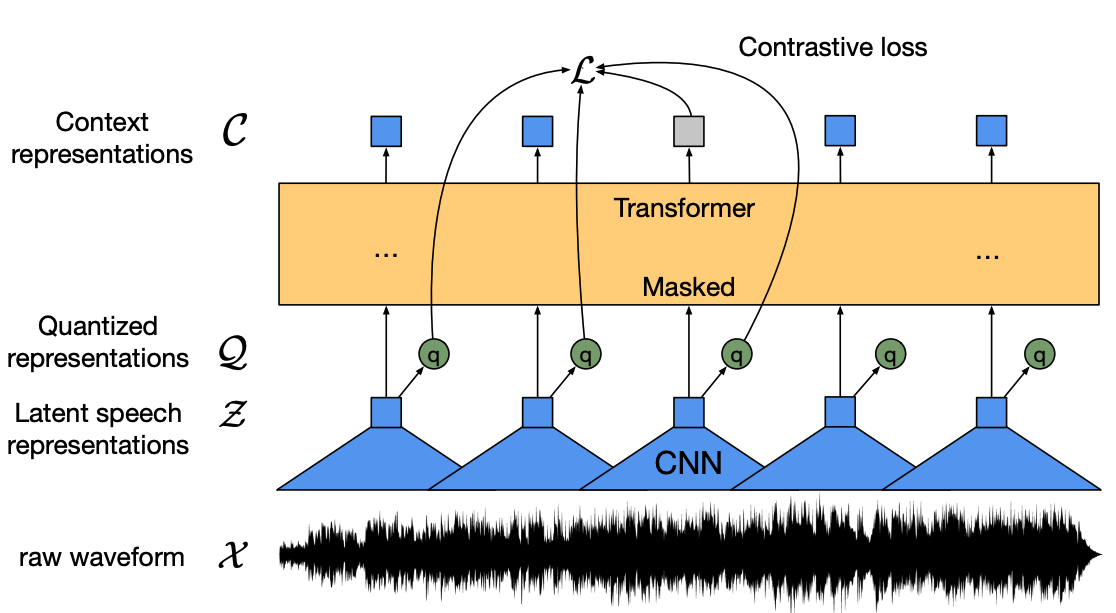
\includegraphics[width=0.48\textwidth]{imgs/wav2vec2.png}}
    \subfigure[Illustration of the HuBert architecture taken from \cite{hsu2021hubert}]{\label{fig:Hubert}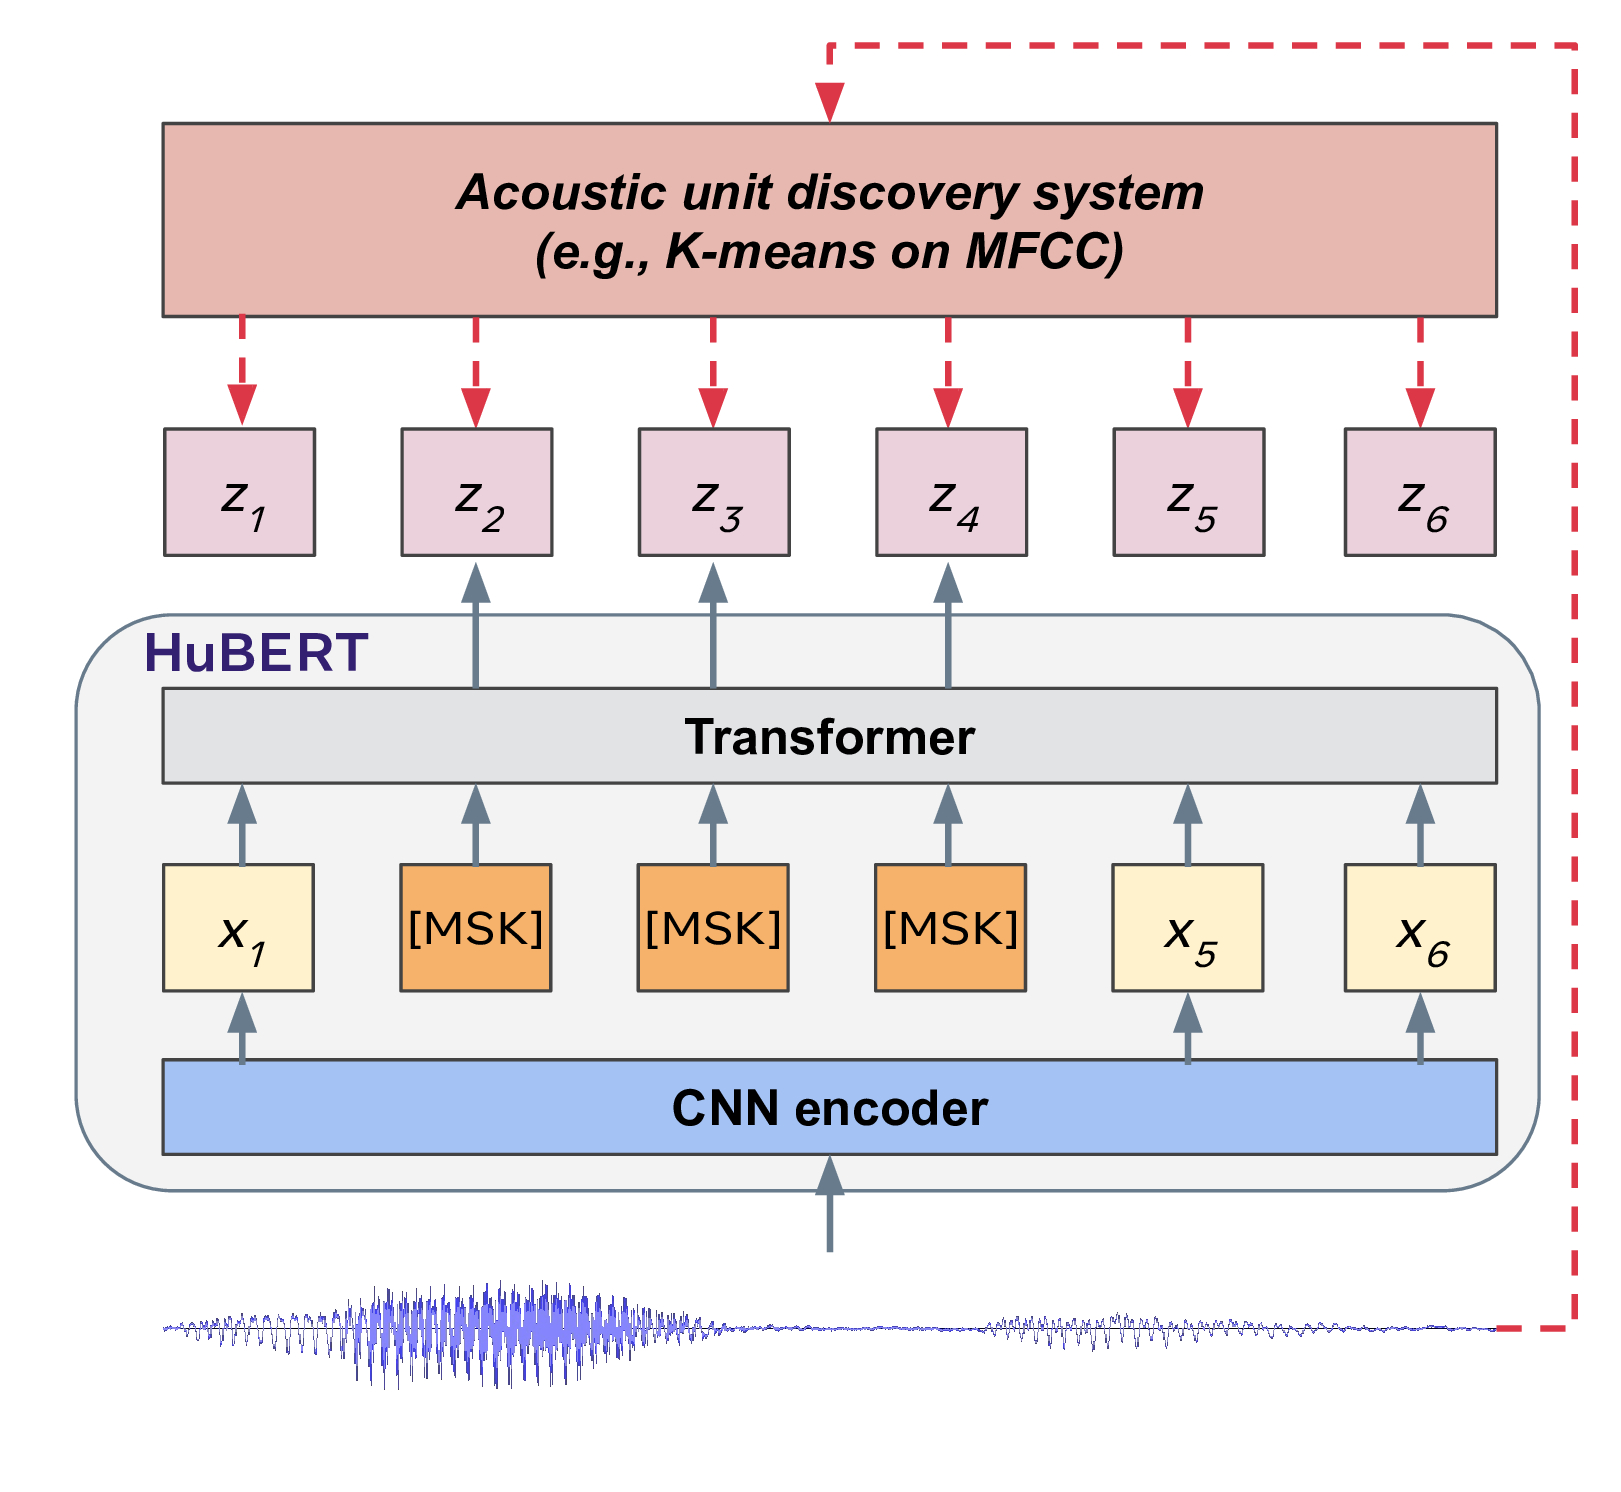
\includegraphics[width=0.48\textwidth]{imgs/Hubert.png}}
    \caption{Overview of the discriminative SSL Wav2vec2 and HuBert models}
\end{figure}
% Explain Wav2Vec2 and Hubert    
The success of discriminative modeling has been notably pronounced with the introduction of the contrastive loss, a technique where the model discerns between correlated positive samples and negative samples. The underlying intuition is that positive samples should exhibit closer representations in comparison to their negative counterparts. A prominent exemplar of this approach is evident in the Wav2Vec2 model, which has demonstrated promising potential in learning speech representations. The Wav2Vec2 model achieves this by masking latent representations of the raw waveform and formulating a contrastive task over quantized speech representations. A more detailed representation of Wav2Vec2 architecture is displayed in figure \ref{fig:wav2vec2}. Later, moving away from the contrastive loss, the work of [] proposed the HuBert model. This model introduces a novel methodology by incorporating BERT's token prediction via offline clustering on representations. Specifically, the HuBert model use a BERT-like training that consumes masked continuous speech features to predict pre-determined cluster assignments. The labels assigned to the masked locations during clustering serve as the predicted targets. Importantly, the predictive loss is selectively applied solely over the masked regions, compelling the model to learn robust high-level representations of unmasked inputs in order to accurately infer the targets of the masked ones. The HuBert architecture is shown in figure \ref{fig:Hubert}.
\section{Experimental setup}
In our experimental setup, we used the Self-Supervised Speech Pre-training and Representation Learning (s3prl) toolkit\footnote{https://github.com/s3prl/s3prl}. The s3prl allow the modular use of pre-trained SSL models, called upstream, to perform various downstream tasks. In order to evaluate the efficiency of different SSL models as features extractor for children's ASR, we froze the pre-trained models's weight to extract embedding representation of the speech signal as new acoustic features. All the differents SSL upstream models used in our experiments are listed along with detailed informations regarding their architectures in table \ref{tab:SSL_models}. Notably, each of these models underwent self-supervised pre-training on either 360 or 960 hours of LibriSpeech \cite{librispeech} (denoted as LS 360hr and LS 960hr, respectively) or on an extensive 60 thousand hours of LibriLight data \cite{librilight} (referred to as LL 60k hr) . 
The ASR downstream task was conducted using a 2-layered Bidirectional Long Short-Term Memory (BiLSTM) architecture with 1024 units, optimised with a CTC loss. The training spanned 800 thousand iterations, with a learning rate set at $1.0\dot 10^{-4}$. Additionally, a dropout rate of $0.2$ was applied to the BiLSTM architecture to increase robustness. Limited by the large size of some SSL model, we decided to used a subset of the Myst \cite{MyST} dataset, using 77 hours of speech for training, by removing the longest utterances in the train and validation sets. A detailed description of the filtered Myst data is provided in table \ref{tab:ssl_myst}.
\begin{table}[h!]
    \caption{My Science Tutor Children Speech Subset Corpus statistics}
    
    \begin{center}
    \begin{tabular}{r|c|c|c}
    \hline
     & Training & Validation     & Test   \\ \hline
    \# of utterances & 23594   & 3959    & 4079  \\ 
    \# of speakers & 559  & 79    & 91  \\ 
    \# of hours & 77   & 12    & 13  \\ \hline
    \end{tabular}
    \label{tab:ssl_myst}
    \end{center}
    \end{table}

% Phoneme based experiments
Additionally, we evaluated the  

\section{Results}

%For these models, the training process is separated into two stages. The first phase of training is self-supervised, which implies that no labels are used during training. The objective of this first phase is to present a large amount of unlabelled data to the system so that it learns a good speech representation. The second stage of learning is supervised fine-tuning, in which the model is taught to predict specific phonemes using the robust representation acquired in the previous stage with the help of a small amount of labelled data.
%In this category, two models stand out as state-of-the-art: Wav2Vec 2.0 \cite{baevski2020wav2vec} and HuBert \cite{hsu2021hubert}. As a preliminary experiment, to asses the usability of such frameworks for children ASR, we trained a BiLSTM model using the output of a variety of frozen self-supervised systems. For this experiment we used a subset of 50h of the Myst corpus \cite{MyST}, and the preliminary findings are displayed in the table \ref{tab:ssl}
\begin{table}[ht]
\centering
\begin{tabular}{lcc} 
\hline
SSL upsteam & UER $\downarrow$ & WER $\downarrow$ \\ 
\hline
Fbanks & 12.29\% & 35.14\% \\ 
\hline
TERA \cite{tera} & 11.31\% & 31.80\% \\
Audio Albert \cite{chi2021audio} & 12.28\% & 34.69\% \\
Wav2Vec2.0 Base & 7.37\% & 19.76\% \\
Wav2Vec2.0 Large & 7.00\% & 18.76\% \\
Distill HuBERT \cite{chang2022distilhubert} & 9.22\% & 25.75\% \\
HuBERT Base & 7.40\% & 19.77\% \\
HuBERT Large & \textbf{6.03\%} & \textbf{15.41\%} \\
\hline
\end{tabular}
\caption{Results without language model of different Self-supervised models as feature extractors}
\label{tab:ssl}
\end{table}
Table \ref{tab:ssl} present the results of the comparaison between various SSL pre-trained model as feature extractors for children's ASR. We provide Unit error rate (UER) as well as WER. Fbanks are established as a baseline, yielding a UER of 12.29\% and a WER of 35.14\%. In terms of generative SSL models, TERA \cite{tera} and Audio Albert \cite{chi2021audio} surpass Fbanks, exhibiting improvements in both UER ,11.31\% and 12.28\% respectively and WER with 31.80\% and 34.69\% respectively. Turning to discriminative SSL, the Wav2Vec2.0 Base and Wav2Vec2.0 Large demonstrate substantial enhancements in performance, achieving UER values of 7.37\% and 7.00\%, and WER of 19.76\% and 18.76\%, respectively. The distilled version of HuBERT \cite{chang2022distilhubert} outperforms Fbanks but falls behind the Wav2Vec2.0 models in terms of both UER and WER with 9.22\% UER and 25.75\% WER. Finally, HuBERT Base and HuBERT Large emerge as the top-performing SSL models, boasting the lowest UER with respectively 7.40\% and 6.03\% and WER of 19.77\% and 15.41\%. We observed that the best performing models are the large discriminative pre-trained on a large amount of speech data.

The results suggest that large Discriminative models, particularly HuBert Large, demonstrate superior performance compared to other SSL models and Fbanks as featuress extractor for children ASR. Notably, even though no language model where used in this experiment, the results are of the same order as those reported in previous the different chapters of the thesis obtained with a transformer and a transformer language model. Showing the benefic of using frozen pre-trained SSL models as feature extractor for children ASR.

\section{Analysis of the extracted features}
\begin{figure}
  \begin{center}
  \centering
  \subfigure[]{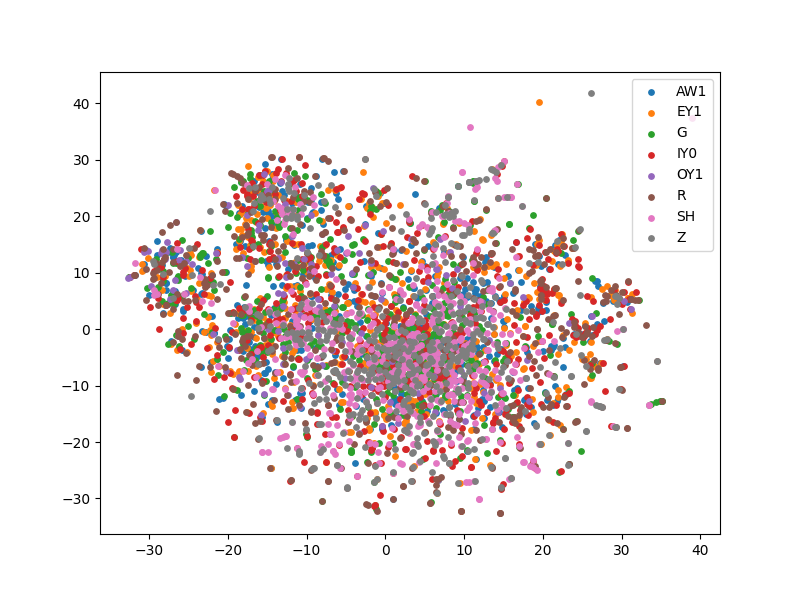
\includegraphics[width=0.49\textwidth]{imgs/fbank_umap_plot.png}} 
  \subfigure[]{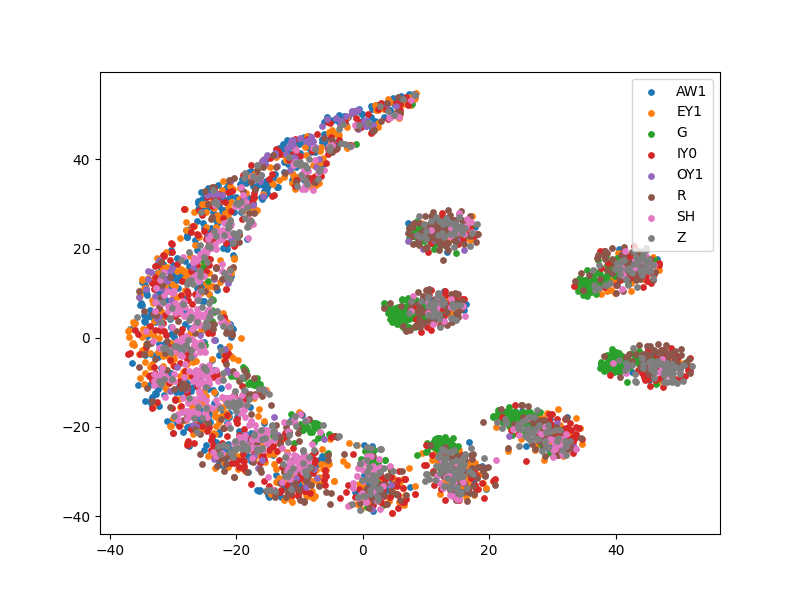
\includegraphics[width=0.49\textwidth]{imgs/tera_umap_plot.png}} 
  \subfigure[]{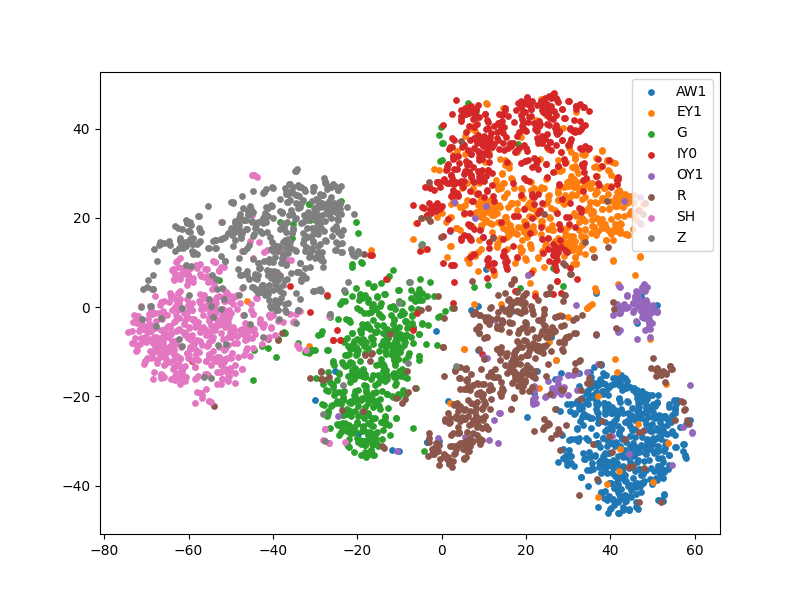
\includegraphics[width=0.49\textwidth]{imgs/wav2vec_umap_plot.png}}
  \subfigure[]{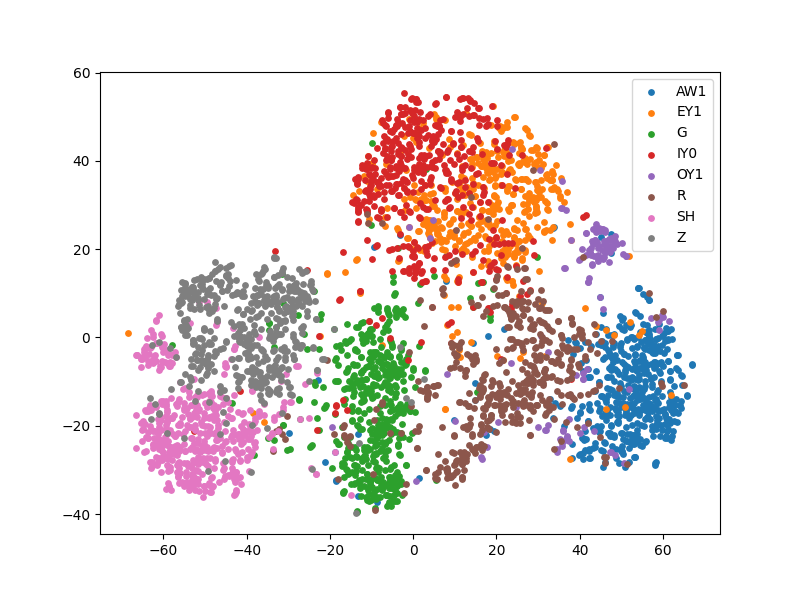
\includegraphics[width=0.49\textwidth]{imgs/hubert_umap_plot.png}}
  \caption{(a) Fbanks (b) TERA (c) Wav2Vec 2.0 (d) HuBERT \\ T-SNE plot of the different extracted features using the same speech data using phoneme labels}
  \label{fig:tsne_ssl}  
\end{center}
\end{figure}
% Explain experiment
In this section, we delve in more detail into the distinct features extracted from various models, aiming to better understand the notable performance differences observed between Wav2Vec 2.0 and HuBERT, in contrast to generative models like TERA and traditional filterbanks. In a first step we aligned our children's speech data to obtain phoneme alignments using the Montreal Forced Aligner \cite{mcauliffe2017montreal}. %These phoneme alignments serve as the foundation for extracting different features corresponding to each phoneme.

% Explain the plot procedure
Therefore, for each phonemes present in a utterance we obtained a variable-length feature sequences corresponding the extracted features for the different frames where the phoneme has been aligned. In order to get a single vector for each phoneme, we average these sequences. It is noteworthy that silence frames have been excluded. This operation is repeated for a subset of one thousand utterances of children speech in order to gather different exemple of the same phoneme from different speaker and different context. Subsequently, t-SNE (t-Distributed Stochastic Neighbor Embedding) plots are generated for each of the studied models. 

% Plot interpretation
The t-SNE plots are depicted in Figure \ref{fig:tsne_ssl}. We observe that traditional filterbanks features form a cloud points witn no structure. This lack of structure suggests that the fbanks features do not inherently exhibit phoneme-related information.
Moving on to the t-SNE plot for TERA features, clusters are observable, but these clusters do not align with phoneme. This observation indicates that while TERA features capture information from speech, they not encode phoneme-specific information, as evidenced by the presence of mixed phonemes within the different clusters.
In contrast, both Wav2Vec 2.0 and HuBERT exhibit highly similar plots, wherein distinct clusters corresponding to different phonemes are evident. This finding suggests that the features extracted from Wav2Vec 2.0 and HuBERT inherently capture phonemic information, even though no explicit phoneme annotations were provided during training. The presence of these phoneme-related clusters indicates that the usage of these features facilitate the ASR task by implicitly encoding phoneme information.



\section{Conclusions and future work}
% Conclusion 

% Careful about the language used and future work
However, it is crucial to emphasise that the outcomes and findings of our experiments are highly dependent on the language used. Specifically, all the SSL models were pre-trained using English language, which align with the language of the children dataset used in this experiment. Consequently, the generalisability of our results may be limited when applied to different languages. Using a different language could potentially result in decreased performances, as the SSL models may not be as adept at capturing the linguistic nuances and acoustic characteristics specific of that particular language \cite{phdthesis}. To address the language-dependent nature of our results, future work could explore the efficacy of employing multi-lingual SSL models, such as XLS-R \cite{babu2021xlsr}.
%Where Base, and Large represent the same model with different number of parameters (in the order Base $<$ Large).
%Even though we did not use a language model in this pilot experiment, the results are of the same order as those reported in section \ref{section:exp} obtained with a transformer and a transformer language model. Such results demonstrate that SSL learns substantial speech characteristics. For future research, we aim to explore in depth what information is encoded in SSL models and why they work well on children, and how we may use this knowledge to enhance children's ASR.

%% If Printing on DOUBLE SIDED pages, the second page should be white.
%% Otherwise, comment the following command:
%\cleardoublepage{}

% -----------------------------------------------------------------------------
% And this is THE END of the IST Thesis Document
\end{document}